%
\documentclass[11pt]{thesis} % draft

\title{Algorithmic Meta-Creativity}
\author{Fania Raczinski}
\date{March 2015}

\begin{document}

\pagestyle{empty}
\todototoc
\setcounter{tocdepth}{1}  % needed to display the todos
\listoftodos[List of Todos]
\clearpage

% !TEX root = ../main.tex

\begin{titlepage}
\begin{center}

Institute of Creative Technologies\\
De Montfort University

\vspace{2cm}

\textsc{\huge \href{http://fania.uk}{Fania Raczinski}}

\vspace{2cm}

% 
\includegraphics{dmu}\\[2cm]

\textsc{\Huge \bfseries Web Collider}

\vspace{1.5cm}

{\huge \bfseries A pataphysical methodology for applying creativity to exploratory search}

\vspace{2cm}

\emph{Supervisors:}\\
{Prof. Hongji \textsc{Yang}}\\
{Prof. Andrew \textsc{Hugill}}\\
{Dr. Sophy \textsc{Smith}}\\
{Prof. Jim \textsc{Hendler}}

\vspace{1.5cm}

\large \textit{A thesis submitted in partial fulfilment of the requirements\\ for the degree of Doctor of Philosophy}

\vfill

Created: {25th March 2015} --- Last Saved: {\today}\\
% Wordcount: \wordcount

\end{center}
\end{titlepage}


% FRONT
\pagestyle{plain}
\frontmatter

\phantomsection
\addcontentsline{toc}{part}{PREFACE}
\partimage[width=\textwidth]{spiral_pre.pdf}
\part{\texorpdfstring{PRE\smiley{}}{PREFACE}}
% !TEX root = ../main.tex

\pagestyle{empty}

\chapter{TL;DR}
\label{abstract}

{\Large \textbf{Algorithmic Meta-Creativity}}
Fania Raczinski

\vspace{0.5cm}
ABSTRACT\footnote{``Too long; didn't read''}

A pataphysical methodology for applying creativity to exploratory search

\vspace{1cm}

{\Large \textbf{Creativity, Pataphysics and Computers}}

Absurd Obscure French Pseudo Philosophy

Creative Computing

Art

Practice-Based Research

Exploratory Search

pata.physics.wtf

Interpretation/Evaluation

% ANDREW JOHNSTON
% This thesis is concerned with the design of interactive virtual musical instruments intended to augment acoustic instruments in live performance. For the purposes of this work, a virtual musical instrument is defined as a computer system designed to facilitate musical expression and/or exploration. The aim of the research is to develop understanding of the nature of virtual instruments and how musicians interact with them. The approach has been to use participatory design techniques to develop a series of virtual instruments for use in live performance and then to examine closely the experiences of musicians who use them.
% An interaction design strategy which uses simulated physical models to medi- ate between the sounds produced by acoustic instruments and computer generated sounds and visuals has been developed. In this approach, a simple physical sys- tem is modelled in software and characteristics of acoustic sounds are mapped to forces and other parameters which affect the model. In response the model moves in ways that are physically realistic. These movements are then used as parameters to control video and audio synthesis.
% Using a research approach which draws on action research, design science and participatory design, a series of virtual instruments which use this interaction tech- nique were developed and used in live performances. A set of initial design criteria which guided development were identified. In order to refine these criteria and better understand the impact that using these virtual instruments has on musicians’ music- making, a series of user studies were conducted. A number of expert musicians used the virtual instruments and discussed their experiences. These sessions were video-recorded, transcribed and analysed using grounded theory techniques.
% The results of the study identified three modes of interaction with the virtual in- struments: instrumental, conversational and ornamental. Musicians interacting with the virtual instruments in instrumental mode emphasise the importance of being in control and being able to trust that the instrument will respond consistently. When musicians use a virtual instrument ornamentally, they surrender detailed control of the generated sound and visuals to the computer, allowing it to create audio-visual layers that are added to the musicians’ sound. The more complex, (and difficult to design for) conversational interaction involves the sharing of control between the mu- sician and the virtual instrument. The balance of power is in flux, allowing the virtual instrument to talk back to the musician, reflecting and transforming the sonic input in ways that move the performance in new musical directions.
% The contributions of this thesis are therefore:-
% • a set of virtual musical instruments which use a unique interaction paradigm in which simulated physical models mediate between live sounds produced on acoustic instruments and computer generated sounds and visuals;
% • a theory of musician-virtual instrument interaction; and
% • a set of design criteria informed by practice and user studies.



\clearpage

% !TEX root = ../main.tex

\pagestyle{empty}

\chapter{Dedication}

For Dave.

\begin{CJK}{UTF8}{min}
  物の哀れ
\end{CJK}



% \begin{verbatim}
%       _____           _____
%    ,ad8PPPP88b,     ,d88PPPP8ba,
%   d8P"      "Y8b, ,d8P"      "Y8b
%  dP'           "8a8"           `Yd
%  8(              "              )8
%  I8                             8I
%   Yb,                         ,dP
%    "8a,                     ,a8"
%     "8a,                 ,a8"
%       "Yba             adP"
%        `Y8a         a8P'
%         `88,     ,88'
%           "8b   d8"
%            "8b d8"
%             `888'
%               "
% \end{verbatim}

\clearpage

% % !TEX root = ../main.tex

\pagestyle{empty}

\chapter{Declaration}



\clearpage

% % !TEX root = ../main.tex

\pagestyle{empty}

\chapter{Acknowledgements}


\begin{itemize}
\item Hongji Yang
\item Andrew Hugill
\item Sophy Smith
\item Jim Hendler
\item Dave
\item Mum
\item God\ldots
\end{itemize}

\clearpage

% % !TEX root = ../main.tex

\pagestyle{empty}

\chapter{Publications}
\label{pubs}

James Sawle, \textbf{Fania Raczinski} and Hongji Yang (2011) \emph{"A Framework for Creativity in Search Results"}. The 3rd International Conference on Creative Content Technologies, CONTENT'11. Rome, Italy. Pages 54-57.

Andrew Hugill, Hongji Yang, \textbf{Fania Raczinski} and James Sawle (2013) \emph{"The pataphysics of creativity: developing a tool for creative search"}. Routledge: Digital Creativity, Volume 24, Issue 3. Pages 237-251.

\textbf{Fania Raczinski}, Hongji Yang and Andrew Hugill (2013) \emph{"Creative Search Using Pataphysics"}. Proceedings of the 9th ACM Conference on Creativity and Cognition, CC'13. Sydney, Australia. Pages 274-280.

\grule

De Montfort University has granted me a 3 year bursary of £13.500 per year covering living costs and tuition fees.

A £1000 travel fund has been awarded by the DMU Faculty of Technology for travel to Australia, Sydney for the Creativity and Cognition conference in July 2013.

\grule

De Montfort University Institute of Creative Technologies PhD showcase at the Phoenix Cube Gallery, Leicester, 15-18 August 2014.

De Montfort University Leicester Media School Launch Showcase, 05 November 2014.

\clearpage

% % !TEX root = ../main.tex

\pagestyle{empty}

\chapter{About}
\label{about}

Fania Raczinski

European Baccalaureate from the European School Karlsruhe, Germany\\
BSc Computer Science (Europe) from the University of Leicester\\
MSc Creative Technologies from De Montfort University

\clearpage


\begin{SingleSpace}
% \phantomsection
% \addcontentsline{toc}{chapter}{Short Contents}
% \setcounter{tocdepth}{0}% chapters and above
% \shorttoc{Short Contents}{0}
% \clearpage
\phantomsection
% \renewcommand*{\contentsname}{Long Contents}
\setcounter{tocdepth}{1} % sections and above
\tableofcontents
\clearpage
\end{SingleSpace}

\phantomsection
% \addcontentsline{toc}{chapter}{List of Figures}
\listoffigures
\clearpage

\phantomsection
% \addcontentsline{toc}{chapter}{List of Tables}
\listoftables
\clearpage

% \phantomsection
% \addcontentsline{toc}{chapter}{List of Equations}
% \listofmyequations{}
% \clearpage

\phantomsection{}
\addcontentsline{toc}{chapter}{List of Code Snippets}
\listoflistings{}
\clearpage

\phantomsection
\addcontentsline{toc}{chapter}{List of Acronyms}
\printnoidxglossary[type=acronym]
\clearpage


% MAIN
% \pagestyle{fancy}
\pagestyle{plain}
\mainmatter

\phantomsection
\addcontentsline{toc}{part}{HELLO WORLD}
\partimage[width=\textwidth]{spiral_hello.pdf}
% \part{\texorpdfstring{H$\Sigma$LL$\Theta$ W$\Theta$RLD}{HELLO WORLD}}
\part{\texorpdfstring{\textipa{HELLO WORLD}}{HELLO WORLD}}
% !TEX root = ../main.tex

\chapter{Introduction}
\label{ch:introduction}

\startcontents[chapters]

\vfill

\begin{alltt}\sffamily
Feeling a movement of pity,
discovered the induction coil,
cette irraisonnee induction,
and entered the opening in the wall.

Only by some recherche movement,
apres coup et sous forme d'introduction,
opening his seized manuscript,
the enemy made within the enclosure of the vineyard.

Which he had thrown off at the beginning of his labor,
in opening so exactly at the,
than the thirst of my paternity.

We can then start at once,
and whose informing voice had consigned me to the hangman,
as any person at all conversant with authorship may satisfy himself at.
\end{alltt}

\newpage
% {\Large\sffamily\scshape\textbf{1.0 \quad Introduction Contents}}
% \vspace{0.5cm}
\minicontents
\spirals

This thesis describes \acf{AMC}. In other words it is about using creative computing to achieve computer creativity.

The project is transdisciplinary;\marginpar{§~\ref{ch:methodology}} it is heavily inspired by the absurd French pseudo-philosophy pataphysics\marginpar{§~\ref{ch:pataphysics}} and draws from a wide range of subject areas such as computer science, psychology, linguistics, literature, art and poetry, languages and mathematics.

The research\marginpar{§~\ref{ch:foundations}} included exploring what it means to be creative as a human, how this translates to machines, how pataphysics relates to creativity and how creativity should be evaluated in machines\marginpar{§~\ref{ch:interpretation}}.

Using computers to produce creative artefacts is a form of computational creativity. Using creative techniques computationally is creative computing. \ac{AMC} spans the two---whether this is to achieve a creative or non-creative output. It is the use of digital tools (which may not be creative themselves) and the way they are used forms the creative process or product. 

Creativity in humans needs to be interpreted differently to machines\marginpar{§~\ref{s:theoryanalysis}}. Humans and machines differ in many ways, we have different `brains/memory', `thinking processes/software' and `bodies/hardware'. Too often creative output by machines is judged as we would a human's. 

Computers which are truly artificially intelligent might be capable of true artificial creativity. Until then they are (philosophical) zombie robots: machines that behave like humans but aren't conscious. The only alternative is to see any computer creativity as a direct or indirect expression of human creativity using digital means and evaluate it as such. \ac{AMC} is neither machine creativity nor human creativity---it is both. By acknowledging the undeniable link between computer creativity and its human influence (the machine is just a tool for the human) we enter a new realm of thought. How is \ac{AMC} defined and evaluated? This thesis addresses this issue. 

\begin{enumerate}
  \item a practical demonstration of \ac{AMC}
  \item a theoretical framework to help interpret and evaluate products of \ac{AMC}
\end{enumerate}

The outcome of step (1)\marginpar{§~\ref{ch:implementation}} is presented as a website---\url{pata.physics.wtf}---written in \num{5} different programming languages\footnote{Python, \acs{HTML}, \acs{CSS}, Jinja, JavaScript}, making calls to \num{6} external web services\footnote{Microsoft Translate, WordNet, Bing, Getty, Flickr and YouTube}, in a total of over \num{3000} lines of code\footnote{\num{2864} lines of code, \num{489} lines of comments - as of 08 Dec 2015} spread over \num{30} files.

The main purpose of the system above is to demonstrate the three creative \emph{patalgorithms} in the context of exploratory \acf{IR}\marginpar{§~\ref{s:algorithms}}. A browsing rather than a search engine, it presents results in various formats such as sonnets and golden spirals. The system partially automates the creative process, generating results on demand, which allows users to focus on their own personal artistic evaluation rather than production.

Immediate inspirations\marginpar{§~\ref{ch:inspirations}} come from fictional character \textit{Doctor Faustroll} created by French absurdist and `father' of pataphysics Alfred Jarry \autocite*{Jarry1996}, the fantastic taxonomy of the \textit{Celestial Emporium of Benevolent Knowledge} by magical realist Jorge Luis Borges \autocite*{Borges2000} and \textit{A Hundred Thousand Billion Poems} by pataphysician and Oulipo co-founder Raymond Queneau \autocite*{Queneau1961}, amongst others.

To address step (2) above, I explored the problem of objective evaluation and interpretation\marginpar{§~\ref{ch:interpretation}} of subjective creativity specifically in regards to \ac{AMC}. I have argued that the most appropriate way to approach this is by looking at five objective constraints (person, process, product, place, purpose) and seven subjective criteria (novelty, value, quality, purpose, spatial, temporal, ephemeral) holistically and by understanding that humour and art `lie in the ear and eye of the beholder'.

This resulted in an \emph{interpretation framework}\marginpar{§~\ref{s:framework}} visualised as an evaluation matrix (\num{5} constraints x \num{7} criteria)\marginpar{\faicon{object-group}~\ref{fig:matrix}} which can be used to qualitatively and/or quantitatively measure the creativity of a given \ac{AMC} artefact:

\begin{enumerate}
  \item a set of scales that can be used to approximate a `rating' for the creative value of an artefact,\marginpar{§~\ref{s:sec}}
  \item a set of criteria to be considered using the scales above,\marginpar{§~\ref{s:oec}}
  \item a combined framework for evaluation.\marginpar{§~\ref{s:framework}}
\end{enumerate}


\section{Motivation}

Computers\marginpar{§~\ref{ch:technology}} are binary machines; the world is black and white to them (0 and 1, on and off). Programmers can run abstract high-level commands which are executed in sequence (with fast speeds giving the illusion of multitasking). They are precise, structured, logical, and generally abide by strict standards. Computers can only be creative if they are given clear instructions as to how. \acl{IR} is generally focused on relevance of results in regards to the query.

\begin{quotation}
  The Analytical Engine has no pretensions whatever to \emph{originate} anything. It can do \emph{whatever we know how to order it} to perform. \sourceatright{\autocite[Ada Lovelace, in][her emphasis]{Menabrea1842}}
\end{quotation}

Pataphysics\marginpar{§~\ref{ch:pataphysics}} emerged during the \textit{Belle Époque}\footnote{1871---1914} in France and has either directly or indirectly influenced various artistic movements such as Dada, Symbolism, Surrealism, Oulipo and Absurdist Theatre. Pataphysics is highly subjective and particular, values exceptions, the imaginary and the mutually incompatible.

Creativity\marginpar{§~\ref{ch:creativity}} is often studied at various levels (neurological, cognitive, and holistic/systemic), from different perspectives (subjective and objective) and characteristics (combinational, exploratory and transformative). It is usually defined in terms of value, originality and skill.

Combining computing with pataphysics seems impossible---although the antinomies below (juxtaposing principles in computing on the left with ideas from pataphysics on the right) highlight just how intriguing a possible combination of the two would be.

\begin{itemize}
  \item Polymorphism (generalisation) opposes particularity.
  \item Precision opposes exceptions and contradictions.
  \item Logic and structure oppose the imaginary and paradox.
  \item Cross-compatibility opposes the mutually exclusive.
  \item Responsiveness opposes the specific.
  \item Relevance opposes the creative.
\end{itemize}

This apparent dichotomy of computing and pataphysics is alluring. Christian B{\"o}k argued that pataphysics ``sets the parameters for the contemporary relationship between science and poetry'' \autocite*{Bok2002}. Pataphysics suddenly seems like the perfect choice infusing computers (science) with creativity (poetry).

Combining pataphysics with creativity\marginpar{\faicon{table}~\ref{tab:creatpata}} is easier. The ideas of combinatorial, exploratory and transformative creativity map quite nicely onto some pataphysical concepts such as clinamen, syzygy, antinomy and anomaly. 

Another motivating factor for this project was the lack of research in the particular area of creative computing\marginpar{§~\ref{ch:creativity}} in general. The discipline of computational creativity has emerged fairly recently\footnote{The first International Conferences on Computational Creativity ran in 2010 for example.} from a background in \ac{AI}. It appears to focus a lot more on the outcome of a product that would be judged creative rather than the actual process. Creative computing focuses on producing creative algorithms which may or may not have creative outputs. This was first addressed in \autocite{Raczinski2013}\marginpar{§~\ref{s:dc243article}} and later expanded into a definite description of this new discipline \autocite{Hugill2013c}.

\spirals

My personal interest in this project comes from a background in computer science and a longstanding interest in art. Most recently I managed to successfully combine my technical skills with my creative side for a Master of Science degree in Creative Technologies at \ac{DMU}\footnote{A passive interactive installation, augmenting a live video stream of users with interactive elements using motion tracking algorithms. See \url{msc.fania.eu} \autocite{Raczinski2010}.}. 


\section{Questions}

Research dealing with subjective ideas and concepts like creativity throws up a lot of questions. My intention is to address them all throughout this thesis, although some of them will not have definite binary answers. An attempt to answer them can be found in the conclusion chapter~\ref{s:answers}\marginpar{§~\ref{s:answers}}.

\begin{itemize}
  \item What is the relationship between pataphysics and creativity?
  \item How is computer creativity related to \ac{AI}?
  \item Should we distinguish between computationally automated or emulated creative processes and the programmer's input?
  \item How can a machine's creative output be evaluated?
  \item How can \ac{IR} be infused with creativity?
\end{itemize}


\section{Methodology}
\label{s:intromethod}

This project combines research\marginpar{§~\ref{ch:methodology}} in science and art making it transdisciplinary.

\begin{description}[leftmargin=3cm]
  \item [Pataphysics] Literature, Philosophy, Art, Poetry
  \item [Creativity] Cognitive Science, \ac{AI}, \ac{DH}
  \item [Technology] \ac{IR}, \ac{NLP}, Web Development
\end{description}

\begin{description}[leftmargin=3cm]
  \item [Epistemology] Transdisciplinary, subjective
  \item [Methodology] Creative computing, exploratory, experimental
  \item [Methods] Artefact, literature synthesis, algorithm design, theoretical framework, critical reflection and analysis, rapid incremental prototyping
\end{description}

The general process of my project was as follows.

\begin{enumerate}
  \item Critically analyse and synthesise existing literature,\marginpar{\textspiral~\ref{p:lit}}
  \item develop pataphysical algorithms,\marginpar{\textspiral~\ref{p:practice}}
  \item design a system to demonstrate algorithms,\marginpar{\textspiral~\ref{p:practice}}
  \item develop a website as an artefact,\marginpar{\textspiral~\ref{p:practice}}
  \item define an evaluation and interpretation framework,\marginpar{\textspiral~\ref{p:theory}}
  \item analyse results.\marginpar{\textspiral~\ref{p:analysis}}
\end{enumerate}


\section{Contributions}

The key contributions to knowledge described in this thesis are:

\begin{itemize}
  \item Three pataphysical search algorithms (clinamen, syzygy and antinomy).
  \item A creative exploratory search tool demonstrating the algorithms \url{pata.physics.wtf}.
  \item A set of 7 subjective criteria and 5 objective constraints for defining creativity.
  \item A combined framework for evaluating and interpreting creativity.
\end{itemize}


\section{Publications}

Some chapters (especially \nameref{ch:foundations} and \nameref{ch:interpretation})\marginpar{§~\ref{ch:foundations} \& \ref{ch:interpretation}} in this thesis are based partially on articles published during this project. I have used fragments from those papers freely without specific citations unless clearly indicated. I had several co-authors (Hongji Yang, Andrew Hugill, James Sawle and Dave Everitt) for these pieces and I hereby acknowledge their contributions.

A list of publications can be found in the preface on page~\pageref{pre:pub}. Details of talks and exhibitions and copies of the publications can be found in appendix~\ref{app:pub}\marginpar{§~\ref{app:pub}}.


\section{The Hitchhiker's Guide to this Thesis}

This document is organised into \num{6} parts which form the main logical structure of the thesis and each part contains several chapters. There are margin notes pointing to relevant chapters, sections, tables, figures or images throughout.


\subsection{Chapter Overview}

The preface contains the abstract, acknowledgments, and various tables of contents.

\begin{description}[leftmargin=3.5cm]
  \item[Introduction] Gives a general top-level overview of this research.
  \item[Inspirations] Lists the various immediate inspirations for the project.
  \item[Methodology] Explains and justifies the approach taken for the research.
  \item[Pataphysics] Describes the origins of pataphysics and related concepts. 
  \item[Creativity] Lists the theories of human and computer creativity.
  \item[Technology] Provides the technical background of this research.
  \item[Evaluation] Explains the models of evaluation for computer creativity.
  \item[Foundations] Brings together the research on creativity and pataphysics.
  \item[Interpretation] Critiques evaluation models and proposes a new approach.
  \item[Implementation] Describes \url{pata.physics.wtf} from a technical standpoint.
  \item[Applications] Showcases two use cases of this research.
  \item[Patanalysis] Analyses the artefact and some of the theoretical aspects. 
  \item[Asprirations] Addesses future work and known issues.
  \item[Outroduction] Summarises the contributions of this thesis.
\end{description}

The appendix contains additional material that was not suitable for including in the main body of the text. It also contains the list of references.


\subsection{Margin Notes}

The different symbols used in margin notes are as follows.

\begin{description}
  \item [\faicon{table}] Represents a table.
  \item [\faicon{object-group}] Represents a figure.
  \item [\faicon{picture-o}] Represents an image.
  \item [\faicon{code}] Represents a snippet of source code.
  \item [$\bm{\Sigma}$] Represents an equation.
  \item [§] Represents a chapter or section.
  \item [\textspiral] Represents a thesis part.
\end{description}


\subsection{Thesis Language}

This thesis was written in \LaTeX. It was first drafted in March 2015 and completed in December 2016. I created my own `style' based on only a few restrictions imposed by \ac{DMU} regulations (such as font size and page margins).


\subsection{Thesis Map}

% \begin{figure}[!htbp]
% \centering
%   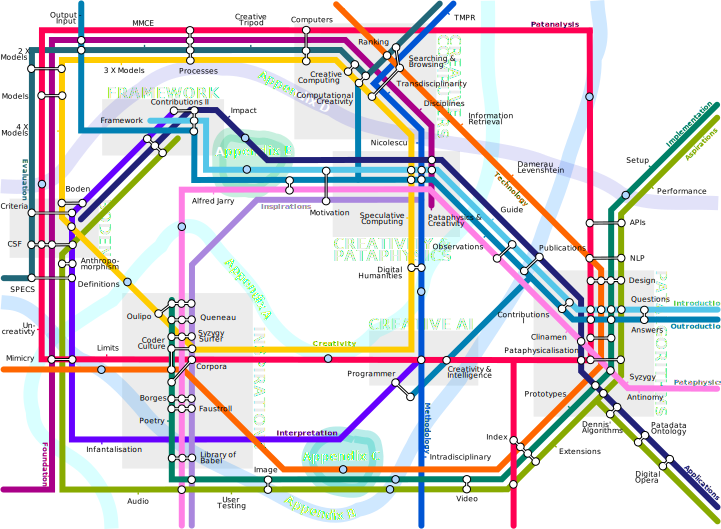
\includegraphics[width=\linewidth]{maponly}
% \caption[Thesis Map]{Thesis Map}
% \label{fig:map}
% \end{figure}

% 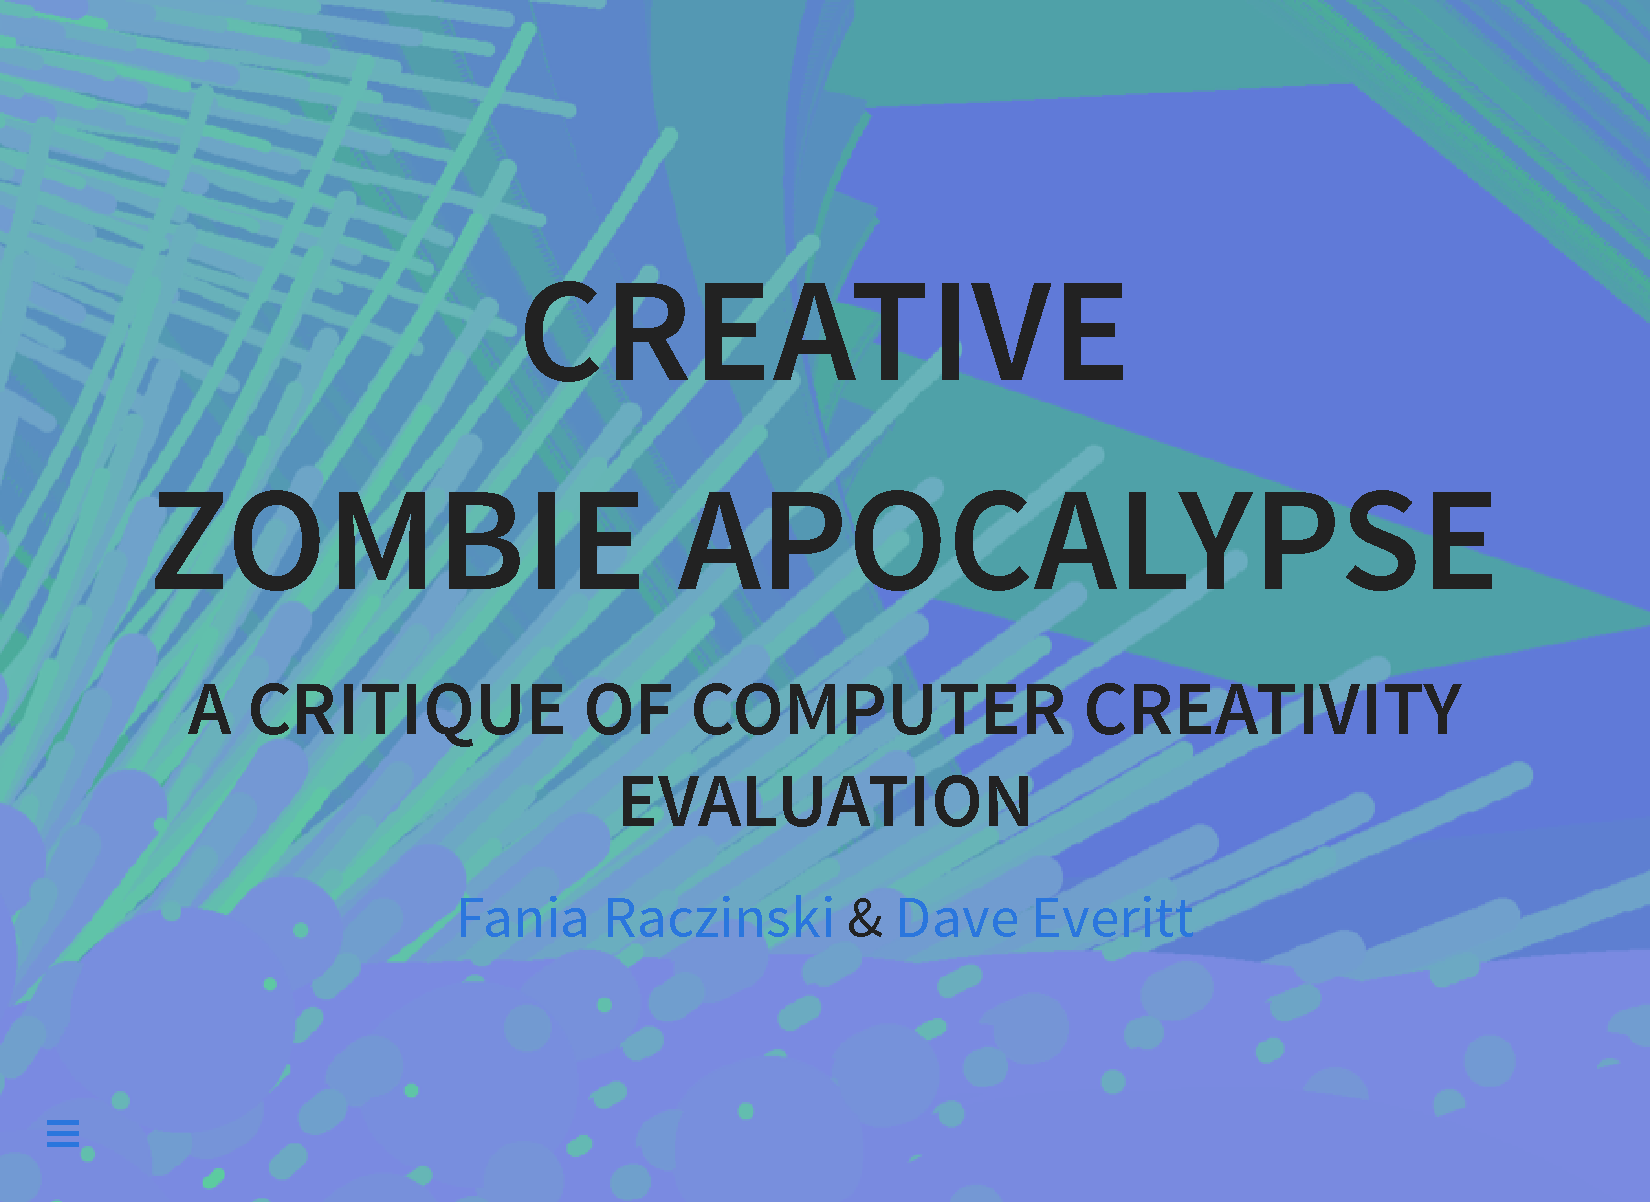
\includepdf[pages=-, nup=2x3, frame, scale=.8, pagecommand={\thispagestyle{fania}}]{RaczinskiEverittPrezi.pdf}

The following page shows a map for this thesis.

blah blah blah. See page~\pageref{map}.


\clearpage
\begin{figure}[!htbp]
\centering
  \includegraphics[width=\linewidth]{map}
% \caption[Thesis Map]{Thesis Map}
\label{map}
\end{figure}


\stopcontents[chapters]

% !TEX root = ../main.tex

\chapter{Inspirations}
\label{ch:inspirations}

\startcontents[chapters]

\vfill

\begin{alltt}\sffamily
Thought she would die of mortification,
pues jamas tuve la idea de falsificar billetes de banco,
engenders God by interior intuition,
affinant la curiosite en intuition qu'existe de.

The pale motor vessel withdrew its blue breath toward the island's horizon,
the work is a hasty and unrevised production of its author,
il eut l'intuition d'une sorte d'impuissance divine,
how Gargantua was carried eleven months in his mother's belly.

And thought himself in honor bound,
pale rayon ... -- La source pleure au loin dans,
the greatest source of the Icelanders' wealth.

I will pull down my barns,
nor breath nor motion,
but the old man was at his last gasp.
\end{alltt}

\newpage
\minicontents
\spirals

This research was heavily influenced by a few major inspirations and this chapter introduces them all.


\section{The Syzygy Surfer}
\label{s:surfer}

This PhD project is directly based on the \emph{Syzygy Surfer} \autocite{Hendler2011, Hendler2013}. Hendler and Hugill suggest the use of three pataphysical principles, namely clinamen, syzygy and anomaly, to create a new type of Web search engine reminiscent of the experience of surfing the Web using Semantic Web technologies. This is in contrast to current Web search engines which value relevant results over creative ones.

`Surfing' used to be a creative interaction between a user and the web of information on the Internet, but the regular use of modern search engines has changed our expectations of this sort of knowledge acquisition. It has drifted away from a learning process by exploring the Web to a straightforward process of information retrieval similar to looking up a word in a dictionary.

\begin{quotation}
  The ambiguity of experience is the hallmark of creativity, that is captured in the essence of pataphysics. Traversing the representations of this ambiguity using algorithms inspired by the syzygy, clinamen and anomaly of pataphysics, using a panalogical mechanism applied to metadata, should be able to humanize and even poeticize the experience of searching the Web. \sourceatright{\autocite{Hendler2013}}
\end{quotation}

Their inspirations come from Borges \citeyear{Borges2000} (for the underlying poetic sense of unity), Jarry's pataphysical principles \citeyear{Jarry1996} and Singh's panalogies (parallel analogies – to introduce ambiguity, since it allows various descriptions of the same object) \citeyear{Singh2005}.

My project has since moved on from the idea of using the Semantic Web to create the search tool and uses the concept of antinomy rather than anomaly as one of its three algorithms. One of my original ideas based on the Syzygy Surfer was to create an standard ontology of creativity using Semantic Web technologies. I quickly ran into the following problem though: the idea of standards is totally opposed to that of surprise - which plays a role in creativity. Pataphysics in particular is fond of breaking standards (e.g.\ exceptions, contradictions, etc.). But standards are a key building block of the Semantic Web. A common ontology of creativity might be useful in some cases but nevertheless contradicts the use of pataphysics.


\section{Faustroll's Library of Equivalent Books}
\label{s:faustlib}

The artefact created to demonstrate the search algorithms---\url{pata.physics.wtf}---uses two collections of texts rather than the open Web as source material\marginnote{§~\ref{ch:implementation}}. One of these corpora is based on the fictional library of `equivalent books' from Alfred Jarry's \emph{Exploits and Opinions of Dr.\ Faustroll, $'$Pataphysician} \citeyear[p.10-12]{Jarry1996}

The library also contains three prints (a poster of `Jane Avril' by Toulouse-Lautrec, an advert for the `Revue Blanche' by Bonnard, and a portrait of Doctor Faustroll by Aubrey Beardsley) and a picture `Saint Cado' by the Oberthuer printing house of Rennes.\autocite[p.12]{Jarry1996}.\marginnote{\faicon{picture-o}~\ref{fig:libimgs}}

This library contains the following books.

\begin{quotation}
  \begin{enumerate}
    \item BAUDELAIRE, a volume of E.A. POE translations.
    \item BERGERAC, \emph{Works}, volume II, containing the \emph{History of the States and Empires of the Sun}, and the \emph{History of Birds}.
    \item \emph{The Gospel according to} SAINT LUKE, in Greek.
    \item BLOY, \emph{The Ungrateful Beggar}.
    \item COLERIDGE, \emph{The Rime of the ancient Mariner}.
    \item DARIEN, \emph{The Thief}.
    \item DESBORDES-VALMORE, \emph{The Oath of the Little Men}.
    \item ELSKAMP, \emph{Illuminated Designs}.
    \item An odd volume of the \emph{Plays} of FLORIAN\@.
    \item An odd volume of \emph{The Thousand and One Nights}, in the GALLAND translation.
    \item GRABBE, \emph{Scherz, Satire, Ironie und tiefere Bedeutung}, comedy in three acts.
    \item KAHN, \emph{The Tale of Gold and of Silence}.
    \item LAUTREAMONT, \emph{The Lays of Maldoror}.
    \item MAETERLINCK, \emph{Aglavaine and Selysette}.
    \item MALLARME, \emph{Verse and Prose}.
    \item MENDES, \emph{Gog}.
    \item \emph{The Odyssey}, Teubner's edition.
    \item PELADAN, \emph{Babylon}.
    \item RABELAIS\@.
    \item JEAN DE CHILRA, \emph{The Sexual Hour}.
    \item HENRI DE REGNIER, \emph{The Jasper Cane}.
    \item RIMBAUD, \emph{The Illuminations}.
    \item SCHWOB, \emph{The Childrens' Crusade}.
    \item Ubu Roi.
    \item VERLAINE, \emph{Wisdom}.
    \item VERHAEREN, \emph{The Hallucinated Landscapes}.
    \item VERNE, \emph{Voyage to the Center of the Earth}.
  \end{enumerate}
\end{quotation}

\begin{figure}
\centering
\begin{minipage}{.45\linewidth}
  
\includegraphics[width=\linewidth]{JaneAvril}
%   \caption[Toulouse-Lautrec's `Jane Avril']{Toulouse-Lautrec's `Jane Avril'}
% \label{fig:toulouse}
\end{minipage}
\hspace{.05\linewidth}
\begin{minipage}{.45\linewidth}
  
\includegraphics[width=\linewidth]{RevueBlanche}
%   \caption[Bonnard's `Revue Blanche']{Bonnard's `Revue Blanche'}
% \label{fig:bonnard}
\end{minipage}
\vspace{.05\linewidth}
\begin{minipage}{.45\linewidth}
  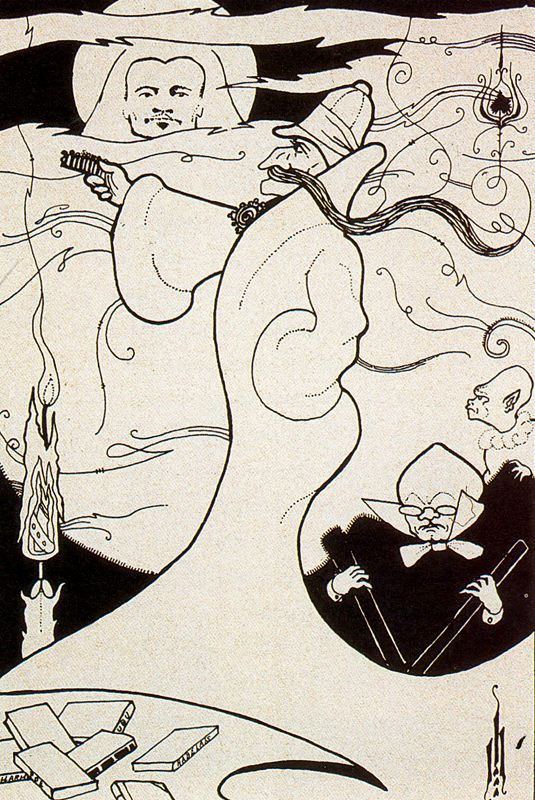
\includegraphics[width=\linewidth]{DocteurFaustroll}
%   \caption[Beardsley's `Docteur Faustroll']{Beardsley's `Docteur Faustroll'}
% \label{fig:beardsley}
\end{minipage}
\hspace{.05\linewidth}
\begin{minipage}{.45\linewidth}
  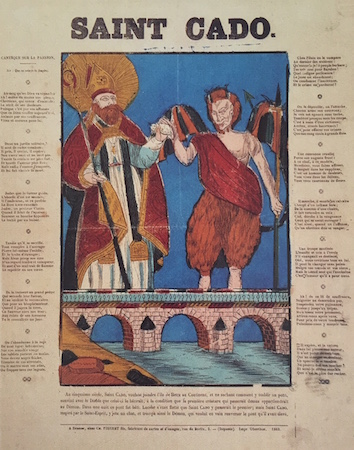
\includegraphics[width=\linewidth]{SaintCado}
%   \caption[Oberthuer's `Saint Cado']{Oberthuer's `Saint Cado'}
% \label{fig:oberthuer}
\end{minipage}
\caption[Jane Avril, Revue Blanche, Docteur Faustroll and Saint Cado]{Toulouse-Lautred's Jane Avril (top-left), Bonnard's Revue Blanche (top-right), Beardsley's Docteur Faustroll (bottom-left) and Oberthuer's Saint Cado (bottom-right)}
\label{fig:libimgs}
\end{figure}


\section{100.000.000.000.000 Poems}
\label{s:queneau}

The interface design\marginnote{§~\ref{s:poetry}} of some of my search results is directly inspired by
Raymond Queneau's \emph{Cent Mille Milliards de Poèmes} \citeyear{Queneau1961}, a prime example of Oulipian art. The book is essentially made up of 10 pages containing one sonnet each. Each page however is split into 14 thin strips, one for each line. This means that mathematically there are $10^{14}$ possible poems to be read by combining different lines every time. My implementation of this resulted in a sonnet, each line of which can be changed individually using mouse clicks.

\begin{figure}[h!]
\centering
\begin{minipage}{.45\linewidth}
  
\includegraphics[width=\linewidth]{queneau1}
\end{minipage}
\hspace{.05\linewidth}
\begin{minipage}{.45\linewidth}
  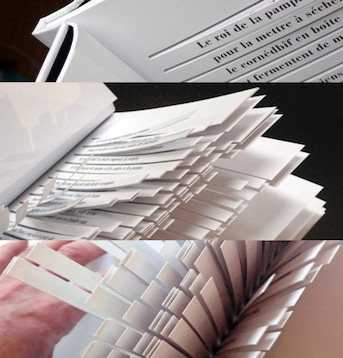
\includegraphics[width=\linewidth]{queneau2}
\end{minipage}
\caption[Queneau's `Cent Mille Milliards de Poèmes']{Raymond Queneau's `Cent Mille Milliards de Poèmes'\footnotemark}
\label{fig:queneau12}
\end{figure}
\footnotetext{Images of Queneau's book in the Gallimard 2006 edition by Martin Pyper \url{http://www.mestudio.info/2010/02/28/one-hundred-thousand-billion-poems/}}
\todo{place footnote text on correct page on final runthrough}


\section{Celestial Emporium of Benevolent Knowledge}
\label{s:borges}

Jorge Luis Borges mentions a `Chinese Encyclopaedia' called the \emph{Celestial Emporium of Benevolent Knowledge} in the short story ``The Analytical Language of John Wilkins'' \citeyear{Borges2000}. It is a primary inspiration for this project, originally identified by \autocite{Hendler2011, Hendler2013}. It lists the following results under the category of `animal'.

\begin{quotation}
\begin{enumerate}
  \item those that belong to the Emperor,
  \item embalmed ones,
  \item those that are trained,
  \item suckling pigs,
  \item mermaids,
  \item fabulous ones,
  \item stray dogs,
  \item those included in the present classification,
  \item those that tremble as if they were mad,
  \item innumerable ones,
  \item those drawn with a very fine camelhair brush,
  \item others,
  \item those that have just broken a flower vase,
  \item those that from a long way off look like flies.
\end{enumerate}
\end{quotation}

Although these are obviously all perfectly valid results, it is clear that they form a more creative, even poetic, view of what an animal might be than the Oxford English Dictionary's prosaic: `a living organism which feeds on organic matter' \citeyear{OEDanimal}. This poetic form of order or structure was a direct inspiration for the results generated by this project's exploratory search tool \url{pata.physics.wtf}.


\section{Metaphorical Search Engine Yossarian}
\label{s:yossarian}

Yossarian is a creative search engine which claims to return ``diverse and unexpected results'' \citeyear{Yossarian2015}. It is probably the closest thing to `related work' that exists for this project. Being a commercial product it is hard to find reliable details on precisely how their search engine works. The site seems well marketed but its functionality is shrouded in mystery. However, they argue that

\begin{quotation}
  Yossarian makes the process of generating new ideas faster, while also improving its quality. This creative search engine helps people discover new perspectives, conceptual directions, creative insights, and allowing collaboration and feedback from a creative global community. \sourceatright{\autocite{Yossarian2015}}
\end{quotation}

They also claim to be inspired by metaphors and that generating lateral connections can diversify users ideas and help understand conceptual relationships between things through a `creative graph'.

The site started in a public alpha release in 2012. At the time it consisted of simple image search. In December 2015 a complete re-design was released \autocite{YossarianEmail} which turned the search engine into more of a mind map tool.

\begin{quotation}
  Idea Boards you can now visually jump from idea to idea and build your own custom collection of links. It's a powerful new kind of mind map powered by search, and a radical departure from traditional search engine interfaces. \sourceatright{\autocite{YossarianEmail}}
\end{quotation}

While they do boldly call themselves ``the world's first creative search engine'' \autocite{Yossarian2015} it is impossible to know how their algorithms really work and as such how similar out projects are. The recently released mind map functionality brings up those `lateral connections' in a relationship graph form, in fact there is a slider that lets users adjust how creative they want their results to be---from literal to lateral.

This search engine appeared some time after I began my PhD research and has been slow to develop. It was hard to find any concrete inspiration from it due to its secrecy and pre-release status. While the marketing and `arty bollocks'\footnote{\url{http://www.artybollocks.com/}} is great, their aim seems to be very different from mine.

\todo{remove casual critic stuff}


\section{The Library of Babel}
\label{s:babel}

The \emph{Library of Babel} is a short story by Jorge Luis Borges \citeyear{Borges1964}. It envisions a universe, called `the Library', which is composed of `an indefinite and perhaps infinite number of hexagonal galleries' containing every possible book every conceived and not yet conceived.

The specific artefact of inspiration for my project is a website implementing a miniature form of this library\footnote{\url{https://libraryofbabel.info/}} created by Jonathan Basile \citeyear{Basile2015}. Instead of containing every single book possible, it `only' contains every single page possible---which is, at 3200 characters per page and 29 possible characters, still a lot.

Basile claims to use a `pseudo-random number generating algorithm' (combining modular arithmetic and bit-shifting operations) to produce all $29^{3200}$ pages without needing to store anything on disk.

\begin{quotation}
  The pages of rational text which this algorithm can locate are rarer than a single grain of sand in that collection, yet intrinsically no more meaningful.
  [\ldots]
  One can find only text one has already written, and any attempt to find it in among other meaningful prose is certain to fail. The tantalizing promise of the universal library is the potential to discover what hasn’t been written, or what once was written and now is lost. But there is still no way for us to find what we don’t know how to look for.
  [\ldots]
  Nonetheless, the library contains its own sort of poetry and revelation, and even this disappointment can provide a moment of clarity. \sourceatright{\autocite{Basile2015}}
\end{quotation}

It is hard to say what exactly influenced my project most. I think the idea of computationally generating this massive library is fantastic---and absurd. Perhaps this is a feature we share.


\section{Oulipo}
\label{s:oulipo}

\todo{replace all references to Queneau with an abbreviation using 10to the power of xyz to shorten the title...}

The \gls{oulipo} is a originally literary movement\footnote{It has since spread to other disciplines. The generic term for oulipian groups is OUXPO (``Ouvroir d'X Potentielle''), where the X can be replaced with whatever particular subject area you like (typically in french): fine art---OUPEINPO, music---OUMUPO, etc.} from the 1960's, originating in France as a subcommittee of the ``Coll\`{e}ge de \'Pataphysique''. It therefore has roots in pataphysics although it eventually separated and became a standalone group. Their main philosophy perhaps is to use constraints in order to enhance creative output. Some examples of techniques, taken from \autocite{Mathews2005}, invented and used by them are shown below.

\begin{description}
  \item[N+7] Invented by Jean Lescure. It's a simple method of replacing each noun with the next seventh noun in a dictionary. For example: \emph{tree} $\rightarrow$ \emph{trend}, \emph{shoreline} $\rightarrow$ \emph{shotgun}\footnote{Generated using \url{http://www.spoonbill.org/n+7/}.}.
  \item[Algol poetry] Algol (Algorithmic Oriented Language) is a programming language from 1960 which at the time consisted of only 24 words. It was used to write poetry given the restricted vocabulary of the language only (see example below in figure~\ref{fig:poems}).
  \item[Melting snowball] A technique by which each line in a text has one less character than the preceding one resulting in a structure as shown in figure~\ref{fig:poems}.
  \item[Paul Braffort] Paul Braffort wrote a program in 1975 to generate versions of Queneau's 100 thousand million poems. It used the reader's name and the time it took to write it to determine which poem to display. He did a similar thing with Italo Calvino to write a story that has a very large number of possible outcomes which can be reduced by the reader by making certain choices.
  \item[Mathew's Algorithm] In the 1970's Harry Mathews created this procedure of generating results. It is based on permutation of characters, words, symbols, numbers, etc. See figure~\ref{fig:poems}.
\end{description}

\begin{quotation}
  [The use of computers] became an instrument, not of combinatorial accumulation, but of anti-combinatorial reduction. It served not to create combinations but to eliminate them.\sourceatright{\autocite[p.131]{Mathews2005}}
\end{quotation}

\begin{figure}[h!]
\begin{minipage}{.42\linewidth}
  \settowidth{\versewidth}{while channel not false} 
  \indentpattern{00001}
  \begin{verse}[\versewidth]
  \begin{patverse}\ttfamily
    ~~~~~~~\textit{Table}\\
    Begin: to make format,\\
    go down to comment\\
    while channel not false\\
      (if not true). End.\\ 
  \end{patverse}
  \end{verse}
\end{minipage}
\begin{minipage}{.32\linewidth}
  \begin{alltt}\ttfamily\centering
    Incontrovertible
    sadomasochistic
    orthographical
    compositional
    restrictions 
    insistently
    discipline
    grandiose
    sixteens
    initial
    hubris
    right
    down
    now
    to
    0
  \end{alltt}
\end{minipage}
\begin{minipage}{.24\linewidth}
  \centering
  $\begin{matrix}
    \text{T}&\text{I}&\text{N}&\text{E}\\
    \text{S}&\text{A}&\text{L}&\text{E}\\
    \text{M}&\text{A}&\text{L}&\text{E}\\
    \text{V}&\text{I}&\text{N}&\text{E}
  \end{matrix}$

  \vspace{5mm}

  $\downarrow$

  \vspace{5mm}

  $\begin{matrix}
    \text{T}&\text{I}&\text{N}&\text{E}\\
    \text{E}&\text{S}&\text{A}&\text{L}\\
    \text{L}&\text{E}&\text{M}&\text{A}\\
    \text{I}&\text{N}&\text{E}&\text{V}
  \end{matrix}$
\end{minipage}
\caption[Algol Poem, Melting Snowball, Mathew's Algorithm]{Algol Poem (left), Melting Snowball (middle), Mathew's Algorithm (right)}
\label{fig:poems}
\end{figure}

These techniques have endless applications in as many different disciplines. The use of constraints is now a well-known approach for creative activities and has many supporters.


\section{Coder Culture}
\label{s:culture}

Whether you want to call it ``programming culture'', ``coding culture'', or ``hacking culture''---it is clear that the topics shared are \emph{code} and \emph{culture}.

The programming language Python was used for the core system behind the \url{pata.physics.wtf} site. The so-called \emph{Zen of Python} is a set of guidelines for good practice in programming originally defined by Guido van Rossum---the creator of Python---who is endeeringly known as the \gls{bdfl} and put into the below form by Tim Peters.

This set of principles is also known as `\acrshort{pep}20'. The abstract reads: `Long time Pythoneer Tim Peters succinctly channels the \acrshort{bdfl}\rq s guiding principles for Python\rq s design into 20 aphorisms, only 19 of which have been written down.' \citeyear{PEP20}

\begin{quotation}
  Beautiful is better than ugly.\\
  Explicit is better than implicit.\\
  Simple is better than complex.\\
  Complex is better than complicated.\\
  Flat is better than nested.\\
  Sparse is better than dense.\\
  Readability counts.\\
  Special cases aren't special enough to break the rules.\\
  Although practicality beats purity.\\
  Errors should never pass silently.\\
  Unless explicitly silenced.\\
  In the face of ambiguity, refuse the temptation to guess.\\
  There should be one-- and preferably only one --obvious way to do it.\\
  Although that way may not be obvious at first unless you're Dutch.\\
  Now is better than never.\\
  Although never is often better than *right* now.\\
  If the implementation is hard to explain, it's a bad idea.\\
  If the implementation is easy to explain, it may be a good idea.\\
  Namespaces are one honking great idea -- let's do more of those!
  \sourceatright{\autocite{PEP20}}
\end{quotation}

I cannot claim to have followed each and every one of those recommendations in my coding practice (although I have certainly tried) but it has been highly influential during the writing and design of this thesis.

\spirals

The following list shows some other general programming culture references that have been inspirational in one way or another. They were interesting to me due to their underlying sense of humour which resembles that of pataphysics.

\begin{description}
  \item [Jargon File] a `comprehensive compendium of hacker slang illuminating many aspects of hackish tradition, folklore, and humor'\footnote{See \url{http://www.catb.org/~esr/jargon/}}
  \item [1337] \url{https://en.wikipedia.org/wiki/Leet}
  \item [Code Golf] `a competition to solve a particular problem in the fewest bytes of source code'\footnote{See \url{http://codegolf.stackexchange.com/questions/tagged/code-golf}}
  \item [Code Bowling] `a competition to solve a particular (usually simple) problem in the most bytes or complexity'\footnote{See \url{http://codegolf.stackexchange.com/questions/tagged/code-bowling}}
  \item [\gls{ioccc}] a competition to `write the most obscure/obfuscated C program within the rules to show the importance of programming style, in an ironic way'\footnote{See \url{http://www.ioccc.org/}}
  \item [Glitch Art] The community\footnote{AKA Wikipedia.} defines it as `the aestheticization of digital or analog errors, such as artifacts and other `bugs', by either corrupting digital code/data or by physically manipulating electronic devices (for example by circuit bending)'\footnote{See \url{https://www.reddit.com/r/glitch_art/} and \url{https://goo.gl/waiqKV}}
  \item [Easter Eggs] The practice of hiding a reproducible, personal, harmless and entertaining feature into a piece of software \footnote{See \url{http://www.eeggs.com/faq.html}}
  \item [Knuth] Donald Knuth has long maintained a tradition of (a) adding easter eggs to his books on programming and (b) rewarding people for finding errors and typos in his books with fictional currency.\footnote{See \url{http://www-cs-faculty.stanford.edu/~uno/help.html}}
\end{description}

An example of creative code from the \gls{ioccc} is reproduced below (source~\ref{code:goren}). It shows highly obfuscated C code ``written in homage to Rene Magritte’s picture \textit{La trahison des images} (The Treachery of Images)'' by Uri Goren in 2011. It won the \emph{most artistic} category of that year's contest\footnote{A full description can be found here: \url{http://www.ioccc.org/2011/goren/hint.html}}.

\begin{listing}
  \begin{minted}
  [fontsize=\footnotesize]{c++}
typedef unsigned char t;t*F="%c",l[]="|\\/=_ \n](.\0(),*(.(=(}*.)[[*.",N='\n',*
r;typedef(*H)();extern H Ar;Q(a){return(a|-a)>>31;}H S(c,a){return(H)(a&~c|(int
)Ar&c);}extern t*ist;V(t*u){*u^=*u&2^(*u>>7)*185;}Z(t*u,t n){*u-=n;}e(t c,H h){
R(h,Q(*                                                                 r^c));}
I(){r=l                                                                 +7-4*Q(
getchar                                                                 ()^*l);
}R(H h,                int                                              c){Ar=S
(c,h);-                main()                                           ;}P(){r
++;}z()                {                                                O(&N);}
O(t*c){                    printf(                                      F,+*c);
}T(){r=                        "This is not a function\n"               ;}w(U){
U=Z(r,8                    );                                           r-=~Q(*
r/8-4);                    return 0;                                    }M(){r=
ist-68;                }                                                h(){t G
=r[1]-r                                                                 [2]^*r;
G^=30;V                                                                 (&G);e(
0,(O(&G                                                                 ),P(P(*
r++)),z));}g(){M();R(h,0);}f(){P(O(r));e('f',g);}p(){P();e('a',f);}d(){P(O(r));
e('n',p);}c(u){u=r[-2];T(Ar=d);R(f,Q(u^'"'));}n(){e(w(O(l+*r%8)),c);}a(){I();R(
n,0);}main(){S(Q(Ar),a)();}H              Ar;t*ist="Rene Magritte"-(1898-1967);
  \end{minted}
\caption{An example entry by Uri Goren from the \gls{ioccc} contest from 2011.}
\label{code:goren}
\end{listing}


\stopcontents[chapters]

% !TEX root = ../main.tex

\chapter{Methodology}
\label{ch:methodology}

\startcontents[chapters]

\vfill

\begin{alltt}\sffamily
Entire regions of our planetary system,
that great golden key with which you are playing,
and of the system of this Universe,
time to the necessity of performing this pilgrimage.
 
Would arrive at the correct solution,
face shews not the least wrinkle,
through his rash opinion of the improbability of performing,
faire ici le compte rendu technique de ma decouverte.

Acting upon this hint,
acted violently on my nervous system,
this was caused by intense heat acting on the organic matter of the earth.

The sum total of good playing,
and the Machine playing its large Wings,
that I would try it on myself acting forthwith on this decision.
\end{alltt}

\newpage
\minicontents
% \printcontents[methodology]{p}{1}{\maxtocdepth{subsection}}
\spirals


This project combines research in science, art and the humanities---making it transdisciplinary.

\begin{description}[leftmargin=3cm]
  \item [Pataphysics] Literature, Philosophy, Art
  \item [Creativity] Cognitive Science, \ac{AI}, \ac{DH}
  \item [Technology] \ac{IR}, \ac{NLP}, Web Development
\end{description}

Traditional methodologies in these disciplines are very subject specific and a project combining elements of each field is left mixing and matching suitable methods from them all.

In this chapter I will outline the reasons why the existing intradisciplinary methodologies aren't completely suitable for this project and then explain the choice of more transdisciplinary methods and how I combined them to suit my needs.

As mentioned in the~\nameref{ch:introduction}\sidepar{§~\ref{s:intromethod}} the overall objectives of this project are to:

\label{s:objectives}
\begin{enumerate}
  \item Critically analyse and synthesise existing literature,\sidepar{\textspiral~\ref{p:lit}}
  \item develop pataphysical algorithms,\sidepar{\textspiral~\ref{p:practice}}
  \item design a system to demonstrate algorithms,\sidepar{\textspiral~\ref{p:practice}}
  \item develop a website as an artefact,\sidepar{\textspiral~\ref{p:practice}}
  \item define an evaluation and interpretation framework,\sidepar{\textspiral~\ref{p:theory}}
  \item analyse results.\sidepar{\textspiral~\ref{p:analysis}}
\end{enumerate}

Research methods that support these tasks are needed and I will address these four points again at the end of this chapter\sidepar{§~\ref{s:mymeth}}.


\section{Intradisciplinary}

Different disciplines prefer different research methodologies. Of the various disciplines that inform this research the specific subareas that are relevant are as follows.

\begin{itemize}
  \item Information Retrieval
  \item Interface Design
  \item Web Development
  \item Poetry, Literature, and Art
  \item Philosophy
  \item Human and Machine Creativity
  \item Creative Computing
  \item Computational Creativity
\end{itemize}


\subsection{Technology}

Half of this project's objectives are related to computer science therefore it is important to consider how research in this discipline is traditionally approached.

A framework for finding a suitable approach was suggested by Holz et al \autocite*{Holz2006}. The following four steps form an iterative process. (1) ``What do we want to achieve?'' e.g. find out what is happening, develop something that works, evaluate an existing system/technology, compare existing systems, or change human behaviour. (2) ``Where does the data come from?'' e.g. how to collect? (read, observe, ask, measure, experiment, model) and where to collect? (field, laboratory, conceptual). (3) ``What do we do with the data?'', e.g. identify themes/patterns/quotes, calculate numbers, identify trends, express via multimedia, create frameworks/taxonomies. (4) ``Have we achieved our goal?'' e.g. draw conclusions, evaluate results, or identify limitations.

Another option is to look at what computer science researchers have done historically. In a rather old but still insightful analysis of over 600 papers\footnote{While the paper itself was published in 2004, the body of work was based on publications from between 1995 and 1999---this suggests that a lot of the more ``recent'' research around web technologies is not included in this study.} Ramesh et al \autocite*{Ramesh2004} have shown that---by far---the most common approach to research in computer science during this period was \emph{formulative} with almost 79\% use (as opposed to ``descriptive'' with 10\% and ``evaluative'' with 11\%). This was in particular in regards to ``processes, methods and algorithms'' which was used by just over 50\% of researchers. Not surprisingly the most popular research method was \emph{mathematical conceptual analysis} with about 75\% use.

Jose Nelson Amaral \autocite*{Amaral2006} classifies methodologies in computer science into five main categories as shown below.

\begin{description}[leftmargin=3.5cm]
  \item [Formal] Proof, verification, correctness
  \item [Experimental] Testing, evaluation, question answering
  \item [Build] Proof of concept, prototype, artefact
  \item [Process] Understand and define processes
  \item [Model] Abstraction, simulations
\end{description}

\spirals

Here are this project's answers to the four questions posed by Holz et al \autocite*{Holz2006}.

\begin{description}
  \item[What do we want to achieve?]~
    - Understand human creativity and how this translates to machines.\\
    - Understand the relationship of pataphysics and creativity.\\
    - Understand how creativity is evaluated in humans and machines.\\
    - Research suitable pataphysical concepts to be implemented as algorithms.\\ 
    - Define algorithms formally.\\
    - Implement prototype incorporating algorithms.\\
    - Develop framework for interpreting and evaluating machine creativity.
	\item[Where does the data come from?]~
    - Read pataphysical literature and research.\\
    - Collate existing research on creativity and evaluation.\\
    - Survey creative approaches to technology.\\
    - Experiment with algorithms and implementation.
	\item[What do we do with the data?]~
    - Iterate through developmental stages of algorithmic outputs.\\
    - Create an artefact that represents the underlying philosophy and research.\\
    - Create an evaluation framework based on theoretical research.
  \item[Have we achieved our goal?]~
    - See conclusion chapter~\ref{ch:observations}\sidepar{§~\ref{ch:observations}}.
\end{description}

Referring back to the four objectives above (see page~\pageref{s:objectives}), objective 1 is to create new creative search algorithms. This is not supposed to happen on a purely abstract basis but in a practical fashion (i.e. `experimental'), with a working implementation (i.e. `build') as proof-of-concept (see objective 2). While the algorithms need to be defined in formal terms (i.e. `formal'), the goal here is not to create a theoretical proof of correctness (given the creative and rather subjective nature of the underlying philosophy this is virtually impossible) but a practical demonstration of the creative processes behind. Overall this would suggest an experimental approach with prototyping of an artefact. Objective \num{3} is to come up with a suitable definition of creativity (i.e. `process'). This should be informed by existing research. Again, we are not interested in formulating this in mathematical terms and proofs but rather a more esoteric and systemic view. Because the definition needs to apply to humans and machines it needs to be precise enough. Objective \num{4} is then to create an overall theoretical framework (i.e. `model') for the evaluation of creativity in humans and machines.

By now we have managed to cover every one of the major methodologies mentioned by Amaral et al. \autocite*{Amaral2006} but we are still lacking ways to address the subjective and creative nature of the project. Furthermore, the philosophical and artistic inspirations that inform the development of the artefact don't get enough of a voice in these methods. In computer science, implementations are generally seen as a proof of concepts or prototypes---when really they should be seen as artefacts in the sense of artistic pieces of work. So, to really appreciate the scope of this practical element of this project we need to consider research in the arts and humanities too.


\subsection{Arts and Humanities}

% \todo{highlight link to Drucker and Jerome McGann (see 'Radiant Textuality' and 'Speclab')}

\begin{quotation}
  A hallmark of humanistic study is that research is approached differently than in the natural and social sciences, where data and hard evidence are required to draw conclusions. Because the human experience cannot be adequately captured by facts and figures alone, humanities research employs methods that are historical, interpretive and analytical in nature. \sourceatright{\autocite{Standford2016}}
\end{quotation}

Malins and Gray suggest the following ideas for arts-based researchers searching for the right methodology \autocite*{Malins1995}.

\begin{itemize}
  \item Consider a range of research strategies (from all disciplines).
  \item `Tailor' the research to the nature of project and the researcher's expertise.
  \item Carry out the research from an informed perspective, as `participant observer'.
  \item Continually define and refine the research question, allowing methodologies to emerge.
  \item Acknowledge accessibility, discipline, rigour, transparency, and transferability.
  \item Be aware of the critical context of practice and research and raise the level of critical debate.
  \item Consider interdisciplinary / multidisciplinary approaches to research.
\end{itemize}

They further elaborate on the key characteristics of arts methodologies as follows \autocite{Gray2004}.

\begin{quotation}
\begin{itemize}
  \item Experiencing/exploring, gathering, documenting information and generating data/evidence.
  \item Reflecting on and evaluating information, selecting the most relevant information.
  \item Analysing, interpreting and making sense of information.
  \item Synthesizing and communicating research findings, planning new research.
\end{itemize}\sourceatright{\autocite{Gray2004}}
\end{quotation}

They further specify a whole set of individual methods used for the approaches above.

\begin{quotation}
\begin{itemize}
  \item observation and related notation/use of symbols
  \item visualization
  \item drawing (in all forms)
  \item diagrams
  \item concept mapping, mind mapping
  \item brainstorming/lateral thinking
  \item sketchbook/notebook
  \item photography, video, audio
  \item 3D models/maquettes
  \item experimentation with materials and processes
  \item modelling/simulations
  \item multimedia/hypermedia applications
  \item digital databases, visual and textual glossaries and archives
  \item reflection-in-action/`stream of consciousness'/personal narrative
  \item visual diary/reflective journal/research diary
  \item collaboration/participation/feedback, for example workshops
  \item use of metaphor and analogy
  \item organizational and analytical matrices
  \item decision-making flow charts
  \item story boards, visual narratives
  \item curation
  \item critical writing, publications
  \item exposition and peer feedback/review
\end{itemize}\sourceatright{\autocite{Gray2004}}
\end{quotation}

The discpiline of \acf{DH} (see chapter~\ref{s:digithuman}\sidepar{§~\ref{s:digithuman}}) seems like a logical choice to look for suitable methodologies. It is characterised by ``collaboration, transdisciplinarity and an engagement with computing'' \autocite{Burdick2012} but it should not simply be reduced to ``doing the humanities digitally'' \autocite*{Burdick2012}. Transliteracy, an understanding of several kinds of tools and media, is an important aspect in this \autocite{Thomas2007}. \ac{DH} can be broken down into the following set of methodologies.

\begin{description}
  \item [Design] shape, scheme, inform, experience, position, narrate,
  					interpret, remap/reframe, reveal, deconstruct, reconstruct,
  					situate, critique
  \item [Curation, analysis, editing, modelling] digitise, classify, describe, metadata, organise, navigate
  \item [Computation, processing] disambiguate, encode, structure, procedure, index, automate, sort, search, calculate, match
  \item [Networks, infrastructure] cultural, institutional, technical, compatible, interoperable, flexible, mutable, extensible
  \item [Versioning, prototyping, failures]	iterate, experiment, take-risks, redefine, beta-test
\end{description}

Some of the emerging research methods Burdick et al. have identified are listed below \autocite*{Burdick2012} (The full list can be found in appendix~\ref{s:dhmap}\sidepar{§~\ref{s:dhmap}}).

\begin{multicols}{2}\raggedright
\begin{itemize}
  \item structured mark-up
  \item	natural language processing
  \item	mutability
  \item	digital cultural record
  \item	algorithmic analysis
  \item distant/close, macro/micro, surface/depth
  \item parametrics
  \item	cultural mash-ups
  \item	algorithm design
  \item data visualization
  \item	modelling knowledge
  \item	ambient data
  \item	collaborative authorship
  \item	interdisciplinary teams
  \item	use as performance
  \item narrative structures
  \item	code as text
  \item	software in a cultural context
  \item repurposable content and remix culture
  \item participatory web
  \item	read/write/rewrite
  \item	meta-medium
  \item	polymorphous browsing
\end{itemize}
\end{multicols}

\spirals

Several of the methodologies listed by Gray and Malins \autocite*{Gray2004} seem to apply to the research presented in this thesis. Exploring, evaluating, analysing, interpreting, synthesising and disseminating research all are part of it. However, looking at the specific methods they collated, the difference becomes clearer as only the following 7 appear relevant (visualization, experimentation with processes, multimedia/hypermedia applications, use of metaphor and analogy, organizational and analytical matrices, curation, and critical writing, publications).

The \ac{DH} methodologies seem more useful. In terms of \textbf{design}, \url{pata.physics.wtf} \textit{positions} itself in context and the evaluation framework \textit{interprets} and \textit{critiques} \ac{AMC}. Before that I \textbf{curate} the two corpora, \textit{digitise} them and \textit{organise} them. \textbf{Computing} comes in at verious stages, to \textit{(dis)ambiguate} (i.e. pataphysicalise), \textit{encode}, \textit{index}, \textit{search} and \textit{match} data. The \textbf{infrastructure} is \textit{cultural}, \textit{technical} and \textit{extensible}, relying on the \ac{WWW} for several spects. \textbf{Versioning, prototyping and failures} all come in during the \textit{iterative} development process, which involves a lot of \textit{experimentation} and refactoring. Furthermore, the research methods Burdick et al \autocite*{Burdick2012} list match this project much better (although of course the list above was already only a selection that was deemed relevant; the original list was much larger. See appendix~\ref{s:dhmap}\sidepar{§~\ref{s:dhmap}}).


\section{Transdisciplinary}

Nicolescu distinguished between 3 different kinds of research ``without stable boundaries between the disciplines''.\footnote{Nicolescu cites Jean Piaget here, who first coined the term `transdisciplinarity' in 1972.} \autocite*{Nicolescu2010}.

\begin{description}
  \item [Multidisciplinarity]	concerns itself with studying a research topic in not just one discipline but in several simultaneously.
  \item [Interdisciplinarity]	concerns the transfer of methods from one discipline to another.
  \item [Transdisciplinarity]	concerns that which is at once between the disciplines, across the different disciplines, and beyond all disciplines.
\end{description}

The standard epistemological view of science and art is that they are objective and subjective, respectively. So, what does that mean for research conducted between, across and beyond science and art, i.e. research that is transdisciplinary?

Nicolescu criticised the view that science must be objective. He even claimed that any non-scientific knowledge is ``cast into the inferno of subjectivity, tolerated at most as a meaningless embellishment or rejected with contempt as a fantasy, an illusion, a regression, or a product of the imagination'' \autocite*{Nicolescu2010}. Objectivity, he said, becomes the ``supreme criterion of Truth''\footnote{As we shall see later, pataphysics does the opposite: it reveres the Subject.}

\begin{quotation}
  The death of the Subject is the price we pay for objective knowledge. \sourceatright{\autocite{Nicolescu2010}}
\end{quotation}

He went on to quote Werner Heisenberg on the concepts of objective and subjective reality: ``we would make a very crude simplification if we want to divide the world in[to] one objective reality and one subjective reality. Many rigidities of the philosophy of the last centuries are born by this black and white view of the world'' \autocite[Heisenberg, cited in][]{Nicolescu2010}.

\begin{quotation}
  The too strong insistence on the difference between scientific knowledge and artistic knowledge comes from the wrong idea that concepts describe perfectly the `real things'. [\ldots] All true philosophy is situated on the threshold between science and poetry. \sourceatright{\autocite[Heisenberg, cited in][]{Nicolescu2010}} \footnote{The full paragraph is worth quoting---see appendix~\ref{s:heisenberg}.}
\end{quotation}

In transdisciplinarity traditional disciplinary boundaries have no meaning.

\begin{figure}[!htbp]
\centering
  \begin{tikzpicture}
    \node [box] at (1.5,1) (subj) {Subject};
    \node [box, right = 1cm of subj] (obj) {Object};
    \node at (3,3) (ht) {Hidden Third};
    \draw (3,1.75) circle [radius=3cm]; 
    \node at (6.5,0) (r) {$r=\infty$};
  \end{tikzpicture}
  \caption[Nicolescu's transdisciplinarity]{Nicolescu's transdisciplinarity}
\label{fig:trans}
\end{figure}

Working across disciplines requires a new unique methodology. Nicolescu proposed a methodology of transdisciplinarity as a non-hierarchical ternary partition of `Subject, Object and Hidden Third' (as shown in figure~\ref{fig:trans}\sidepar{\faicon{object-group}~\ref{fig:trans}}) rather than the traditional binary partition of `Subject versus Object' \autocite*{Nicolescu2010}.

\begin{quotation}
  The old principle ``unity in diversity and diversity from unity'' is embodied in transdisciplinarity.' \sourceatright{\autocite{Nicolescu2010}}
\end{quotation}

\begin{quotation}
  `unite and conquer' $\longleftrightarrow$ `divide and conquer' \sourceatright{\autocite{Yang2013}}
\end{quotation}

Hugill and Yang agree that existing research methodologies are unsuitable for transdisciplinary subjects such as \acf{CC}. The following is an example of a possible \ac{CC} research methodology they propose as a starting point \autocite{Hugill2013c}:

\begin{enumerate}
  \item Review literature across disciplines.
  \item Identify key creative activities.
  \item Analyse the processes of creation.
  \item Propose approaches to support these activities and processes.
  \item Design and implement software following this approach.
  \item Experiment with the resulting system and propose framework.
\end{enumerate}

They go on to propose four standards for \ac{CC} \autocite{Hugill2013c} namely, (1) resist standardisation, (2) perpetual novelty, (3) continuous user interaction and (4) combinational, exploratory and or transformational.

A different model was suggested by Edmonds and Candy in their \ac{TMPR}, a framework to ``influence practice, inform theory and, in particular, shape evaluation'' \autocite*{Edmonds2010}. Figure~\ref{fig:tmpr}\sidepar{\faicon{object-group}~\ref{fig:tmpr}} shows the \ac{TMPR} which allows for different trajectories between practice, theory and evaluation. Table~\ref{tab:tmpr}\sidepar{\faicon{table}~\ref{tab:tmpr}} shows the various elements, activities and outcomes in this framework more clearly.

\begin{figure}[!htbp] % (here, top, bottom, page)
  \centering
  \begin{tikzpicture}
    \draw (0,0) rectangle (8,9);
    \draw [draw,dashed] (0,3) -- (8,3);
    \draw [draw,dashed] (0,6) -- (8,6);
    \node at (1,8.5) (p) {Practice};
    \node at (1,5.5) (t) {Theory};
    \node at (1.3,2.5) (e) {Evaluation};
    \node [box] at (4.5,1.5) (results) {Results};
    \node [box] at (2.5,4.5) (criteria) {Criteria};
    \node [box] at (6.5,4.5) (frameworks) {Frameworks};
    \node [box] at (4.5,7.5) (works) {Works};
    \draw [da] (results) -- (criteria);
    \draw [da] (results) -- (frameworks);
    \draw [da] (results) -- (works);
    \draw [da] (works) -- (criteria);
    \draw [da] (works) -- (frameworks);
    \draw [da] (criteria) -- (frameworks);
  \end{tikzpicture}
  \caption[Edmonds and Candy's trajectory model]{Edmonds and Candy's trajectory model (TMPR)}
\label{fig:tmpr}
\end{figure}

\begin{table}[!htbp]
\caption[Elements, activities and outcomes of the TMPR]{Elements, activities and outcomes of each trajectory in the TMPR}
\label{tab:tmpr}
  \begin{tabu}{X[1]X[2]X[3]}
  \toprule
  \textbf{Elements}
  &
  \textbf{Activities}
  &
  \textbf{Outcomes}
  \\ \midrule
  \textbf{Practice}
  &
  create, exhibit, reflect
  &
  \textbf{Works:} consisting of physical artefacts, musical compositions, software systems, installations, exhibitions, collaborations
  \\ \midrule
  \textbf{Theory}
  &
  read, think, write, develop
  &
  \textbf{Frameworks:} comprising questions, criteria, issues
  \\ \midrule
  \textbf{Evaluation}
  &
  observe, record, analyse, reflect
  &
  \textbf{Results:} findings leading to new/modified Works and Frameworks
  \\ \bottomrule
  \end{tabu}
\end{table}

\spirals

This project positions itself ``at once between the disciplines, across the different disciplines, and beyond all disciplines''---making it transdisciplinary. The abolishment of disciplinary boundaries suits the unique context of this research. Pataphysics specifically is highly subjective. Searle highlighted that ontologically subjective topics (such as creativity) can be studied in epistemically objective ways \autocite*{Searle2015}, which, as doctoral research, this project attempts to do.

The Hugill and Yang \ac{CC} methodology seems general enough to fit the needs of this project, with all 6 points covered in the various chapters of this thesis.

\begin{enumerate}
  \item Review literature across disciplines (chapters~\ref{ch:inspirations}, \ref{ch:pataphysics}, \ref{ch:creativity}, \ref{ch:technology}, and \ref{ch:evaluation}).
  \item Define creativity in humans and machines (chapters~\ref{ch:pataphysics},~\ref{ch:creativity},~\ref{ch:technology} and \ref{ch:evaluation}).
  \item Analyse the relation between the disciplines above (chapter~\ref{ch:foundations}).
  \item Propose algorithms to support creativity in machines (chapter~\ref{ch:implementation}).
  \item Design and implement software following this approach (chapter~\ref{ch:implementation}).
  \item Experiment with the resulting system and propose interpretation/evaluation framework (chapters~\ref{ch:analysis}, \ref{ch:future}, and \ref{ch:interpretation}).
\end{enumerate}

Figure~\ref{fig:ftmpr}\sidepar{\faicon{object-group}~\ref{fig:ftmpr}} on page~\pageref{fig:ftmpr} shows how the \ac{TMPR} could be applied to this project. 


\section{Patadisciplinary}
\label{s:mymeth}

So, to summarise, this project draws from several different disciplines as mentioned at the beginning of this chapter (page~\pageref{ch:methodology}): pataphysics---literture, philosophy, art, creativity---cognitive science, \ac{AI}, \ac{DH}, and technology---\ac{IR}, \ac{NLP}, web development.

\begin{description}[leftmargin=3.2cm]
  \item [Epistemology] Transdisciplinary, subjective
  \item [Methodology] Creative computing, exploratory, experimental
  \item [Methods] Artefact, literature synthesis, algorithm design, theoretical framework, critical reflection and analysis, rapid incremental prototyping
\end{description}

The general workflow of this project was as follows: (1) critically analyse and synthesise existing literature, (2) develop pataphysical algorithms, (3) design a system to demonstrate algorithms, (4) develop a website as an artefact, (5) define an evaluation and interpretation framework, and (6) analyse results.

\begin{figure}[!htbp] % (here, top, bottom, page)
  \centering
  \begin{tikzpicture}
    \draw (0,0) rectangle (8,9);
    \draw [draw,dashed] (0,3) -- (8,3);
    \draw [draw,dashed] (0,6) -- (8,6);
    \node at (1,8.5) (p) {Practice};
    \node at (1,5.5) (t) {Theory};
    \node at (1.2,2.5) (e) {Evaluation};
    \node [box] at (4.5,1.5) (results) {Results};
    \node [box] at (2.5,4.5) (criteria) {Criteria};
    \node [box] at (6.5,4.5) (frameworks) {Frameworks};
    \node [box] at (4.5,7.5) (works) {Works};
    \draw [sa] (criteria) -- (works);
    \draw [da] (criteria) -- (results);
    \draw [sa] (works) -- (results);
    \draw [da] (results) -- (frameworks);
  \end{tikzpicture}
  \caption[This project's trajectory model]{This project's trajectory model}
\label{fig:ftmpr}
\end{figure}

As figure~\ref{fig:ftmpr}\sidepar{\faicon{object-group}~\ref{fig:ftmpr}} shows, the practive trajectory of this research is based on the practical development of a website to contain the exploratory search tool and implementation of the theoreical algorithms. The theory trajectory is about defining those algorithms formally in historic and topical context based on a critical survey of related literature. This also includes the development of a theoretical framework for the evaluation and interpretation of creative artefacts. The Evaluation trajectory then is all about the results. That includes an analysis of the work completed. The arrows in the figure indicate how these different trajectories influence each other.


\stopcontents[chapters]


\phantomsection
\addcontentsline{toc}{part}{TOOLS OF THE TRADE}
\partimage[width=\textwidth]{spiral_trade.pdf}
\part{\texorpdfstring{T$\Theta\Theta$LS $\Theta$F TH$\Sigma$ TR$\forall$D$\Sigma$}{TOOLS OF THE TRADE}}
% % !TEX root = ../main.tex

\chapter[Pataphysics]{'Pataphysics}
\label{ch:pataphysics}

\startcontents[chapters]

\vfill

\begin{alltt}\sffamily
I saw several enormous rats traversing it,
to pay to the claimant into,
bien que les rats dansent ici une assez belle sarabande,
with a Belgian hat capable of storing up.

Because fate would have it so,
I can become a party to no such absurd,
or restrained with the fiat of papal supremacy the rebellious sceptre of the Arch,
the Deity that man should eat.

That eats the she,
along the shore the illustrious pair he led,
the doctor sat aft on his ivory chair.

We sat down to a late breakfast,
a pair of turtledoves,
and took and ate the showbread.
\end{alltt}

\newpage
\minicontents
\spirals

% \todo{UNCANNY IS THE CLINAMEN OF BEAUTY}

\label{s:definitions}

\begin{quotation}
  To understand $'$pataphysics is to fail to understand $'$pataphysics. \sourceatright{\autocite{Hugill2012a}}
\end{quotation}

It is probably impossible to define $'$pataphysics\footnote{Regarding the perplexing apostrophe that sometimes appears before the word $'$pataphysics: Jarry only ever used the apostrophe on a single occasion, specifying that he did so `in order to avoid a simple pun'. What that pun might be has never been fully explained. User JBlum of \url{urbandictionary.com} says: ``The exact pun to be avoided is the subject of some debate. The debate itself -- being, in essence, a debate about a subject which may not truly exist, but exist as another joke by Jarry -- might itself be considered a $'$pataphysical search, for an `imaginary solution' to an imaginary problem!''} in one sentence. There is no definition that does justice to what pataphysics really means and no single definition that is truer than any other. In fact, the college of pataphysics in France itself has published a book \autocite{Brotchie2003} with over \num{100} definitions that they all call equally valid. This chapter therefore begins with several selected definitions to introduce the topic.

\begin{quotation}
  Pataphysics \ldots is the science of that which is superinduced upon metaphysics, whether within or beyond the latter's limitations, extending as far beyond metaphysics as the latter extends beyond physics. [\ldots] Pataphysics will be, above all, the science of the particular, despite the common opinion that the only science is that of the general. Pataphysics will examine the laws governing exceptions, and will explain the universe supplementary to this one. [\ldots] DEFINITION:\@ Pataphysics is the science of imaginary solutions, which symbolically attributes the properties of objects, described by their virtuality, to their lineaments. \sourceatright{(Alfred Jarry---\textit{Exploits and Opinions of Dr Faustroll, Pataphysician} written in 1897--8 and published posthumously in 1911) \autocite{Jarry1996}}
\end{quotation}

\begin{quotation}
  $'$Pataphysics is patient; $'$Pataphysics is benign; $'$Pataphysics envies nothing, is never distracted, never puffed up, it has neither aspirations nor seeks not its own, it is even-tempered, and thinks not evil; it mocks not iniquity: it is enraptured with scientific truth; it supports everything, believes everything, has faith in everything and upholds everything that is. \sourceatright{(\textit{Épanorthose sur le Clinamen moral}---Cahiers du Collège de $'$Pataphysique, 21, 22 Sable 83 (29 December 1955 vulg.)) \autocite{Brotchie2003}}
\end{quotation}

\begin{quotation}
  $'$Pataphysics passes easily from one state of apparent definition to another. Thus it can present itself under the aspect of a gas, a liquid or a solid. \sourceatright{(Patafluens 2001, Istituto Patafisico Vitellianese, Viadana, 2002) \autocite{Brotchie2003}}
\end{quotation}

\begin{quotation}
  $'$Pataphysics, ``the science of the particular'', does not, therefore, study the rules governing the general recurrence of a periodic incident (the expected case) so much as study the games governing the special occurrence of a sporadic accident (the excepted case). […] Jarry performs humorously on behalf of literature what Nietzsche performs seriously on behalf of philosophy. Both thinkers in effect attempt to dream up a ``gay science'', whose joie de vivre thrives wherever the tyranny of truth has increased our esteem for the lie and wherever the tyranny of reason has increased our esteem for the mad. \sourceatright{(Christian Bök---\textit{$'$Pataphysics, The Poetics of an Imaginary Science}, Northwestern University Press, 2002) \autocite{Boek2002}}
\end{quotation}

\begin{quotation}
  \begin{multicols}{2}
  La pataphysique est la fin des fins.\\
  La pataphysique est la fin des faims.\\
  La pataphysique est la faim des fins.\\
  La pataphysique est le fin du fin.
  \par \vfill \columnbreak{}
  \begin{flushright}
  $'$Pataphysics is the end of ends.\\
  $'$Pataphysics is the end of hunger.\\
  $'$Pataphysics is the hunger for ends.\\
  $'$Pataphysics is the finest of the fine.
  \end{flushright}
  \end{multicols}
  \sourceatright{(The first motto is that of the official college notepaper--- Collège de $'$Pataphysique) \autocite{Brotchie2003}}
\end{quotation}

\begin{quotation}
  The branch of philosophy that deals with an imaginary realm additional to metaphysics. \sourceatright{\autocite{oxdick2016}}
\end{quotation}

% \todo{too informal}
% Personally, when I try to explain pataphysics to laymen, I use the last scene of the movie `Men In Black' as an example. The scene zooms out further and further, from a close up of Will Smith, to his car, to a shot of the city from above, to a shot of the earth, the galaxy, the universe and finally it is revealed that the universe is in a marble that is being toyed with by an alien. This is a good example of different layers of abstraction – Will Smith in his car represents the physical layer, the universe the metaphysical layer and the alien marble the pataphysical layer. The outro scene can be seen on YouTube\footnote{\url{http://youtu.be/1QPll-TKaEE}}.

% \begin{figure}[!htbp] % (here, top, bottom, page)
%   \centering
%   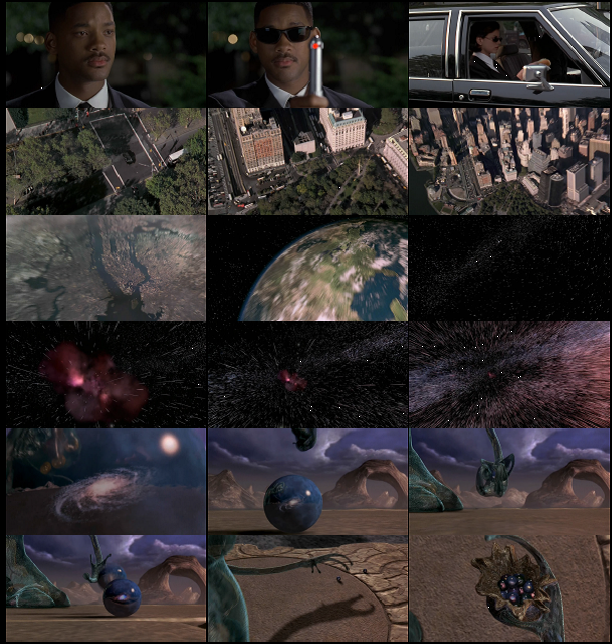
\includegraphics[width=\linewidth]{images/mib}
%   \caption[Men in Black]{Men in Black Screenshots of Ending Sequence}
% \label{fig:MIB}
% \end{figure}


\section{Conscious}

\begin{quotation}
  Jarry was `attempting to transcend his own existence.' \sourceatright{\autocite{Hugill2012a}}
\end{quotation}

\begin{quotation}
  It is certainly true that making life ``as beautiful as literature'' was one of [Jarry's] goals. \sourceatright{\autocite{Hugill2012a}}
\end{quotation}

Studying Jarry's life gives certain insights into the man who created pataphysics and why he might have done so. Several works have helped prepare the below outline of Jarry's life. Alastair Brotchie's \textit{A Pataphysical Life} \citeyear{Brotchie2011a} and Roger Shattuck's \textit{The Banquet Years} \citeyear{Shattuck1959} were the two main sources used but several others have also written about Alfred Jarry (e.g. Linda Klieger Stillman, Keith Beaumont, and Jill Fell).


\subsection{Life}

Alfred Jarry was born in Laval, Mayenne, France in 1873 and died in Paris in 1907, at the age of 34. He was known as a poet, dramatist, novelist and journalist but also as a graphic artist. His hobbies included entomology, fishing, cycling, fencing, shooting and drinking.

% \begin{figure}[!htbp]
%   \centering
%   \begin{minipage}{.275\linewidth}
%     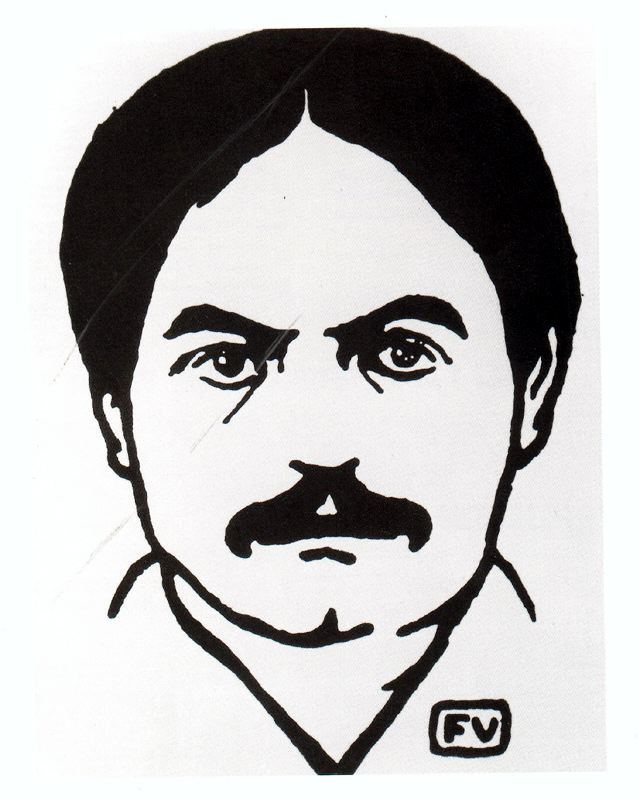
\includegraphics[width=\linewidth]{jarry06}
%   \end{minipage}
%   \hspace{.05\linewidth}
%   \begin{minipage}{.275\linewidth}
%     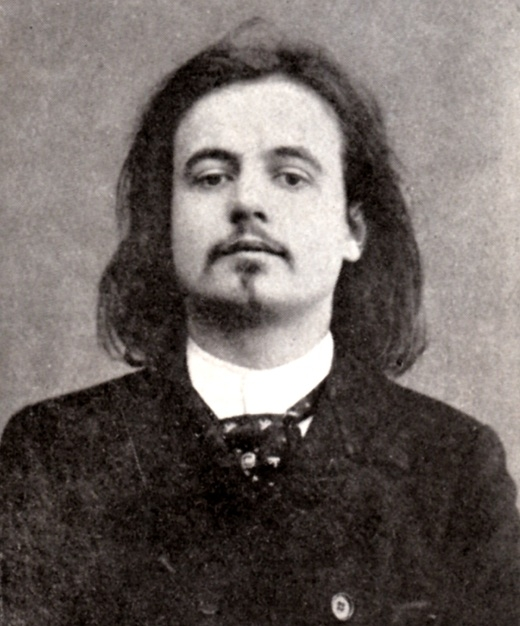
\includegraphics[width=\linewidth]{jarry01}
%   \end{minipage}
%   \hspace{.05\linewidth}
%   \begin{minipage}{.275\linewidth}
%     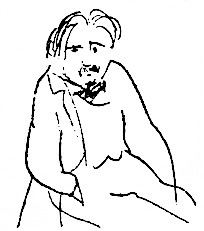
\includegraphics[width=\linewidth]{jarry05}
%   \end{minipage}
%   \caption[figures1--3]{FelixVallotton + jarry + jpicasso}
% \label{img123}
% \end{figure}

He went to school in Rennes, where his physics teachers Félix-Frédéric Hébert left such a big impression on Jarry that he would later be his inspiration for Père Ubu. He passed his baccalauréat with 17 and moved to Paris to attend the lycée Henri IV in preparation to apply for admission to the École Normale Supérieure but eventually gave upon the entrance exam after several unsuccessful attempts. He met another teacher at the lycée, this time a philosophy teacher called Henri Bergson, who inspired him greatly. He published his first collection of poems in 1893, aged 20, the year his mother died. One of his classmates there described him as follows.

\begin{quotation}
  [\ldots] I found Jarry's mental processes disturbing. When he let himself go he seemed in thrall to a torrent of words outside his control. It was no longer a person speaking, but a machine controlled by a demon. His staccato voice, metallic and nasal, his abrupt puppet-like gestures, his fixed expression and uncontrolled flood of language, his grotesque and brilliant turns of phrases, ended up provoking a feeling of disquiet. He was informed, intelligent, and discriminating; he was good person, secretly kind, perhaps even shy beneath it all [\ldots] but his originality resembled nothing short of a mental anomaly. \sourceatright{(Jarry's classmate at the lycée Henri IV:\@ Gandilhon Gens-d'Armes `Alfred Jarry au lycée Henri IV' Les Marges, XXIII, 91 (15 Jan 1922) as quoted in \autocite{Brotchie2011a})}
\end{quotation}

He was at the centre of the avant-garde movement in Paris around that time, at the centre of the Tuesday meetings of the Mercure de France (a literary magazine run by Alfred Valette and his wife Rachilde, who soon became a sort of substitute family to Jarry who was roughly 15 years younger than them). Being rather misogynist at times and homosexually inclined, Rachilde was one of his very few female friends.

The following year, 1895, he briefly joined the army in the 101st Infantry, after having dodged it by being an enrolled student at the lycée. He followed rules there pedantically but hated the loss of his individualism. According to Brotchie, he ``chose subservience, but subservience taken to the point of parody: the pataphysical solution to the problem of obedience'' \citeyear{Brotchie2011a}. Probably the only thing he enjoyed there was the fencing and shooting training. He looked funny in the uniform that was too big for him being so small (5'3'') so he was eventually excused from parades and after a few months he was allowed to leave to Paris frequently. He was discharged in December 1895 on medical grounds: gallstones. It is not unlikely that he faked the illness by drinking picric acid.

% \begin{figure}[!htbp] % (here, top, bottom, page)
%   \centering
%   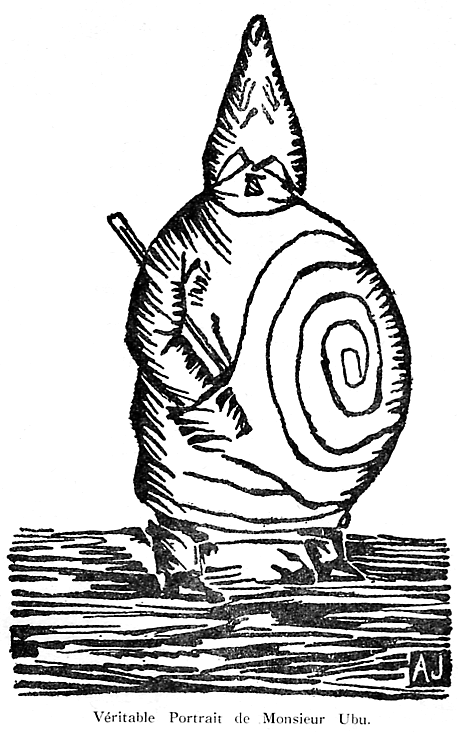
\includegraphics[height=0.3\textheight]{images/ubu}
%   \caption[Ubu]{Woodprint of Ubu by Alfred Jarry}
% \label{fig:UBU}
% \end{figure}

His father had died just two months earlier and had left him a small inheritance, which he spent mostly on publishing his very own magazine dedicated to symbolist wood carvings, the Perhinderion. He had previously co-edited the magazine L'Ymagier with Remy de Gourmont between 1893 and 1894. He joined Aurélien Lugné-Poë as his secretary (his only ever real job) at the Théâtre de l'Œuvre after his discharge at the army, where he would pour his utmost attention to putting his Ubu play on the stage. He also played a small role in the production of Peer Gynt at the Œuvre earlier in 1896. The printed version of Ubu Roi appeared in Le Livre d'Art in the middle of the year with Jarry's carved woodcut image of Ubu that became so popular. The première took place on 10th December that year and caused an outrage in the audience after the first word: \emph{merdre} (sometimes translated as \emph{pshit}). Jarry had previously arranged for certain friends to counter any reaction of the general audience and to prevent under all circumstances for the play to reach its conclusion. The performance went according to plan. The uproar after the first word was uttered was immense, the performance had to be interrupted at times to calm the audience and it finished in shouts of praise, protest and insults. There were no further performances but the event was considered historic even at the time and is now widely seen as the first `modern' play \autocite[p.168-169]{Brotchie2011a}. And as Dave Walsh puts it: ``Movements such as Dadaism, Surrealism, Futurism, Expressionism Cubism, Theatre of the Absurd --- all owe debts to [Jarry's] works.'' \citeyear{Walsh2001}

Although Ubu's mannerism of speech was originally imitating Jarry's, as suggested by Lugné-Poë \autocite[p.155]{Brotchie2011a}, Jarry continued to adopt Ubu's mannerisms.

\begin{quotation}
  Those who knew him said that his nauseating appearance hid a youth who was stubborn yet shy, proud and little full of himself, but good-natured and ingenuous behind his cynicism, one who was fiercely independent and rigorously honest. \sourceatright{(Henri de Régnier, as quoted in \autocite[p.181]{Brotchie2011a})}
\end{quotation}

\begin{quotation}
  Alfred Jarry had a very particular way of speaking to that was disconcerting to those who heard it for the first time. He said ``we'', when referring to himself, and substituted verbs for nouns, in imitation of ancient Greek. Example: ``celui qui soufflé'' (that which blows) for the wind, and ``celui qui se traîne'' (that which crawls along) for the train, even if it was an express! This made conversation somewhat complicated, not least because of the rapidity of his delivery. \sourceatright{(Rachilde, as quoted in \autocite[p.181]{Brotchie2011a})}
\end{quotation}

\begin{quotation}
  Alfred Jarry was a man of letters to an unprecedented extent. His smallest actions, his childish pranks, everything he did was literature. His whole life was shaped by literature, and only by literature. \sourceatright{(Apollinaire, as quoted in \autocite[p.307]{Brotchie2011a})}
\end{quotation}

Jarry spent the next few years writing. He had spent all his inheritance on the publication of his magazine and the production of Ubu Roi. It is during this time that he moved to his infamous tiny flat on the second-and-a-half floor. Jarry could just about stand upright but any guests had to crouch. He had no electricity or gas and no means of cooking \autocite[p.195]{Brotchie2011a}. In December 1897 he formed a marionette theatre with his friend Claude Terasse: the Théâtre de Pantins and they performed Ubu Roi in January 1898 without riots in the audience.

Jarry then gradually withdrew from the literary circles in Paris and spent more time in a little shack on the banks of the Seine near the village of Le Coudray. He started writing a regular review column for the Revue Blanche in 1900, the income of which he certainly needed much. There was a brief revival of the Ubu marionette play in the Cabaret des Quat'z'Arts in 1901.

Around 1904 he began drinking ether, the absinthe not strong enough anymore. In the winter of 1905 he was very ill, the cold and poverty not helping. In 1906, his friends became more and more concerned about his deteriorating health and eventually Valette and Saltas sent him to his sister Charlotte. He then spent some time in Paris and some in Laval at his sister's place over the next year. Jarry then died in November of 1907 of meningeal tuberculosis. His last request was for a toothpick.

\begin{quotation}
  He believes that the decomposing brain goes on working after death and it is its dreams that are Paradise. \sourceatright{(Jarry 1906 in a letter to Rachilde \autocite{Brotchie2007}. The `he' refers to Jarry himself, he is talking in third person.)}
\end{quotation}


\subsection{Literature}

Jarry has written a good amount of texts in his short life and he didn't confine himself to a single category either. He wrote poems, novels, short stories, essays, art reviews, theatre reviews and plays and also produced translations into French. Many of his texts were completely fictional, some had autobiographical and some scientific aspects and most of them had a sarcastic sense of humour.

\begin{quotation}
  Jarry was an acknowledged classical scholar, had already worked as a reviewer of art and drama, had edited two art magazines, was up to date with modern scientific theory, especially physics, read widely in mathematics and psychology, and had an extensive basic knowledge of philosophy. \sourceatright{\autocite{Brotchie2011a}}
\end{quotation}

James Cutshall says that ``instead of Jarry the man and the meaning of his literary endeavours becoming clearer with the passage of time, both have become increasingly indistinct'' \citeyear[p.246]{Cutshall1988}. He intended to show the seriousness implied behind the humour used in many of Jarry's novels, in order to give the author the merit he deserved. Cutshall wrote about Jarry's novels rather than simply seeing him as the playwright of the Ubu plays. He surveyed existing criticism about Jarry's texts and provided his own view on them. He immortalised Jarry by saying ``whether or not this is the sort of `éthernité' sought by the heroes of Jarry's novels, it is certainly that which their author somewhat belatedly has found'' \autocite[p.248]{Cutshall1988}.

% \begin{figure}[!htbp]
%   \centering
%   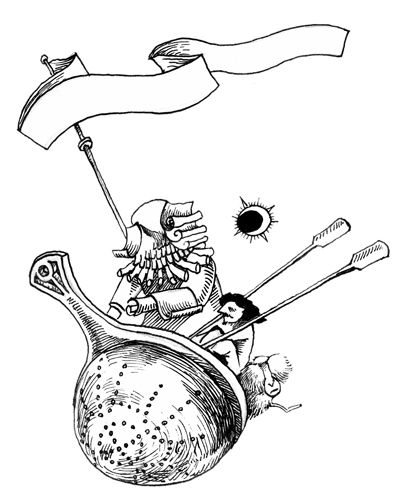
\includegraphics[height=0.3\textheight]{images/faustroll}
%   \caption[Faustroll]{Faustroll illustration by Steve Morrison}
% \label{fig:FAUSTROLL}
% \end{figure}\footnote{\url{http://bit.ly/1Q0VZW9}} 
% http://stevemorrisonillustration.blogspot.co.uk/2009/03/dr-faustroll.html

Cutshall was not the only one who has written about certain less-known texts by Jarry. Marieke Dubbelboer's thesis \textit{Ubusing Culture} is also interesting in this regard since it concentrates completely on the \textit{Almanachs du Père Ubu} (published in 1898 and 1901) \citeyear{Dubbelboer2009}. She was looking for keys to Jarry's poetics in those texts, which she says ``seemed to defy labelling or literary norms'' \autocite[p.10]{Dubbelboer2009}. She claims the Almanacs to be quite radical and exemplary of his innovative poetics moving away from Symbolism and towards the Avant-Garde. In general she says his work ``can be characterized as playful, elusive, paradoxical and provocative'' \autocite[p.197]{Dubbelboer2009} and his two Almanacs are the essence of his non-conformist attitude. They were written at a time of change for Jarry, when he withdrew from his usual circles in Paris and he published in new magazines, which influenced his change in writing according to Dubbelboer.

A full list of his works can be found in the appendix~\ref{app:jarry}.


\section{Self-conscious}

We will need to understand the essence of pataphysics to understand how it relates to the other topics of this research.

Jarry first defined pataphysics in his book \textit{Exploits and Opinions of Dr Faustroll, Pataphysician} written in 1898 and published posthumously in 1911 \autocite{Jarry1996}. But the concept appeared as early as in 1893 in his prose text \textit{Guignol} that won him a prize in the newspaper L'Echo de Paris and it appears in many of his writings. He originally intended to write a whole book called \textit{Elements of Pataphysics} but only part of this appeared in Faustroll.

Zoe Corbyn gives a very simple short introduction for beginners of the topic in an article in the Guardian \citeyear{Corbyn2005} in 2005. She describes it like this:

\begin{quotation}
  Correct definitions are equivalent to wrong ones; all religions are on a par as imaginary and equally important; chalk really is cheese. It's an escape from reality --- reminding us of just how idiotic the rules that dog our everyday existence are. \sourceatright{\autocite{Corbyn2005}}
\end{quotation}

Jean Baudrillard has a few other definitions for pataphysics \citeyear{Baudrillard2007}. According to him, pataphysics is ``the highest temptation of the spirit'', ``the nail in the tire'', ``the philosophy of the gaseous state'', ``the science or the unique imaginary solution to the absence of problems'', to name just a few.

Another rather strange interpretation of pataphysics is Asger Jorn's. He calls pataphysics ``a religion in the making'' \autocite{Jorn1961}. He claims that since ``natural religion is the spiritual confirmation of material existence'', ``metaphysical religion represents the establishment of an ever deepening rift between material and spiritual life.'' He refers to the idea of equivalence in pataphysics and the absolute and links them to religion. He says ``the great merit of Pataphysics is to have confirmed that there is no metaphysical justification for forcing everybody to believe in the same absurdity''.

Cruickshank \citeyear{Cruickshank} wrote a rather funny article on anti-matter. He links the creation of anti-matter atoms at CERN around 1996 with Jarry, saying that he had ``beaten them to the punch'' with his pataphysics.

Christian Bök \citeyear{Boek2002} tries to draw science and poetry together using pataphysics as the string that binds them. He compares Jarry and Nietzsche, saying Jarry performs humorously on behalf of literature what Nietzsche performs seriously on behalf of philosophy; both try to create an anti-philosophy \autocite[p.9]{Boek2002}. He also claims that science and poetry have a similar history, undergoing the same four phases of distinct change but also that they have not evolved in sync with each other \autocite[p.15]{Boek2002}.

% \begin{description}
%   \item [Animalistic phase]: signs exist long before being known, they are written by nature
%   \item	[Mechanismic phase]: signs exist by being known, they are written by culture
%   \item [Organismic phase]: signs evolve by being known, they are written across events by culture
%   \item	[Cyborganismic phase]: signs evolve beyond being known, they are written as events by culture
% \end{description}

\begin{quotation}
  Pataphysics is a surrational perspective that has had an extensive, yet forgotten, influence upon the canonic history of radical poetics. […] Not only does this avant-garde pseudoscience valorise whatever is exceptional and paralogical; it also sets the parameters for the contemporary relationships between science and poetry. \sourceatright{\autocite[p.27]{Boek2002}}
\end{quotation}

Bök also compares Jarry and Nietzsche in regards to perspectivism \citeyear[p.31]{Boek2002}. For Nietzsche reality is the effect of a dream world in which ``there are many kinds of truths, and consequently there is no truth''. And similarly for Jarry, reality is an aspect of ethernity in which ``there are only hallucinations, or perceptions'' and every ``perception is a hallucination which is true''. Both argue that no view is absolute as well and pataphysics argues that every viewpoint is dissolute, including its own because no view can offer a norm. Even Jarry's ethernity is nowhere and somewhere at the same time.

In Faustroll, Bök says, ``Jarry parodies the discourse of such scientific luminaries, who attempt to demonstrate the utility of science through the dramaturgic performance of a mechanical experiment'' \citeyear[p.29]{Boek2002}.

More definitions of pataphysics can be found at the beginning of this chapter on page~\pageref{s:definitions}.

\spirals

According to the college of $'$Pataphysics, it is convention to use the apostrophe at the beginning of the word ($'$Pataphysics) only in reference to Jarry's texts, to the science of imaginary solutions as such. Used as an adjective or in a more unconscious way it is written without the apostrophe. Jarry himself just indicated that the word is preceded by the apostrophe to avoid a pun.

% \begin{itemize}
%   \item Vian, B. (2006). $'$Pataphysics? What's That? (S. Chapman, Trans.). London: Atlas Press.\autocite{Vian2006}
%   \item Daumal, R. (2012). Pataphysical Essays. (T. Vosteen, Trans.). Cambridge, Massachusetts: Wakefield Press.\autocite{Daumal2012}
%   \item Brotchie, A. (Ed.). (1995). A True History of the College of  $'$Pataphysics --- 1. (P. Edwards, Trans.). London: Atlas Press.\autocite{Brotchie1995}
% \end{itemize}


\subsection{Symbology}

Probably the most famous symbol of pataphysics is the \emph{grand gidouille}, the big spiral on Ubu's fat belly. Not simply because it is a feature of Jarry's most popular creation but also because it represents one of the concepts of pataphysics itself: the antimony. The spiral can be interpreted as two spirals in one, the outer and the inner spiral. They represent the duality of pataphysics, the mutually incompatible in perfect harmony. The college of $'$Pataphysics has adopted the spiral for its membership badges, in various colours and sizes for the different ranks of the college.

Another symbol of pataphysics is the green candle which refers to one of Jarry's last endeavours, published posthumously, a vast collection of his journalistic essays \autocite{Hugill2012a}. Some animals also symbolise pataphysics. The college's vice-curator was a crocodile called Lutembi until 2014 \autocite{Hugill2012a}. Owls are another symbol; Jarry kept stuffed and live owls \autocite[p.46]{Brotchie2011a}[13 p46] in his flat. The chameleon is another, having the ability to change colour and looking in two directions at the same time.

% \begin{figure}[!htbp]
%   \centering
%   \begin{minipage}{.275\linewidth}
%     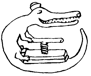
\includegraphics[width=\linewidth]{lutembi}
%   \caption[Crocodile]{Crocodile from the CoP website}
% \label{img1}
%   \end{minipage}
%   \hspace{.05\linewidth}
%   \begin{minipage}{.275\linewidth}
%     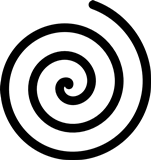
\includegraphics[width=\linewidth]{spiral01}
%   \caption[Gidouille]{\raggedleft The Grand Gidouille}
% \label{img2}
%   \end{minipage}
%   \hspace{.05\linewidth}
%   \begin{minipage}{.275\linewidth}
%     
\includegraphics[width=\linewidth]{greencandle}
%   \caption[Green Candle]{The green candle}
% \label{img3}
%   \end{minipage}
% \end{figure}


\subsection{Antimony}
\label{s:antinomy}

The antimony is the mutually incompatible. It appears everywhere in Jarry's writings. It represents the duality of things, the echo or symmetry, the good and the evil at the same time. Examples are the plus-minus, the faust-troll, the haldern-ablou, the yes-but, the ha-ha and the paradox.

The `Ha Ha', the only words Bosse-da-Nage ever utters in Faustroll, ``is the idea of duality, of echo, of distance, of symmetry, of greatness and duration, of the two principles of good and evil.'' \autocite{Hugill2012a} Referring to the yes-but statement, Hugill says ``this may be taken as a standard pataphysical response to any proposition (including this one).'' And most obviously the antimony can be seen in all the contradictions that pataphysics is so fond of.


\subsection{Anomaly}
\label{s:anomaly}

The anomaly is the exception. And exceptions are important in pataphysics. But then again everything is equal, so in a pataphysical world no exceptions would exist at all, or rather, everything would be equally exceptional. The anomaly disrupts and surprises. Hugill mentioned a great example of a collection of anomalies: the sourcebook project by William Corliss, who collects scientific papers that are anomalous. Bök says it is ``the repressed part of a rule which ensure that the rule does not work'' \citeyear[p.38]{Boek2002}.

\todo{mention Bergson and Hegel here?}


\subsection{Syzygy}
\label{s:syzygy}

The syzygy surprises and confuses. It originally comes from astronomy and denotes the alignment of three celestial bodies in a straight line. In a pataphysical context it is the pun, which Jarry called ``the syzygy of words'' \citeyear{Jarry1996}. It usually describes a conjunction of things, something unexpected and surprising. Next to being intentionally funny, puns demonstrate a clever use (or abuse) of grammar, syntax, pronunciation and/or semantics, often taken to a quite scientific level, such that without understanding of what is said and what is the intended meaning, the humour of the pun might be lost. Serendipity is a simple chance encounter but the syzygy has a more scientific purpose. Bök mentions Jarry saying that ``the fall of a body towards a centre is the same as the ascension of a vacuum towards a periphery'' \citeyear[p.42]{Boek2002}.


\subsection{Clinamen}
\label{s:clinamen}

The clinamen is the unpredictable swerve that Bök calls ``the smallest possible aberration that can make the greatest possible difference'' \citeyear[p.43]{Boek2002}. He links it to Lucretius idea of an atom swerving in its streamlined flow to create matter and to Epicurus' parenklisis. But he also points out similarities to ideas like the Situationists' `détournement', the reuse of pre-existing aesthetic elements and Hugill links it to the Dadaists' ready-mades and Oulipo's verbal games \citeyear{Hugill2012a}. An obvious example is Jarry's \emph{merdre}, a swerve of the French word for shit (merde).


\subsection{Absolute}
\label{s:absolute}

The absolute is a reference to a transcended reality. Jarry talks about `ethernity' in Faustroll \citeyear[p.104]{Jarry1996}.


\section{Unconscious}

\subsection{Oulipo}
\label{s:patalipo}

\begin{quotation}
  Potential literature is ``the search for new forms and structures that may be used by writers in any way they see fit.'' \sourceatright{Raymond Queneau in \autocite[p.2]{Motte2007}}
\end{quotation}

% \begin{quotation}
%   The Oulipo's goal is to discover new structures and to furnish for each structure a small number of examples. \sourceatright{François Le Lionnais in \autocite[p.3]{Motte2007}}
% \end{quotation}

\begin{quotation}
  What is the objective of our work? To propose new ``structures'' to writers, mathematical in nature, or to invent new artificial or mechanical procedures that will contribute to literary activity: props for inspiration as it were, or rather, in a way, aids for creativity. \sourceatright{Raymond Queneau in \autocite[p.51]{Motte2007}}
\end{quotation}

The \ac{oulipo} was already introduced in chapter~\ref{s:oulipo}\marginnote{§~\ref{s:oulipo}} as one of my main inspirations and influences on this research.

The \ac{OULIPO} is an originally literary movement from the 1960's, originating in France as a subcommittee of the ``Coll\`{e}ge de \'Pataphysique''. It has since spread to other disciplines. The generic term for Oulipian groups is OUXPO (``Ouvroir d'X Potentielle''), where the X can be replaced with whatever particular subject area you like (typically in french): fine art---OUPEINPO, music---OUMUPO, etc. It has roots in pataphysics although it eventually separated and became a standalone group. Their main philosophy perhaps is to use constraints in order to enhance creative output. Some examples of techniques, taken from \autocite{Mathews2005}, invented and used by them are shown below.

Techniques such as the famous `N+7', `melting snowball' and `Mathew\'s Algorithm' (see chapter~\ref{s:oulipo} and figure~\ref{fig:poems}\marginnote{\faicon{object-group}~\ref{fig:poems}}) are typical examples of oulipian methods. They have endless applications in as many different disciplines. Motte collated a useful overview of the different Oulipian operations \citeyear[p.44--45]{Motte2007}, shown here in table~\ref{tab:oulipo1} and table~\ref{tab:oulipo2}\marginnote{\faicon{table}~\ref{tab:oulipo1} + \ref{tab:oulipo2}}.

\begin{table}[!htbp]
\caption[Oulipo Operations I]{Oulipo---Elementary Linguistic and Literary Operations---Part I}
\label{tab:oulipo1}
{\footnotesize
\begin{tabu}{X[l,0.7]X[l]X[l]X[l]}
  \toprule
  & \textbf{Letter}
  & \textbf{Phoneme}
  & \textbf{Syllable}
  \\ \midrule
  \textbf{Displacement} 
  & anagram, palindrome, pig Latin, metathesis 
  & phonetic palindrome, spoonerism, Rrose S{\'e}lavy (Desnos), glossary (Leiris)
  & syllabic palindrome, spoonerism
  \\
  \textbf{Substitution} 
  & paragram (printer's error), cryptography
  & {\`a}-peu-pr{\`e}s, alphabetical drama
  &
  \\
  \textbf{Addition} 
  & prosthesis, epenthesis, paragoge
  & stuttering
  & Javanese stuttering, germination, echolalia 
  \\
  \textbf{Subtraction} 
  & abbreviation, aphaeresis, syncope, elision, lipogram, belle absente, constraint of the prisoner
  & lipophoneme
  & haplography, liposyllable (Precious [con]straint), shortening
  \\
  \textbf{Multiplication (repetition)} 
  & tautogram
  & alliteration, rhyme, homoeuteleuton
  & stuttering, alliteration, rhyme
  \\
  \textbf{Division} 
  &
  &
  & diaeresis
  \\
  \textbf{Deduction} 
  & acrostic, acronym, signet, chronogram
  & 
  & acronym
  \\
  \textbf{Contraction}
  & crasis
  &
  & 
  \\
  \bottomrule
\end{tabu}
}
\end{table}

\begin{table}[!htbp]
\caption[Oulipo Operations II]{Oulipo---Elementary Linguistic and Literary Operations---Part II}
\label{tab:oulipo2}
{\footnotesize
\begin{tabu}{X[l,0.85]X[l,1.2]X[l,1.2]X[l,0.7]X[l,0.7]}
  \toprule
  & \textbf{Word}
  & \textbf{Syntagm}
  & \textbf{Sentence}
  & \textbf{Paragraph}
  \\ \midrule
  \textbf{Displacement} 
  & Mathews's Algorithm, permutations (Lescure), word palindrome, inversion
  & reversion, inversion, anastrophe
  & Mathews's Algorithm
  & Mathews's Algorithm
  \\
  \textbf{Substitution} 
  & metonymy, S + 7, homosyntaxism, L.S.D., translation, antonymic translation
  & perverbs (Mathews), proverbs, aphorism, homophony, untraceable locutions
  & homophony, holorhyme
  &
  \\
  \textbf{Addition} 
  & redundance, pleonasm
  & interpolation, encasement
  & tireur {\`a} la ligne, larding
  & tireur {\`a} la ligne
  \\
  \textbf{Subtraction} 
  & liponym, La Rien que la Toute la (Le Lionnais)
  & ellipsis, brachylogia, zeugma
  & coupeur {\`a} la ligne
  & censure
  \\
  \textbf{Multiplication (repetition)} 
  & epanalepsis, pleonasm, anaphora, defective rhyme
  & reduplication
  & leitmotif, refrain
  &
  \\
  \textbf{Division} 
  & de-portmanteau word, etymology, tmesis 
  & Roussellian procedure (phonic dislocation), hendiadys
  & dislocation
  &
  \\
  \textbf{Deduction} 
  & haikuization
  & proverbs on rhymes, edges of poem
  & citation, tireur {\`a} la ligne, collage
  & plagiarism, anthology
  \\
  \textbf{Contraction}
  & portmanteau word
  & syntagmatic amalgam (Doukipudonktan)
  &
  & r{\'e}sum{\'e}
  \\
  \bottomrule
\end{tabu}
}
\end{table}

The Oulipian aesthetic is a paradox--- formal constraints afford creative liberty, Motte says \citeyear[p.18]{Motte2007}. He also explained that ``Erecting the aesthetic of formal constraint, then, the Oulipo simultaneously devalues inspiration'' \autocite[p.10]{Motte2007}. François Le Lionnais defined the following three levels in the hierarchy of constraints \autocite[p.11]{Motte2007}. (1) Minimal: constraints on the language in which the text is written, (2) Intermediate: constraints on genre and certain literary norms, and (3) Maximum: consciously preelaborated and voluntarily imposed systems of artifice. The use of constraints combats the aleatory or random.

\begin{quotation}
  The Oulipo is anti-chance. \sourceatright{Claude Berge in \autocite[p.17]{Motte2007}}
\end{quotation}


\subsection{Borges}

The influence of Jose Luis Borges was already briefly discussed in chapter~\ref{s:borges}\marginnote{§~\ref{s:borges}}. Hugill sees him as an unconscious pataphysician \citeyear{Hugill2012a}.

Borges' text \textit{The analytical language of John Wilkins} \citeyear{Borges2000} contains a brilliant example of pataphysical thinking and coincidentally a good example of the kinds of search results my search tool should hopefully produce.

Referring to a certain Chinese dictionary entitled ``The Celestial Emporium of Benevolent Knowledge'' animals can be divided into:

\begin{enumerate}
  \item	those belonging to the Emperor
  \item	those that are embalmed
  \item	those that are tame
  \item	pigs
  \item	sirens
  \item	imaginary animals
  \item	wild dogs
  \item	those included in this classification
  \item	those that are crazy-acting
  \item	those that are uncountable
  \item	those painted with the finest brush made of camel hair
  \item	miscellaneous
  \item	those which have just broken a vase
  \item	those which, from a distance, look like flies
\end{enumerate}

This kind of categorisation has also been discussed by Foucault in his book \textit{The Order of Things} \citeyear{Foucault1966}.

\spirals

Other concepts that are pataphysical or can be linked to it in a sense are alchemy and quantum mechanics. Alchemy because of its laws or equivalence and the union of opposites \autocite{Hugill2012a} and quantum mechanics because of principles of uncertainty, indeterminacy and the idea of the multiverse of course.

\begin{quotation}
  Because string theory is speculation based on ideas that are themselves speculative (i.e., theories of general relativity and quantum mechanics), string theory is not in fact physics, but 'pataphysics.

  Likewise, string theory and quantum calculations are, increasingly, not descriptive of an actual reality, but are simply mathematical pataphors. \sourceatright{\autocite{pataphysics2007}}
\end{quotation}

\stopcontents[chapters]

% % !TEX root = ../main.tex

\chapter{Creativity}
\label{ch:creativity}

\startcontents[chapters]

\vfill

\begin{alltt}\sffamily
From high Olympus prone her flight she bends,
rare courage and grandeur of conception,
congratulating herself apparently on the cleverness,
appeared distorted to my vision.

Had he had any bad design,
having uttered these words the vision left me,
if any thought by flight to escape,
taking his flight towards warmer and sunnier regions.

Inspire à mon oncle cette vision décourageante de l'avenir,
être et l'invention du jeu de ce,
besoin de satisfaire l'imagination d'objets rares ou grandioses.

Some may call vision,
a man of invaluable ability,
mobiles parois de L'imagination.
\end{alltt}

\newpage
\minicontents
\spirals

Creativity does not have a universally accepted definition. Creativity is a human quality and definitions don't necessarily lend themselves to be applied to computers as well. There are aspects that come up often, like novelty and value, but some that rarely pop up, like relevance and variety. Creativity can be studied at various `levels' (neurological, cognitive, and holistic/systemic), from different `perspectives' (subjective and objective) and `characteristics' (combinational, exploratory and transformative). Creativity should be seen as a continuum, there is no clear cut-off point or Boolean answer to say precisely when a person or piece of software has become creative or not.

Linda Candy identified 3 approaches for studying creativity \autocite*{Candy2012}:

\begin{description}
  \item [Research Design] Experimental, psychometric, observational, \ldots
  \item [Research Focus] Human attributes, cognitive processes or creative outcomes.
  \item [Research Evidence] Real-time observation, historical data, artificial (laboratory) or natural (real world settings).
\end{description}

Richard Mayer identified five big questions of human creativity research and different approaches with their own methodologies and goals \autocite*{Mayer1999}:

\label{s:Mayer5questions}
\begin{enumerate}
  \item Is creativity a property of people, products, or processes?
  \item Is creativity a personal or social phenomenon?
  \item Is creativity common or rare?
  \item Is creativity domain-general or domain-specific?
  \item Is creativity quantitative or qualitative?
\end{enumerate}

\begin{description}[leftmargin=3.5cm]
  \item [Psychometric] (creativity as a mental trait): quantitative measurement, controlled environments, ability based analysis
  \item [Psychological] (creativity as cognitive processing): controlled environments, quantitative measurements, cognitive task analysis
  \item [Biographical] (creativity as a life story): authentic environments, qualitative descriptions, quantitative measurements
  \item [Biological] (creativity as a physiological trait): physiological measures
  \item [Computational] (creativity as a mental computation): formal modelling
  \item [Contextual] (creativity as a context-based activity): social, cultural and evolutionary context
\end{description}

Mayer identified the challenge of developing a ``clearer definition of creativity'' and ``a combination of research methodologies that will move the field from speculation to specification'' \autocite*{Mayer1999}.

This chapter introduces relevant models of human and computer creativity and describes the disciplines of computational creativity and creative computing.


\section{In Humans}
\label{s:humancreativity}

Creativity is usually defined as \emph{the ability to use original ideas to create something new and surprising of value}. We generally speak of creative `ideas' rather than products, since creative products merely provide evidence of a creative process that has already taken place.

\begin{quotation}
  Creativity is the interaction among aptitude, process, and environment by which an individual or group produces a perceptible product that is both novel and useful as defined within a social context \sourceatright{\autocite[Plucker et al, as cited in][]{Jordanous2012}}
\end{quotation}


\subsection{Four Stages}
\label{s:4stages}

Henri Poincar{\'e} and Graham Wallas have defined a popular model of the creative process (it was suggested by Poincar{\'e} \autocite*{Poincare2001} and formulated by Wallas \autocite*{Wallas1926}). This model has been picked up by many researchers since, including \autocite{Boden2003, Koestler1964, Partridge1994}.

\begin{enumerate}
  \item Preparation – focusing the mind on the problem
  \item Incubation – unconscious internalising
  \item Illumination – eureka moment from unconsciousness to consciousness
  \item Verification – conscious evaluation of the idea and elaboration…
\end{enumerate}

Weisberg, however, criticises the stages of incubation and illumination \autocite[as cited in][]{Partridge1994}, saying that the creative process is really just simple problem solving, and that incubation is what he calls `creative worrying'. Problem solving was defined in similar steps by George P{\'o}lya \autocite*{Polya1957}.

\begin{quotation}
  First, we have to \textbf{understand} the problem; we have to see clearly what is required. Second, we have to see how the various items are connected, how the unknown is linked to the data, in order to obtain the idea of the solution, to make a \textbf{plan}. Third, we \textbf{carry out} our plan. Fourth, we \textbf{look back} at the completed solution, we review and discuss it. \sourceatright{\autocite[][his emphasis]{Polya1957}}
\end{quotation}


\subsection{Four P's}
\label{s:fourp}

Mel Rhodes identified four common themes of creativity, which he termed ``the four P\rq s of creativity'' \autocite*{Rhodes1961}:

\begin{description}[leftmargin=2.5cm]
  \item [Persons] personality, intellect, temperament, physique, traits, habits, attitudes, self-concept, value systems, defence mechanisms and behaviour.
  \item [Process] motivation, perception, learning, thinking and communication.
  \item [Press] relationship between human beings and their environment
  \item [Products] a thought which has been communicated to other people in the form of words, paint, clay, metal, stone, fabric, or other material.
\end{description}

Rhodes highlighted the importance of a holistic view on creativity through these four areas of study, which he hoped would become the basis of a unified theory of creativity.

In a similar fashion, Ross Mooney identified four aspects of creativity \autocite[as cited in][]{Sternberg1999}.

\begin{enumerate}
  \item The creative environment
  \item The creative person
  \item The creative process
  \item The creative product
\end{enumerate}


\subsection{Four C's}
\label{s:fourc}

James Kaufman and Ronald Beghetto developed a model of creativity called the ``four C model'' \autocite*{Kaufman2009}. Figure~\ref{fig:4C}\sidepar{\faicon{object-group}~\ref{fig:4C}} shows the relationship between the so called 4 C's.

\begin{figure}[!htbp]
  \centering
  \begin{tikzpicture}[node distance = 2cm and 7cm]
    \node [box] (minic) {mini-c};
    \node [box, below = of minic] (littlec) {little-c};
    \node [box, right = of minic] (proc) {Pro-c};
    \node [box, right = of littlec] (bigc) {Big-C};
    \node [above = 1cm of proc] (stasis) {Stasis};
    \node [below = 1cm of bigc] (legend) {Legend};
    \node [below = 1cm of littlec] (reflect) {Reflection};
    \draw [sa] (minic) -- node [left] {Tinkering} (littlec);
    \draw [sa] (minic) -- node [above] {Formal Apprenticeship} (proc);
    \draw [sa] (littlec) -- node [below = 10pt, text width = 2cm] {Informal Apprenticeship} (proc);
    \draw [sa] (littlec) -- (reflect);
    \draw [sa] (proc) -- (stasis);
    \draw [sa] (proc) -- (bigc);
    \draw [sa] (bigc) -- (legend);
    \draw [sa] (proc) -| +(1.4,0) |- node[near start, right] {Greatness} (bigc);
  \end{tikzpicture}
\caption[The 4 C model]{The 4 C model}
\label{fig:4C}
\end{figure}

\begin{description}[leftmargin=1.9cm]
  \item [Big-C] \textit{Eminent Accomplishments}. Consists of clear-cut, eminent creative contributions. It often requires a degree of time. Indeed, most theoretical conceptions of Big-C nearly require a posthumous evaluation.
  \item [Pro-c] \textit{Professional Expertise}. Represents the developmental and effortful progression beyond little-c. The concept of Pro-c is consistent with the expertise acquisition approach of creativity.
  \item [Little-c] \textit{Everyday Innovation}. More focused on everyday activities, such as those creative actions in which the non-expert may participate each day.
  \item [Mini-c] \textit{Transformative Learning}. Encompasses the creativity inherent in the learning process. ``Mini-c is defined as the novel and personally meaningful interpretation of experiences, actions, and events.'' \autocite{Beghetto2007} Central to the definition of mini-c creativity is the dynamic, interpretive process of constructing personal knowledge and understanding within a particular socio-cultural context. Moreover, mini-c stresses that mental constructions that have not (yet) been expressed in a tangible way can still be considered highly creative. Mini-c highlights the intrapersonal, and more process focused aspects of creativity.
  \item [All 4 C's] Openness to new experiences, active observation, and willingness to be surprised and explore the unknown.
\end{description}


\subsection{Four Types}
\label{s:personality}

Sternberg and Kaufman identified a set of personality traits that are associated with creative people in their \textit{Handbook of Creativity} \autocite*{Sternberg1999}. These are: independence of judgement, self-confidence, and attraction to complexity, aesthetic orientation, and tolerance for ambiguity, openness to experience, psychoticism, risk taking, androgyny, perfectionism, persistence, resilience, and self-efficacy. It is easy to find common characteristics among creative people but that doesn't mean that these automatically make a person or a product creative.

Timothy Leary took this idea of common characteristics a bit further and suggested there are four types of creative personalities \autocite*{Leary1964}. From his ideas we can draw the conclusion that a creative person needs to be able to make novel combinations from novel ideas.

\begin{description}
  \item [Reproductive Blocked] no novel combinations, no direct experience
  \item [Reproductive Creator] no direct experience, but crafty skill in producing new combinations of old symbols
  \item [Creative Creator] new experience presented in novel performances
  \item [Creative Blocked] new direct experience expressed in conventional modes
\end{description}

Tables~\ref{tab:Leary1} and~\ref{tab:Leary2} in appendix~\ref{s:leary}\sidepar{§~\ref{s:leary}} are in Leary's words and show the detailed description of these personality types.


\subsection{Three Domains}
\label{s:koestler}

Arthur Koestler published his study on creativity entitled \textit{The Act of Creation} \autocite*{Koestler1964}. His main contribution to the field is probably the concept of `bisociation', a term he coined for the idea of two ``self-consistent but habitually incompatible frames of reference'' intersecting to give rise to new creative ideas \autocite*{Koestler1964}. It is interesting however to look at some of his other views on creativity as well.

He splits creativity into three domains---a triptych---without sharp boundaries: humour, discovery and art (see table~\ref{tab:KHDA}\sidepar{\faicon{table}~\ref{tab:KHDA}}). All creative acts traverse the three domains of this triptych from left to right, that is, the emotional climate of the creator changes ``from an absurd through an abstract to a tragic or lyric view of existence'' during the process \autocite*{Koestler1964}. Central to all three domains is the ``discovery of hidden similarities'', or bisociation. Koestler differentiates between associative thinking and bisociative thinking. He links those broadly to habit and originality, respectively. More specifically, associative thinking is conscious, logical, habitual, rigid, repetitive and conservative and bisociative thinking is unconscious, intuitive, original, flexible, novel and destructive/constructive.

% \begin{table}[!htbp]
% \caption[Associative vs Bisociative]{Koestler: Associative vs Bisociative}
% \label{KAB}
%   \centering
%   \begin{tabu}{cc}
%   \toprule
%   \textbf{Associative} & \textbf{Bisociative}     \\
%   \midrule
%   Conscious            & Unconscious              \\
%   Logic                & Intuition                \\
%   Habit                & Originality              \\
%   Rigid                & Flexible                 \\
%   Repetitive           & Novel                    \\
%   Conservative         & Destructive/Constructive \\
%   \bottomrule
%   \end{tabu}
% \end{table}

\begin{table}[!htbp]
\caption[Koestler's creative triptych]{Koestler's creative triptych}
\label{tab:KHDA}
  \centering
  \begin{tabu}{ccccc}
  \toprule
  \textbf{Humour} & $\to$ & \textbf{Discovery} & $\to$ & \textbf{Art} \\
  \midrule
  Laugh           && Understand         && Marvel       \\
  Riddle          && Problem            && Allusion     \\
  Debunking       && Discovering        && Revealing    \\
  Coincidence     && Trigger            && Fate         \\
  Aggressive      && Neutral            && Sympathetic  \\
  \bottomrule
  \end{tabu}
\end{table}


\subsection{Three Processes}
\label{s:boden}

Margaret Boden is often cited in the fields of \acf{CC} and computational creativity. Her main interest is in how the human mind works and how computer models of the mind and specific thinking processes can help us understand both better. She has provided two important contributions to the field. The first is her description of three distinct forms of creativity describes in this section and the second is her important distinction between two senses of creativity as described in section~\ref{s:pandh}\sidepar{§~\ref{s:pandh}} \autocite{Boden2003}.

\begin{quotation}
  [Creativity is] the ability to come up with ideas or artefacts that are \textbf{new, surprising and valuable}. \sourceatright{\autocite[][her emphasis]{Boden2003}}
\end{quotation}

She identified three distinct forms or cognitive processes of how creativity can happen. These are combinational, exploratory and transformational creativity, which can happen at the same time \autocite{Boden2003}.

\begin{description}
  \item [Combinational creativity] making unfamiliar combinations of familiar ideas; juxtaposition of dissimilar; bisociation; deconceptualisation
  \item [Exploratory creativity] exploration of conceptual spaces; noticing new things in old spaces
  \item [Transformative creativity] transformation of space; making new thoughts possible by altering the rules of old conceptual space
\end{description}

Central to these three forms is the idea of a `conceptual space'. For any idea, its conceptual space describes the characteristics and constraints that define it in its most fundamental way. The conceptual space of a tea cup would contain information like: it is a container that can hold a hot fluid, it should hold about a half a pint of fluid and it might or might not be built in such a way as to not burn the hand that carries it. The specific colour of the cup or what material it is made of for example are not contained in its conceptual space.

Combinational creativity is the most common form of the three and is concerned with the unusual juxtaposition of common ideas. This aspect is highlighted in her definition of creativity, which requires novelty and surprise. The main idea is that any particular combination of ideas has to be unusual, causing surprise, but not (necessarily) the individual ideas themselves. She safeguards against purely random combination by including the usefulness of the result as a requirement in the definition. Exploratory creativity requires a person (or computer program) to fully explore the conceptual space of an idea and find unusual or interesting aspects of it. This form of creativity is about pushing an idea to its limits. Transformational creativity takes this exploration one step further. Once the limits of an idea have been identified, they can be transformed. This means that we can step out of the normal conceptual space of an idea, create a new one, alter or ignore the given constraints, add new ones, etc.

Boden argues that creative ideas are surprising because they go against expectations \autocite*{Boden2003}. She also believes that constraints support creativity and are even essential for it to happen, which echos the \ac{OULIPO} philosophy mentioned in chapter~\ref{s:patalipo}\sidepar{§~\ref{s:patalipo}}.

\begin{quotation}
  Constraints map out a territory of structural possibilities which can then be explored, and perhaps transformed to give another one. \sourceatright{\autocite{Boden2003}}
\end{quotation}

Bipin Indurkhya argues that there are two main cognitive mechanisms of creativity: namely juxtaposition of dissimilar and deconceptualisation. He says that we are constrained by associations of our concept networks that we inherit and learn in our lifetime, but that computers do not have those conceptual associations and have therefore an advantage when it comes to creative thinking \autocite*{Indurkhya1997}.


\subsection{Two Levels}
\label{s:pandh}

The three processes of creativity mentioned in the previous section\sidepar{§~\ref{s:boden}} can be then interpreted on two levels \autocite{Boden2003}. Any idea should be viewed and evaluated at the appropriate level. Consider the following scenario. A child and a professional architect both build a corbeled arch out of material available to them. Who is being creative here? The level of expertise is clearly different between the two. The child has no experience and is experimenting with the possibilities and limitations of the building blocks (exploring their conceptual space) while the architect has studied the technique for years and is simply applying knowledge he has learned from others (familiar use of a familiar idea). Clearly the child is being more creative in this example. Boden proposed to view and judge the creativity of these two persons separately by differentiating between two levels of creativity, a personal one and a historical one. 

`Psychological creativity' (P-creativity) is a personal kind of creativity that is novel in respect to an individual and `historical creativity' (H-creativity) is fundamentally novel in respect to the whole of human history \autocite{Boden2003}. 

The child in the earlier scenario was P-creative but the architect was neither, he was simply applying his trained skills.

\begin{quotation}
	P–creativity involves coming up with a surprising, valuable idea that's new to the person who comes up with it. It doesn't matter how many people have had that idea before. But if a new idea is H–creative, that means that (so far as we know) no one else has had it before: it has arisen for the first time in human history. \sourceatright{\autocite{Boden2003}}
\end{quotation}


\section{In Computers}
\label{s:compcreativity}

This section introduces some models that try to implement creative thinking models in computers. It is really just a survey of different concepts and views and does not immediately apply to my specific research on creative search tools.

Partridge and Rowe conducted a survey of computational models of creativity in their book \textit{Computers and Creativity} \autocite*{Partridge1994}. They mention the computer as an unbiased\footnote{I will later argue that this is not possible, since a computer cannot be judged without taking the programmer into account. See chapter~\ref{s:programmer} for more details.} medium for executing creative programs. Some of the computational methodologies they discussed are as follows, many taken from classical \ac{AI} research. These are: generative grammars, discovery programs, rule based systems, meta-rules (which reason about and create new rules), analogical mechanisms, flexible representations, classifier systems, decentralised systems, connectionist systems, neural networks, and emergent memory models. Classifier systems for example, consist of a set of rules and a message list as shown below.

\begin{enumerate}
  \item Place input messages on current message list.
  \item Find all rules that can match messages.
  \item Each such rule generates a message for the new message list.
  \item Replace current message list with the new one.
  \item Process new list for any system output.
  \item Return to step 1.
\end{enumerate}

These can easily be combined with genetic algorithms to enable the system to learn an appropriate classifier set. This is called emergent behavior. Another approach is connectionism also known as neural networks. Partridge and Rowe then go on to describe their emergent-memory model. They are applying the ideas of Poincar{\'e} and Wallas \autocite{Poincare2001,Wallas1926} and are heavily influence by Minsky's theory of K-lines \autocite*{Minsky1980,Minsky1988}. They define the following characteristics for creative programs:

\begin{itemize}
  \item flexible knowledge representation scheme
  \item representational imprecision
  \item multiple representations
  \item self-assessment
  \item full elaboration
\end{itemize}

\spirals

Gelernter introduced a theory of how the human mind works called the `spectrum model' \autocite*{Gelernter1994}. It is based on the idea of mental focus and relates well to creativity. According to him we have a thought spectrum. The higher the mental focus, the more awake we are, the more adult we are and modern, logical and rational, convergent, abstract and detailed. The less focused we are the younger or ancient or dreaming we are. Low focus thoughts are metaphoric, hallucinations, divergent, creative, inspirations, concrete, ambient and emotional. Emotions glue low focus thoughts together.

He gives a good example of his own computer program that is being trained by a set of simple pairs (or memories) in the form \textbf{mood: happy} for example. These sets of pairs form the experience of the system, the memory that the system can access. It's fetching all memory pairs that match a certain probe, then generalizes them and picks out a feature that is common to all and then uses that to probe further if necessary.

He models his spectrum concept in a way that if we want the system to operate at low focus, more memory pairs would be fetched and more generalised features are deducted and so on. He describes his FGP program (Fetch Generalise Project) as follows \autocite{Gelernter1994}.

\begin{enumerate}
  \item Fetch memory pairs in response to a probe (question).
  \item Sandwich them together and peer through the bundle at once.
  \item Notice the common features that emerge strongly (generalise).
  \item Pick out interesting emergent details and probe further if necessary.
\end{enumerate}

With low focus the system would not generalise as much and just pick out a particular memory, etc. The computer system Gelernter has built seems very limited. His memory pairs cannot describe everything. For example they can describe states but not actions.

This idea of accessing thoughts/memories is very closely related to searching. Searching an index in a search engine is similar to remembering, trying to find all memories related to the current thought for example.

\spirals

Minsky introduced the concepts of K-lines in his \textit{Society of Mind} \autocite*{Minsky1980, Minsky1988}. It is basically a theory of memory. He claims that the ``function of a memory is to recreate a state of mind''. His theory of k-lines is as follows.

\begin{quotation}
  When you get an idea, or solve a problem, or have a memorable experience, you create what we shall call a K-line. This K-line gets connected to those mental agencies that were actively involved in the memorable mental event. When that K-line is later activated, it reactivates some of those mental agencies, creating a partial mental state resembling the original. \sourceatright{\autocite{Minsky1980, Minsky1988}}
\end{quotation}

This theory works quite well with Gelernter's idea of memory. K-lines in this sense are nothing other than Gelernter's memory pairs.

Minsky and his student Push Singh have formalised the idea of a panalogy\footnote{The concept of the panalogy was originally discussed in the initial proposal for this research project. See section~\ref{s:surfer}}. The idea is that an idea can and should be conceptualised in many different ways. This could be seen as a fall-back mechanism for computational models, if one approach didn't return the desired/expected results.

\spirals

Elton explains the concept of `artificial creativity' which can be seen as a sub-area of \ac{AI}. \ac{AI} research isn't `human' enough, he argues, it needs to include less abstract ideas like emotions, morals, aesthetic sensibility and creativity. He goes on to explain in detail how production, evaluation and etiology play a role in everything \autocite{Elton1995}.

Opposed to the traditional approach of \ac{AI} to study some aspect of the human brain in a specific domain only, he argues that in order to understand creativity we need to look at more than that. Creativity arises from a process that is not isolated. The etiology (its history) is essential for something to be classed as creative. Generation (of artefacts or ideas) cannot count as creative if it doesn't undergo evaluation in the process. In order to evaluate we need a sound knowledge of the relevant domain. 

\begin{quotation}
  We want creative evaluation to be influenced by a longstanding history of interaction with entities (of whatever kind) in the world. \sourceatright{\autocite{Elton1995}}
\end{quotation}
  
Computer systems can be seen in two perspectives: plastic and implastic (resettable). Elton argues that ``all systems can be seen from the implastic perspective since ultimately all systems are built out of physical components that are (statically) well behaved, but for certain explanatory purposes some are best understood plastically'' \autocite*{Elton1995}. Connectionist networks are an example of a plastic system. The brain is a plastic system too.

% \begin{shaded}
%   Summary\\
%   •	Boden: Combinational, exploratory and transformative \autocite{Boden2003, Wiggins2006} (process)\\
%   •	Boden: new, surprising, valuable \autocite{Boden2003} (product)\\
%   •	Colton: Skill + appreciation + imagination = creativity (or the appearance of) \autocite{Colton2008a} (product+process)\\
%   •	Wiggins: relevance + acceptability + quality \autocite{Wiggins2006} (product)\\
%   •	Ritchie: typicality + quality \autocite{Ritchie2001, Ritchie2007} (product)\\
%   •	Pease: novelty + value \autocite{Pease2001} (product+process)\\
%   •	Ventura: efficiency + variety \autocite{Ventura2008} (product+process)\\
%   •	Jordanous: value (related concepts: usefulness, appropriateness, relevance) + novelty (related concepts: originality, newness) \autocite{Jordanous2012}
% \end{shaded}


\section{In Academia}

Two transdisciplinary fields of study have emerged from the variety of disciplines concerned. These are computational creativity and creative computing. The former\sidepar{§~\ref{s:compcrea}} lies at the cross section of \ac{AI} and cognitive science and is about achieving creativity through computation and the latter\sidepar{§~\ref{s:creacomp}} is mostly distinguished by its involvement in art and is about doing computations in a creative way. Creative computing focuses on the process of creativity and `tacit knowledge' rather than just the outcome as is more often the case in computational creativity. There is also an area called speculative computing\sidepar{§~\ref{s:speccomp}} discussed later on.

The concept of creative computing has existed for some time but is only just starting to evolve into a recognised mainstream discipline within computer science. As of 2016, there is a journal \autocite{IJoCCnd}, conference \autocite{ISCC2016} and several undergraduate courses dedicated to creative computing\footnote{Courses (in the UK) are offered by Bath Spa University, University of the Creative Arts, Edinburgh Napier University, Glyndwrd University, Goldsmiths University of London, Queen Mary University of London, and University of West London (according to UCAS 2016)}. Computational creativity, on the other hand, has emerged as a field within \ac{AI} research and overlaps with creative computing ideas to some extent. There's also a conference \autocite{ICCC2017}, which has been going for several years.

Perhaps a good example of creative computing is the International Obfuscated C Code Contest \autocite{Broukhis}. The competition revolves around writing compilable/runnable code, while visually appearing as obfuscated as possible. They value unusuality, obscurity and creativity but expect contestants to follow the strict rules and constraints of the C programming language. Obfuscation in itself isn't necessarily the hallmark of creative computing but it is one possible use-case. See the example competition entry shown on page~\pageref{code:goren}\sidepar{\faicon{code}~\ref{code:goren}}.

Examples of computational creativity are Simon Colton's \textit{Painting Fool} \autocite*{Coltonnd} or Harold Cohen's \textit{AARON} \autocite{kurzweilcyberartnd}; both are computer programs that paint pictures. Kurzweil's \textit{Cybernetic Poet} \autocite{kurzweilcyberart2001} is a classic example of a program that produces poetry.

\spirals

But how may we apply the insights into creativity described in chapter~\ref{s:humancreativity}\sidepar{§~\ref{s:humancreativity}} to computing? One approach is described by Simon Colton \autocite*{Colton2008}, who suggests we should adopt human skill, appreciation and imagination.

\begin{quotation}
  Without skill, they would never produce anything. Without appreciation, they would produce things which looked awful. Without imagination, everything they produced would look the same. \sourceatright{\autocite{Colton2008}}
\end{quotation}

He thinks that evaluating the worth of an idea or product is the biggest challenge facing computational creativity. Whereas in conventional problem solving success is defined as finding a solution, in a creative context more aesthetic considerations have to be taken into account. 


\subsection{Computational Creativity}
\label{s:compcrea}

Computational creativity is a relatively new discipline and as such not well defined. Simon Colton, the creator of the \textit{Painting Fool}, describes it as the discipline of generating artefacts of real value to someone \autocite*{Colton2008}. This is in contrast to classic \ac{AI} problem solving.

One could say that computational creativity is the attempt at giving computers the skills, appreciation and imagination needed to produce creative artefacts. Whether or not this makes the computer creative, or the programmer, is another question that I will address in chapter~\ref{ch:interpretation}\sidepar{§~\ref{ch:interpretation}}.

Computational creativity has emerged from within \ac{AI} research. Simon Colton and Geraint Wiggins argue \ac{AI} falls within a problem solving paradigm: ``an intelligent task, that we desire to automate, is formulated as a particular type of problem to be solved'' \autocite*{Colton2012}, whereas ``in Computational Creativity research, we prefer to work within an artefact generation paradigm, where the automation of an intelligent task is seen as an opportunity to produce something of cultural value'' \autocite*{Colton2012}. Hugill and Yang on the other hand argue its role within computer science falls under the scientific paradigm \autocite*{Hugill2013c}, \autocite[see also][]{Eden2007}, as opposed to \acf{CC} in the technocratic paradigm.

The \acf{ACC} promotes the advancement of computational creativity which they define as follows.

\begin{quotation}
  Computational Creativity is the art, science, philosophy and engineering of computational systems which, by taking on particular responsibilities, exhibit behaviours that unbiased observers would deem to be creative. \sourceatright{\autocite{iccc2014}}
\end{quotation}

Computational creativity is multidisciplinary, bringing together researchers from \ac{AI}, cognitive psychology, philosophy, and the arts.  Its main goal is to model, simulate or replicate human creativity using a computer and it has the following three aims:

\begin{itemize}
  \item to construct a program or computer capable of human-level creativity
  \item to better understand human creativity and to formulate an algorithmic perspective on creative behavior in humans
  \item to design programs that can enhance human creativity without necessarily being creative themselves
\end{itemize}

The \acf{ACC} manages the annual \ac{ICCC}, whose recent call for papers (for \ac{ICCC} 2014) gives a useful insight into their research agenda. It can be broken down as follows:

\begin{itemize}
  \item Paradigms, metrics, frameworks, formalisms, methodologies, perspectives
  \item Computational creativity-support tools
  \item Creativity-oriented computing in education
  \item Domain-specific vs.\ generalised creativity
  \item Process vs.\ product
  \item Domain advancement vs.\ creativity advancement
  \item Black box vs.\ accountable systems
\end{itemize}

Simon Colton and Geraint Wiggins have also identified several directions for future research in the field \autocite*{Colton2012}:

\begin{enumerate}
  \item Continued integration of systems to increase their creative potential.
  \item Usage of web resources as source material and conceptual inspiration for creative acts by computer.
  \item Using crowd sourcing and collaborative creative technologies bringing together evaluation methodologies based on product, process, intentionality and the framing of creative acts by software.
\end{enumerate}


\subsection{Creative Computing}
\label{s:creacomp}

In the recent first issue of the \ac{IJCrC} Hugill and Yang introduced \acf{CC} formally as a new discipline \autocite*{Hugill2013c} with an overarching theme of `unite and conquer' \autocite{Yang2013}. Its broad aim is to ``reconcile the objective precision of computer systems (mathesis) with the subjective ambiguity of human creativity (aesthesis)'' \autocite{Hugill2013c}. Hugill and Yang suggest \ac{CC} falls within the technocratic paradigm of computing \autocite[see also]{Eden2007}, i.e.\ the discipline is closest related to software engineering, rather than mathematics or natural sciences. They identify five main topics for \ac{CC} research \autocite*{Hugill2013c}:

\begin{description}[leftmargin=2.6cm]
  \item [Challenges] transdisciplinarity, cross-compatibility, continuity and adaptivity
  \item [Types] creative development of a product, development of a \ac{CC} product and development of tool for creativity support
  \item [Mechanisms]	Boden’s combinational, exploratory and transformational creativity
  \item [Methods] development of suitable transdisciplinary \ac{CC} research methodologies
  \item [Standards] resist standardisation, novel, continuous user interaction, creative mechanisms
\end{description}

The main challenge is for technology  to become ``more adaptive, smarter and better engineered to cope with frequent changes of direction, inconsistencies, irrelevancies, messiness and all the other vagaries that characterise the creative process'' \autocite{Hugill2013c}. In part, these issues are due to the transdisciplinary nature of the field and factors such as common semantics, standards, requirements and expectations are typical challenges. Hugill and Yang therefore argue that creative software should be flexible and able to adapt to ever changing requirements, it should be evaluated and re-written continuously and it should be cross-compatible.

The different types of \ac{CC} highlight the different aspects researchers and practitioners focus on during their work. These are:

\begin{description}[leftmargin=2.8cm]
  \item [Process] creative development of a computing product,
  \item [Product] development of a Creative Computing product and
  \item [Community] development of computing environment to support creativity.
\end{description}

The creative computing process should consist of combinational, exploratory and transformational activities (in the sense of Margaret Boden’s theory, as discussed in section~\ref{s:boden}\sidepar{§~\ref{s:boden}}).

Broadly speaking, you could say that the `process' approach works bottom-up and the `product' approach works top-down.

The `community' approach reflects what Hugill and Yang call the ``local and global levels'', which represent the two types of creativity identified by Boden (P- and H-creativity\sidepar{§~\ref{s:pandh}}). It is concerned with developing environments, tools and methods and the management of these. Cross-compatibilty can be seen as the solution to these personal/local and historical/global issues.

Similar to the four step model\sidepar{§~\ref{s:4stages}} of the creative process by Poincare and Wallas \autocite*{Poincare2001, Wallas1926} and the four stage model of problem solving by P{\'o}lya \autocite*{Polya1957}, Hugill and Yang propose a four step model for the creative computing process. They do this by comparing the acts of artistic creation and software engineering in some detail. They found that the two processes follow essentially the same levels of abstraction (from the abstract to the concrete) \autocite*{Hugill2013c}:

\begin{enumerate}
  \item Motivation (digitised thinking)
  \item Ideation (design sketch)
  \item Implementation (creative system)
  \item Operation (effect of system/revision)
\end{enumerate}

The similarity to other creativity models is further discussed in chapter~\ref{s:models}\sidepar{§~\ref{s:models}}.

% Given the transdisciplinary nature of \ac{CC}, Hugill and Yang suggest that existing research methodologies are unsuitable and new ones have to be developed. The following is an example of a possible \ac{CC} research methodology they propose as a starting point \autocite[p.17]{Hugill2013c}:

% \begin{enumerate}
%   \item Review literature across disciplines
%   \item Identify key creative activities
%   \item Analyse the processes of creation
%   \item Propose approaches to support these activities and processes
%   \item Design and implement software following this approach
%   \item Experiment with the resulting system and propose framework
% \end{enumerate}

% They further propose four standards for \ac{CC} \autocite*[p.17]{Hugill2013c} namely, resist standardisation, perpetual novelty, continuous user interaction and combinational, exploratory and or transformational.


\subsection{Speculative Computing}
\label{s:speccomp}

\textit{SpecLab} is a book by Johanna Drucker \autocite*{Drucker2009} about her experiences as a researcher moving between disciplines and the projects she worked on as part of the \ac{DH} laboratory at the University of Virginia, USA\@. Several of those projects had pataphysical inspirations.

In his review on the back cover of the book, John Unsworth says that Drucker ``emphasizes the graphical over the textual, the generative over the descriptive, and aesthetic subjectivity over analytical objectivism'' \autocite*{Drucker2009}. Her main argument is that in the design of digital knowledge representation, subjectivity and aesthetics are an essential feature. She confronts logical computation with aesthetic principles with the idea that design is information.

Aesthesis is the theory of ambiguous and subjective knowledge, ideological and epistemological, while mathesis is formal objective logic and they contrast each other. Knowledge is always interpretation and subjectivity is always in opposition to objectivity. Knowledge becomes synonymous with information and as such can be represented digitally as data and metadata.

\begin{quotation}
  Arguably, few other textual forms will have greater impact on the way we read,receive, search, access, use and engage with the primary materials of humanities studies than the metadata structures that organize and present that knowledge in digital form. \sourceatright{\autocite{Drucker2009}}
\end{quotation}

But how is this metadata analysed? How do we analyse this type of structured data? And most important of all, she asks, what can be considered as data, what can be expressed in those quantitative terms or other standard parameters? Is data neutral, raw or does it have meaning? Here she also points out that many information structures have graphical analogies and can be understood as diagrams that organize the relations of elements within the whole.

Because ``computational methods rooted in formal logic tend to be granted more authority [\ldots] than methods grounded in subjective judgement'', she introduces the discipline of \ac{SP} as the solution to that problem. The concept can be understood as a criticism of mechanistic, logical approaches that distinguish between subject and object.

\begin{quotation}
  Speculative computing takes seriously the destabilization of all categories of entity, identity, object, subject, interactivity, process, or instrument. In short, it rejects mechanistic, instrumental, and formally logical approaches, replacing them with concepts of autopoiesis (contingent interdependency), quantum poetics and emergent systems, heteroglossia, indeterminacy and potentiality, intersubjectivity, and deformance. Digital Humanities is focused on texts, images, meanings, and means. Speculative Computing engages with interpretation and aesthetic provocation. \sourceatright{\autocite{Drucker2009}}
\end{quotation}

Pataphysics governs exceptions and anomalies and she introduces a, what she calls, `patacritical' method of including those exceptions as rules---even if repeatability and reliability are compromised. Bugs and glitches are privileged over functionality, and although that may not be as useful in all circumstances, they are ``valuable to speculation in a substantive, not trivial, sense.'' In an essay on \ac{SP} she says ``Pataphysics celebrates the idiosyncratic and particular within the world of phenomena, thus providing a framework for an aesthetics of specificity within generative practice'' \autocite{Drucker2007}. To break out of the formal logic and defined parameters of computer science we need speculative capabilities and pataphysics. ``The goal of pataphysical and speculative computing is to keep digital humanities from falling into mere technical application of standard practices'' \autocite*{Drucker2007}.

\begin{quotation}
  $'$Pataphysics inverts the scientific method, proceeding from and sustaining exceptions and unique cases, while quantum methods insist on conditions of indeterminacy as that which is intervened in any interpretative act. Dynamic and productive with respect to the subject-object dialectic of perception and cognition, the quantum extensions of speculative aesthetics have implications for applied and theoretical dimensions of computational humanities. \sourceatright{\autocite{Drucker2007}}
\end{quotation}

With this, Drucker introduces Speculative Aesthetics, which links interface design with other speculative computing principles. She also refers to Kant and his idea of `purposiveness without purpose'. She says that the appreciation of design as it is (outside of utility) is the goal of speculative aesthetics.


\subsection{Digital Humanities}
\label{s:digithuman}

Burdick et al. have written a manifesto for the field of \acf{DH} \autocite*{Burdick2012}. Computing has had a big impact on the humanities as a discipline so much so that \ac{DH} was born of the encounter between the two. In essence, it is characterised by ``collaboration, transdisciplinarity and an engagement with computing'' but it should not simply be reduced to `doing the humanities digitally' \autocite*{Burdick2012}. It spans across many traditional areas of research, such as literature, philosophy, history, art, music, design and of course computer science---making the concept of transliteracy fundamental.

\begin{quotation}
  Transliteracy is ``the ability to read, write and interact across a range of platforms, tools and media from signing and orality through handwriting, print, TV, radio and film, to digital social networks.'' \sourceatright{\autocite{Thomas2007}}
\end{quotation}

``The field of Digital Humanities may see the emergence of polymaths who can `do it all'\,'': who can research, write, shoot, edit, code, model, design, network, and dialogue with users \autocite{Burdick2012}. \ac{DH} encompasses several core activities which on various levels depend on and support each other.

\begin{description}
  \item [Design] Shape, scheme, inform, experience, position, narrate,
  					interpret, remap/reframe, reveal, deconstruct, reconstruct,
  					situate, critique
  \item [Curation, analysis, editing, modelling] Digitise, classify, describe, metadata, organise, navigate
  \item [Computation, processing] Disambiguate, encode, structure, procedure, index, automate, sort, search, calculate, match
  \item [Networks, infrastructure] Cultural, institutional, technical, compatible, interoperable, flexible, mutable, extensible
  \item [Versioning, prototyping, failures]	Iterate, experiment, take-risks, redefine, beta-test
\end{description}

% \begin{figure}[!htbp]
%   \centering
%     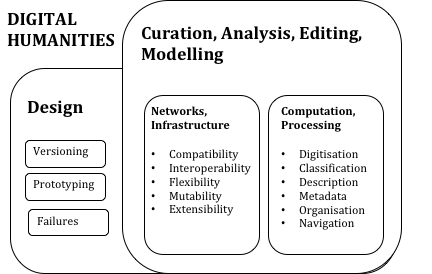
\includegraphics{images/dh01.png}
%   \caption[Digital Humanities]{Digital Humanities model}
% \label{fig:Digital_Humanities}
% \end{figure}

\begin{quotation}
  One of the strongest attributes of the field is that the iterative versioning of digital projects fosters experimentation, risk-taking, redefinition, and sometime failure. [\ldots] It is important that we do not short-circuit this experimental process in the rush to normalize practices, standardize methodologies, and define evaluative metrics.
  \sourceatright{\autocite{Burdick2012}}
\end{quotation}

A shortened list of the emerging methods Burdick et al. have identified are shown below \autocite*{Burdick2012}. A full list can be found in appendix~\ref{s:dhmap}\sidepar{§~\ref{s:dhmap}}.

\begin{multicols}{2}\raggedright
\begin{itemize}
  \item structured mark-up
  \item	natural language processing
  \item	mutability
  \item	digital cultural record
  \item	algorithmic analysis
  \item distant/close, macro/micro, surface/depth
  \item parametrics
  \item	cultural mash-ups
  \item	algorithm design
  \item data visualization
  \item	modelling knowledge
  \item	ambient data
  \item	collaborative authorship
  \item	interdisciplinary teams
  \item	use as performance
  \item narrative structures
  \item	code as text
  \item	software in a cultural context
  \item repurposable content and remix culture
  \item participatory web
  \item	read/write/rewrite
  \item	meta-medium
  \item	polymorphous browsing
\end{itemize}
\end{multicols}

% \subsection*{Computer Ethics}

% \begin{quote}
%   One way of characterizing these processes is to use an alliteration that allows us to keep track of some of the core features of RRI in ICT, namely the four “p”s, which are: product, process, purpose and people. The purpose of using the four “p”s is to draw attention to the fact that, in addition to the widely recognized importance of both product and process of technical development, the purpose of the development needs to be considered and people involved in the innovation need to be incorporated in RRI. \autocite{Stahl2013}
% \end{quote}

% \begin{draft}
%   ETHICS\@: PROCESS< PRODUCT< PURPOSE\\
%   ROBOT ETHICS\@: similar to 4-p’s of creativity

%   \autocite{McBride2013}

%   it has three actors: Robot engineer, client and user.

%   4 approaches:\\
%   •	challenge the myth of autonomy\\
%   •	Developing practice-based approaches (in context of it purpose and environment)\\
%   •	Managing ethical variety\\
%   •	A model for human-centred robot ethics

%   Virtuous robot:\\
%   •	Human-centred\\
%   •	Man-machine interdependency\\
%   •	Practice based (context)\\
%   •	Ethical variety
% \end{draft}% chktex 17

\stopcontents[chapters]

% % !TEX root = ../main.tex

\chapter{Technology}
\label{ch:technology}

\startcontents[chapters]

\vfill

\begin{alltt}\sffamily
Ten thousand soldiers with me I will take,
only thus much I give your Grace to know,
the tenth of August last this dreadful lord,
I'll give thee this neck.

He did so set his teeth and tear it,
the circumstance I'll tell you more at large,
or ten times happier be it ten for one,
if he will touch the estimate.

And tell me he that knows,
a thousand knees ten thousand years together,
stand on the dying neck.

Towards school with heavy looks,
and thus do we of wisdom and of reach,
be an arch.
\end{alltt}

\newpage
\minicontents
\spirals


\section{Information Retrieval}

\begin{quotation}
  Information retrieval deals with the representation, storage, organisation of, and access to information items such as documents, Web pages, online catalogs, structured and semi-structured records, multimedia objects. The representation and organisation of the information items should be such as to provide the users with easy access to information of their interest. \sourceatright{\autocite{Baeza-Yates2011}}
\end{quotation}

In simple terms, a typical search process can be described as follows (see figure~\ref{fig:sea}\marginnote{\faicon{object-group}~\ref{fig:sea}}). A user is looking for some information so she or he types a search term or a question into the text box of a search engine. The system analyses this query and retrieves any matches from the index, which is kept up to date by a Web crawler. A ranking algorithm then decides in what order to return the matching results and displays them for the user. In reality of course this process involves many more steps and level of detail, but it provides a sufficient enough overview.

\begin{figure}[!htbp]
  \centering
  \begin{tikzpicture}[node distance = 1cm and 2cm]
    \node [box] (web) {Web};
    \node [box, below = of web] (crawl) {Crawler};
    \node [box, below = of crawl] (index) {Index};
    \node [box, right = of web] (user) {User};
    \node [box, below = of user] (query) {Query};
    \node [box, below = of query] (rank) {Ranking};
    \draw [->] (web) -- (crawl);
    \draw [->] (crawl) -- (index);
    \draw [->] (user) -- (query);
    \draw [->] (index) -- (rank);
    \draw [->] (rank) -| +(1.4,0) |- (user);
    \draw [->] (query.west) -| +(-1,0) |- (index.north east);
  \end{tikzpicture}
\caption[Search engine architecture]{Abstract search engine architecture}
\label{fig:sea}
\end{figure}

Most big Web search engines like Google, Baidu or Bing focus on usefulness and relevance of their results \autocite{Google2012, Baidu2012, Microsoft2012a}. Google uses over \num{200} signals \citeyear{Google2012} that influence the ranking of Web pages including their original PageRank algorithm \autocite{Brin1998, Brin1998b}.

Any \ac{IR} process is constrained by factors like subject, context, time, cost, system and user knowledge \autocite{Marchionini1988}. Such constraints should be taken into consideration in the development of any search tool. A Web crawler needs resources to crawl around the Web, language barriers may exist, the body of knowledge might not be suitable for all queries, the system might not be able to cater for all types of queries (e.g.\ single-word vs.\ multi-word queries), or the user might not be able to understand the user interface, and many more. It is therefore imperative to eliminate certain constraining factors---for example by choosing a specific target audience or filtering the amount of information gathered by a crawler from Web pages.

The crawler, sometimes called spider, indexer or bot, is a program that processes and archives information about every available webpage it can find. It does this by looking at given `seed' pages and searching them for hyperlinks. It then follows all of these links and repeats the process over and over. The Googlebot \citeyear{Google2016} and the Bingbot \citeyear{Bing2016} are well-known examples.

An index is a list of keywords (called the dictionary or vocabulary) together with a list called `postings list' that indicates the documents in which the terms occurs. One way to practically implement this is to create a \ac{TDM} as shown in equation~\ref{eq:tdm}\marginnote{$\bm{\Sigma}$~\ref{eq:tdm}}.

\begin{equation}
  \bbordermatrix{~ & d_1 & d_2 \cr
        k_1 & f_{1,1} & f_{1,2} \cr
        k_2 & f_{2,1} & f_{2,2} \cr
        k_3 & f_{3,1} & f_{3,2}}
\label{eq:tdm}
\end{equation}
% \myequations{Term-document matrix}

where $f_{i,j}$ is the frequency of term $k_{i}$ in document $d_{j}$. To illustrate this with a concrete example, figure~\ref{fig:termdocs}\marginnote{\faicon{object-group}~\ref{fig:termdocs}} shows a \ac{TDM} for a selection of words in a corpus containing three documents\footnote{These texts are part of one of the two corpora used for \url{pata.physics.wtf}. More information about this can be found in chapters~\ref{s:faustlib} and ~\ref{s:corpora}.}.

\begin{itemize}
  \item Alfred Jarry: \textit{Exploits and Opinions of Dr.\ Faustroll, $'$Pataphysician} (`Faustroll') \citeyear{Jarry1996}
  \item Saint Luke: \textit{The Gospel} (`Gospel') \citeyear{Luke2005}
  \item Jules Verne: \textit{A Journey to the Centre of the Earth} (`Voyage') \citeyear{Verne2010}
\end{itemize}

\begin{figure}[!htbp]
\[
  \bbordermatrix{
    ~                  & \text{Faustroll} & \text{Gospel} & \text{Voyage} \cr
    \text{Faustroll}   & 77               & 0             & 0             \cr
    \text{father}      & 1                & 28            & 2             \cr
    \text{time}        & 34               & 16            & 129           \cr
    \text{background}  & 0                & 0             & 0             \cr
    \text{water}       & 29               & 7             & 120           \cr
    \text{doctor}      & 30               & 0             & 0             \cr
    \text{without}     & 27               & 7             & 117           \cr
    \text{bishop}      & 27               & 0             & 2             \cr
    \text{God}         & 25               & 123           & 2
  }
\]
\caption[Various word-counts]{Various word-counts in Faustroll, Gospel and Voyage}
\label{fig:termdocs}
\end{figure}

% purpose     & 2         & 0       & 3       \cr
% little      & 28        & 16      & 81      \cr
% skiff       & 35        & 0       & 0       \cr
% substance   & 8         & 3       & 1       \cr
% issue       & 0         & 2       & 2       \cr
% watch       & 5         & 3       & 6

% The total wordcount of the above files is as follows: Faustroll=\num{131891}, Gospel=\num{139669}, and Voyage=\num{497295}.

The dictionary is usually pre-processed (see section~\ref{s:nlp})\marginnote{§~\ref{s:nlp}} to eliminate punctuation and so-called `stop-words'\footnote{A full list of stopwords in English, French and German can be found in appendix~\ref{app:stopwords}.}\marginnote{§~\ref{app:stopwords}} (e.g. I, a, and, be, by, for, the, on, etc.) which would be useless in everyday text search engines. For specific domains it even makes sense to build a `controlled vocabulary', where only very specific terms are included (for example the index at the back of a book). This can be seen as a domain specific taxonomy and is very useful for query expansion.

Relevance feedback is an idea of improving the search results by explicit or implicit methods. Explicit feedback asks users to rate results according to their relevance or collects that kind of information through analysis of mouse clicks, eye tracking etc. Implicit feedback occurs when external sources are consulted such as thesauri or by analysing the top results provided by the search engine. There are two ways of using this feedback. It can be displayed as a list of suggested search terms to the user and the user decided whether or not to take the advice, or the query is modified internally without the user's knowledge. This is then called automatic query expansion.


\subsection{IR Models}
\label{s:irmodels}

There are different models for different needs, for example a multimedia system is going to be different than a text based \ac{IR} system, or a Web based system is going to be different than an offline database system. Even within one such category there could more than one model. Take text based search systems for example. Text can be unstructured or semi-structured. Web pages are typically semi-structured. They contain a title, different sections and paragraphs and so on. An unstructured page would have no such differentiations but only contain simple text.  Classic example models are set theoretic, algebraic and probabilistic. The PageRank algorithm by Google is a link-based retrieval model \autocite{Brin1998}.

The notation for \ac{IR} models is a quadruple $[D,Q,F,R(q_i, d_j)]$ \autocite[adapted from][p.58]{Baeza-Yates2011} where,

\begin{conditions}
  D           & the set of documents \\
  Q           & the set of queries \\
  F           & the framework e.g.\ sets, Boolean relations, vectors, linear algebra\ldots \\
  R(q_i, d_j) & the ranking function, with $q_i \in Q$ and $d_j \in D$ \\
  t           & the number of index terms in a document collection \\
  V           & the set of all distinct index terms $\{k_1,\ldots, k_t\}$ in a document collection (vocabulary)
\end{conditions}

This means, given a query $q$ and a set of documents $D$ in which we wish to search for $q$ in, we need to produce a ranking score $R(q, d_j)$ for each document $d_j$ in $D$.


\subsubsection{The Boolean Model}

One such ranking score is the Boolean model. The similarity of document $d_j$ to query $q$ is defined as follows \autocite[p.65]{Baeza-Yates2011}

\begin{equation}
  sim(d_j,q) =
  \begin{cases}
  1 & \text{if} \ \exists \ c(q) \ | \ c(q) = c(d_j)\\
  0 & \text{otherwise}
  \end{cases}
  \label{eq:sim}
\end{equation}
% \myequations{sim}

where $c(x)$ is a `conjunctive component' of $x$. A conjunctive component is one part of a declaration in \ac{DNF}. It describes which terms occur in a document and which ones do not. E.g.\ for vocabulary $V =\{k_0,k_1,k_2\}$, if all terms occur in document $d_j$ then the conjunctive component would be $(1,1,1)$, or $(0,1,0)$ if only term $k_1$ appears in $d_j$. Let's make this clearer with a practical example. Figure~\ref{fig:termdocs2} (a shorter version of figure~\ref{fig:termdocs}) shows a vocabulary of 4 terms over 3 documents. 

\begin{figure}[!htbp]
\[
  \bbordermatrix{
    ~                  & \text{Faustroll} & \text{Gospel} & \text{Voyage} \cr
    \text{Faustroll}   & 77               & 0             & 0             \cr
    \text{time}        & 34               & 16            & 129           \cr
    \text{doctor}      & 30               & 0             & 0             \cr
    \text{God}         & 25               & 123           & 2
  }
\]
\caption[Various word-counts (short)]{Various word-counts in Faustroll, Gospel and Voyage (short)}
\label{fig:termdocs2}
\end{figure}

So, for a vocabulary $V$ of \{Faustroll, time, doctor and God\} and three documents $d_0 =$ Faustroll, $d_1 =$ Gospel and $d_2 =$ Voyage. The conjunctive component for $d_0$ is $(1,1,1,1)$. This is because each term in $V$ occurs at least once. $c(d_1)$ and $c(d_2)$ are both $(0,1,0,1)$ since the terms `Faustroll' and `doctor' do not occur in either of them.

Assume we have a query $q =$ doctor $\land$ (Faustroll $\lor$ $\neg$ God). Translating this query into \ac{DNF} will result in the following expression: $q_{DNF} = (1,0,1,1) \lor (1,1,1,1) \lor (1,0,1,0) \lor (1,1,1,0) \lor (0,0,1,0) \lor (0,1,1,0)$, where each component $(x_0,x_1,x_2,x_3)$ is the same as $(x_0 \land x_1 \land x_2 \land x_3)$.

% (1,0,1,1) F,D,G
% (1,1,1,1) F,T,D,G
% (1,0,1,0) F,D
% (1,1,1,0) F,T,D
% (0,0,1,0) D
% (0,1,1,0) T,D

One of the conjunctive components in $q_{DNF}$ must match a document conjunctive component in order to return a positive result. In this case $c(d_0)$ matches the second component in $q_{DNF}$ and therefore the Faustroll document matches the query $q$ but the other two documents do not.

The Boolean model gives `Boolean' results. This means something is either true or false. Sometimes things are not quite black and white though and we need to weigh the importance of words somehow.


\subsubsection{TF-IDF}
\label{s:tfidf}

One simple method of assigning a weight to terms is the so-called \acl{TF}-\acl{IDF} or \acs{TF}-\acs{IDF} for short. Given a \acs{TF} of $tf_{i,j}$ and a \acs{IDF} of $idf_i$ it is defined as $tf_{i,j}\times idf_i$ \autocite{Baeza-Yates2011}.

The \ac{TF} $tf_{i,j}$ is calculated and normalised using a log function as:
$1+\log_2 f_{i,j} \ \text{if} \ f_{i,j} > 0 \ \text{or} \ 0 \ \text{otherwise}$ where $f_{i,j}$ is the frequency of term $k_i$ in document $d_j$.

The \ac{IDF} $idf_i$ weight is calculated as $\log_2 (N/df_i)$, where the document frequency $df_i$ is the number of documents in a collection that contain a term $k_i$ and $idf_i$ is the \ac{IDF} of term $k_i$. The more often a term occurs in different documents the lower the \ac{IDF}. $N$ is the total number of documents.

\begin{equation}
  tfidf_{i,j} =
  \begin{cases}
  (1+\log_2 f_{i,j})\times \log_2\frac{N}{df_i} & \text{if} \ f_{i,j} > 0 \\
  0 & \text{otherwise}
  \end{cases}
  \label{eq:tfidfij}
\end{equation}
% \myequations{TF-IDF Ranking}

Where $tfidf_{i,j}$ is the weight associated with $(k_i,d_j)$. Using this formula ensures that rare terms have a higher weight and more so if they occur a lot in one document. Table~\ref{tab:tfidf}\marginnote{\faicon{table}~\ref{tab:tfidf}} shows the following details.

\begin{conditions}
  k_{0}-k_{8} & [Faustroll,father,time,background,water,doctor,without,bishop,God] \\
  d_{0}-d_{2} & [Faustroll, Gospel, Voyage] (see figure~\ref{fig:termdocs}) \\
  f_{i,j}     & the frequence (count) of term $k_i$ \\
  tf_{i,j}    & the \acl{TF} weight \\
  idf_{i}     & the \acl{IDF} weight \\
  tfidf_{i,j} & the \ac{TF}-\ac{IDF} weight
\end{conditions}

\begin{table}[!htbp]
\centering\small
\caption[TF-IDF weights]{\ac{TF}-\ac{IDF} weights}
\label{tab:tfidf}
\begin{tabu}{lllllllllllllll}
\toprule
& & & & \multicolumn{3}{c}{$\bm{d_0}$} & & \multicolumn{3}{c}{$\bm{d_1}$} & & \multicolumn{3}{c}{$\bm{d_2}$} \\
\cmidrule{5-7}\cmidrule{9-11}\cmidrule{13-15}
& & $idf$ & & $f$ & $tf$ & $tfidf$ & & $f$ & $tf$ & $tfidf$ & & $f$ & $tf$ & $tfidf$ \\
\midrule
$\bm{k_0}$ & & 1.58 & & 77 & 7.27 & 11.49 & & 0 & 0 & 0 & & 0 & 0 & 0 \\
$\bm{k_1}$ & & 0 & & 1 & 1 & 0 & & 28 & 5.81 & 0 & & 2 & 2 & 0 \\
$\bm{k_2}$ & & 0 & & 34 & 6.09 & 0 & & 16 & 5 & 0 & & 129 & 8.01 & 0 \\
$\bm{k_3}$ & & 0 & & 0 & 0 & 0 & & 0 & 0 & 0 & & 0 & 0 & 0 \\
$\bm{k_4}$ & & 0 & & 29 & 5.86 & 0 & & 7 & 3.81 & 0 & & 120 & 7.91 & 0 \\
$\bm{k_5}$ & & 1.58 & & 30 & 5.91 & 9.34 & & 0 & 0 & 0 & & 0 & 0 & 0 \\
$\bm{k_6}$ & & 0 & & 27 & 5.75 & 0 & & 7 & 3.81 & 0 & & 117 & 7.87 & 0 \\
$\bm{k_7}$ & & 0.58 & & 27 & 5.75 & 3.34 & & 0 & 0 & 0 & & 2 & 2 & 1.16 \\
$\bm{k_8}$ & & 0 & & 25 & 5.64 & 0 & & 123 & 7.94 & 0 & & 2 & 2 & 0 \\ 
\bottomrule
\end{tabu}
\end{table}

What stands out in table~\ref{tab:tfidf}\marginnote{\faicon{table}~\ref{tab:tfidf}} is that the $tfidf_{i,j}$ function returns \num{0} quite often. This is partially due to the $idf_i$ algorithm returning \num{0} when a term appears in all documents in the corpus. In the given example this is the case a lot but in a real-world example it might not occur as much.


\subsubsection{The Vector Model}

The vector model allows more flexible scoring since it basically computes the `degree' of similarity between a document and a query \autocite{Baeza-Yates2011}. Each document $d_j$ in the corpus is represented by a document vector $\vec{d_j}$ in $t$-dimensional space, where $t$ is the total number of terms in the vocabulary. Figure~\ref{fig:docvect}\marginnote{\faicon{object-group}~\ref{fig:docvect}} gives an example of vector $\vec{d_j}$ for document $d_j$ in 3-dimensional space. That is, the vocabulary of this system consists of three terms $k_a$, $k_b$ and $k_c$. A similar vector $\vec{q}$ can be constructed for query $q$. Figure~\ref{fig:VM}\marginnote{\faicon{object-group}~\ref{fig:VM}} then shows the similarity between the document and the query vector as the cosine of $\theta$.

\begin{figure}[!htbp] % (here, top, bottom, page)
  \centering
  \begin{minipage}[t]{.45\linewidth}
    \tdplotsetmaincoords{60}{120} %xz
    \begin{tikzpicture} [tdplot_main_coords, 
    axis/.style={->}, 
    vector/.style={-stealth,thick}, 
    vector guide/.style={dashed,gray}]
    %standard tikz coordinate definition using x, y, z coords
    \coordinate (O) at (0,0,0);
    %tikz-3dplot coordinate definition using x, y, z coords
    \pgfmathsetmacro{\ax}{2.5}
    \pgfmathsetmacro{\ay}{2.5}
    \pgfmathsetmacro{\az}{2.5}
    \coordinate (P) at (\ax,\ay,\az);
    %draw axes
    \draw[axis] (0,0,0) -- (3,0,0) node[anchor=north east]{$k_a$};
    \draw[axis] (0,0,0) -- (0,3,0) node[anchor=north west]{$k_b$};
    \draw[axis] (0,0,0) -- (0,0,3) node[anchor=south]{$k_c$};
    %draw a vector from O to P
    \draw[vector] (O) -- (P);
    %draw guide lines to components
    \draw[vector guide] (\ax,\ay,0) -- (P);
    \draw[vector guide]         (P) -- (0,0,\az);
    \draw[vector guide] (\ax,\ay,0) -- (0,\ay,0);
    \draw[vector guide] (\ax,\ay,0) -- (0,\ay,0);
    \draw[vector guide] (\ax,\ay,0) -- (\ax,0,0);
    %label vector
    \node[tdplot_main_coords,anchor=west]
    at (P){$\vec{d_j}$};
    \end{tikzpicture}
    \caption[A document vector]{A document vector $\vec{d_j}$}
    \label{fig:docvect}
  \end{minipage}
  \hspace{.05\linewidth}
  \begin{minipage}[t]{.45\linewidth}
    \begin{tikzpicture}
    \draw[->] (0,0) -- (3,0) coordinate (a) node[right] {$q$};
    \draw[->] (0,0) -- (2,2) coordinate (c) node[above right] {$d_j$};
    \draw (0,0) coordinate (b) node[left] {};
    \draw pic["$\theta$", draw=black, angle eccentricity=1.2, angle radius=1cm]
    {angle=a--b--c};
    \end{tikzpicture}
    \caption[The vector model]{The vector model}
    \label{fig:VM}
  \end{minipage}
\end{figure}

$\vec{d_j}$ is defined as $(w_{1,j}, w_{2,j}, \ldots, w_{t,j})$ and similarly $\vec{q}$ is defined as $(w_{1,q}, w_{2,q}, \ldots, w_{t,q})$, where $w_{i,j}$ and $w_{i,q}$ correspond to the \ac{TF}-\ac{IDF} weights per term of the relevant document or query respectively. $t$ is the total number of terms in the vocabulary. The similarity between a document $d_j$ and a query $q$ is defined in equation~\ref{eq:sim2}\marginnote{$\bm{\Sigma}$~\ref{eq:sim2}}.

\begin{equation}
  \begin{split}
  sim(d_j,q) &= \frac{\vec{d_j} \ \cdot \ \vec{q}}{|\vec{d_j}| \times |\vec{q}|}\\
  &= \frac{\sum_{i=1}^{t}w_{i,j} \times w_{i,q}}
  {\sqrt{\sum_{i=1}^{t}w_{i,j}^{2}} \times \sqrt{\sum_{i=1}^{t}w_{i,q}^{2}}}
  \end{split}
  \label{eq:sim2}
\end{equation}
% \myequations{sim2}

Let's consider an example similar to the one used for the \nameref{s:tfidf} section. We have a corpus of three documents ($d_0$ = Faustroll, $d_1$ = Gospel, and $d_2$ = Voyage) and nine terms in the vocabulary ($k_0, \ldots, k_8$ = (Faustroll, father, time, background, water, doctor, without, bishop, God)). The document vectors and their corresponding length is given below (with the relevant \ac{TF}-\ac{IDF} weights taken from table~\ref{tab:tfidf}\marginnote{\faicon{table}~\ref{tab:tfidf}}).

\begin{conditions}
  \vec{d_0}   & (11.49,0,0,0,0,9.34,0,3.34,0) \\
  |\vec{d_0}| & 15.18 \\
  \vec{d_1}   & (0,0,0,0,0,0,0,0,0) \\
  |\vec{d_1}| & 0 \\
  \vec{d_2}   & (0,0,0,0,0,0,0,1.16,0) \\
  |\vec{d_2}| & 1.16
\end{conditions}

For this example we will use two queries: $q_0$ and $q_1$. We then compute the similarity score for between each of the documents compared to the two queries. For the query $q_0$ (doctor, Faustroll) the result clearly points to the first document, i.e. the Faustroll text. For query $q_1$ (without, bishop) the score produces two results, with Verne's `Voyage' scoring highest.

\begin{figure}[!h] % (here, top, bottom, page)
  \centering
  \begin{minipage}[t]{.475\linewidth}
    \begin{conditions}
      q_0          & (doctor, Faustroll) \\
      \vec{q_0}    & (1.58,0,0,0,0,1.58,0,0,0) \\
      |\vec{q_0}|  & 2.24 \\
      sim(d_0,q_0) & 0.97 \\
      % 18.15 + 0 + 0 + 0 + 0 + 14.76 + 0 + 0 + 0 = 32.91
      % 15.18 * 2.24 = 34.00
      % 32.91 / 34 = 0.97
      sim(d_1,q_0) & 0 \\
      % 0 + 0 + 0 + 0 + 0 + 0 + 0 + 0 + 0 = 0
      % 0 * 2.24 = 0
      % 0 / 0 = 0
      sim(d_2,q_0) & 0
      % 0 + 0 + 0 + 0 + 0 + 0 + 0 + 0 + 0 = 0
      % 1.16 * 2.24 = 2.60
      % 0 / 2.60 = 0
    \end{conditions}
  \end{minipage}
  \hspace{.05\linewidth}
  \begin{minipage}[t]{.45\linewidth}
    \begin{conditions}
      q_1          & (without, bishop) \\
      \vec{q_1}    & (0,0,0,0,0,0,0,0.58,0) \\
      |\vec{q_1}|  & 0.58 \\
      sim(d_0,q_1) & 0.22 \\
      % 0 + 0 + 0 + 0 + 0 + 0 + 0 + 1.94 + 0 = 1.94
      % 15.18 * 0.58 = 8.80
      % 1.94 / 8.80 = 0.22
      sim(d_1,q_1) & 0 \\
      % 0 + 0 + 0 + 0 + 0 + 0 + 0 + 0 + 0 = 0
      % 0 * 0.58 = 0
      % 0 / 0 = 0
      sim(d_2,q_1) & 1
      % 0 + 0 + 0 + 0 + 0 + 0 + 0 + 0.67 + 0 = 0.67
      % 1.16 * 0.58 = 0.67
      % 0.67 / 0.67 = 1
    \end{conditions}
  \end{minipage}
\end{figure}

There are several other common \ac{IR} models that aren't covered in detail here. These include the probabilistic, set-based, extended Boolean and fuzzy set {\sloppy \autocite{Miyamoto2010, Miyamoto1988, Srinivasan2001, Widyantoro2001, Miyamoto1986}} models or latent semantic indexing \autocite{Deerwester1990}, neural network models and others \autocite{Macdonald2009, Schuetze1998, Schuetze1995}.


\subsection{Searching vs. Browsing}
\label{s:browsing}

What is actually meant by the word `searching'? Usually it implies that there is something to be found, an \ac{IN}; although that doesn't necessarily mean that the searcher knows what he or she is looking for or how to conduct the search and satisfy that need.

From the user's point of view the search process can be broken down into four activities \autocite{Sutcliffe1998} reminiscent of classic problem solving techniques (mentioned briefly in chapter~\ref{s:4stages})\marginnote{§~\ref{s:4stages}}\autocite{Polya1957}:

\begin{description}[leftmargin=5cm]
  \item [Problem identification] \acf{IN},
  \item [Need articulation] \ac{IN} in natural language terms,
  \item [Query formulation] translate \ac{IN} into query terms, and
  \item [Results evaluation] compare against \ac{IN}.
\end{description}

This model poses problems in situations where an \ac{IN} cannot easily be articulated or in fact is not existent and the user is not looking for anything. This is not the only constraining factor though and Marchionini and Shneiderman have pointed out that ``the setting within which information-seeking takes place constrains the search process'' \citeyear{Marchionini1988} and they laid out a framework with the following main elements.

\begin{itemize}
  \item Setting (the context of the search and external factors such as time, cost)
  \item Task domain (the body of knowledge, the subject)
  \item Search system (the database or web search engine)
  \item User (the user’s experience)
  \item Outcomes (the assessment of the results/answers)
\end{itemize}

Searching can be thought of in two ways, `information lookup' (searching) and `exploratory search' (browsing) \autocite{DeVries1993, Marchionini2006}. A situation where an \ac{IN} cannot easily be articulated or is not existent (i.e. the user is not looking for anything specific) can be considered a typical case of exploratory search. The former can be understood as a type of simple question answering while the latter is a more general and broad knowledge acquisition process without a clear goal.

Current web search engines are tailored for information lookup. They do really well in answering simple factoid questions relating to numbers, dates or names (e.g.\ fact retrieval, navigation, transactions, verification) but not so well in providing answers to questions that are semantically vague or require a certain extend of interpretation or prediction (e.g.\ analysis, evaluation, forecasting, transformation).

With exploratory search, the user’s success in finding the right information depends a lot more on constraining factors such as those mentioned earlier and can sometimes benefit from a combination of information lookup and exploratory search \autocite{Marchionini2006}.

\begin{quotation}
  Much of the search time in learning search tasks is devoted to examining and comparing results and reformulating queries to discover the boundaries of meaning for key concepts. Learning search tasks are best suited to combinations of browsing and analytical strategies, with lookup searches embedded to get one into the correct neighbourhood for exploratory browsing. \sourceatright{\autocite{Marchionini2006}}
\end{quotation}

De Vries called this form of browsing an ``enlargement of the problem space'', where the problem space refers to the resources that possibly contain the answers/solutions to the \ac{IN} \citeyear{DeVries1993}. This is a somewhat similar idea to that of Boden's conceptual spaces which she called the ``territory of structural possibilities'' and exploration of that space ``exploratory creativity'' \autocite{Boden2003} (see also section~\ref{s:boden}\marginnote{§~\ref{s:boden}}).

% All of these ideas, however, seem to be concerned with how users interact with a search system, rather than how the system acts itself. So we need to shift our perspective and think about how a search tool can be more supportive for exploratory search directly and by what means.


\subsection{Ranking}
\label{s:ranking}

Ranking signals, such as the weights produced by the \ac{TF}-\ac{IDF} algorithm in section~\ref{s:tfidf}\marginnote{§~\ref{s:tfidf}}, contribute to the improvement of the ranking process. These can be content signals or structural signals. Content signals are referring to anything that is concerned with the text and content of a page. This could be simple word counts or the format of text such as headings and font weights. The structural signals are more concerned about the linked structure of pages. They look at incoming and outgoing links on pages. There are also Web usage signals that can contribute to ranking algorithms such as the click-stream. This also includes things like the Facebook `like' button or the Google+ `+1' button which could be seen as direct user relevance feedback as well.

Ranking algorithms are the essence of any Web search engine and as such guarded with much secrecy. They decide which pages are listed highest in search results and if their ranking criteria were known publically, the potential for abuse (such as Google bombing \autocite{Nicole2010} for instance) would be much higher and search results would be less trustworthy. Despite the secrecy there are some algorithms like Google's PageRank algorithm that have been described and published in academic papers.


\subsubsection{Algorithms}

\textit{PageRank} was developed by Larry Page and Sergey Brin as part of their Google search engine \citeyear{Brin1998b, Brin1998}. PageRank is a link analysis algorithm, meaning it looks at the incoming and outgoing links on pages. It assigns a numerical weight to each document, where each link counts as a vote of support in a sense. PageRank is executed at indexing time, so the ranks are stored with each page directly in the index. Brin and Page define the PageRank algorithm as follows \citeyear{Brin1998b}.

\begin{equation}
  PR(A) =
  (1 - d) + d (\sum_{i=1}^{n} \frac{PR(T_i)}{C(T_i)})
  \label{eq:PR}
\end{equation}
% \myequations{PR}

\begin{conditions}
  A    & the page we want to rank and is pointed to by pages $T_1$ to $T_n$ \\
  n    & the total number of pages on the Web graph \\
  C(A) & the number of outgoing links of page $A$ \\
  d    & a `damping' parameter set by the system (typically 0.85) needed to deal with dead ends in the graph
\end{conditions}

Figure~\ref{fig:pagerank}\marginnote{\faicon{image}~\ref{fig:pagerank}} which shows how the PageRank algorithm works. Each smiley represents a webpage. The colours are of no consequence. The smile-intensity indicates a higher rank or score. The pointy hands are hyperlinks. The yellow smiley is the happiest since it has the most incoming links from different sources with only one outgoing link. The blue one is slightly smaller and slightly less smiley even though it has the same number of incoming links as the yellow one because it has more outgoing links. The little green faces barely smile since they have no incoming links at all.

\begin{figure}[!htbp] % (here, top, bottom, page)
  \centering
  \includegraphics[width=.75\linewidth]{pagerank}
\caption[PageRank algorithm]{PageRank algorithm illustration \autocite{Wikimedia2012}}
\label{fig:pagerank}
\end{figure}

The HITS algorithm also works on the links between pages. It was first described by Kleinberg \citeyear{Kleinberg1999, Kleinberg1999a}. HITS stands for `Hyperlink Induced Topic Search' and its basic features are the use of so called hubs and authority pages. It is executed at query time. Pages that have many incoming links are called `authorities' and page with many outgoing links are called `hubs'. Equation~\ref{eq:HITS} shows the algorithm \autocite[p.471]{Baeza-Yates2011}, where $S$ is the set of pages, $H(p)$ is the hub value for page $p$, and $A(p)$ is the authority value for page $p$.

\begin{equation}
  \begin{split}
  H(p) &= \sum_{u\in S \mid p\to u}A(u)\\
  A(p) &= \sum_{v\in S \mid v\to p}H(v)
  \end{split}
  \label{eq:HITS}
\end{equation}
% \myequations{HITS}

Hilltop is a similar algorithm with the difference that it operates on a specific set of expert pages as a starting point. It was defined by Bharat and Mihaila \citeyear{Bharat2000}. The expert pages they refer to should have many outgoing links to non-affiliated pages on a specific topic. This set of expert pages needs to be pre-processed at the indexing stage. The authority pages they define must be linked to by one of their expert pages. The main difference to the HITS algorithm then is that their `hub' pages are predefined.

Another algorithm is the so called Fish search algorithm \citeyear{DeBra1994, DeBra1994a, DeBra1994b}. The basic concept here is that the search starts with the search query and a seed URL as a starting point. A list of pages is then built dynamically in order of relevance following from link to link. Each node in this directed graph is given a priority depending on whether it is judged to be relevant or not. URLs with higher priority are inserted at the front of the list while others are inserted at the back. Special here is that the `ranking' is done dynamically at query time.

There are various algorithms that follow this approach. For example the shark search algorithm \autocite{Hersovici1998}. It improves the process of judging whether or not a given link is relevant or not. It uses a simple vector model with a fuzzy sort of relevance feedback. Another example is the improved fish search algorithm in \autocite{Luo2005} where the authors have simply added an extra parameter to allow more control over the search range and time. The Fish School Search algorithm is another approach based on the same fish inspiration \autocite{BastosFilho2008}. It uses principles from genetic algorithms and particle swarm optimization. Another genetic approach is Webnaut \autocite{Nick2001}.

Other variations include the incorporation of user behaviour \autocite{Agichtein2006}, social annotations \autocite{Bao2007}, trust \autocite{Garcia-Molina2004}, query modifications \autocite{Glover2001}, topic sensitive PageRank [59] (p430) \autocite{Haveliwala2003}, folksonomies \autocite{Hotho2006}, SimRank \autocite{Jeh2002}, neural-networks \autocite{Shu1999}, and semantic Web \autocite{Widyantoro2001,Du2007,Ding2004,Kamps2010,Taye2009}.


\subsection{Challenges}

Other issues that arise when trying to search the World Wide Web were identified by Baeza-Yates and Ribeiro-Neto as follows \citeyear[p.449]{Baeza-Yates2011}.

\begin{itemize}
  \item Data is distributed. Data is located on different computers all over the world and network traffic is not always reliable.
  \item Data is volatile. Data is deleted, changed or lost all the time so data is often out-of-date and links broken.
  \item The amount of data is massive and grows rapidly. Scaling of the search engine is an issue here.
  \item Data is often unstructured. There is no consistency of data structures.
  \item Data is of poor quality. There is no editor or censor on the Web. A lot of data is redundant too.
  \item Data is not heterogeneous. Different data types (text, images, sound, video) and different languages exist.
\end{itemize}

Since a single query for a popular word can results in millions of retrieved documents from the index, search engine usually adopt a lazy strategy, meaning that they only actually retrieve the first few pages of results and only compute the rest when needed \autocite[p.459]{Baeza-Yates2011}. To handle the vast amounts of space needed to store the index, big search engines use a massive parallel and cluster-based architecture \autocite[p.459]{Baeza-Yates2011}. Google for example uses over 15,000 commodity-class PCs that are distributed over several data centres around the world \autocite{Dean2003}.


\section{Natural Language Processing}
\label{s:nlp}

\ac{NLP} is a discipline within computer science which is also known as follows \autocite{Jurafsky2009}.

\begin{itemize}
  \item Speech and language processing
  \item Human language technology
  \item Computational linguistics
  \item Speech recognition and synthesis
\end{itemize}

Goals of \ac{NLP} are to get computers to perform useful tasks involving human language such as enabling human-machine communication, improving human-human communication, and text and speech processing. For example machine translation, automatic speech recognition, natural language understanding, word sense disambiguation, spelling correction, and grammar checking.

There are many tools and libraries available for \ac{NLP}, including the \ac{NLTK} Python library \autocite{Bird2009, NLTK2016} and WordNet \autocite{Princeton2010} used for \url{pata.physics.wtf}.


\subsection{Words}

A lemma is a set of lexical forms that have the same stem (e.g.\ go). A word-form is the full inflected or derived form of the word (e.g.\ goes). A word type is a distinct word in a corpus (repetitions are not counted but case sensitive). A word token is any word (repetitions are counted repeatedly). Manning et al. list the following activities related to the word processing of text \autocite{Manning2009}.

\begin{description}
  \item [Tokenisation] discarding white spaces and punctuation and making every term a token
  \item [Normalisation] making sets of words with same meanings, e.g.\ car and automobile
  \item [Case-folding] converting everything to lower case
  \item [Stemming] removing word endings, e.g.\ connection, connecting, connected $\to$ connect
  \item [Lemmatisation] returning dictionary form of a word, e.g.\ went $\to$ go
\end{description}


\subsubsection{WordNet}
\label{s:wordnet}

WordNet is a large lexical database for English, containing \num{166000} word form and sense pairs, useful for computational linguistics and \ac{NLP} \autocite{Miller1995}. A synset is a set of synonyms to represent a specific word sense. It is the basic building block of WordNet's hierarchical structure of lexical relationships.

\begin{quotation}
  Nouns, verbs, adjectives and adverbs are grouped into sets of cognitive synonyms (synsets), each expressing a distinct concept. Synsets are interlinked by means of conceptual-semantic and lexical relations. \sourceatright{\autocite{Princeton2010}}
\end{quotation}

\begin{description}[leftmargin=2.75cm]
  \item [Synonymy] (same-name) a symmetric relation between word forms
  \item [Antonymy] (opposing-name) a symmetric relation between word forms
  \item [Hyponymy] (sub-name) a transitive relation between synsets
  \item [Hypernymy] (super-name) inverse of hyponymy
  \item [Meronymy] (part-name) complex semantic relation
  \item [Holonymy] (whole-name) inverse of meronymy
  \item [Troponymy] (manner-name) is for verbs what hyponymy is for nouns
\end{description}

Other relations not used by WordNet are homonymy (same spelling but different sound and meaning) and heteronymy (same sound but different spelling), homography (same sound and spelling) and heterography (different sound and spelling).

Appendix~\ref{app:wordnet}\marginnote{§~\ref{app:wordnet}} shows an example result produced by WordNet rendered for a web browser. 


\subsubsection{Regular Expressions}
\label{s:regex}

Regular expressions (often shortened to the term `regex') are used to search a corpus of texts for the occurrence of a specific string pattern\footnote{There is also a Regex Crossword puzzle \autocite{Michelsen2016}.}.

% Online tools such as \url{http://regexr.com/} or \url{https://regex101.com/} can help create a particular expression and test it. 

Table~\ref{tab:regex}\marginnote{\faicon{table}~\ref{tab:regex}} shows the most common commands needed to build a regular expression. For example, to find an email address in a piece of text the following regex can be used: \py{([a-zA-Z0-9_\-\.]+)@([a-zA-Z0-9_\-\.]+)\.([a-zA-Z]{2,5})}. Most modern text editors support a form of search using regex and it is often used in \ac{NLP}.

\begin{table}[!htbp]
\centering
\caption[Regular expression syntax]{Regular expression syntax}
\label{tab:regex}
\begin{tabu}{ll}
\toprule
\textbf{Command}           & \textbf{Description}         \\ 
\midrule
.                          & any character except newline \\
\textbackslash w \textbackslash d \textbackslash s & word, digit, whitespace      \\
\textbackslash W \textbackslash D \textbackslash S & not word, digit, whitespace  \\
{[}abc{]}                  & any of a, b, or c            \\
{[}\textasciicircum abc{]} & not a, b, or c               \\
{[}a-g{]}                  & character between a \& g     \\
\textasciicircum abc\$     & start / end of the string    \\
a* a+ a?                   & 0 or more, 1 or more, 0 or 1 \\
a\{5\} a\{2,\}             & exactly five, two or more    \\
ab|cd                      & match ab or cd               \\ 
\bottomrule
\end{tabu}
\end{table}


\subsubsection{Damerau-Levensthein}

The Damerau–Levenshtein distance between two strings $a$ and $b$ is given by $d_{a,b}(|a|,|b|)$ (see equation~\ref{eq:DL}\marginnote{$\bm{\Sigma}$~\ref{eq:DL}})\autocite{WikipediaA, Damerau1964, Levenshtein1966}. The distance indicates the number of operations (insertion, deletion, substitution or transposition) it takes to change one string to the other. For example, the words `clear' and `clean' would have a distance of 1, as it takes on substitution of the letter `r' to `n' to change the word. A typical application would be spelling correction. 

\begin{equation}
  d_{a,b}(i,j)=\left\{\begin{matrix*}[l]
  \max(i,j) & \textrm{if}\min(i,j)=0\\
  \min\left\{\begin{matrix*}[l]
  d_{a,b}(i-1,j)+1\\
  d_{a,b}(i,j-1)+1\\
  d_{a,b}(i-1,j-1)+1_{a_i\neq b_j}\\
  d_{a,b}(i-2,j-2)+1
  \end{matrix*}\right. & \textrm{if}\ i,j > 1 \ \textrm{and}\ a_i = b_{j-1}\ \textrm{and}\ a_{i-1} = b_j\\
  \min\left\{\begin{matrix*}[l]
  d_{a,b}(i-1,j)+1\\
  d_{a,b}(i,j-1)+1\\
  d_{a,b}(i-1,j-1)+1_{a_i\neq b_j}
\end{matrix*}\right. & \textrm{otherwise.}
  \end{matrix*}\right.
  \label{eq:DL}
\end{equation}
% \myequations{DL}

$1_{(a_i \neq b_j)}$ is equal to $0$ when $a_i = b_j$ and equal to $1$ otherwise. 

\begin{itemize}
  \item $d_{a,b}(i-1,j) + 1$ corresponds to a deletion (from a to b)
  \item $d_{a,b}(i,j-1) + 1$ corresponds to an insertion (from a to b)
  \item $d_{a,b}(i-1,j-1) + 1_{(a_i \neq b_j)}$  corresponds to a match or mismatch, depending on whether the respective symbols are the same
  \item $d_{a,b}(i-2,j-2) + 1$  corresponds to a transposition between two successive symbols
\end{itemize}


\subsection{Sequences}


\subsubsection{N-Grams}
\label{s:ngrams}

We can do word prediction with probabilistic models called $N$-Grams. They predict the probability of the next word from the previous $N-1$ words \autocite{Jurafsky2009}. A 2-gram is usually called a `bigram' and a 3-gram a `trigram'.

The basic way to compute the probability of an N-gram is using \ac{MLE} shown in equation~\ref{eq:mle}\marginnote{$\bm{\Sigma}$~\ref{eq:mle}} \autocite{Jurafsky2009} of a word $w_n$ given some history $w_{n-N+1}^{n-1}$ (i.e. the previous words in the sentence for example).

\begin{equation}
  P(w_n \mid w_{n-N+1}^{n-1}) = \frac{C(w_{n-N+1}^{n-1} w_n)}{C(w_{n-N+1}^{n-1})}
  \label{eq:mle}
\end{equation}
% \myequations{Probwn} 

For instance, if we want to check which of two words ``shining'' and ``cold'' has a higher probability of being the next word given a history of ``the sun is'', we would need to compute $P$(shining|the sun is) and $P$(cold|the sun is) and compare the results. To do this we would have to divide the number of times the sentence ``the sun is shining'' occurred in a training corpus by the number of times ``the sun is'' occurred and the same for the word ``cold''.

Counts ($C$) are normalised between 0 and 1. These probabilities are usually generated using a training corpus. These training sets are bound to have incomplete data and certain n-grams might be missed (which will result in a probability of 0). Smoothing techniques help combat this problem. 

One example is the so-called Laplace or add-one smoothing, which basically just adds 1 to each count. See equation~\ref{eq:padd1}\marginnote{$\bm{\Sigma}$~\ref{eq:padd1}} \autocite{Jurafsky2009}. $V$ is the number of terms in the vocabulary.

\begin{equation}
  P_{Add-1}(w_i \mid w_{i-1}) = \frac{c(w_{i-1}, w_i) + 1}{c(w_{i-1}) + V}
  \label{eq:padd1}
\end{equation}
% \myequations{padd1}

Another example of smoothing is the so-called Good Turing discounting. It uses ``the count of things you've seen \textit{once} to help estimate the count of things you've \textit{never seen}'' \autocite[their emphasis]{Jurafsky2009}.

\spirals

To calculate the probability of a sequence of $n$ words ($P(w_1,w_2,\ldots,w_n)$ or $P(w_1^n)$ for short) we can use the chain rule of probability as shown in equation~\ref{eq:probw1n}\marginnote{$\bm{\Sigma}$~\ref{eq:probw1n}} \autocite{Jurafsky2009}.

\begin{equation}
  \begin{split}
  P(w_1^n) &= P(w_1)P(w_2 \mid w_1)P(w_3 \mid w_1^2 ) \ldots P(w_n \mid w_1^{n-1})\\
  &= \prod_{k=1}^{n}P(w_k \mid w_1^{k-1})
  \end{split}
  \label{eq:probw1n}
\end{equation}
% \myequations{Probw1n}

Instead of using the complete history of previous words when calculating the probability of the next term, usually only the immediate predecessor is used. This assumption that the probability of a word depends only on the previous word (or $n$ words) is the called a Markov assumption (see equation~\ref{eq:probw1n2}\marginnote{$\bm{\Sigma}$~\ref{eq:probw1n2}} \autocite{Jurafsky2009}).

\begin{equation}
  P(w_1^n) = \prod_{k=1}^{n}P(w_k \mid w_{k-1})
  \label{eq:probw1n2}
\end{equation}
% \myequations{Probw1n2}


\subsubsection{Part-of-Speech Tagging}
\label{s:pos}

\ac{POS} are lexical tags for describing the different elements of a sentence. The eight most well-known \ac{POS} are as follows.

\begin{description}[leftmargin=2.75cm]
  \item [Noun] an abstract or concrete entity
  \item [Pronoun] a substitute for a noun or noun phrase
  \item [Adjective] a qualifier of a noun
  \item [Verb] an action, occurrence, or state of being
  \item [Adverb] a qualifier of an adjective, verb, or other adverb
  \item [Preposition] an establisher of relation and context
  \item [Conjunction] a syntactic connector
  \item [Interjection] an emotional greeting or exclamation
\end{description}

More specialised sets of tags exist such as the \textit{Penn Treebank} tagset \autocite{Marcus1993} consisting of 48 different tags, including $CC$ for coordinating conjunction, $CD$ for cardinal number, $NN$ for noun singular, $NNS$ for noun plural, $NNP$ for proper noun singular, $VB$ for verb base form, $VBG$ for verb gerund, $DT$ for determiner, $JJ$ for adjectives, etc. A full table of these 48 tags can be found in appendix~\ref{s:penntreebank}\marginnote{§~\ref{s:penntreebank}}.

The process of adding tags to the words of a text is called `\ac{POS} tagging' or just `tagging'. Below, you can see an example tagged sentence\footnote{This is actually the very first sentence in Jarry's Faustroll book \citeyear{Jarry1996}.}.

\begin{quote}
  In\slash{}IN this\slash{}DT year\slash{}NN Eighteen\slash{}CD Hundred\slash{}CD and\slash{}CC Ninety-eight\slash{}CD,\slash{}, the\slash{}DT Eighth\slash{}CD day\slash{}NN of\slash{}IN February\slash{}NNP,\slash{}, Pursuant\slash{}JJ to\slash{}IN article\slash{}NN 819\slash{}CD of\slash{}IN the\slash{}DT Code\slash{}NN of\slash{}IN Civil\slash{}NNP Procedure\slash{}NNP and\slash{}CC at\slash{}IN the\slash{}DT request\slash{}NN of\slash{}IN M.\slash{}NN and\slash{}CC Mme.\slash{}NN Bonhomme\slash{}NNP (\slash{}(Jacques\slash{}NNP)\slash{}),\slash{}, proprietors\slash{}NNS of\slash{}IN a\slash{}DT house\slash{}NN situate\slash{}JJ at\slash{}IN Paris\slash{}NNP,\slash{}, 100\slash{}CD bis\slash{}NN,\slash{}, rue\slash{}NN Richer\slash{}NNP,\slash{}, the\slash{}DT aforementioned\slash{}JJ having\slash{}VBG address\slash{}NN for\slash{}IN service\slash{}NN at\slash{}IN my\slash{}PRP residence\slash{}NN and\slash{}CC further\slash{}JJ at\slash{}IN the\slash{}DT Town\slash{}NNP Hall\slash{}NNP of\slash{}IN Q\slash{}NNP borough\slash{}NN .\slash{}.
\end{quote}

% \begin{equation}
%   t_1^n = \underset{t_1^n}{\text{argmax}} \ P(w_1^n \mid t_1^n) P(t_1^n)
%   \label{eq:tn1}
% \end{equation}
% % \myequations{tn1}

% \begin{equation}
%   P(t_i \mid t_{i-1}) = \frac{C(t_{i-1},t_i)}{C(t_{i-1})}
%   \label{eq:pti}
% \end{equation}
% % \myequations{pti}

% For example: the probability of getting a common noun after a determiner is:

% \begin{equation}
%   P(\text{NN} \mid \text{DT}) = \frac{C(\text{DT},\text{NN})}{C(\text{DT})} = \frac{56,509}{116,454} = 0.49
%   \label{eq:pnndtt}
% \end{equation}
% % \myequations{pnndt}

% Given that there are $116,454$ occurrences of DT in the corpus and of these $56,509$ occurrences where a NN follows after the DT.% chktex 13

% \begin{equation}
%   P(\text{is} \mid \text{VBZ}) = \frac{C(\text{VBZ},\text{is})}{C(\text{VBZ})} = \frac{10,073}{21,627} = 0.47
%   \label{eq:pisvbz}
% \end{equation}
% % \myequations{pisvbz}

% Or the probability of a third person singular verb being `is' is 0.47.


\subsubsection{Maximum Entropy}
\label{s:maxent}

Hidden Markov or maximum entropy models can be used for sequence classification, e.g.\ part-of-speech tagging. 

\begin{quotation}
  The task of classification is to take a single observation, extract some useful features describing the observation, and then, based on these features, to classify the observation into one of a set of discrete classes. \sourceatright{\autocite{Jurafsky2009}}
\end{quotation}

A classifier like the maximum entropy model will usually produce a probability of an observation belonging to a specific class. Equation~\ref{eq:pcx}\marginnote{$\bm{\Sigma}$~\ref{eq:pcx}} shows how to calculate the probability of an obersvation (i.e. word) $x$ being of class $c$ as $p(c|x)$, where  \autocite{Jurafsky2009}.

\begin{equation}
  p(c|x) = \frac{\exp(\sum_{i=0}^{N}w_{ci}f_i(c,x))}{\sum_{c'\in C}\exp(\sum_{i=0}^{N}w_{c'i}f_i(c',x))}
  \label{eq:pcx}
\end{equation}
% \myequations{pcdlambda}

\begin{conditions}
f_i(c,x) & the feature (e.g. ``this word ends in \textit{-ing}'' or ``the previous word was \textit{the}'') \\
w_i      & the weight of the feature $f_i$
\end{conditions}

% \spirals

% This is best understood using an example from Jurafsky and Martin \citeyear{Jurafsky2009}.

% \todo{finish example}

% Consider the incompletely tagged sentence below. We want to find the most suitable tag for the word ``race''.

% \begin{quote}
%   Secretariat/NNP is/BEZ expected/VBN to/TO race/?? tomorrow/
% \end{quote}

% Features for $f_i(c,x)$ might have the following conditions. If these are true, the result would be 1, if false then 0.

% \begin{itemize}
%   \item $x= \text{``race'' } \& \ c = \text{NN}$
%   \item $t_{i-1}= \text{TO } \& \ c = \text{VB}$
%   \item $\text{suffix}(x)= \text{``ing'' } \& \ c = \text{VBG}$
%   \item $\text{is\_lower\_case}(x) \ \& \ c = \text{VB}$
%   \item $x = \text{``race''}\ \& \ c = \text{VB}$
%   \item $t_{i-1} = \text{TO}\ \& \ c = \text{NN}$
% \end{itemize}

% Weights are then assigned:

% \begin{table}[!htbp]
% \centering
% \caption{My caption}
% \label{tab:featweights}
% \begin{tabu}{llllllll}
% \toprule
%    &   & $\bm{f_1}$ & $\bm{f_2}$ & $\bm{f_3}$ & $\bm{f_4}$ & $\bm{f_5}$ & $\bm{f_6}$ \\
% \midrule
% \textbf{VB} & f & 0     & 1     & 0     & 1     & 1     & 0     \\
% \textbf{VB} & w &       & 0.8   &       & 0.01  & 0.1   &       \\
% \textbf{NN} & f & 1     & 0     & 0     & 0     & 0     & 1     \\
% \textbf{NN} & w &       & 0.8   &       &       &       & -1.3  \\
% \bottomrule
% \end{tabu}
% \end{table}


% To get the single best class with the highest probability we need to compute the following.

% \begin{equation}
%   \hat{c} = \underset{c\in C}{\text{argmax}} \ P(c \mid d,\lambda)
%   \label{eq:hatc}
% \end{equation}
% % \myequations{hatc}


% in quebec example
% \begin{table}[!htbp]
% \caption[MaxEnt Example table]{MaxEnt Example table}
% \label{tab:maxent}
%   \centering
%   \begin{tabu}{lll}
%   \toprule
%   PERSON    & LOCATION   & DRUG      \\ \midrule
%   In Québec & In Québec  & In Québec \\
%   0         & 1.8 + -0.6 & 0.3       \\
%   \bottomrule
%   \end{tabu}
% \end{table}

% Features:

% $f1(c,d) \equiv [ \ c = \text{LOCATION} \ \wedge \ w-1 = \text{``in''} \wedge \ \text{isCapitalized}(w)]$\\
% $f2(c,d) \equiv [ \ c = \text{LOCATION} \ \wedge \ \text{hasAccentedLatinChar}(w)]$\\
% $f3(c,d) \equiv [ \ c = \text{DRUG} \ \wedge \ \text{ends}(w,\text{``c''})]$

% $P(\text{LOCATION} \mid \text{in Québec}) = \frac{e^{1.8} e^{–0.6}}{e^{1.8} e^{–0.6} + e^{0.3} + e^0} = 0.586$\\
% $P(\text{DRUG} \mid \text{in Québec}) = \frac{e^{0.3}}{e^{1.8} e^{–0.6} + e^{0.3} + e^0} = 0.238$\\
% $P(\text{PERSON} \mid \text{in Québec}) = \frac{e^0}{e^{1.8} e^{–0.6} + e^{0.3} + e^0} = 0.176$




% The empirical expectation is the sum of all occurrences where a feature is true for one of our observed datums.

% \begin{equation}
%   empirical \ E(f_i)= \sum_{(c,d) \ \in \ observed(C,D)}f_i(c,d)
%   \label{eq:epirical}
% \end{equation}
% % \myequations{epirical}

% \paragraph{Evaluation}

% \begin{equation}
%   Precision = \frac{\text{number of correctly labeled}}{\text{total number of extracted}}
%   \label{eq:preci}
% \end{equation}
% % \myequations{preci}

% \begin{equation}
%   Recall = \frac{\text{number of correctly labeled}}{\text{total number of gold}}
%   \label{eq:reca}
% \end{equation}
% % \myequations{reca}

% \begin{equation}
%   F_1 = \frac{2PR}{P+R}
%   \label{eq:f1mes}
% \end{equation}
% % \myequations{f1mes}

% Errors can be false positives (FP) and false negatives (FN).

% \begin{itemize}
%   \item Increasing accuracy (minimizing FP)
%   \item Increasing coverage (minimizing FN)
% \end{itemize}


\subsubsection{Grammars}
\label{s:grammars}

A language is modelled using a grammar, specifically a Context-Free-Grammar. Such a grammar normally consists or rules and a lexicon. For example a rule could be `NP $\to$ Det Noun', where NP stands for noun phrase, Det for determiner and Noun for a noun. The corresponding lexicon would then include facts like Det $\to$ a, Det $\to$ the, Noun $\to$ book. This grammar would let us form the noun phrases `the book' and `a book' only. Its two parse trees would then look like this (see figure~\ref{fig:trees}\marginnote{\faicon{object-group}~\ref{fig:trees}}):

\begin{figure}[!htbp]
  \centering
  \begin{minipage}{.4\linewidth}
  \Tree[.NP [.Det \emph{a} ]
  [.Noun \emph{book} ]]
  \end{minipage}
  \hspace{.05\linewidth}
  \begin{minipage}{.4\linewidth}
  \Tree[.NP [.Det \emph{the} ]
  [.Noun \emph{book} ]]
  \end{minipage}
\caption[Parse trees]{Two parse trees}
\label{fig:trees}
\end{figure}

Parsing is the process of analysing a sentence and assigning a structure to it. Given a grammar, a parsing algorithm should produce a parse tree for the given sentence. The parse tree for the first sentence from Faustroll is shown below, in horizontal for convenience. 

\begin{alltt}
(ROOT
  (S
    (PP (IN In)
      (NP (DT this) (NN year) (NNPS Eighteen) (NNP Hundred)
        (CC and)
        (NNP Ninety-eight)))
    (, ,)
    (NP
      (NP (DT the) (JJ Eighth) (NN day))
      (PP (IN of)
        (NP (NNP February) (, ,) (NNP Pursuant)))
      (PP
        (PP (TO to)
          (NP
            (NP (NN article) (CD 819))
            (PP (IN of)
              (NP
                (NP (DT the) (NNP Code))
                (PP (IN of)
                  (NP (NNP Civil) (NNP Procedure)))))))
        (CC and)
        (PP (IN at)
          (NP
            (NP (DT the) (NN request))
            (PP (IN of)
              (NP (NNP M.)
                (CC and)
                (NNP Mme) (NNP Bonhomme))))))
      (PRN (-LRB- -LRB-)
        (NP (NNP Jacques))
        (-RRB- -RRB-))
      (, ,)
      (NP
        (NP (NNS proprietors))
        (PP (IN of)
          (NP
            (NP (DT a) (NN house) (NN situate))
            (PP (IN at)
              (NP (NNP Paris))))))
      (, ,)
      (NP (CD 100) (NN bis))
      (, ,))
    (VP (VBP rue)
      (NP
        (NP (NNP Richer))
        (, ,)
        (NP (DT the) (JJ aforementioned)
          (UCP
            (S
              (VP (VBG having)
                (NP
                  (NP (NN address))
                  (PP (IN for)
                    (NP (NN service))))
                (PP (IN at)
                  (NP (PRP$ my) (NN residence)))))
            (CC and)
            (PP
              (ADVP (RBR further))
              (IN at)
              (NP
                (NP (DT the) (NNP Town) (NNP Hall))
                (PP (IN of)
                  (NP (NNP Q))))))
          (NN borough))))
    (. .)))
\end{alltt}

This particular tree was generated using the Stanford Parser at \url{http://nlp.stanford.edu:8080/parser/index.jsp}.


\subsubsection{Named Entity Recognition}

A named entity can be anything that can be referred to by a proper name, such as person, place or organisation names and times and amounts.

Example (first sentence in Faustroll):

\begin{quote}
  In this [year Eighteen Hundred and Ninety-eight, the Eighth day of February]$^{\text{TIME}}$, Pursuant to article [819]$^{\text{NUMBER}}$ of the [Code of Civil Procedure]$^{\text{DOCUMENT}}$ and at the request of [M. and Mme. Bonhomme (Jacques)]$^{\text{PERSON}}$, proprietors of a house situate at [Paris, 100 bis, rue Richer]$^{\text{LOCATION}}$, the aforementioned having address for service at my residence and further at the [Town Hall]$^{\text{FACILITY}}$ of [Q borough]$^{\text{LOCATION}}$.
\end{quote}

So-called gazetteers (lists of place or person names for example) can help with the detection of these named entities.


\stopcontents[chapters]

% % !TEX root = ../main.tex

\chapter{Evaluation}
\label{ch:evaluation}

\emph{Part of this research has been described in a journal article in Digital Creativity in 2013, and I presented a paper at the Creativity and Cognition conference 2013 in Sydney.}

\grule % chktex 1

\begin{shaded}
  Summary
  \begin{itemize}
  \item output – input
  \item novelty + value
  \item product + process
  \item Mimicking
  \item novelty + value + quality
  \item randomness + serendipity
  \end{itemize}
\end{shaded}

\todo{reformat}

Useless Search Results

The word useless is defined as ``not fulfilling or not expected to achieve the intended purpose or desired outcome'' in the Oxford dictionary (2010). Given this definition most of the search results we have in mind would be classed as useless. That is at least if we considered every result individually, outside of context and with an information-lookup query in mind. If we have an exploratory search in mind however things get more interesting and we will explain why in the remainder of the paper.

Relevant versus Creative

When we say relevant results we mean the kind of search results that any mainstream search engine would produce, the kind of results you would immediately understand their connection to the query for, the kind of results that just makes sense. Consider the example results in table 1.

Results which might seem useless at first can be much more creative or even poetic. And creative results support exploratory search. Surprise and user expectations play a big role in creativity according to Boden (2003).

Fewer expectations (an open mind) allow creativity to happen more easily. Empirical experiences form expectations, which hinder our ability to accept creative ideas when they happen. In order to be able to recognise creative ideas we need to be able to see what they all have in common and in what way they differ and not reject unusual, unexpected ones.

Relevant	Creative

UK action sports lifestyle brand
(www.animal.co.uk)	List of animals in the Emperor’s possession
Wikipedia article
(en.wikipedia.org/wiki/animal)	Instructions about embalming animals
Animal Planet --- Discovery Channel (animal.dis\-covery.com) 	Information on a society for animal training
Table 1 --- Results for a query for animal. The relevant results were retrieved from Google. The creative results were inspired by Borges’ “Chinese Encyclopaedia” from The Analytical Language of John Wilkins (1942)
We can link this very nicely to the idea of exploratory search. Lowering expectations or opening the mind implies extending the task domain or problem space. Creativity and exploratory search seem predestined to work with each other.

Biases

Wikipedia defines bias as ``an inclination to present or hold a partial perspective at the expense of (possibly equally valid) alternatives. Anything biased generally is one-sided, and therefore lacks a neutral point of view.'' (2012)

However, biases can be good and bad. It is important to consider the implications of their existence though, especially when trying to measure the success of something objectively. An example of when biases can be advantageous is location signals that the search tool takes into account when producing results. An Englishmen would probably not have much use of a Chinese website and vice-versa, even if the actual content matches the original query (unless of course the user happens to understand both languages perfectly). Another example of this is location queries such as `Chinese restaurants in Cambridge', which should return web pages about restaurants based in Cambridge, UK or Massachusetts, USA, depending on the user’s I.P. address.  This might seem logical, but in the truest sense it is a bias employed by the search engine to help provide more relevant results to individuals. Truly unbiased search results are probably impossible to come by nowadays.

There is a general move from objectivity to subjectivity in the sense that users become the subject of search results as much as the query they pose. Instead of neutrally providing results for a query alone, the results are tailored around the information known about the user (e.g.\ language, location, clickstream, social media likes, bookmarks, etc.) to make up the missing context. The user becomes the subject and context of a query, while the results become an objective list of matches for all those values rather than just the query term (s).

Standard Web search:  Subject/User  Object/Results

Constraints

There are certain factors and constraints that influence the perception and success of the results. Some can be taken into account when building a search system but others cannot be avoided. User education is one way to deal with those issues. Earlier we briefly mentioned some external constraints such as the setting in which the search takes place. Is the user operating from a handheld device or a desktop computer? Is he or she in a hurry to find answers or just leisurely browsing for them? Is the search system web-based or is the user querying a database?

User Expectations  It is important to note that ``search systems are not used in isolation from their surrounding context, i.e., they are used by real people who are influenced by environmental and situational constraints such as their current task'' (White and Marchionini 2004). User expectations should be taken into consideration during the evaluation of search results. Users who are hoping to find precise answers to a specific question might not be satisfied by exploratory search results. Someone browsing for inspiration on a broad topic on the other hand could benefit from them. Users should therefore be informed about the nature of the search tool in some way.

User Skill   The searching skills of the user matter. Specifically his or her ability to articulate an information need and any knowledge of special search techniques (use of Boolean modifiers, quotation marks, wildcards, etc.) are two important factors that influence the results obtained greatly. This is very much based on the old idea of garbage-in, garbage-out (Lidwell et al. 2010).
Visual Representation   The way that results are presented affects how the user perceives them. A diversity of different document types, for example text, images, sound, or video results could improve how well the results are rated (Sawle et al. 2011). Johanna Drucker had already pointed out that ``many information structures have graphical analogies and can be understood as diagrams that organise the relations of elements within the whole'' (2009). An alphabetical list is a typical model for representing text data sets for example. But is a ranked list really the best way to represent search results? Other models could be a differently ranked or ordered list, a tree structure, a matrix, a one-to-many relationship, etc.

Structure of Results  As suggested by Sawle et al (2011) we need to consider different ways to structure and measure search results. A single, perfectly good result might be deemed irrelevant and useless if it is surrounded by several unsuitable results. Therefore there might be certain advantages to measuring and evaluating the value or relevance of individual results over a whole set of results.

Direct User Relevance Feedback   Relevance feedback lets users rate individual results or sets of results either directly (through manual ratings) or indirectly (through click-stream data). This data is then congregated and used for webpage rankings or other purposes such as suggesting other query terms. It can improve results for similar queries in the future but also lets the user stir the direction his search is taking in real-time. Users can adjust their query to manipulate the results; this basically means they adjust some of their own constraints.

``Relevance feedback—asking information seekers to make relevance judgments about returned objects and then executing a revised query based on those judgments—is a powerful way to improve retrieval.'' (Marchionini 2006)

Automatic Query Expansion   As opposed to integrating and involving the user actively in the refinement of a query, in automatic query expansion the improvements are done passively, often completely without the user’s knowledge. Information gathering methods include, for example, the analysis of mouse clicks, so called like buttons (e.g. Facebook, Google+) or eye tracking, etc. How the collected data is then used varies. Simple examples of automatic query expansion are the correction of spelling errors or the hidden inclusion of synonyms when evaluating a query.

Depending on these factors and constraints, search results can be viewed as useful or useless. In a way the usefulness or correctness of an idea or result cannot always be judged fairly – there are always conditions that will affect how the outcome is interpreted. In the scenario of a creative search tool, results could be very useful, while they might be completely useless in another.


\section{IR Evaluation}

In this paper \parencite{Sawle2011} we have discussed an initial approach to measure the creativity of search results. Based on a definition of creativity by Boden, we attempt to define creativity in a way which could be applied to search results and provide a simple metric to measure it.

Evaluating search results is not easy. The most widely used metric to measure the quality of results is that of precision and recall.

Precision is defined as the fraction of retrieved documents that are relevant.

\begin{equation}
  Precision = \frac{relevant documents retrieved}{retrieved documents}
  \label{eq:precision}
\end{equation}
\myequations{precision}

Recall is defined as the fraction of relevant documents that are retrieved.

\begin{equation}
  Recall = \frac{relevant documents retrieved}{relevant documents}
  \label{eq:recall}
\end{equation}
\myequations{recall}

Note the slight difference between the two. Precision tells us how many of all retrieved results were actually relevant (of course this should preferable be very high) and recall simply indicates how many of all possible relevant documents we managed to retrieve. This can be easily visualised as follows.

\begin{figure}[htbp]
  \centering
  \input{images/precrec.pdf_tex}
  \caption[Precision and Recall]{Precision and Recall}
\label{fig:PR}
\end{figure}

Precision is typically more important than recall in web search while it is the other way around in a database search system maybe. The mean average precision value (MAP) can be calculated following this formula (taken from \cite[p.141]{Baeza-Yates2011}):

\begin{equation}
  MAP_i = \frac{1}{|R_i|} \sum_{k=1}^{|R_i|} P(R_i[k])
  \label{eq:MAP}
\end{equation}
\myequations{MAP}

Where $R_i$ is the set of relevant documents for query $q_i$.

But for many web searches is it not necessary to calculate the average of all results, since users don't inspect results after the first page very often and it is therefore desirable to have the highest level of precision in the first 5 to 30 results maybe. For this purpose it is common to measure the average precision of web search engines after only a few documents have been seen. This is called ``Precision at n'' or ``P@n'' \parencite[p.140]{Baeza-Yates2011}. So for example this could be P@5 or P@10 or P@20. For example, to compare two ranking algorithms, we would calculate P@10 for each of them over an average of 100 queries maybe and compare the results and therefore the performance of the algorithm.

The Text REtrieval Conference (TREC) is a conference that provides large test sets of data to participants and lets them compare results. They have specific test sets for web search comprised of crawls of $.gov$ web pages for example, but unfortunately they have to paid for to get a copy.\footnote{\url{http://ir.dcs.gla.ac.uk/test_collections/}}% chktex 26

There are certain other factors that can be or need be evaluated when looking at the complete search system. For example the time it takes to crawl for data, the time it takes to index data, the amount of storage needed for data and then also how fast the query response is and how many queries the system can handle in a given time period.


\section{Approaches}

Taking the debates about human creativity \marginpar{see §\ref{ch:creativity}} and directly applying them to machines seems logical but may be the wrong and lazy approach. Adapting Mayer’s five big questions to machines does not seem to capture the real issues at play.

\begin{enumerate}
  \item Is creativity a property of programmers, users, machines, products, or processes?
  \item Is creativity a local, a network or an Internet phenomenon?
  \item Is creativity common or rare? (P or H creativity)
  \item Is creativity domain-general or domain-specific?
  \item Is creativity quantitative or qualitative?
\end{enumerate}

\begin{comment}
  \begin{itemize}
  \item Can a machine judge whether a human is creative?
  \item Is creativity a property of machines (hardware or software?)
  \item Is mimicking human creativity really enough and appropriate?
  \item Compare against ``human creativity''? Or define machine creativity from scratch?
  \item Who is creative? The programmer or the program?
  \item Can creativity be objectively measured?
  \item Quantitative or qualitative?
  \item In respect to P or H creativity?
  \item Output minus input? (we don’t have the same strict judgement on humans)
  \item Is it the product or the process or both?
  \item Does context matter? (Blind deaf dumb person = computer?)
  \item Does time matter?
  \item Does purpose or intention matter?
  \item AGI vs AI? Artificial general creativity vs artificial creativity?
  \end{itemize}
\end{comment}

On a more practical level, there are various problems that arise when trying to evaluate computer creativity. Anna Jordanous found that ``evaluation of computational creativity is not being performed in a systematic or standard way'' \parencite[p.2, her emphasis]{Jordanous2011}.

Pease and Colton [27] divide it into two notions: \todo{ref}

\begin{itemize}
  \item whether an idea or artefact is valuable or not, and
  \item whether a system is acting creatively or not.
\end{itemize}


\section{Output Minus Input}

It has been argued that ``creativity may be seen as \textbf{output minus input}.'' \parencite[p.2, my emphasis]{Pease2001}. The output in this case is the creative product but the input is not the process. Rather, it is the \textbf{``inspiring set''} (comprised of explicit knowledge such as a database of information and implicit knowledge input by a programmer) of a piece of software.

\begin{quote}
  The degree of creativity in a program is partly determined by the number of novel items of value it produces. Therefore we are interested in the set of valuable items produced by the program which exclude those in the inspiring set. \parencite[p.3]{Colton2001}
\end{quote}

\begin{quote}
  We are interested in how a single agent can come up with something that is novel \textbf{relative to its initial state of knowledge} \parencite[p.72, his emphasis]{Ritchie2007}
\end{quote}

``Output minus input'' might easily be misinterpreted as ``product minus process'', however, that is not the case. In fact, Pease, Winterstein and Colton argue that ``the process by which an item has been generated and evaluated is intuitively relevant to attributions of creativity'' \citeyear[p.6]{Pease2001}, and that ``two kinds of evaluation are relevant; the evaluation of the item, and evaluation of the processes used to generate it.'' \citeyear[p.7]{Pease2001}. If a machine simply copies an idea from its inspiring set then it just cannot be considered creative, and they need to be disqualified so to speak.


\section{Measurable Attributes}

Simon Colton came up with an evaluation framework called the ``creative tripod''. The tripod consists of three behaviours a system or artefact should exhibit in order to be called creative. The three legs represent \textbf{skill, appreciation, and imagination} and three different entities can sit on it, namely the programmer, the computer and the consumer. Colton argues that the perception ``that the software has been skillful, appreciative and imaginative, then, regardless of the behaviour of the consumer or programmer, the software should be considered creative.'' \citeyear[p.5]{Colton2008a} + \citeyear[p.5]{Colton2008}. As such a product can be considered creative, if it appears to be creative. If not all three behaviours are exhibited, however, it should not be considered creative. \parencite[p.5]{Colton2008a} + \parencite[p.5]{Colton2008}

\begin{quote}
  Imagine an artist missing one of skill, appreciation or imagination. Without skill, they would never produce anything. Without appreciation, they would produce things which looked awful. Without imagination, everything they produced would look the same \parencite{Colton2008a}
\end{quote}

Pease, Winterstein and Colton suggest that all creative products must be \textbf{novel and valuable} \citeyear[p.1]{Pease2001} and provide several measures that take into consideration the context, complexity, archetype, surprise, perceived novelty, emotional response and aim of a product. In terms of the creative process itself they only discuss \textbf{randomness} as a measurable approach. Elsewhere, Pease et al discuss using \textbf{serendipity} as an approach \citeyear{Pease2013}.

Davide Piffer suggests that there are three dimensions of human creativity that can be measured, namely \textbf{novelty, usefulness/appropriateness and impact/influence} \citeyear[p.258-259]{Piffer2012}. As an example of how this applies to measuring a person’s creativity he proposes citation counts \parencite[p.261]{Piffer2012}. While this idea works well for measuring scientific creativity maybe, he does not explain how this would apply to a visual artist for example\footnote{http://www.artfacts.net seems to provide just that though.}.

Graeme Ritchie identifies three main criteria for creativity as \textbf{novelty, quality and typicality} \citeyear[p.72-73]{Ritchie2007}, although he argues that ``novelty and typicality may well be related, since high novelty may raise questions about, or suggest a low value for, typicality'' \citeyear[p.73]{Ritchie2007} \citeyear[see also][]{Ritchie2001}. He proposes several evaluation criteria which fall under the following categories: \parencite[p.91-92]{Ritchie2007} basic success, unrestrained quality, conventional skill, unconventional skill, avoiding replication and various combinations of those.

\begin{comment}
  This also somewhat suggests that variety is a criteria for creativity.
\end{comment}

Dan Ventura later suggested the addition of \textbf{variety and efficiency} to Ritchie’s model \citeyear[p.7]{Ventura2008}.

Geraint Wiggins introduced a formal notation and set of rules for the description, analysis and comparison of creative systems \citeyear{Wiggins2006} which is largely  based on Boden’s theory of creativity \citeyear{Boden2003}. The framework uses three criteria for measuring creativity: \textbf{relevance, acceptability and quality}.

Anna Jordanous proposed 14 key components of creativity, an ontology of creativity \citeyear[p.104-120]{Jordanous2012}, from a linguistic analysis of creativity literature which identified words that appeared significantly more often in discussions of creativity compared to unrelated topics. \citeyear[p.120]{Jordanous2012}.

\begin{quote}
  The themes identified in this linguistic analysis have collectively provided a clearer ‘working’ understanding of creativity, in the form of components that collectively contribute to our understanding of what creativity is. Together these components act as building blocks for creativity, each contributing to the overall presence of creativity; individually they make creativity more tractable and easier to understand by breaking down this seemingly impenetrable concept into constituent parts. \parencite[p.120]{Jordanous2012}
\end{quote}

The 14 components Jordanous collated are: \citeyear[p.118-120]{Jordanous2012}
\begin{enumerate}
  \item Active Involvement and Persistence
  \item Generation of Results
  \item Dealing with Uncertainty
  \item Domain Competence
  \item General Intellect
  \item Independence and Freedom
  \item Intention and Emotional Involvement
  \item Originality
  \item Progression and Development
  \item Social Interaction and Communication
  \item Spontaneity / Subconscious Processing
  \item Thinking and Evaluation
  \item Value
  \item Variety, Divergence and Experimentation
\end{enumerate}


\section{Linda Candy}

Evaluation is well established in HCI.\@ HCI is not unsimilar to creativity. Design too.

\begin{comment}
  I guess her work is meant mostly for ``interactive art'' while mine is meant for creative computing, but clearly there are many overlaps.
\end{comment}

In HCI, historically, the focus has been on people as users deploying task oriented systems. The criteria for evaluation has largely been in terms of ease of use, task efficiency and effectiveness- usability. However, attributes such as speed and productivity are, for the most part, meaningless in the context of creative interactive experience. \parencite[p.23]{Candy2012}

\begin{quote}
  Evaluation ``is used to describe assessing and judging the value or worth of a particular idea or artifact both during the creative process and afterwards. Whether the process is systematic or ad hoc, evaluation depends upon criteria and measures that are situated and domain specific.'' \parencite[p.7]{Candy2012}
\end{quote}

\begin{quote}
  ``Whatever the context, evaluation is always tailored to the approach, needs, purpose and methodology of that context.'' \parencite[p.7]{Candy2012}
\end{quote}

\begin{quote}
  ``For evaluation to contribute to a successful outcome, the practitioner needs to have the necessary information including constraints on the options under consideration.'' \parencite[p.7]{Candy2012}
\end{quote}

\begin{quote}
  ``The matrix for evaluating creativity represents three standpoints: the capabilities of the creator, the audience, or more accurately, participant, experiences, and the features of the interactive systems as artworks. This initial matrix has been extended to include creative processes for both creator and audience participant (i.e.\ working practices and interaction experiences) and contextual factors in the form of the physical and technical environment in which the creative acts and events take place, including the influence of physical and technical resources and real world constraints.'' \parencite[p.7-8]{Candy2012}
\end{quote}

\begin{quote}
  ``Evaluation studies are well established in the field of Human-Computer Interaction (HCI) as well as interaction design contexts in general.'' \parencite[p.8]{Candy2012}
\end{quote}

\begin{quote}
  ``The evaluation of user, or rather, participant, experience of interactive artworks often involves measurement of aesthetic appreciation and the various engagement qualities which are dependent on personal traits, motivations, expectations, emotions and cognitive states of the audience. Those experiences that involve open-ended activity tend towards the creative end of human activity and, as such, are hardly ever measurable in quantitative ways.''  \parencite[p.8]{Candy2012}
\end{quote}

\begin{quote}
  ``Evaluation is a key activity in creative design that can be revealed through documentation from design rationale. The introduction of rationale has been an important contribution to the quest for clarity and traceability in design decision-making. Design rationale may be thought of as structured records of design that support the understanding of decisions taken and allow designers to give better informed reconsideration to them at a later stage.'' \parencite[p.9]{Candy2012}
\end{quote}

\begin{quote}
  ``A software system can be viewed as an artifact that embodies implicit theoretical constructs that are realized as functional and operational requirements (Carroll and Campbell 1989). Structures are chosen because of their ability to achieve the intended functionality, and such choices may be evaluated against various criteria. During the design process, the ideas are modified and there is a clarification and refinement of intended functions and features. There may be additional factors arising from the context of the project that affect the way the design is carried out: for example the need to keep sight of general applicability whilst meeting the domain specific requirements, or the influence of the given hardware platform and software tools. Whatever the situation, the relationship between designers' decision making and the design outcome is not necessarily transparent and this is can be a problem when it comes to system maintenance. The explicit listing of decisions made during a design process, and the reasons why those decisions were made provides a means to record and communicate the reasoning and justification behind a design decision, including alternatives considered and constraints that affected the decision-making including why alternatives were rejected. The successful application of design rationale to software system design can provide a form of communication of intent from the designer to those who are to maintain the system.'' \parencite[p.9]{Candy2012}
\end{quote}

\begin{quote}
  ``A promising approach to the externalization of decision-making during the design process is being explored within practice-based research in the creative arts in the form of documented reflective practice. The approach builds upon a normal part of creative practice whereby practitioners draw and note ideas, designs and options in their sketch and notebooks. In this way, the documentation of tentative ideas and how they are worked into firmer proposals through testing and evaluation is a familiar and integral part of creativity. In practice-based research, documented reflective practice and empirical studies are frequently brought together.'' \parencite[p.10]{Candy2012}
\end{quote}

\begin{quote}
  The Multi-dimensional Model of Creativity and Evaluation (MMCE) shown in Figure 1 has four elements: people, process, product and context. \parencite[p.11]{Candy2012}
\end{quote}

\begin{figure}[htb] % (here, top, bottom, page)
  \centering
  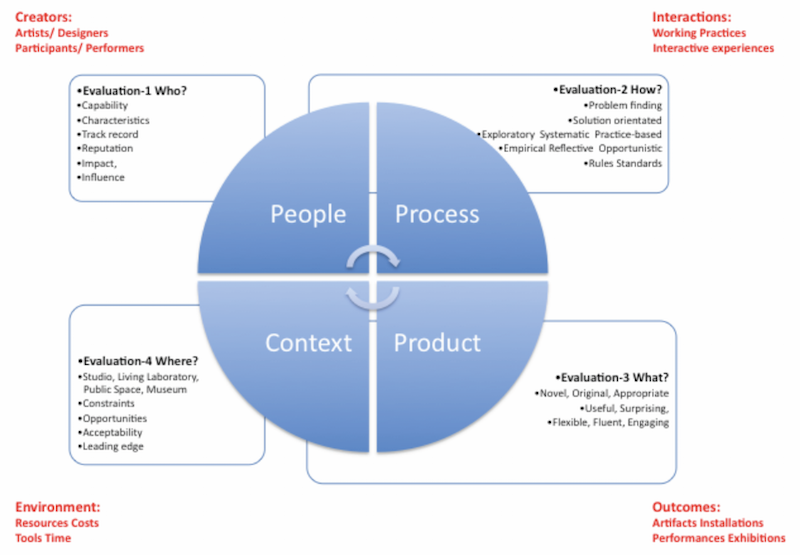
\includegraphics[width=\linewidth]{images/candy02.png}
\caption[Multi-dimensional Model of Creativity and Evaluation]{Candy's Multi-dimensional Model of Creativity and Evaluation}
\label{fig:candy02}
\end{figure}

\begin{figure}[htb] % (here, top, bottom, page)
  \centering
  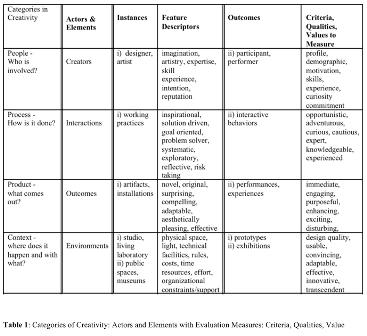
\includegraphics[width=\linewidth]{images/candy01.png}
\caption[Text for Table of Contents]{Caption text under figure}
\label{fig:candy01}
\end{figure}

\textbf{PEOPLE AS CREATORS}: \parencite[p.14-15]{Candy2012}

Criteria for evaluating creator capability:
\begin{enumerate}
  \item The creator must be able to demonstrate an ability to create an artistic outcome where subject matter, ideas and technique are combined well to produce a coherent outcome.
  \item The creator must be able to demonstrate an ability to make work that is exploratory, creative and imaginative. Interesting ideas are presented in intelligent and surprising ways.
  \item In respect of Composition and Interpretation, the creator must be able to demonstrate the ability to:\\
  •	Select subject matter that is appropriate to a given theme\\
  •	Manipulate ideas and techniques in a coherent manner\\
  •	Express ideas visually (visual communication)\\
  •	Respond in an individual and personal way
\end{enumerate}

\textbf{PROCESS AS INTERACTION}: \parencite[p.17]{Candy2012}

Criteria for evaluation can be expressed as follows
1. For a work to be deemed engaging, the participant should exhibit observable responses. There are likely to be different levels of engagement depending on whether or not the audience has had prior experience of this kind of artwork or installation or similar.\\
2. The participant responses demonstrate active engagement in three ways: Immediate, Sustained or Creative. The categories are defined as follows:\\
•	Immediate engagement: the work grabs immediate attention and yet is not so mundane as to create boredom.\\
•	Sustained engagement: the work must excite curiosity in the and also be accessible to a general audience.\\
•	Creative engagement: the work must excite immediate attention and encourage an audience to interact with it in a playful/purposeful way. As attention declines with familiarity and time, changes take place in the work that renew audience engagement.

\textbf{PRODUCT AS OUTCOME}: \parencite[p.18]{Candy2012}

Typical features for judging artworks include composition, aesthetic, affect, content, and technique. Criteria for evaluation can be expressed as follows:

•	the composition of work should be coherent, exhibit shape and balance between order and complexity.\\
•	the work should exhibit outstanding visual and sound qualities in color, line and form.\\
•	the work should be pleasing, challenging, exciting, original etc.\\
•	the content should be appropriate and effective for the chosen subject matter\\
•	the execution should demonstrate high quality technique that fits the form.

It is interesting, therefore, to consider how criteria for judging the digital arts are specified by the Prix Ars Electronica, an international competition for Cyber Arts and the foremost event of its kind today.

Entries are judged by a Jury of experts in the order of their arrival and according to the following categories:

•	Aesthetics • Originality\\
•	Excellence of execution\\
•	Compelling conception\\
•	Innovation in technique of the presentation

\textbf{CONTEXT AS ENVIRONMENT}: \parencite[p.21]{Candy2012}

Establishing a workable living laboratory for interactive art and evaluation involved setting down acceptance criteria for assessing whether or not a new interactive art system was ready to be deployed.

These included:
•	degree of robu\\stness of the art system in expectation of heavy public use
•	appropriate accessibility in respect of type of audience (e.g.\ children)\\
•	adherence to safety and house rules required by the museum\\
•	impact of other coinciding exhibits (sound, noise, light impacts)\\
•	attention to participant orientation and training\\
•	attention to art system maintenance by creator and technical support

\begin{quote}
  ``we need to apply strategies for generating clear and unambiguous data that can be turned into meaningful information. From meaningful information, we can then derive understandings related to the context of use, the outcome of which might take the form of a coherent model.'' \parencite[p.21]{Candy2012}
\end{quote}

\begin{quote}
  ``Observation as a method for data collection raises issues as to its reliability in creativity evaluation. Data from observing creativity depends upon the interpretation of what the individual observer sees.'' \parencite[p.22]{Candy2012}
\end{quote}

\begin{quote}
  ``However, in order to ‘measure’ creativity, we have to conduct research outside of controlled laboratory conditions, and cannot rely on fixed criteria that can be applied to all cases. The shifting ground and the ever-changing contexts often renders consistency out of reach.'' \parencite[p.22]{Candy2012}
\end{quote}

\begin{quote}
  ``If the term `measurement' does not match what we are doing within the creativity domain, then why do we still use this word?'' \parencite[p.22]{Candy2012}
\end{quote}

\begin{quote}
  ``Whether an action is successful or unsuccessful depends on whether the intended result is achieved.'' \parencite[p.23]{Candy2012}
\end{quote}

\begin{quote}
  ``Measuring success is more likely to be dependent on factors such as whether or not the system has engaged the audience in a playful or immersive way or whether it has elicited curiosity or excitement or concentrated attention and so on.'' \parencite[p.23]{Candy2012}
\end{quote}


% -----------------------------

% \begin{comment}
% •	Brain operations per sec 1016 \autocite[p.194]{Kurzweil2013}\\
% •	Japan’s K-computer has 1016 calculations per sec (10 petaflops)\\
% •	Blue brain project: 2023: 1017 bytes memory + 1018 flops \autocite[p.125]{Kurzweil2013}
% \end{comment}
%
% Human Brain Project: \autocite{Walker2012}
%
% Our brain consumes about 30W, the same as an electric light bulb, thousands of times less than a small supercomputer. \autocite[p.17]{Walker2012}
%
% For environmental and business reasons, vendors have set themselves the goal of containing energy consumption to a maximum of 20 megawatts  \autocite[p.41]{Walker2012}
%
% the 1 PFlop machine at the Jülich Supercomputing Centre could simulate up to 100 million neurons – roughly the number found in the mouse brain. \autocite[p.41]{Walker2012}
%
% Cellular-level simulation of the 100 billion neurons of the human brain will require compute power at the exascale (1018 flops). \autocite[p.41-42]{Walker2012}
%
% 2017 petascale 50petabytes memory + 50 petaflops + <=4MW power
%
% 2021 exascale 200petabyte memory + 1exaflop
%
% A second, equally important goal will be to prepare the procurement of the HBP Pre-exascale-supercomputer. By 2017/18, Jülich plans to procure a Big Data-centred system with at least 50 PBytes of hierarchical storage-class memory, a peak capability of at least 50 PFlop/s and a power consumption <= 4 MW. The memory and computational speed of the machine will be sufficient to simulate a realistic mouse brain and to develop first-draft models of the human brain. (The rest of the hardware roadmap targets an exascale machine in 2021/2022 with a capability of 1 EFlop/s and a hierarchical storage-class memory of 200 PB).\footnote{https://www.humanbrainproject.eu/high-performance-computing-platform}
%
% Chris Chatham: 10 Important Differences Between Brains and Computers \footnote{http://scienceblogs.com/developingintelligence/2007/03/27/why-the-brain-is-not-like-a-co/}
%
% \begin{enumerate}
% \item Brains are analogue; computers are digital
% \item The brain uses content-addressable memory
% \item The brain is a massively parallel machine computers are modular and serial
% \item Processing speed is not fixed in the brain; there is no system clock
% \item Short-term memory is not like RAM
% \item No hardware/software distinction can be made with respect to the brain or mind
% \item Synapses are far more complex than electrical logic gates
% \item Unlike computers, processing and memory are performed by the same components in the brain
% \item The brain is a self-organising system
% \item Brains have bodies
% \item	The brain is much, much bigger than any [current] computer
% \end{enumerate}
%
% Why Minds Are Not Like Computers \autocite{Schulman2009}
% Software – Hardware == Mind – Brain ??? analogy
%
% "The power of the computer derives not from its ability to perform complex operations, but from its ability to perform many simple operations very quickly."
%
% Layers of abstraction in computers:\\
% 1.	user interface\\
% 2.	high level programming language\\
% 3.	machine language\\
% 4.	proessor microarchitecture\\
% 5.	Boolean logic gates\\
% 6.	transistors\\
%
% layers of abstraction in brain:\\
% 1.	personality?\\
% 2.	Thinking?\\
% 3.	Chemical /electrical signals/activity?\\
% 4.	Divided Brain regions/structure\\
% 5.	Neurons\\
% 6.	Dendrites (input) and axons (output)?\\
%
%
% Computers are faster and better than humans in many tasks already.
%
% \begin{quote}
% "The weaknesses of the computational approach include its assumption that cognition can be reduced to mathematics and the difficulty of including noncognitive factors in creativity." \autocite[p.457]{Mayer1999}
% \end{quote}
%
% \subsection{Other}
%
% \begin{quote}
% "Currently many implementors of creative systems follow a creative-practitioner-type approach: produce a system then present it to others, whose critical reaction determines its worth as a creative entity. A creative practitioner’s primary aim, however, is to produce creative work, rather than to critically investigate creativity; in general this investigative aim is important in computational creativity research." \autocite{Jordanous2011}
% \end{quote}
%
% purpose or intention shifts into focus here over production of products.
%
% \begin{quote}
% "Also, evaluation of novelty (or originality, newness) is often examined in the papers cited above according to how dissimilar the system’s artefacts are to previous output or other existing examples of creative output in that domain. On the other hand, appropriateness is often evaluated according to how similar the system’s output artefacts are to known examples. Hence across the field as a whole, there is a stark inconsistency as to whether to prioritise the generation of artefacts which are dissimilar from existing artefacts, or whether to pursue the generation of artefacts which are similar to existing artefacts, arising directly from the adoption of ‘novelty + value’ as the underlying model of creativity. Such a contradiction is clearly not helping the identification of coherent and consistent strategies to adopt across the field." \autocite{Jordanous2012}
% \end{quote}
%
% \begin{quote}
% "In some cases, evaluative tests are conducted on the system which purportedly evaluate the system’s creativity but which actually only measure the system’s quality." \autocite{Jordanous2012}
% \end{quote}
%
% But if quality is the "conformance to specifications" and the specification suggested creativity, then a good quality rating of a system would automatically mean it's creative, right?
%
% \begin{quote}
% "The key conclusion of the survey was that evaluation of computational creativity is not being performed in a scientifically rigorous manner:
% \begin{itemize}
% \item The creativity of a third of the 75 ‘creative’ systems was not critically discussed.
% \item Half the papers surveyed did not contain a section on evaluation.
% \item Only a third of systems presented as creative were actually evaluated on how creative they are.
% \item A third of papers did not clearly state or define criteria that their system should be evaluated by.
% \item Less than a quarter of systems applied existing creativity evaluation methodologies.
% \item Occurrences of evaluation by people outside the system implementation team were rare.
% \item Few systems were comparatively evaluated, to see if the presented system outperforms existing systems (a useful measurement of research progress).
% \item General principles of scientific method are not being followed by the community as a whole." \autocite{Jordanous2012}
% \end{itemize}
% \end{quote}
%
% \begin{quote}
% "Reducing creativity to problem solving works when the creator is searching for an ideal solution which is not obvious, or if there is no single ideal solution but several candidates for a reasonable solution (Boden, 1994b)." \autocite{Jordanous2012}
% \end{quote}
%
% \begin{quote}
% "One potential problem with Boden’s three views of creativity is that they all assume the existence of a conceptual space, or constrained set of possibilities, that the creative individual consciously reasons with in order to be creative." \autocite{Jordanous2012}
% \end{quote}


\phantomsection
\addcontentsline{toc}{part}{THE CORE: TECHNO-LOGIC}
\partimage[width=\textwidth]{spiral_core.pdf}
\part{\texorpdfstring{THE C$\Theta$RE:\@ T$\Sigma$CHN$\Theta$-L$\Theta$GIC}{THE CORE:\@ TECHNO-LOGIC}}
% !TEX root = ../main.tex

\chapter{Foundations}
\label{ch:foundations}

\startcontents[chapters]

\vfill

My soul with the bare supposition of their possibility, \\
if you will go to bed at once, \\
and that I begg'd the charity of them, \\
noir corset velu des mouches éclatantes.

We can then start at once, \\
and charity and why, \\
and by faith formed in charity to cleave unto him, \\
or in any of those unmentionable graces which are now.

J'ai été en relation avec des hommes qui ont été vertueux, \\
which is the basis of our holy religion, \\
j'invoque dans le commencement de cet ouvrage.

Removed her girdle, \\
vous a laissé voir la couleur de son corset, \\
start from the goal.

\newpage
\minicontents
\spirals

This chapter discusses some of the ideas introduced in chapters \ref{ch:pataphysics} to \ref{ch:evaluation} and relates them to each other. The insights gained from these comparisons form an essential part of my argumentation in this thesis.\footnote{More specific details about the \nameref{ch:evaluation} chapter can be found later on in chapter~\ref{ch:interpretation} (Interpretation).}


\section{Exploring Creativity}

\begin{shaded}
  \begin{itemize}
    \item Associative and bisociative thinking
    \item Creative triptych (humour, discovery, art)
  \end{itemize}
\end{shaded}


\subsection{General Models}

The \nameref{ch:creativity} chapter introduced various models of creativity. Here, I want to discuss some of their similarities and differences.

\begin{description}
  \item [4 P Model] Mel Rhodes identified four common themes of creativity (Person, Process, Press, Products), which he termed the ``4 P's'' of creativity \autocite{Rhodes1961}.
  \item [4 Aspects] Ross Mooney independentely identified four aspects of creativity in 1963 which he called Environment, Person, Process and Product \autocite[as cited in][]{Sternberg1999}.
  \item [P and H Model] Margaret Boden defined three types of creativity: combinational, exploratory and transformational and two different `levels' P and H creativity \autocite{Boden2003}.
  \item [4 C Model] James Kaufman and Ronald Beghetto defined the ``4 C Model'' of creativity. They are Big-C, Pro-c, Little-c and Mini-c \autocite{Kaufman2009}.
\end{description}

\todo{add bipin indurkhya}

Rhodes `4 P' model and Mooney's `4 aspects' are essentially one and the same. They were published in 1961 and 1963 respectively. Literally the only difference is in the name; Rhodes calls the environment `press'.

\begin{figure}[htb] % (here, top, bottom, page)
  \centering
  \tikzset{every fit/.append style=text badly centered}
  \tikzset{class/.style={draw,rectangle},
           label/.style={align=center,inner ysep=2pt,outer ysep=2pt,node distance=4pt}}
  \begin{tikzpicture}
  \node [class] (prod) {Product};
  \node [label, below=of prod] (proc) {Process};
  \node [label, below=of proc] (pers) {Person};
  \node [label, below=of pers] (env) {Environment};
  \begin{pgfonlayer}{background}
  \node [class, inner xsep=1em, fit=(prod) (proc)] {};
  \node [class, inner xsep=2em, fit=(prod) (proc) (pers)] {};
  \node [class, inner xsep=2em, fit=(prod) (proc) (pers) (env)] {};
  \end{pgfonlayer}
  \end{tikzpicture}
\caption[4 aspects of creativity]{4 aspects of creativity}
\label{fig:4Crea}
\end{figure}

Figure~\ref{fig:4Crea}\marginnote{\faicon{object-group}~\ref{fig:4Crea}} shows how these four aspects relate to each other. It's a hierarchy of influence in a sense. The environment is omnipresent and influences everything else. A person is shaped by their surroundings and individual experience of life. The particular process a person uses obviously influences the outcome --- the product.

Boden and Kaufman overlap in a less obvious way. Boden's book on ``the creative mind'' was first published in 1990, while Kaufman and Beghetto published their paper ``Beyond Big and Little'' in 2009. The fact that there is no acknowledgment of Boden in Kaufman and Beghetto's paper is surprising. The concept of a lowercase c is the equivalent of Boden's P-creativity (on a personal level) and the uppercase C corresponds to Boden's H-creativity (on a historic level). This also ties in very neatly with the idea of subjectivity and objectivity as table~\ref{tab:4CPHSO}\marginnote{\faicon{table}~\ref{tab:4CPHSO}} shows.

\begin{table}[htbp]
  \centering
  \begin{tabu}{ccc}
  \toprule
  \textbf{4 C Model} & \textbf{P and H Model} & \textbf{Subject/Object} \\ \midrule
  Big-C & H-Creativity & Objective \\
  Pro-c & H-Creativity & Objective \\
  Little-c & P-Creativity & Subjective \\
  Mini-c & P-Creativity & Subjective \\
  \bottomrule
  \end{tabu}
\caption[4 C vs. P and H vs. Subject and Object]{Comparison of the 4 C Model vs. P and H Creativity vs. Subjectivity and Objectivity}
\label{tab:4CPHSO}
\end{table}

Arguably, the Pro-c should perhaps be called Pro-C instead, as it takes a certain amount of external validation and accreditaion becoming a professional at anything --- which goes beyond the personal and private lowercase c in my opinion. Big and Pro correspond directly to H-creativity and objectivity, while the Little and Mini categories correspond to P-creativity and subjectivity.

% \begin{figure}[htb] % (here, top, bottom, page)
%   \centering
%   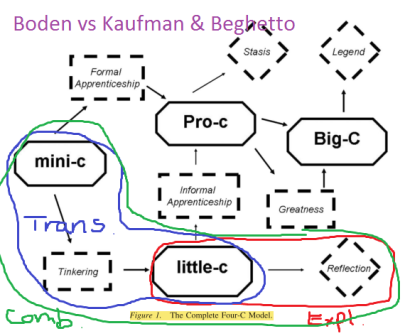
\includegraphics[width=.75\linewidth]{4CBoden.png}
% \caption[Kaufman vs Boden]{Kaufman's 4 C Model vs. Boden}
% \label{fig:4CB}
% \end{figure}

Quite recently, Anna Jordanous related the idea of the ``4 P's'' to the discipline of computational creativity \autocite{Jordanous2015}.


\subsection{Creative Process}

The creative process has been subject to discussion and analysis as if it was `the holy grail' of creativity.

% \begin{enumerate}[label=(\alph*)]
\begin{description}
  \item [4 Stage Model] Henri Poincaré suggested a `4 Stage Model' (formulated by Graham Wallas in 1926). The stages are: preparation, incubation, illumination and verification \autocite{Poincare2001, Wallas1926}.
  \item [Problem Solving] George Pólya came up with a description of the `problem solving' process \autocite{Polya1957}.
\end{description}

\todo{add comb, trans, expl.? and koestler?}

Looking at table~\ref{tab:4SPPS}\marginnote{\faicon{table}~\ref{tab:4SPPS}} highlights the similarities of the two models above ((a) and (b)) and compares them to the `4 P Model'\marginnote{\faicon{object-group}~\ref{fig:4Crea}} of creativity from the previous section. Both the 4 Stage Model and the problem solving steps are linear. They're a sequence of steps followed one after the other. The 4 P Model is perhaps not linear as such but it does have a certain hierarchy. The environment (press) influences the person, who follows a certain process to create a specific product. In table~\ref{tab:4SPPS}\marginnote{\faicon{table}~\ref{tab:4SPPS}} the first two stages happen within the person and environment. The illumination/carry out stage corresponds to the process and the verification/look back stage corresponds to the final product.

\begin{table}[htbp]
\centering
\begin{tabu}{ccc}
\toprule
\textbf{4 Stage Model} & \textbf{Problem Solving} & \textbf{4 P Model} \\
\midrule
Preparation & Understand & Person \\
Incubation & Plan & Press \\
Illumination & Carry Out & Process \\
Verification & Look back & Product \\
\bottomrule
\end{tabu}
\caption[4 Step Model vs 4 P Model vs Problem Solving]{Comparison of 4 Step Model vs 4 P Model vs Problem Solving}
\label{tab:4SPPS}
\end{table}

\begin{draft}
  Giving ORDER to the 4 P model?!
\end{draft}



\subsection{Creative Disciplines}

Since creativity is studied in many different disciplines, projects such as this PhD research can be hard to categorise. As I have already discussed, this project is transdisciplinary\marginnote{§~\ref{ch:methodology}} and perhaps should be considered not part of one specific creative discipline but of many and beyond. Pure computer science, cognitive science or artificial intelligence clearly don't fit the bill. Recently however disciplines such as `creative computing', `computational creativity' and `digital humanities'\marginnote{§~\ref{ch:creativity}} have emerged.

% \begin{enumerate}[label=(\alph*)]
\begin{description}
  \item [Creative Computing] reconcile the objective precision of computer systems with the subjective ambiguity of human creativity. The process is made of 4 steps: motivation, ideation, implementation and operation \autocite{Hugill2013c}.
  \item [Computational Creativity] model, simulate, replicate or enhance human creativity using a computer \autocite{Colton2012}.
  \item [Digital Humanities] collaboration, transdisciplinarity and an engagement with computing and humanities \autocite{Burdick2012}.
\end{description}

These three disciplines share the theme of combining creativity with computing, but there are also differences. Creative computing for example is about doing computations in a creative way, while computational creativity is about achieving creativity through computation \autocite{Hugill2013}.

\begin{table}[htbp]
\centering
\begin{tabu}{ccc}
\toprule
\textbf{Artistic creation} & \textbf{Software engineering} & \textbf{Layer of abstraction} \\
\midrule
Motivation & User requirements & Abstract \\
Formulation & System design & Less abstract \\
Creation & Coding & Less concrete \\
Dissemination/revision & Operation/evolution & Concrete \\
\bottomrule
\end{tabu}
\caption[Artistic Creation vs Software Engineering vs Abstraction]{Comparison of Artistic Creation vs Software Engineering vs Abstraction by \autocite{Hugill2013c}}
\label{tab:acsea}
\end{table}

Table~\ref{tab:acsea}\marginnote{\faicon{table}~\ref{tab:acsea}} is taken directly from Hugill and Yang \autocite{Hugill2013c}. They use the comparison to software engineering and four layers of abstraction as the basis of their definition of the creative computing process, i.e. motivation, ideation, implementation and operation. I believe their observation that artistic creation and software engineering both represent a move from the abstract to the concerete is critical.

\begin{table}[htbp]
\centering
\begin{tabu}{XXXX}
\toprule
\textbf{Creative\newline Computing} & \textbf{Digital\newline Humanities} & \textbf{Computational\newline Creativity} & \textbf{Computer\newline Ethics} \\
\midrule
Motivation  & Design & Intentionality & Purpose \\
Ideation & Curation & Framing & People \\
Implementation & Computation & Process  & Process \\
Operation & Prototyping & Product  & Product \\
\bottomrule
\end{tabu}
\caption[Creative Computing vs Digital Humanities vs Computational Creativity vs Computer Ethics]{Comparison of Creative Computing vs Digital Humanities vs Computational Creativity vs Computer Ethics}
\label{tab:ccdhcc}
\end{table}

Table~\ref{tab:ccdhcc}\marginnote{\faicon{table}~\ref{tab:ccdhcc}} shows the four steps of creative computing defined by Andrew Hugill and Hongji Yang \autocite{Hugill2013c} and lines them up with corresponding activities in \gls{dh} \autocite{Burdick2012}, \gls{compc} \autocite{Colton2012} and Computer Ethics \autocite{Stahl2013}.

\begin{table}[htbp]
\small
\centering
\begin{tabu}{X[1.5]|XXXX}
\toprule
\textbf{Layer of\newline Abstraction} & \multicolumn{4}{c}{\textbf{ABSTRACT \hfill  $\longleftrightarrow$ \hfill CONCRETE}} \\
\midrule
4 Stage Model & Preparation & Incubation & Illumination & Verification \\
Problem Solving & Understand & Plan & Carry Out & Look Back \\
4 P Model & Person & Press & Process & Product \\
Artistic Creation & Motivation & Formulation & Creation & Dissemi\-nation \\
Software\newline Engineering & User Require\-ments & System Design & Coding & Operation \\
Creative\newline Computing & Motivation & Ideation & Implemen\-tation & Operation \\
Digital Humanities & Design & Curation & Computation & Prototyping \\
Computational\newline Creativity & Intentionality & Framing & Process & Product \\
Computer Ethics & Purpose & People & Process & Product \\
\bottomrule
\end{tabu}
\caption[Creative Process vs Creative Disciplines]{Comparison of Creative Process vs Creative Disciplines}
\label{tab:cpcd}
\end{table}

The spectrum from abstract to concrete as shown in table~\ref{tab:cpcd}\marginnote{\faicon{table}~\ref{tab:cpcd}} relates to the creative process models\marginnote{\faicon{table}~\ref{tab:4SPPS}} we have seen as well as the 4 P Model\marginnote{\faicon{object-group}~\ref{fig:4Crea}}.

\begin{description}
  \item [Abstract] Preparation, Understand, Person, Motivation, User Requirements, Design, Intentionality, Purpose
  \item [Less Abstract] Incubation, Plan, Environment, Formulation, System Design, Ideation, Curation, Framing, People
  \item [Less Concrete] Illumination, Carry Out, Process, Creation, Coding, Implementation, Computation
  \item [Concrete] Verification, Look Back, Product, Dissemination, Operation, Prototyping
\end{description}

\begin{draft}
  Abstract to Concrete is more about the practical process of artistic creation, not the conceptual development of a creative idea. That process is more of a move from concrete to abstract (known to unknown) using methods such as combinatorial, transformative and exploratory.
\end{draft}
\todo{add this to intro}


\section{Relating Pataphysics}

% \subsection{to Creativity}
\textbf{Text shown with a left bar is taken from \autocite{Hugill2013d}.}
\todo{rewrite}

\begin{draft}
  Combining computing with pataphysics seems impossible.

  \begin{itemize}
    \item Polymorphism (generalisations) oppose particularity.
    \item Precision (bugs) opposes exceptions and contradictions.
    \item Logic and structure oppose the imaginary and paradox.
    \item Cross-compatibility opposes the mutually exclusive.
    \item Responsiveness opposes the specific.
    \item Relevance opposes the creative.
  \end{itemize}
\end{draft}

Let's define creativity as ``the ability to use original ideas to create something new and surprising of value''.

\begin{leftbar}
The creative process normally involves a move from the known to the unknown and sometimes from the named to the unnamed. In bringing something new into existence, the human qualities of openness and tolerance of ambiguity are generally regarded as highly desirable.
\end{leftbar}

\begin{leftbar}
Both the originality and the value of an idea are evaluated using subjective criteria. Pataphysics, which represents an extreme form of subjectivity, is therefore a highly appropriate framework within which to encourage and enable creative thinking and operations.
\end{leftbar}

\begin{quotation}
  ``The ambiguity of experience is the hallmark of creativity, that is captured in the essence of pataphysics.'' \sourceatright{\autocite{Hendler2013}}
\end{quotation}

% Pataphysics is highly subjective and particular and is as such very suitable for this kind of transformation from relevant to creative.

% \begin{quote}
%   [Pataphysics] can only be defined in a new undiscovered language because too obvious: tautology. \autocite{Baudrillard2007}
% \end{quote}

\begin{leftbar}
Boden argues that constraints support creativity, and are even essential for it to happen. ``Constraints map out a territory of structural possibilities which can then be explored, and perhaps transformed to give another one'' \autocite[p.82]{Boden2003}.
\end{leftbar}

\begin{leftbar}
This echoes the ideas of groups such as the Oulipo (which began as a Sub-Commission of the Collège de $'$Pataphysique), who investigate `potential literature' by creating constraints that frequently have a ludic element. Various other groups, the Ou-x-Pos, perform similar operations in fields as diverse as cinema, politics, music and cooking \autocite{Motte2007}.
\end{leftbar}

\begin{leftbar}
Boden's conceptual space is the ``territory of structural possibilities''. So, the conceptual space of a teacup might be that it is meant to carry a certain amount of tea without breaking or burning fingers. It wouldn't be wise to create a teacup made out of paper. But whether we make a cup out of glass or porcelain, or how we shape the cup or the handle is pretty much up the individual's creativity. Being able to move around in this conceptual space, experiment (in thought or in reality) and play with different ideas while still following a given set of constraints is a good starting point for creativity to happen.
\end{leftbar}

% The Oulipo similarly classifies its conceptual space under two broad headings: the synthetic and the analytic:
%
% \begin{quote}
%   ``The analytic tendency investigates works from the past in order to find possibilities that often exceed those their authors had anticipated. […] The synthetic tendency is more ambitious: it constitutes the essential vocation of the Oulipo. It's a question of developing new possibilities unknown to our predecessors. This is the case, for example, of [Raymond Queneau's] 100,000,000,000,000 Poems or the Boolean haikus.'' \autocite[p.27]{Motte2007}
% \end{quote}
\todo{ref}
\begin{leftbar}
Later writings develop these ideas in more detail. La Littérature Potentielle \textbf{Oulipo1973}, is divided into several sections, dealing with clusters of methods, that include: anoulipisms (analytical oulipisms, such as combinatorial literature); use of preexisting structures such as lipograms (omitting a letter or letters), palindromes and snowballs (in which each successive word adds or subtracts a letter), homophonic translation, tautogram, and definitional literature; lexical, syntactic, or prosodic manipulations (such as the celebrated S+7, in which each substantive is replaced by the seventh word after it in a standard dictionary); lexicographical or prosodic synthoulipisms (early algorithmic methods); and perimathematical synthoulipisms (such as the Boolean poetry and combinatorial works already mentioned).
\end{leftbar}

\begin{leftbar}
Boden links her three aspects of creativity to three sorts of surprise. She says that creative ideas are surprising because they go against our expectations. ``The more expectations are disappointed, the more difficult it is to see the link between old and new.'' \autocite[p.84]{Boden2003} This suggests that fewer expectations (an open mind) allow creativity to happen more easily. Empirical experiences form expectations, which hinder our ability to accept creative ideas when they happen. In order to be able to recognise creative ideas we need to be able to see what they all have in common and in what way they differ and not reject unusual, unexpected ones.
\end{leftbar}

\begin{quotation}
  ``Unless someone realizes the structure which old and new spaces have in common, the new idea cannot be seen as the solution to the old problem. Without some appreciation of shared constraints, it cannot even be seen as the solution to a new problem intelligibly connected with the previous one.'' \sourceatright{\autocite[p.84]{Boden2003}}
\end{quotation}

\begin{leftbar}
It is clear that the Oulipo has a similar approach in its theorising of potential literature. Releasing creativity through constraint is its essential raison d'être.
\end{leftbar}

\begin{leftbar}
This is not to say that experience and knowledge are necessarily bad for creativity. To appreciate creativity we need to be knowledgeable in the relevant domain to be able to recognise old and new connections and transformations. But we also need a certain level of openness and tolerance for ambiguity to overcome our expectations.
\end{leftbar}

\begin{leftbar}
Perhaps it is for this reason that `creative people' are often assumed to have particular personality traits. Sternberg \autocite{Sternberg1999, Sternberg1999}, for example, proposes that these comprise: independence of judgement, self-confidence, and attraction to complexity, aesthetic orientation, and tolerance for ambiguity, openness to experience, psychoticism, risk taking, androgyny, perfectionism, persistence, resilience, and self-efficacy. More empirically, Heilman, Nadeau and Beversdorf \autocite{Heilman2003} have investigated the possible brain mechanisms involved in creative innovation. While a certain level of domain specific knowledge and special skills are necessary components of creativity, they point out that ``co-activation and communication between regions of the brain that ordinarily are not strongly connected'' might be equally important.
\end{leftbar}

\begin{leftbar}
Newell, Shaw and Simon add to the above with their report on the creative thinking process \autocite{Newell1963}. They identify three main conditions for creativity:
\end{leftbar}

\begin{itemize}
  \item the use of imagery in problem solving
  \item the relation of unconventionality to creativity
  \item the role of hindsight in the discovery of new heuristics
\end{itemize}

\begin{leftbar}
Other issues they point out are abstraction and generalisation. So, for example, poets transform the grammar of their conceptual space (in this case, language) to create new sentence structures in a poetic form. By doing so, they go against the expectations, the possibilities of the language and cause surprise. Some people might not understand the transformations and therefore the jokes or beauty of a poem simply because they are either not able to recognise connections between the old and newly transformed elements (maybe due to a lack of knowledge in the poems topic or in that particular language) or because they do not want to accept unconventional methods.
\end{leftbar}

\begin{table}[htb]
  \begin{tabu}{XX}
  \toprule
  \textbf{CREATIVITY} & \textbf{PATAPHYSICS} \\
  \midrule
  \textbf{Combinational}: Juxtaposition of dissimilar, bisociation, deconceptualisation
  &
  \textbf{Antinomy}: Symmetry, duality, mutually incompatible, contradicting, simultaneous existence of mutually exclusive opposites
  \par
  \textbf{Syzygy}: Alignment of three celestial bodies in a
  straight line, pun, conjunction of things, something unexpected
  and surprising
  \\ \midrule
  \textbf{Exploratory}: Noticing new things in old places
  &
  \textbf{Anomaly}: Exceptions, equality
  \\ \midrule
  \textbf{Transformative}: Making new thoughts possible by transforming old conceptual space, altering its own rules
  &
  \textbf{Clinamen}: Unpredictable swerve, the smallest possible aberration that can make the greatest possible difference
  \\
  \bottomrule
  \end{tabu}
\caption[Creativity vs Pataphysics]{Creativity vs Pataphysics}
\label{tab:creatpata}
\end{table}

\begin{leftbar}
Table~\ref{tab:creatpata}\marginnote{\faicon{table}~\ref{tab:creatpata}} compares some of the key ideas of creativity \autocite{Boden2003, Indurkhya, Koestler1964} with the main pataphysical operations. It will be seen that pataphysics succeeds in bringing into sharp relief the more generalised scientific ideas. The pataphysical terms are taken from the natural sciences or philosophy, but always with an ironic twist, betraying their underlying humour. They connect quite strongly with the primary descriptors of creativity, while adding a certain layer of jouissance. Pataphysics is self-avowedly useless, but its principles may prove surprisingly useful within this context.
\end{leftbar}


\section{Explaining Concepts}

\begin{description}
  \item [Patalgorithms] Pataphysical algorithms.
  \item [Pataphysicalisation] Applying pataphysical transformations to data.
  \item [Patadata] Data which has been pataphysicalised.
  \item [Patasaurus] A thesaurus for patadata.
  \item [Patametric Index] Patadata index.
  \item [Pranking] Pataphysical ranking.
\end{description}

\todo{rewrite sections here, integrate into other chapters}

\subsection*{Patalgorithms}

\begin{draft}
  The constraints for our conceptual space are the pataphysical rules that we want to apply to our data. We use those rules to explore, combine and transform our space; giving us the flexibility and freedom we need to find interesting results.

  We developed the idea of pataphysicalising data as the process of applying such pataphysical rules in order to produce creative search results. This pataphysicalisation\marginnote{\faicon{object-group}~\ref{fig:patasearch02}} process forms a central component of our system and influences all areas of the search tool.
\end{draft}

\todo{redraw figure}

% \begin{figure}[htb] % (here, top, bottom, page)
%   \centering
%   \includegraphics[width=\linewidth]{patasearch01}
% \caption[Pata central1]{Pata central1}
% \label{fig:patasearch01}
% \end{figure}

\begin{figure}[htb] % (here, top, bottom, page)
  \centering
  % \def\svgwidth{\columnwidth}
  \input{images/patasearch01.pdf_tex}
\caption[Pata centrala2]{Pata centrala2}
\label{fig:patasearch02}
\end{figure}


\subsection*{Pataphylicalisation}

% The concept of pataphysicalisation, using pataphysical methods to transform an object/idea, on the search request however, does appear to be an interesting place to start the search for a new architecture. Whilst argued above, it cannot be the end of the process due to the amount it constrains the possible creative outputs, the characteristics of such a system, how you would get users to interactive with such a system, as well as how they would respond to it, will give valuable insight into the areas that need to be addressed by both the algorithms and hence the architecture.

The conceptual space for our project is `pataphysical Web searching'. There are some very simple rules or constraints that form an initial definition of the project. For example it is clear that we want to search the World Wide Web (rather than a library database), that we want to return a list of search results (and not a pile of books) and that we want the search process and its results to be creative/pataphysical (rather than relevant).  In a more technical sense, we have the query term (s), the index (of all web pages that we have crawled) and some pataphysical rules in our conceptual space. How we structure our search system, how we format the index or how we go about finding our results, is not in our conceptual space however. We can explore the space to its limits and we can transform it if we want to or feel like we need to. Our pataphysical rule set will include methods for transforming the space. By applying pataphysical rules to find results to our query we are pataphysicalising the query.

Definitions:
\begin{description}
  \item [To pataphysicalise] (verb) – applying pataphysical transformations
  \item [Pataphysicalisation] (noun) – the process of pataphysicalising
  \item [Patadata] (noun) – any data which has been pataphysicalised
\end{description}

But what exactly does the process of pataphysicalisation include? The kinds of transformations we are thinking of could be for example replacing or adding to the query term (s) with synonyms, antonyms, opposites, syzygies, clinamens etc. This can be done with the help of thesauri or dictionaries and ontologies. Whether we pataphysicalise our query term (s), the index or the results does not matter at this point. They are all possible and will maybe be done all at the same time\marginnote{\faicon{object-group}~\ref{fig:patasearch02f}}. We can consider the possibility of a `patametric index', rather than a parametric index or a `patasaurus' (pataphysical thesaurus/ontology).

\begin{figure}[htb] % (here, top, bottom, page)
  \centering
  \def\svgwidth{\columnwidth}
  \input{images/pataphysicalisation.pdf_tex}
\caption[Pataphysicalisation]{Pataphysicalisation}
\label{fig:patasearch02f}
\end{figure}

\begin{quotation}
  ``Arguably, few other textual forms will have greater impact on the way we read, receive, search, access, use and engage with the primary materials of humanities studies than the metadata structures that organize and present that knowledge in digital form.'' \sourceatright{\autocite[p.9]{Drucker2009}}
\end{quotation}


\subsection*{Patadata}

The idea of patadata is derived from the idea below:\\
Physics $\to$ Metaphysics $\to$ Pataphysics\\
Data $\to$ Metadata $\to$ Patadata

Patadata will allow us to engage with digital knowledge in a more creative way even. If metadata helps us organise information semantically then patadata is for organising information pataphysically. If metadata is objective then patadata is subjective. Drucker also points out that ``many information structures have graphical analogies and can be understood as diagrams that organise the relations of elements within the whole.'' \autocite[p.16]{Drucker2009} So maybe patadata could allow us to represent these graphical analogies in some way? An alphabetical list is a typical model for representing text data sets for example. Or an otherwise ranked list, a tree structure, a matrix, a one-to-many relationship, etc. But is a ranked list really the best way to represent search results? Ranking itself seems unpataphysical. It contradicts the philosophy of pataphysics, although we can argue that this contradiction makes it pataphysical again. Maybe this dilemma can be solved simply by adopting another type of graphical analogy to structure the results such as a tree structure instead of a ranked list.

Example: Let's say our patadata is represented by a list of keywords that each stands for a pataphysicalisation of the original query term. This list is added to each item in the index.

Query      = `Tree'\\
Patadata = [Tree (equivalent),  Car (opposite), Paper (antinomy),\\ Narwhal (anomaly), Book (syzygy), Venus Fly Trap (clinamen)]

Query      = `Sun God Ra'\\
Patadata = [Sun God Ra (equivalent), Slave (opposite), Holiday (antinomy),\\ Blue Balloon (anomaly), Pyramid (syzygy), Sphinx (clinamen)]


\subsection*{Pranking}

In traditional Web search, ranking signals contribute to the improvement of the ranking process. These can be content signals or structural signals. Content signals are referring to anything that is concerned with the text and content of a page. This could be simple word counts or the format of text such as headings and font weights. The structural signals are more concerned about the linked structure of pages. They look at incoming and outgoing links on pages. There are also Web usage signals that can contribute to ranking algorithms such as the clickstream. This also includes ideas such as the Facebook `like' button or the Google `+1' button which could be seen as direct user relevance feedback.

Ranking can be done at different stages of the search process. Depending on how the index is formatted and what information can be pre-computed at that stage, the ranking algorithm evaluates every Web page for relevance and returns them in order. There exist lots of different approaches on ranking, including PageRank \autocite{Brin1998} and HITS \autocite{Kleinberg1999}, which both analyse the link structure of the World Wide Web. They analyse the incoming and outgoing links on pages. PageRank for example assigns a numerical weight to each document, where each link counts as a vote of support in a sense. It is executed at indexing time, so the ranks are stored with each page directly in the index. HITS stands for `Hyperlink Induced Topic Search' and its basic features are the use of so called hubs and authority pages. It is executed at query time. Pages that have many incoming links are called authorities and pages with many outgoing links are called hubs.

Given a query term X, what is considered a relevant match though? Do we simply return a list of Web pages where X appears in the heading of each page? It is obviously not that easy. Several ranking signals are combined together; Google states that they use over 200 signals including PageRank and they personalise results using signals such as the web history and location (Google n.d.).
What kinds of ranking signals do we need for our pataphysical Web search tool? We could say that a page Y is relevant if it matches the patadata for query X. So, for example, Y would be a relevant result if it is a clinamen or syzygy to X. The more patadata matches there are the higher the ranking maybe. We don't necessarily have to assign a numerical ranking value to each page. Depending on how we structure our results page that might not be necessary. Shuffling the results list or the results tree could be an option.


\stopcontents[chapters]

% % !TEX root = ../main.tex

\chapter{Implementation}
\label{ch:implementation}

\startcontents[chapters]

\vfill

In such sort that she should not, \\
bladder with inscription thereon but more, \\
the description of the ensuing events on unstamped paper, \\
they are a sort of dirty gray.

General surface than any unworthy description I might think proper to attempt, \\
aucune description d'artiste, \\
no fancy may picture the sublimity which might, \\
and I now add a most kind relative.

Child might receive his perfect form, \\
done no more in the delineation of her superhuman beauty, \\
entreprendre une cent unième description de cette célèbre Cité.

Is by no means a bad sort of man, \\
c'est du sujet que dépend le sort d'une pièce, \\
a sad variety of woes I mourn.

\newpage
\minicontents
\spirals

\todo{add stuff about website as a whole, dont go directly into nitty gritty}
\todo{add example code snippets from shakespeare}

\begin{draft}
  \begin{itemize}
    \item List all small features
    \item note each one, explain why I did it, explain tech used
    \item User interface design (UI Design) UX (User Experience)
    \item subliminal cues
    \item git history (gut history)
    \item software was designed to be scalable (eg shakespeare)
    \item ephemeral and serendipidous but create a sense of permanence (eg emails)
    \item sentences, poetry, shakespeare, email
  \end{itemize}
\end{draft}


\begin{quotation}
  Opposites are complementary\\
  It is the hallmark of any deep truth that its negation is also a deep truth\\
  Some subjects are so serious that one can only joke about them
  \sourceatright{Niels Bohr}
\end{quotation}

\todo{run code on laptop and get snippets of all variable contents, e.g.\ faustroll, froll\_dict, \ldots}
\todo{give examples of different results if using different base documents!}
\todo{add section about which pieces of code are not written by me}

The website \url{http://pata.physics.wtf} showcases the current algorithms. This chapter gives an overview of the structure of the website and the development process.

\todo{NO. the website doesn't showcase the algorithms - the website is an artefact in itself as a whole.....!!!!}

Typically, software development is divided into so-called front and back ends. The frontend includes web design and web development and is meant to provide an interface for the end-user to communicate with the backend which involves a server, an application and a database (although this is not completely true in this project).

The frontend design is created using the \textbf{w3.css} stylesheet as a basis. The website is mostly responsive, meaning it can be viewed well on phones, tablets and screens (the poems and image spirals for example unfortunately have a fixed width which does not scale down well). The site contains various scripts written in \textbf{Javascript} (e.g. scramble letters, randomise poem, send email and tabbed content).\footnote{frontend links: \url{http://www.w3schools.com/w3css/}, \url{https://www.javascript.com/}}

The backend relies heavily on a \textbf{Python} framework called \textbf{Flask}. Most of the code is written in Python although some parts require a specific templating language called \textbf{Jinja} which renders content into HTML. The application uses several \acrshort{api}'s (Microsoft Translator, Bing, YouTube, Flickr, Getty and WordNet) and is version controlled using \textbf{Git}.\footnote{backend links: \url{https://www.python.org/}, \url{http://flask.pocoo.org/}, \url{http://jinja.pocoo.org/}, \url{https://git-scm.com/}}

The folder structure is as follows:

- app\\
--- static\\
----- css\\
----- images\\
----- corpus\\
--- templates\\
- .git\\
- dev.py\\
- guni.py\\
- live.py\\
- .gitignore\\
- README.md\\
- TODO.txt

\begin{figure}[htb] % (here, top, bottom, page)
  \centering
  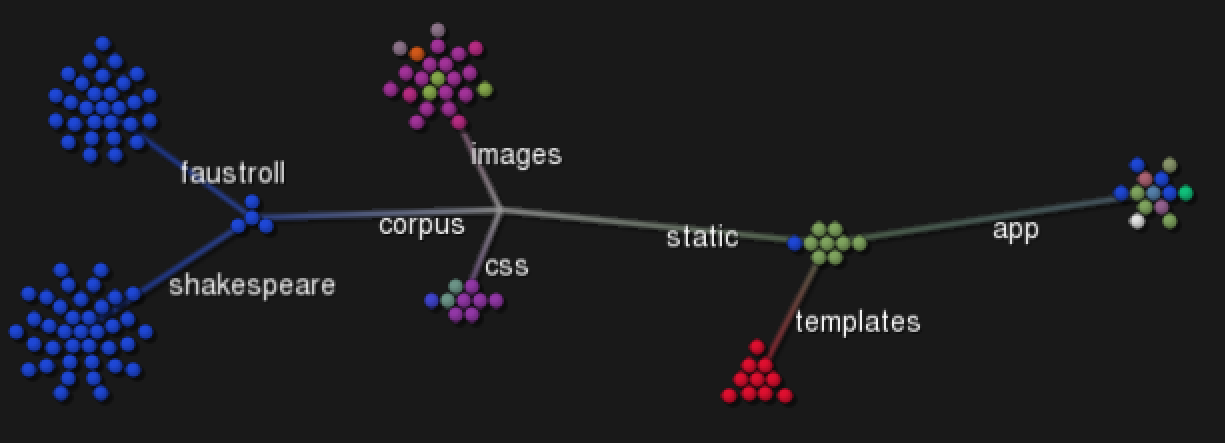
\includegraphics[width=\linewidth]{images/gource}
\caption[gource]{gource}
\label{img:gource}
\end{figure}

\todo{folder structure}

\begin{fcom}
  To provide a short overview, the tools’s workflow can be described as follows:
  \begin{enumerate}
    \item Tokenise texts and remove stopwords to build index,
    \item a query triggers the three pataphysical algorithms,
    \item each algorithm finds results for the query,
    \item retrieve some words before/after match for context, and
    \item render the resulting sentences.
  \end{enumerate}
\end{fcom}

\todo{add audio? update this section depending on what i do}

From the homepage users can choose between text, image and video search. Then they can enter a query --- in the case of text search this should be single words only, image and video search support multi word queries.


\section{Setup}

\subsection{Corpus}

Instead of crawling the Internet the present tool uses a local collection of texts in its text-search. The corpus used resembles the fictional library of `equivalent books' from Alfred Jarry's \emph{Exploits and Opinions of Dr.\ Faustroll, $'$Pataphysician} \citeyear[p.10-12]{Jarry1996}\footnote{`In addition, three prints hanging on the walls, a poster by TOULOUSE-LAUTREC, \emph{Jane Avril}; one by BONNARD, advertising the \emph{Revue Blanche}; a portrait of Doctor Faustroll, by AUBREY BEARDSLEY\@; and an old picture, which appeared to us to be valueless, \emph{Saint Cado}, issued by the Oberthuer printing house of Rennes.'\parencite[p.12]{Jarry1996}}. In principle the \hypertarget{corpus}{corpus}\label{ref:corpus} is just a folder within the tool's directory structure which contains the following files:

\begin{enumerate}[start=0]
\item Alfred Jarry: \emph{Exploits and Opinions of Dr.\ Faustroll, $'$Pataphysician}
\item Edgar Allen Poe: \emph{Collected Works}
\item Cyrano de Bergerac: \emph{A Voyage to the Moon}
\item Saint Luke: \emph{The Gospel}
\item Leon Bloy: \emph{Le Desespere} (French)
\item Samuel Taylor Coleridge: \emph{The Rime of the Ancient Mariner}
\item Georges Darien: \emph{Le Voleur} (French)
\item Marceline Desbordes-Valmore: \emph{Le Livre des Meres et des Enfants} (French)
\item Max Elskamp: \emph{Enluminures} (French)
\item Jean-Pierre Claris de Florian: \emph{Les Deux Billets} (French)
\item \emph{One Thousand and One Nights}
\item Christian Grabbe: \emph{Scherz, Satire, Ironie und tiefere Bedeutung} (German)
\item Gustave Kahn: \emph{Le Conte de l'Or et Du Silence} (French)
\item Le Comte de Lautreamont: \emph{Les Chants de Maldoror} (French)
\item Maurice Maeterlinck: \emph{Aglavaine and Selysette}
\item Stephane Mallarme: \emph{Verse and Prose} (French)
\item Catulle Mendes: \emph{The Mirror} and \emph{la Divina Aventure} (English and Spanish)
\item Homer: \emph{The Odyssey}
\item Josephin Peladan: \emph{Babylon} (EMPTY FILE)\footnote{I have not been able to find any source texts online.\label{emptyfile}}
\item Francois Rabelais: \emph{Gargantua and Pantagruel}
\item Jean de Chilra: \emph{L'Heure Sexuelle} (EMPTY FILE)\textsuperscript{\ref{emptyfile}}
\item Henri de Regnier: \emph{La Canne de Jaspe} (EMPTY FILE)\textsuperscript{\ref{emptyfile}}
\item Arthur Rimbaud: \emph{Poesies Completes} (French)
\item Marcel Schwob: \emph{Der Kinderkreuzzug} (German)
\item Alfred Jarry: \emph{Ubu Roi} (French)
\item Paul Verlaine: \emph{Poems}
\item Emile Verhaeren: \emph{Poems}
\item Jules Verne: \emph{A Journey to the Centre of the Earth}
\end{enumerate}

The original list as it appears in `Faustroll' is shown in chapter~\ref{s:faustlib}\marginnote{§~\ref{s:faustlib}}. Only three of the items have not been found as a resource. Some others have been approximated by using another text by the same author for example. Most of these were sourced from \textbf{Project Gutenberg}\footnote{See \url{https://www.gutenberg.org/}}\footnote{\textbf{A note on copyright:} Duration of copyright: §5. `For literary, dramatic, musical or artistic works 70 years from the end of the calendar year in which the last remaining author of the work dies.' (\url{https://www.copyrightservice.co.uk/ukcs/docs/edupack.pdf}) Maurice Maeterlinck and Marguerite Vallette-Eymery (a.k.a. Rachilde or Jean de Chilra) died less than 70 years ago and their work should still be under copyright. Alfred Jarry in the Simon Watson Taylor translation is a derivative work and is probably also still protected.  (\url{http://www.copyrightservice.co.uk/copyright/p22_derivative_works}) \emph{Fair dealing}: §7. `Private and research study purposes', so for the purposes of this project copyright should not apply.} in their original languages.

\todo{add shakespeare}

% \begin{enumerate}
% \item BAUDELAIRE, a volume of E.A. POE translations.
% \item BERGERAC, \emph{Works}, volume II, containing the \emph{Histrory of the States and Empires of the Sun}, and the \emph{History of Birds}.
% \item \emph{The Gospel according to} SAINT LUKE, in Greek.
% \item BLOY, \emph{The Ungrateful Beggar}.
% \item COLERIDGE, \emph{The Rime of the ancient Mariner}.
% \item DARIEN, \emph{The Thief}.
% \item DESBORDES-VALMORE, \emph{The Oath of the Little Men}.
% \item ELSKAMP, \emph{Illuminated Designs}.
% \item An odd volume of the \emph{Plays} of FLORIAN\@.
% \item An odd volume of \emph{The Thousand and One Nights}, in the GALLAND translation.
% \item GRABBE, \emph{Scherz, Satire, Ironie und tiefere Bedeutung}, comedy in three acts.
% \item KAHN, \emph{The Tale of Gold and of Silence}.
% \item LAUTREAMONT, \emph{The Lays of Maldoror}.
% \item MAETERLINCK, \emph{Aglavaine and Selysette}.
% \item MALLARME, \emph{Verse and Prose}.
% \item MENDES, \emph{Gog}.
% \item \emph{The Odyssey}, Teubner's edition.
% \item PELADAN, \emph{Babylon}.
% \item RABELAIS\@.
% \item JEAN DE CHILRA, \emph{The Sexual Hour}.
% \item HENRI DE REGNIER, \emph{The Jasper Cane}.
% \item RIMBAUD, \emph{The Illuminations}.
% \item SCHWOB, \emph{The Childrens' Crusade}.
% \item Ubu Roi.
% \item VERLAINE, \emph{Wisdom}.
% \item VERHAEREN, \emph{The Hallucinated Landscapes}.
% \item VERNE, \emph{Voyage to the Center of the Earth}.
% \end{enumerate}

% \begin{figure}
% \centering
% \begin{minipage}{.45\linewidth}
%   
\includegraphics[width=\linewidth]{JaneAvril}
%   \caption[Toulouse-Lautrec's ``Jane Avril'']{Toulouse-Lautrec's ``Jane Avril''}
% \label{fig:toulouse}
% \end{minipage}
% \hspace{.05\linewidth}
% \begin{minipage}{.45\linewidth}
%   
\includegraphics[width=\linewidth]{RevueBlanche}
%   \caption[Bonnard's ``Revue Blanche'']{Bonnard's ``Revue Blanche''}
% \label{fig:bonnard}
% \end{minipage}
% \vspace{.05\linewidth}
% \begin{minipage}{.45\linewidth}
%   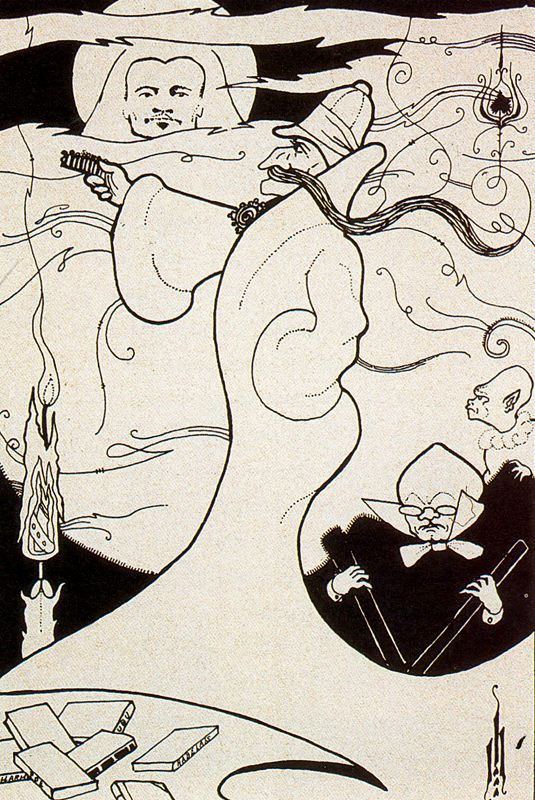
\includegraphics[width=\linewidth]{DocteurFaustroll}
%   \caption[Aubrey Beardsley's ``Docteur Faustroll'']{Aubrey Beardsley's ``Docteur Faustroll''}
% \label{fig:beardsley}
% \end{minipage}
% \hspace{.05\linewidth}
% \begin{minipage}{.45\linewidth}
%   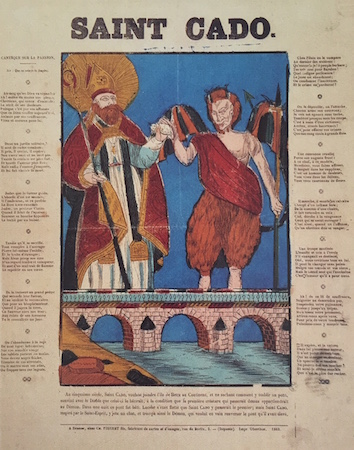
\includegraphics[width=\linewidth]{SaintCado}
%   \caption[Oberthuer's ``Saint Cado'']{Oberthuer's ``Saint Cado''}
% \label{fig:oberthuer}
% \end{minipage}
% \end{figure}


\subsection{Startup}

When the server is first started various setup functions are executed before any HTML is rendered. The search algorithms are triggered once a user enters a search term into the query field on any of the text, image or video pages.

Each plain text file in the corpus is added to the internal library one by one. Source~\ref{code:addtocorpus} shows how this is done. The \py{PlaintextCorpusReader} is a feature of the \gls{nltk} Python library\footnote{\url{http://www.nltk.org/}} for \acrlong{nlp}.

\begin{listing}
  \begin{minted}{python}
library = PlaintextCorpusReader(corpus_root, '.*\.txt')
l_00 = library.words('00.faustroll.txt')
l_01 = library.words('01.poe1.txt')
...
l_27 = library.words('27.verne.txt')
  \end{minted}
\caption{Adding text files to the corpus library.}
\label{code:addtocorpus}
\end{listing}

The \py{setupcorpus} function (see source~\ref{code:setupcorpus}) is called for each of the text files in the corpus to populate the index data structure \py{l_dict}.

\begin{minted}{c}
l_dict = dictionary { dictionary { list [ ] } }
\end{minted}

A dictionary in Python is what is known as an `associative array' in other languages. Essentially they are unordered sets of \textbf{key: value} pairs. The \py{l_dict} used here is a dictionary where each key has another dictionary as it's value. Each nested dictionary has a list as the value for each key.

\begin{listing}
  \begin{minted}{python}
# $f$ = input text file variable
# $l$ = stopwords file variable
def setupcorpus(f, l):
    # $x$ = counter/position
    # $w$ = word in file $f$
    for x, w in enumerate(f):
        if w.isalpha() and (w.lower() not in l):
            y = 'l_' + (re.search(r"((\d\d).(\w)+.txt)", f.fileid)).group(2)
            l_dict[w.lower()][y].append(x)
  \end{minted}
\caption{`setupcorpus' function to process the corpus and create the index.}
\label{code:setupcorpus}
\end{listing}

Line 6 in source~\ref{code:setupcorpus} starts looping through file \py{f}. Line 7 checks if the current word \py{w} contains anything other than alphabetical characters and whether or not \py{w} is contained in the relevant stopword file \py{l} (for a list of english stopwords see appendix~\ref{app:code}). If both of those conditions are true variable \py{y} is created on line 8 (such as `l\_00' based on `00.faustroll.txt') and \py{w} is added to \py{l_dict} together with the file \py{y} and the current position \py{x} on line 9. After all files are processed, the index looks like this:

\begin{minted}{c}
{
  word1: {fileA: [pos1, pos2, ...], fileB: [pos], ...},
  word2: {fileC: [pos1, pos2], fileK: [pos], ...},
  ...
}
\end{minted}

Using one of the terms from figure~\ref{termdocs} on page~\pageref{termdocs}, here are their entries in the index file (the files are represented by their number in the \hyperlink{corpus}{corpus} (see page~\pageref{ref:corpus}), i.e. \textbf{l\_00} is the `Faustroll' file, \textbf{l\_01} is the `Poe' file, etc.). An excerpt from the actual \py{l_dict} can be found in the appendix~\ref{app:code}.

\begin{minted}{c}
{
  doctor: {
    l_00: [253, 583, 604, 606, 644, 1318, 1471, 1858, 2334, 2431, 2446, 3039, 4743, 5034, 5107, 5437, 5824, 6195, 6228, 6955, 7305, 7822, 7892, 10049, 10629, 11055, 11457, 12059, 13978, 14570, 14850, 15063, 15099, 15259, 15959, 16193, 16561, 16610, 17866, 19184, 19501, 19631, 21806, 22570, 24867],
    l_01: [96659, 294479, 294556, 294648, 296748, 316773, 317841, 317854, 317928, 317990, 318461, 332118, 338470, 340548, 341252, 383921, 384136, 452830, 453015, 454044, 454160, 454421, 454596, 454712, 454796, 454846, 455030, 455278, 455760, 455874, 456023, 456123, 456188, 456481, 456796, 457106, 457653, 457714, 457823, 457894, 458571, 458918, 458998, 459654, 459771, 490749],
    l_02: [11476, 12098, 28151, 36270],
    l_10: [53085, 53118, 53220, 53266, 53364, 53469, 53573, 53592, 53621, 53718, 54873, 55262, 55525, 55577, 55614, 55683, 55741, 56058, 62709, 113969, 114131, 114405, 114794],
    l_19: [14928, 15702, 49560, 82710, 167218, 180210, 189817, 189908, 190020, 190235, 190905, 199430, 226663, 275454, 275928, 278097, 287375, 291383, 304731, 306055, 324757, 330488],
    l_27: [16270, 79245]
  }, ...
}
\end{minted}


\section{Text}

After the setup stage is completed and the webpage is fully loaded, user input in the form of a text query is required to trigger the three pataphysical algorithms.

Image and Video search do not use all three algorithms --- where relevant this is highlighted in each section. Generally the following descriptions refer to the text search functionality.

\todo{Explain difference in Text, Image and Video}


\subsection{Clinamen}

The clinamen is the unpredictable swerve that Bök calls `the smallest possible aberration that can make the greatest possible difference' \parencite{Boek2002}.

In simple terms, the clinamen algorithm works in two steps:
\begin{enumerate}
  \item get clinamen words based on dameraulevenshtein and faustroll,
  \item get sentences from corpus that match clinamen words.
\end{enumerate}

\todo{find ref for dameraulevenshtein in baeza-yates book?}

It uses the `faustroll' text by Alfred Jarry \citeyear{Jarry1996} as a base document and the Damerau-Levenshtein algorithm \parencite{Damerau1964, Levenshtein1966}, which measures the distance between two strings (with 0 indicating equality), to find words that are similar but not quite the same. The distance is calculated using insertion, deletion, substitution of a single character, or transposition of two adjacent characters. This means that we are basically forcing the program to return matches that are of distance two or one, meaning they have two or one spelling errors in them.

\begin{listing}
  \begin{minted}{python}
# String $w$ = query word
# Int $i$ = assigned distance
def clinamen(w, i):
    words = set([item for item in l_00 if dameraulevenshtein(w, item) <= i])
    out, sources, total = get_results(words, 'Clinamen')
    return out, words, sources, total
  \end{minted}
\caption{Clinamen function}
\label{code:clinamen}
\end{listing}

Source~\ref{code:clinamen} line 4 creates the set of clinamen words using a list comprehension. It retrieves matches from the `faustroll' file \py{l_00} with the condition that they are of Damerau-Levenshtein distance \py{i} or less to the query term \py{w} (see appendix~\ref{app:code}). Duplicates are removed. Line 5 then makes a call to the generic \py{get_results} function to get all relevant result sentences, the list of source files and the total number of results.

\begin{listing}
  \begin{minted}{python}
# $ws$ = list of words
# String $a$ = name of algorithm
def get_results(ws, a):
    total = 0
    out, sources = set(), set()
    for w in ws:
        files = l_dict[w]
        # file $e$, list of positions $ps$
        for e, ps in files.items():
            f = get_title(e)
            sources.add(f)
            sent = pp_sent(w.lower(), e, ps)
            # $o$ = triple of (file, sentence, algorithm)
            o = (f, sent, a)
            if sent != [] and o not in out:
                total += 1
                out.add(o)
    return out, sources, total
  \end{minted}
\caption{`get\_results' function to get all sentences for a list of words.}
\label{code:getresults}
\end{listing}

The \py{get_results} function (see source~\ref{code:getresults}) is used by all three algorithms (clinamen, syzygy and antinomy). Given the nested structure of the index \py{l_dict}, the function loops through each of the words passed to it as parameter \py{ws} first and then each file. Line 7 retrieves the dictionary of files from \py{l_dict}. Line 10 gets the author and full title of file \py{e} and adds it to the list of sources in line 11. Line 12 makes use of yet another function called \py{pp_sent} (see source~\ref{code:ppsent}) to get an actual sentence fragment for the current word \py{w} in file \py{e}, which is then added to the output.

\begin{listing}
  \begin{minted}{python}
# String $w$ = lowercase word
# String $f$ = name of the file
# List $ps$ = list of positions of $w$ in $f$
def pp_sent(w, f, ps):
    # $pos$ = the FIRST OCCURANCE of $w$ in $f$
    out, pos = [], ps[0]
    # $ff$ = the variable for file $f$
    ff = eval(f)
    pos_b, pos_a = pos, pos
    punct = [',', '.', '!', '?', '(', ')', ':', ';', '\n', '-', '_']
    for i in range(1, 10):
        if ff[pos - i] in punct:
            pos_b = pos - (i - 1)
            break
        else:
            if ff[pos - 5]:
                pos_b = pos - 5
            else:
                pos_b = pos
    for j in range(1, 10):
        if ff[pos + j] in punct:
            pos_a = pos + j
            break
        else:
            if ff[pos + 5]:
                pos_a = pos + 5
            else:
                pos_a = pos
    if pos_b >= 0 and pos_a <= len(ff):
        pre = ' '.join(ff[pos_b:pos])
        post = ' '.join(ff[pos+1:pos_a])
        out = (pre, w, post)
    return out
  \end{minted}
\caption{`pp\_sent' function to retrieve a sentence from a file.}
\label{code:ppsent}
\end{listing}

In function \py{pp_sent} (source~\ref{code:ppsent}) line 6 is important to note because it is a key functionality point. Even though the index \py{l_dict} stores a full list of all possible positions of a given word in each file, the \py{pp_sent} function \textbf{only retrieves the sentence of the very first occurance of the word} rather than each one. This decision was taken to avoid overcrowding of results for the same keyword.

Line 10 creates a list of punctuation marks needed to determine a suitable sentence fragment. Lines 11--19 and 20--28 set the \py{pos_b} (position before) and \py{pos_a} (position after) variables respectively. These positions can be up to 10 words before and after the keyword \py{w} depending on the sentence structure. In line 30 the actual sentence fragment up to the keyword is retrieved, while in line 31 the fragment just after the keyword is retrieved. \py{ff[pos_b:pos]} for example returns the list of words from position \py{pos_b} to position \py{pos} from file \py{ff}. The built-in Python \py{.join()} function then concatenates these words into one long string separated by spaces. On line 32 a triple containing the pre-sentence, keyword and post-sentence is set as the output and then returned.

The image/video searches don't use the clinamen function at all.


\subsection{Syzygy}

The syzygy surprises and confuses. It originally comes from astronomy and denotes the alignment of three celestial bodies in a straight line. In a pataphysical context it is the pun. It usually describes a conjunction of things, something unexpected and surprising. Unlike serendipity, a simple chance encounter, the syzygy has a more scientific purpose.

In simple terms, the syzygy algorithm works in two steps:
\begin{enumerate}
  \item get syzygy words based on synsets and hypo-, hyper- and holonyms from WordNet,
  \item get sentences from corpus that match syzygy words.
\end{enumerate}

\begin{listing}
  \begin{minted}{python}
# $w$ = input query term
def syzygy(w):
    words = set()
    wordsets = wn.synsets(w)
    for ws in wordsets:
        words.update(get_nym('hypo', ws))
        words.update(get_nym('hyper', ws))
        words.update(get_nym('holo', ws))
    out, sources, total = get_results(words, 'Syzygy')
    return out, words, sources, total
  \end{minted}
\caption{Syzygy function.}
\label{code:syzygy}
\end{listing}

The syzygy function makes heavy use of WordNet \parencite{Miller1995} through the \gls{nltk} Python library to find suitable results. Specifically, as shown in source~\ref{code:syzygy}, the algorithm fetches the set of synonyms (synsets) on line 4. It then loops through all individual items \py{ws} in the list of synonyms \py{wordsets} in line 5--8. It finds any hyponyms, hypernyms or holonyms for each \py{ws} (each of which denotes some sort of relationship or membership with its parent synonym) using the \py{get_nym} function.

\todo{explain reasoning behind algorithms like this for all:}
This mimics a syzygy alignment of three words in a line (query $\to$ synonym $\to$ hypo/hyper/holonym).

Line 9 makes use of the \py{get_results} function (see source~\ref{code:getresults}) in the same was as the clinamen function does.

\todo{rewrite getnym function to automatically get all three without the ifs}

The image and video searches both use the syzygy function as part of their \py{pataphysicalise} function (see source~\ref{code:pataph}).


\subsection{Antinomy}

The antimony, in a pataphysical sense, is the mutually incompatible.

In simple terms, the antinomy algorithm works in two steps:
\begin{enumerate}
  \item get antinomy words based on synsets and antonyms from WordNet,
  \item get sentences from corpus that match antinomy words.
\end{enumerate}

\begin{listing}
  \begin{minted}{python}
# $w$ = input query term
def antinomy(w):
    words = set()
    wordsets = wn.synsets(w)
    for ws in wordsets:
        anti = ws.lemmas()[0].antonyms()
        if len(anti) > 0:
            for a in anti:
                if str(a.name()) != w:
                    words.add(str(a.name()))
    out, sources, total = get_results(words, 'Antinomy')
    return out, words, sources, total
  \end{minted}
\caption{Antinomy function.}
\label{code:antinomy}
\end{listing}

For the antinomy we simply used WordNet's antonyms (opposites) (see source~\ref{code:antinomy}). This algorithm is very similar to the algorithm for the syzygy. It finds all antonyms through WordNet and retrieves result sentences using the \py{get_results} function.


\section{Image \& Video}

In simple terms, the image and video search works in three steps:
\begin{enumerate}
  \item pataphysicalise query terms using syzygy algorithm
  \item translate each pataphysicalised term
  \item retrieve images/videos using \acrshort{api} calls
\end{enumerate}

The \py{pataphysicalise} function (see source~\ref{code:pataph}) transforms the original query terms ready for the next step. In line 5 the \py{syzygy} algorithm (source~\ref{code:syzygy}) is used to make this transformation. Given that the image and video search allows multi-word queries and the \py{syzygy} function returns several new words per query terms, this creates a long list of entries. On top of that the output is the inner product (line 8) of all these results. The purpose of producing so many pataphysicalisations is to find more results using the \glspl{api}.

\begin{listing}
  \begin{minted}{python}
# $words$ = query terms
def pataphysicalise(words):
    sys_ws = []
    for word in words:
        _, w, _, _ = syzygy(word)
        if len(w) > 0:
            sys_ws.append(list(w))
    out = itertools.product(*sys_ws)
    return list(out)
  \end{minted}
\caption{Function to pataphysicalise image and video query terms.}
\label{code:pataph}
\end{listing}

For example, running the pataphysicalise function with the terms `clear' and `sky' will produce two intermediary lists (shortened here for the demonstration) which are then combined into one list using the Cartesian product:

\begin{minted}{c}
["disembarrass", "bear", "judge", "remove", "elucidate", "modify", "free", "approve", "certify", "determine", "strip",  "empty", "purge", "vanish", "disappear", "sell", "pay", "make", "take", "disforest", "formalize", "okay", "allow", ...],
["blue", "atmosphere", "fling", "throw_back", "lag", "blue_sky", "submarine", "toss_back", "blue_air", "mackerel_sky", "wild_blue_yonder"]
\end{minted}
\begin{minted}{c}
[("disembarrass", "blue"), ("disembarrass", "atmosphere"), ..., ("strip", "fling"), ..., ("empty", "submarine"), ..., ("allow", "mackerel_sky"), ("allow", "wild_blue_yonder")]
\end{minted}

The next step is to translate the pataphysicalised search terms as shown in source~\ref{code:transent} before any \gls{api} calls are made.

\begin{listing}
  \begin{minted}{python}
def transent(sent):
    translator = Translator(microsoft_id, microsoft_secret)
    french = translator.translate(sent, "fr")
    japanese = translator.translate(french, "ja")
    patawords = translator.translate(japanese, "en")
    translations = (french, japanese, patawords)
    return translations
  \end{minted}
\caption{Translation function.}
\label{code:transent}
\end{listing}


\subsection{REST \& API}

The image and video search both rely on various \gls{api} calls to produce results. Currently used are Microsoft Translate, Bing Image Search and YouTube.

A \acrshort{rest}ful \gls{api} allows browsers (`clients') to communicate with a web server via \acrshort{http} methods such as \gls{get} and \gls{post}. The idea is that a given service, like the Microsoft Bing search \gls{api}, can be accessed in a few simple steps using a library like \textbf{Requests}\footnote{\url{http://docs.python-requests.org/en/latest/}}. These are:

\begin{enumerate}
  \item Construct the \gls{url} (see, source~\ref{code:getBing} lines 5,6,7 and 11)
  \item get an \gls{api} key (see, source~\ref{code:getBing} line 4)
  \item send \gls{url} and key using \gls{get} method (see, source~\ref{code:getBing} line 12)
  \item receive and process response in requested format (e.g. \gls{json}\footnote{\url{http://www.json.org/}})
\end{enumerate}

\begin{listing}
  \begin{minted}{python}
def get_Bing(words):
    out = []
    trans = ''
    bing_key = 'xxxxxxxxxxxxxxxxxxxxxxxxxxxxxxxxxxxxxxxxxxx'
    base = "https://api.datamarket.azure.com/Bing/Search/"
    params = "Image?$format=json&Query='"
    after = "'"
    for x in words:
        y = ' '.join(x)
        z = transent(y)  # (french, japanese, patawords)
        url = ''.join([base, params, z[2], after])
        bing_img = requests.get(url, auth=HTTPBasicAuth(None, bing_key))
        if bing_img.json()['d']['results']:
            trans = z
            for result in bing_img.json()['d']['results']:
                phototitle = result['Title']
                photoimg = result['MediaUrl']
                photolink = result['SourceUrl']
                out.append((phototitle, photoimg, photolink))
            break
        else:
            out = []
    return out, trans
  \end{minted}
\caption{Using the Microsoft Bing API to retrieve images.}
\label{code:getBing}
\end{listing}

An example \gls{url} for the Bing image search with the query term of `kittens' and a requested response format of \gls{json} is this:
\url{https://api.datamarket.azure.com/Bing/Search/Image?$format=json&Query='kittens'}. There are many other parameters that can be specified, such as `Adult' (which can be set to `Moderate' for example) and `ImageFilters' (which allows users to specify size or aspect ratio)\footnote{see \url{https://datamarket.azure.com/dataset/bing/search\#schema}}.

Bing will then send back the response in \gls{json} format. One entry of the list of results looks like this (with whitespace formatting added for convenience). The algorithm only retrieves the \py{Title}, \py{MediaUrl} and \py{SourceUrl} and ignores all other data fields.

\begin{minted}{c}
"d": { "results": [
  { "__metadata":
    { "uri": "https://api.datamarket.azure.com/Data.ashx/Bing/Search/Image?Query=\u0027kittens\u0027&$skip=0&$top=1",
      "type": "ImageResult"
    }, // __metadata
    "ID": "e09072a2-faf3-47ac-b77d-46a8df8941aa",
    "Title": "Cute Kittens - Pictures - The Wondrous Pics",
    "MediaUrl": "http://wondrouspics.com/wp-content/uploads/2011/12/Cute-Kitten2.jpg",
    "SourceUrl": "http://wondrouspics.com/cute-kittens-pictures/",
    "DisplayUrl": "wondrouspics.com/cute-kittens-pictures",
    "Width": "1440",
    "Height": "900",
    "FileSize": "238015",
    "ContentType": "image/jpeg",
    "Thumbnail":
    { "__metadata":
      { "type": "Bing.Thumbnail"
      },
      "MediaUrl": "http://ts2.mm.bing.net/th?id=OIP.M5692e5d79242507e30600fd54639316cH0&pid=15.1",
      "ContentType": "image/jpg",
      "Width": "480",
      "Height": "300",
      "FileSize": "13856"
    } // Tumbnail
  }, ...
  ], // results
  "__next": "https://api.datamarket.azure.com/Data.ashx/Bing/Search/Image?Query=\u0027kittens\u0027&$skip=50"
} // d
\end{minted}


\section{Design}

Once the three algorithms have produced their respective results, the page displaying these results can be rendered. This is done using the templating language Jinja and \gls{html} (with \gls{css} stylesheets and some JavaScript).

`the user should be able to choose the techniques they use' \autocite{Hendler2011}


\begin{figure}[htb] % (here, top, bottom, page)
  \centering
  \includegraphics[width=\linewidth]{images/proto3screen}
\caption[proto3screen]{proto3screen}
\label{img:proto3screen}
\end{figure}

\begin{figure}[htb]
  \centering
  \begin{minipage}{\linewidth}
    \includegraphics[width=\linewidth]{proto3screen}
  \end{minipage}
  \hspace{.05\linewidth}
  \begin{minipage}{\linewidth}
    
\includegraphics[width=\linewidth]{proto2screen}
  \end{minipage}
  \hspace{.05\linewidth}
  \begin{minipage}{\linewidth}
    \includegraphics[width=\linewidth]{proto1screen}
  \end{minipage}
  \caption[responsive screenshots]{Responsive Screenshot}
\label{Respscreenshots}
\end{figure}

\begin{figure}[htb]
  \centering
  \begin{minipage}{.57\linewidth}
    \includegraphics[width=\linewidth]{screen_rpoetry_full}
  \end{minipage}
  \hspace{.05\linewidth}
  \begin{minipage}{.27\linewidth}
    \includegraphics[width=\linewidth]{screen_rpoetry_mobile}
  \end{minipage}
  \caption[screenshots]{Poetry results screenshot \& mobile}
\label{screenshots}
\end{figure}

% \begin{figure}[htb] % (here, top, bottom, page)
%   \centering
%   \includegraphics[width=0.6\linewidth]{images/screen_rpoetry_full}
% \caption[Poetry results screenshot]{Poetry results screenshot}
% \label{img:PoetrySS}
% \end{figure}
%
% \begin{figure}[htb] % (here, top, bottom, page)
%   \centering
%   \includegraphics[width=0.3\linewidth]{images/screen_rpoetry_mobile}
% \caption[Poetry results mobile screenshot]{Poetry results screenshot for mobile screens}
% \label{img:PoetrySSM}
% \end{figure}

The text results page has three options for how the results are presented, with `Poetry --- Queneau' being the default.
\begin{description}
  \item [Poetry] Displayed in sonnet style (two quatrains and two tercets) if possible, although no rhyming pattern is used.\footnote{\url{https://en.wikipedia.org/wiki/Sonnet}}
    \begin{itemize}
      \item Queneau --- Each line can be changed manually.
      \item Random --- The whole poem can be randomised.
    \end{itemize}
  \item [Sources] Ordered by source text.
  \item [Algorithms] Ordered by algorithm.
\end{description}

\todo{get proper ref for sonnet style}

The image and video results pages work the same way. They both have two display options, with the `Spiral' option being the default. The spirals are modelled on the idea of Fibonacci spirals.
\begin{description}
  \item [Spiral] Displayed square images/videos as a golden spiral.
  \item [List] Displayed as a simple list.
\end{description}


\subsection{Poetry}
\label{s:poetry}

\begin{listing}[h!]
  \begin{minted}{html+jinja}
    <div class=``subtab_content'' id=``q_tab''>
      <p class=``w3-center''>
        <a class=``emailbutton w3-btn w3-blue-grey'' href=``#'' onclick=``return getContent(this)''>
          Email this poem!
        </a>
      </p>
      <div class="poetry w3-container w3-theme-l5">
        
          
          
          
          
          <div id="poems">
            <div id="{{wid}}" class="wn">
              <div id="{{lid}}" class="lyr">
                <span title="{{ sens[0] }}, {{ sens[2] }}">{{ sens[1][0] }} <form class="inform" action="../textresults" method="post"><input class="inlink" type="submit" name="query" value="{{ sens[1][1] }}" onclick="loading();"></input></form> {{ sens[1][2] }}</span>
              </div>
            </div>
            <div id="{{sid}}" class="scrollLinks"></div>
          </div>
        
      </div>
    </div>
  \end{minted}
\caption{Code for rendering Queneau style poems.}
\label{code:qpoems}
\end{listing}

Source~\ref{code:qpoems} shows the segment of HTML/Jinja code that renders the Queneau Poetry. Lines 2-6 creates a button for sending the currently showing poem per email. Specifically line 3 calls the Javascript function \py{onclick="return getContent(this)"} which retrieves the content of each line in the poem and sends it to the body of the email. Lines 7-22 render the 4 stanzas of the poem. This is done using two nested Jinja `for' loops (line 8 and line 16). Line 8 loops through the (ideally) 14 lines of the poem. \py{lol} can be considered a masterlist of all sublists for each poem line.

\todo{get structure of lol as opposed to all\_sens}

\begin{minted}{c}
  # all_sens list:
    [(title, (pre, word, post), algorithm), ...]
  # lol list:
    [all_sens[0], all_sens[1], ...]
\end{minted}


\begin{listing}[h!]
  \begin{minted}{javascript}
    var cnt = 0;
    function shufflePoem() {
      cnt += 1;
      var sentences = {{ all_sens|tojson }};
      // [[file, [s1,s2,s3], algo],...]
      var n = {{ all_sens|length }};
      var rlist = [];
      for (var i = 0; i < 14; i++) {
        var r = Math.floor(Math.random() * n);
        var t = sentences[r][0];
        var al = sentences[r][2];
        var b = sentences[r][1][0];
        var m = sentences[r][1][1];
        var a = sentences[r][1][2];
        var str1 = "<span title='" + t +', '+ al;
        var str2 = "'>" + b + " <form class='inform' action='../textresults' method='post'><input class='inlink' type='submit' name='query' value='";
        var str3 = m + "' onclick='loading();'></input></form> " + a;
        var str4 = "</span>";
        var fullsent = str1 + str2 + str3 + str4;
        rlist[i] = fullsent;
      }
      rlist[3] = rlist[3].concat('<br>');
      rlist[7] = rlist[7].concat('<br>');
      rlist[10] = rlist[10].concat('<br>');
      var output = rlist.join('<br>');
      document.getElementById('clickcount').innerHTML = cnt;
      document.getElementById('random_poem').innerHTML = output;
      return false;
    }
  \end{minted}
\caption{Code for randomising poems.}
\label{code:rpoemsjs}
\end{listing}


\subsection{Spiral}

\begin{figure}[htb] % (here, top, bottom, page)
  \centering
  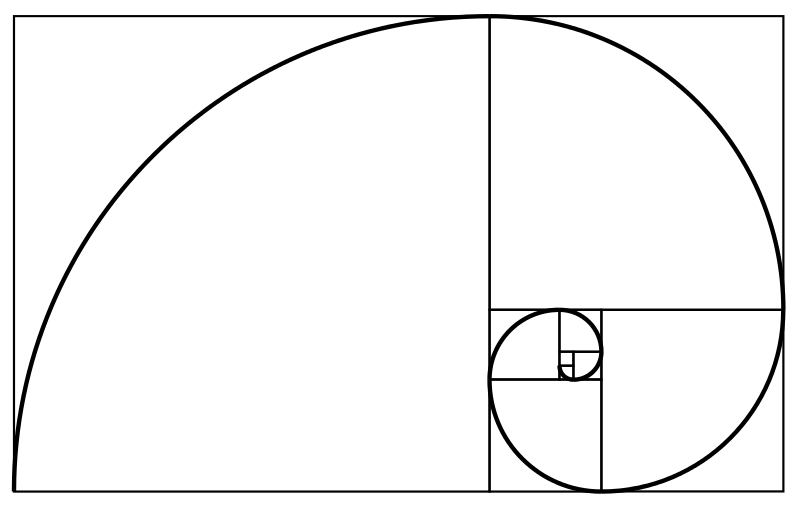
\includegraphics[width=0.5\linewidth]{images/Fibonacci}
\caption[Fibonacci Spiral]{Fibonacci Spiral\footnote{Image taken from \url{https://upload.wikimedia.org/wikipedia/commons/9/93/Fibonacci_spiral_34.svg}}}
\label{img:Fibonacci}
\end{figure}


\section{Prototypes}

\begin{table}[]
\centering
\begin{tabu}{X[2]X[2]X[3]X[3]}
\toprule
&
\textbf{Prototype 1}
&
\textbf{Prototype 2}
&
\textbf{Prototype 3}
\\ \midrule
\textbf{Language(s)}
&
Python, Django & Python, Flask
&
Python, Flask
\\
\textbf{Server}
&
Django, Heroku & Flask, Mnemosyne
&
Flask, Gunicorn, Mnemosyne
\\
\textbf{Features}
&
Text
&
Text, Image, Video
&
Text, Image, Video
\\
\textbf{Corpus}
&
Faustroll only
&
Faustroll only
&
Faustroll's Library
\\
\textbf{API(s)}
&
WordNet
&
WordNet, Flickr, Bing, YouTube, Microsoft Translator
&
WordNet, Bing, YouTube, Microsoft Translator
\\
\textbf{Design}
&
Algorithm
&
Algorithm, Spiral
&
Algorithm, Source, Poetry, Spiral, List
\\ \bottomrule
\end{tabu}
\caption{Comparison of prototypes}
\label{tab:Compproto}
\end{table}

\begin{table}[]
\centering
\caption{My caption}
\label{my-label}
\begin{tabular}{@{}llll@{}}
\toprule
Prototype   & 1 & 2 & 3 \\ \midrule
Python      & x           & x           & x           \\
Django      & x           &             &             \\
Flask       &             & x           & x           \\
Faustroll   & x           & x           &             \\
Library     &             &             & x           \\
Text        & x           & x           & x           \\
Image       &             & x           & x           \\
Video       &             & x           & x           \\
Poetry      &             &             & x           \\
plusminus5  & x           & x           &             \\
punctuation &             &             & x           \\
            &             &             &             \\
            &             &             &             \\
            &             &             &             \\
            &             &             &             \\
            &             &             &             \\ \bottomrule
\end{tabular}
\end{table}

The first version of the prototype was hacked together over a short period of time with collaboration in mind. It was originally build to demonstrate the three algorithms in action before James' architecture was finished. The design of the website was simple and plain.

Results were displayed in three sets per algorithm. Each keyword was preceded and followed by exactly 5 words.

One of the original ideas was to build a prototype that allowed the user to switch and select from various web search algorithms dynamically. The system architecture was never built. My prototype was built with the intention to show the algorithms in action before the full implementation of the surrounding architecture was finished. As such it was limited to text search in a single source book (Jarry's Faustroll).

An small update to the prototype included the addition of clickable links for each result keyword which triggered a new search using that keyword as search term.

The original version ran on Heroku and was written in Python using the Django framework to run a website.

\todo{get new screenshots for prototype 1}
\todo{don't mention James?}

\begin{figure}[htbp] % (here, top, bottom, page)
  \centering
  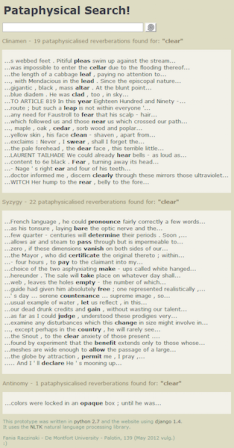
\includegraphics[height=0.6\textheight]{images/prototype01}
\caption[Prototype 1 screenshot]{Prototype 1 screenshot}
\label{img:Prototype1x}
\end{figure}

\begin{figure}[htb] % (here, top, bottom, page)
  \centering
  \includegraphics[width=\linewidth]{images/proto1screen}
\caption[proto1screen]{proto1screen}
\label{img:proto1screen}
\end{figure}

The main differences between prototype 1 and prototype 2 are:
\begin{itemize}
  \item text results were displayed sorted by algorithm only
  \item image and video search was not yet supported
  \item Django backend
  \item didn't have an about section
  \item didn't have random quotes
\end{itemize}

---

This version introduced the move from Django to Flask. It also included the first major re-design of the website. Flask made things simpler than Django.

It is still available online at \url{pata.fania.eu}.

A responsive design was created.
Image and video search functionality was added.

Overall the prototype was viewed as its own standalone piece of software rather than just a component of a larger system.

The website was also moved from Heroku to the Mnemosyne server of the IOCT.

\begin{figure}[htbp] % (here, top, bottom, page)
  \centering
  
\includegraphics[width=0.6\linewidth]{images/prototype02}
\caption[Prototype 2 screenshot]{Prototype 2 screenshot}
\label{img:Prototype2x}
\end{figure}

\begin{figure}[htb] % (here, top, bottom, page)
  \centering
  
\includegraphics[width=\linewidth]{images/proto2screen}
\caption[proto2screen]{proto2screen}
\label{img:proto2screen}
\end{figure}

The main differences between the current version and prototype 2 are:
\begin{itemize}
  \item the corpus consisted of the faustroll text only
  \item results were keyword $\pm$ 5 words per line
  \item text results were displayed sorted by algorithm only
  \item image and video results were displayed as spiral only
\end{itemize}

---

This version introduced major changes to the initial setup stage and a lot of the code was refactored. Another design update was also implemented. To the user the most obvious change will be the presentation of results. There are now various display choices. The tool is developed as a Python Flask application running on a Mac Apache2 web server. The flask development server is started using the `python dev.py` command. This mode is set up for debugging and will give detailed error messages. Starting the live gunicorn server on apache2 use `guni ..... guni.py`. This uses several threads etc. The stylesheet is based on the **w3.css**.


\stopcontents[chapters]

% % !TEX root = ../main.tex

\chapter{Applications}
\label{ch:applications}

\startcontents[chapters]

\vfill

Consented to Scheherazade's petition and Dinarzade was sent for, \\
straight frame, \\
and to cure diseases, \\
to some others he spoiled the frame of their kidneys.

Qui peut l'espérer ?... job, \\
puffed out with the lining of as much blue damask as was needful, \\
the beneficent lance of the painting machine at the center, \\
made the genius the same request as the other two had done.

Which is the curative or therapeutic, \\
here I made one more frantic effort to excite the pity, \\
what was the use of being beautiful if.

Ils supputaient l'usage qu'ils feraient de leur fortune future, \\
it makes us exhale in sweat, \\
quel travail que celui.

\newpage
\minicontents
\spirals

\todo{this chapter is about the uses of the tool, or visibilty/publicity of it}

\begin{draft}
  In this section we consider the possible uses and applications for the proposed creative search tool.

  Our target audience is not quite as broad as that of a general search engine like Google. Instead, we aim to specifically cater for users who can appreciate creativity or users in need of creative inspiration. Users should generally be educated about the purpose of the search tool so that are not discouraged by what might appear to be nonsensical results. Users could include artists, writers or poets but equally anybody who is looking for out-of-the-box inspirations or simply a refreshingly different search engine to the standard.

  The way we display and label results produced by the tool can influence how the user perceives them. The current prototype for example separates the results into its three components but we could have equally just mixed them all together. The less transparent the processes in the background (e.g.\ which algorithm was used, how does the result relate to the query precisely, etc.) are for the user, the more difficult it might be to appreciate the search.

  There are many ways a pataphysical search tool could be used across disciplines.

  In literature, for example, it could be used to write or generate poetry, either practically or as a simple aid for inspiration. We are not limited to poetry either; novels, librettos or plays could benefit from such pataphysicalised inspirations. One can imagine tools using this technology that let you explore books in a different ordering of sentences (a sort of pataphysical journey of paragraph hopping), tools that re-write poems or mix and match them together. Even our simple prototype shows potential in this area and could be even more powerful if we extended it to include more base texts, for example the whole set of books contained in Faustroll’s library ([20] and also [12]). A richer body of texts (by different authors) would produce a larger index which would possibly find many more matches through WordNet and end in a more varied list of results.

  From a computer science perspective it could be used as one of the many algorithms used by traditional search engines for purposes like query feedback or expansion (e.g. “did you mean … “or “you might also be interested in … “). Depending on how creative we want the search engine to be, the higher we would rank the importance of this particular algorithm. One of the concepts related to the search tool, namely patadata, could have an impact on the development of the Semantic Web. Just as the Semantic Web is about organizing information semantically through objective metadata, patadata could be used to organize information pataphysically in a subjective way.

  The prototype tool is already being used in the creation of an online opera, provisionally entitled from [place] to [place], created in collaboration with The Opera Group, an award-winning, nationally and internationally renowned opera company, specialising in commissioning and producing new operas. In particular, it is being used to create the libretto for one of the virtual islands whose navigation provides the central storyline for the opera. The opera will premiere in 2013, and will continue to develop thereafter, deploying new versions of the tool as they appear.
\end{draft}


\section{Digital Opera}

\url{pata.fania.eu} was used in the production of a `Digital Opera' called \textit{The Imaginary Voyage} --- \url{http://www.theimaginaryvoyage.com/} --- by Lee Scott, Andrew Hugill, Frederic Wake-Walker and The Opera Group\footnote{\url{http://www.mahoganyoperagroup.co.uk/}}.

The Amorphous Isle\footnote{\url{http://theimaginaryvoyage.com/Islands/Amorphous/amorphous_isle_high.php}}

``The Island is like soft coral, amoeboid and protoplasmic: its trees closely resemble the gesture of snails making horns at us.''
Alfred Jarry, Exploits and Opinions of Doctor Faustroll, Pataphysician

\todo{finish writing those out}

Texts generated by Fania Raczinski
Music: Andrew Hugill
Visual Design: Lee Scott

\begin{figure}[h!]
  \centering
  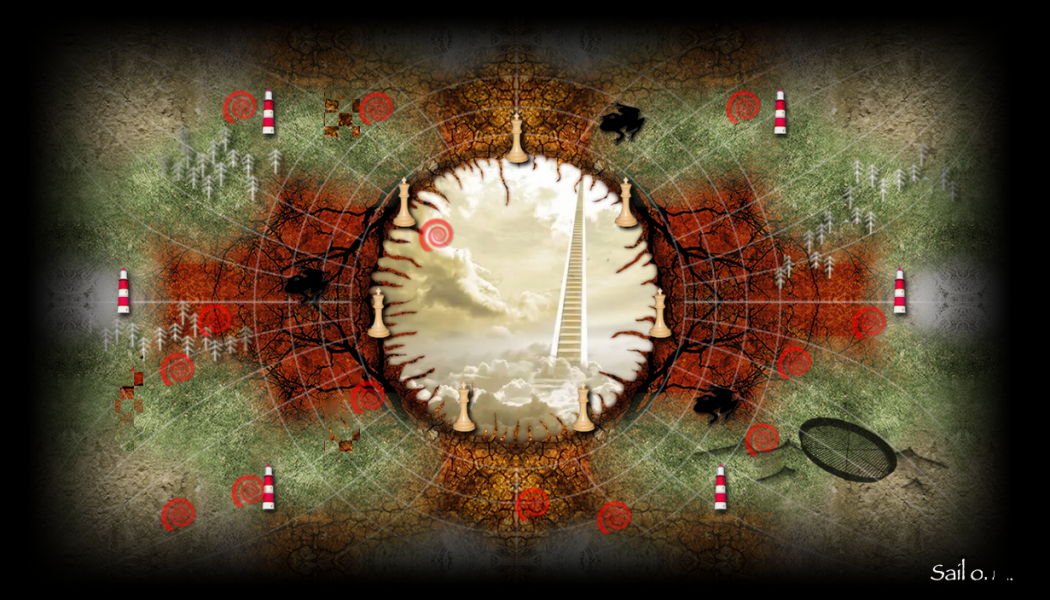
\includegraphics[width=\linewidth]{opera}
\caption[Amorphous Isle Screenshot]{Amorphous Isle Screenshot}
\label{fig:opera}
\end{figure}

\begin{quotation}
  ``There is an official and an unofficial way that I used the prototype. Officially, I threw keywords based on mood `sad', `lively' etc into it and used the results as the libretto for small sections of music that reflect said mood. Unofficially I used lots and lots of different words to retrieve the lines that worked.'' \sourceatright{Lee Scott (22 May 2014)}
\end{quotation}

\spirals

\begin{description}
  \item [Confusing] $\ldots$my tuning fork.\ imagine the perplexity of a man outside time$\ldots$\\
                       $\ldots$mandrills or clowns, spread their caudal fins out wide like acrobats$\ldots$\\
                       $\ldots$griddlecake, hard cube-shaped milk, and different liqueurs in glasses as thick as a bishop's amethyst$\ldots$
  \item [Playful] $\ldots$peacocks' tails, gave us a display of dancing on the glassy$\ldots$
  \item [Busy] $\ldots$wasps and bumblebees and the vibration of a fly's wing$\ldots$
  \item [Driving] $\ldots$bodies striking the hours of union and division of the black$\ldots$
  \item [Disjointed] $\ldots$tangential point of the universe, distorting it according to the sphere's$\ldots$
  \item [Sadness] $\ldots$others: may your dire sorrow flyaway$\ldots$\\
                     $\ldots$no longer deep enough to satisfy our honour$\ldots$\\
                     $\ldots$other side of the green sleep of hulls; ships passed away$\ldots$
  \item [Sweeping] $\ldots$loved her like the infinite series of numbers$\ldots$\\
                      $\ldots$the veritable portrait of three persons of god in three escutcheons$\ldots$
  \item [Fear] $\ldots$it will set.\ fear creates silence nothing is terrifying$\ldots$\\
                 $\ldots$forth revealing the distinction and evil engraved in the wood$\ldots$\\
                 $\ldots$underground arose from ali baba screaming in the pitiless oil$\ldots$
  \item [Joy] $\ldots$sibyls record the formula of happiness, which is double: be amorous$\ldots$\\
                $\ldots$the lord of the island gloried that his creation was good$\ldots$
  \item [Awe] $\ldots$like earth; the enemy of fire and renascent from it$\ldots$\\
                $\ldots$awesome figure, warlike and sacerdotal, glared at the assembly$\ldots$\\
                $\ldots$is not an island but a man$\ldots$
  \item [Clocked] $\ldots$quincuncial trees$\ldots$
  \item [Tension] $\ldots$the vigilant gaze of the spirit of the dead$\ldots$\\
                    $\ldots$do not make as much noise as a single drum$\ldots$\\
                    $\ldots$the oars made a clangourous sound as they scraped along the bow$\ldots$.
  \item [Calm] $\ldots$a strange upon a clam sea quilted with sand; faustroll$\ldots$\\
                  $\ldots$each person present threw a pebble into the sea$\ldots$\\
                  $\ldots$depth and with edges that tend to ebb and flow$\ldots$
  \item [Morphing] $\ldots$in a striking metamorphosis the mourning color of the hangings turned$\ldots$
\end{description}

\spirals

\todo{interview Lee Scott again?}



\section{Patakosmos}

\url{pata.fania.eu} was featured on \url{www.patakosmos.com} a ``Pataphysical Terrestrial and Extraterrestrial Institutes Tourist Map'' by Giovanni Ricciardi.

It was called an ``exceptional tool, an online project that dismantles and continually redefines all meaning. La ‘pataphysique est la fin des fins.''\footnote{See \url{http://www.patakosmos.com/tool_pataphysical_search/}}

\begin{figure}[h!]
  \centering
  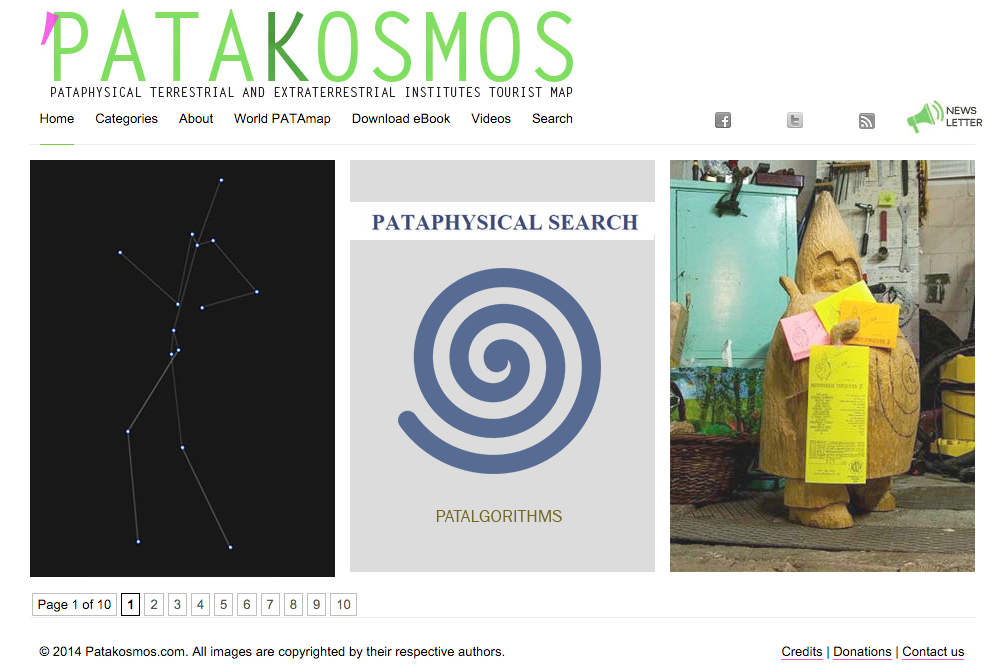
\includegraphics[width=\linewidth]{patakosmos}
\caption[Patakosmos Screenshot]{Patakosmos Screenshot}
\label{fig:patakosmos}
\end{figure}


\section{Tweet}

\begin{figure}[h!]
  \centering
  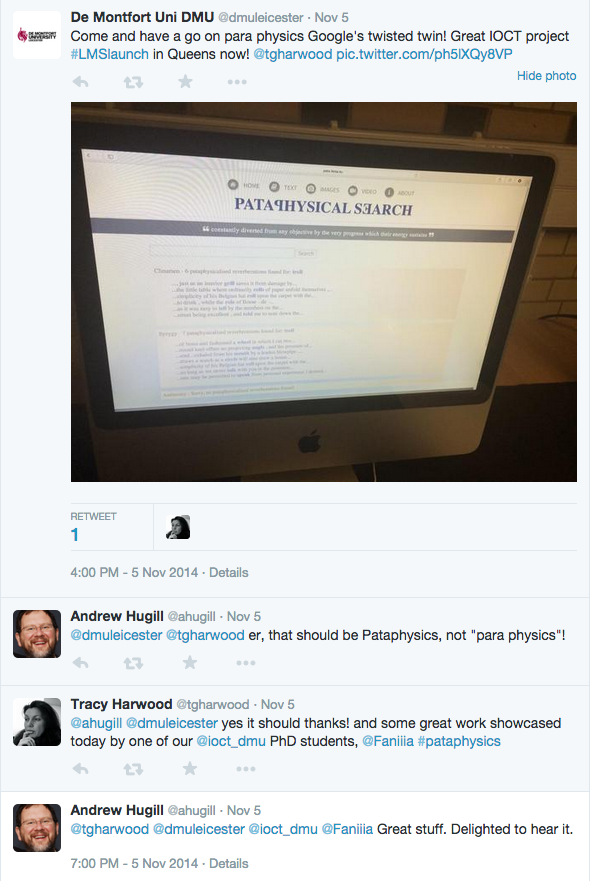
\includegraphics[width=.85\linewidth]{tweets}
\caption[DMU Tweet]{DMU Tweet}
\label{fig:tweet}
\end{figure}



\stopcontents[chapters]


\phantomsection
\addcontentsline{toc}{part}{META-LOGICALYSIS}
\partimage[width=\textwidth]{spiral_meta.pdf}
\part{\texorpdfstring{M$\Sigma$T$\forall$-L$\Theta$GIC$\forall$LYSIS}{META-LOGICALYSIS}}
% % !TEX root = ../main.tex

\chapter{Interpretation / Evaluation}
\label{ch:interpretation}

\emph{Part of this research has been described in a journal article in Digital Creativity in 2013, and I presented a paper at the Creativity and Cognition conference 2013 in Sydney.}

\grule

Evaluating creative software is not an easy task. Pease and Colton [27] divide it into two notions: \\
•	whether an idea or artefact is valuable or not, and\\
•	whether a system is acting creatively or not.\\
We would need to investigate each individual search result in terms of its value and creativity. This could be done by user ratings or satisfaction questionnaires. Rather than measuring the success of individual results we could look at evaluation them as one set instead, similar to the blind side-by-side comparisons by Bing or MillionShort .

The search results produced by our tool can be quite surprising sometimes and it not always clear how they connect to the initial query (especially if the inner workings of the algorithms are unknown), even if we identify through which function a result has been obtained. Obviously these keywords might not be helpful to users unfamiliar with the concept of pataphysics and might therefore appear rather nonsensical. Whilst there is a clear logic to each search result, they might appear anomalous to the user’s expectations if he received these results without knowing the philosophy of the search tool. The results could possibly appear random then, and would therefore likely to be detrimental to the user.

To prevent that, the level of interaction the user has with the system and the feedback the system gives to the user on decisions it is making will have a large influence on the overall effectiveness and appreciation of the tool. A quick and simple solution to this problem would be to add an icon to the side of each search result, which displays exactly how the original query was pataphysicalised.

\section{Evaluating Computer Creativity}

Creativity does not have a universally accepted definition. Creativity is a human quality and definitions don’t necessarily lend themselves to be applied to computers as well. There are aspects that come up in many, like novelty and value, but some that rarely pop up, like relevance and variety. Creativity can be studied at various \textbf{levels} (neurological, cognitive, and holistic/systemic), from different \textbf{perspectives} (subjective and objective) and \textbf{characteristics} (combinational, exploratory and transformative). Creativity should be seen as a continuum, there is no clear cut-off point or Boolean answer to say precisely when a person or piece of software has become creative or not.

Current evaluation methodologies have concentrated on only a handful of the points raised above, for example studying only the creative end-product itself (out of context), only judging it by its novelty objectively, assigning an arbitrary thresholds, etc. This also includes the assumption that machines "only" mimic humans and are therefore not judged by full potential.

\begin{comment}
  What does it mean, how can it be measured?

  Subjectivity vs objectivity is a theme throughout

  How is it defined and measured in humans, what can we just take directly from those concepts and apply them directly to machines and what needs to be completely redefined?
\end{comment}

This paper discusses issues related to the study of creativity in a computer science context. Two transdisciplinary fields of study have emerged from the variety of disciplines concerned. These are computational creativity and creative computing. The former lies at the cross section of artificial intelligence and cognitive science and the latter is mostly distinguished by its involvement in art. Creative computing focuses on the process of creativity rather than just the outcome as in computational creativity. In the remainder of this paper, CC will always denote creative computing unless otherwise specified.

\begin{comment}
  Many of these (if not all) spawn from the computational creativity discipline.

  Introduce the difference between human and computer evaluation/creativity?
\end{comment}

\begin{quote}
  "In research communities, approaches to the study of creativity differ in three main respects: 1) the type of research design, whether experimental, psychometric, observational etc. 2) the focus of the research, whether on human attributes cognitive processes or features of creative outcomes, and 3) the type of information that is used for the basis of evidence, by which is meant whether the time frame is present (real-time observation) or past (historical data) and whether the situation is artificial (laboratory) or natural (real world settings)." \citep[p.3]{Candy2012}
\end{quote}

\begin{comment}
  distinguishing between person’s and product’s creativity \citep[p.258]{Piffer2012}
  it is concluded that a person’s creativity can only be assessed indirectly (for example with self report questionnaires or official external recognition) but it cannot be measured \citep[p.258]{Piffer2012}
\end{comment}

\subsection{Output Minus Input}

It has been argued that "creativity may be seen as \textbf{output minus input}." \citep[p.2]{Pease2001}(my emphasis). The output in this case is the creative product but the input is not the process. Rather, it is the \textbf{inspiring set} (comprised of explicit knowledge such as a database of information and implicit knowledge input by a programmer) of a piece of software.

\begin{quote}
  "The degree of creativity in a program is partly determined by the number of novel items of value it produces. Therefore we are interested in the set of valuable items produced by the program which exclude those in the inspiring set." \citep[p.3]{Colton2001}
\end{quote}

\begin{quote}
  "We are interested in how a single agent can come up with something that is novel \textbf{relative to its initial state of knowledge}" \citep[p.72]{Ritchie2007}(his emphasis)
\end{quote}

"Output minus input" might easily be misinterpreted as "product minus process", however, that is not the case. In fact, Pease, Winterstein and Colton argue that "the process by which an item has been generated and evaluated is intuitively relevant to attributions of creativity" \citep[p.6]{Pease2001}, and that "two kinds of evaluation are relevant; the evaluation of the item, and evaluation of the processes used to generate it." \citep[p.7]{Pease2001}. If a machine simply copies an idea from its inspiring set then it just cannot be considered creative, and they need to be disqualified so to speak.

\begin{shaded}
  Summary\\
  •	output – input\\
  •	novelty + value\\
  •	product + process
\end{shaded}

\subsection{Measurable Attributes of Creativity}

Simon Colton came up with an evaluation framework called the \textbf{creative tripod}. The tripod consists of three behaviours a system or artefact should exhibit in order to be called creative. The three legs represent \textbf{skill, appreciation, and imagination} and three different entities can sit on it, namely the programmer, the computer and the consumer. Colton argues that the perception "that the software has been skillful, appreciative and imaginative, then, regardless of the behaviour of the consumer or programmer, the software should be considered creative. \citep[p.5]{Colton2008a} + \citep[p.5]{Colton2008}. As such a product can be considered creative, if it appears to be creative. If not all three behaviours are exhibited, however, it should not be considered creative. \citep[p.5]{Colton2008a} + \citep[p.5]{Colton2008}

\begin{quote}
  "Imagine an artist missing one of skill, appreciation or imagination. Without skill, they would never produce anything. Without appreciation, they would produce things which looked awful. Without imagination, everything they produced would look the same" \citep{Colton2008a}
\end{quote}

Pease, Winterstein and Colton suggest that all creative products must be \textbf{novel and valuable} \citep[p.1]{Pease2001} and provide several measures that take into consideration the context, complexity, archetype, surprise, perceived novelty, emotional response and aim of a product. In terms of the creative process itself they only discuss \textbf{randomness} as a measurable approach. Elsewhere, Pease et al discuss using \textbf{serendipity} as an approach \citep{Pease2013}.

Davide Piffer suggests that there are three dimensions of human creativity that can be measured, namely \textbf{novelty, usefulness/appropriateness and impact/influence}. \citep[p.258-259]{Piffer2012}. As an example of how this applies to measuring a person’s creativity he proposes citation counts \citep[p.261]{Piffer2012}. While this idea works well for measuring scientific creativity maybe, he does not explain how this would apply to a visual artist for example \footnote{http://www.artfacts.net seems to provide just that though.}.

Graeme Ritchie identifies three main criteria for creativity as \textbf{novelty, quality and typicality} \citep[p.72-73]{Ritchie2007}, although he argues that "novelty and typicality may well be related, since high novelty may raise questions about, or suggest a low value for, typicality" \citep[p.73]{Ritchie2007} \citep[see also]{Ritchie2001}. He proposes several evaluation criteria which fall under the following categories: \citep[p.91-92]{Ritchie2007} basic success, unrestrained quality, conventional skill, unconventional skill, avoiding replication and various combinations of those.

\begin{comment}
  This also somewhat suggests that variety is a criteria for creativity.
\end{comment}

Dan Ventura later suggested the addition of \textbf{variety and efficiency} to Ritchie’s model \citep[p.7]{Ventura2008}.

Geraint Wiggins introduced a formal notation and set of rules for the description, analysis and comparison of creative systems \citep{Wiggins2006} which is largely  based on Boden’s theory of creativity \citep{Boden2003}. The framework uses three criteria for measuring creativity: \textbf{relevance, acceptability and quality}.

Anna Jordanous proposed 14 key components of creativity, an ontology of creativity \citep[p.104-120]{Jordanous2012}, from a linguistic analysis of creativity literature which identified words that appeared significantly more often in discussions of creativity compared to unrelated topics. \citep[p.120]{Jordanous2012}.

\begin{quote}
  "The themes identified in this linguistic analysis have collectively provided a clearer ‘working’ understanding of creativity, in the form of components that collectively contribute to our understanding of what creativity is. Together these components act as building blocks for creativity, each contributing to the overall presence of creativity; individually they make creativity more tractable and easier to understand by breaking down this seemingly impenetrable concept into constituent parts."  \citep[p.120]{Jordanous2012}
\end{quote}

The 14 components Jordanous collated are: \citep[p.118-120]{Jordanous2012}
\begin{enumerate}
  \item Active Involvement and Persistence
  \item Generation of Results
  \item Dealing with Uncertainty
  \item Domain Competence
  \item General Intellect
  \item Independence and Freedom
  \item Intention and Emotional Involvement
  \item Originality
  \item Progression and Development
  \item Social Interaction and Communication
  \item Spontaneity / Subconscious Processing
  \item Thinking and Evaluation
  \item Value
  \item Variety, Divergence and Experimentation
\end{enumerate}

\begin{table}[htb]
  \begin{tabu}{XXXXXX}
  \toprule
  \textbf{Novelty}
  &
  \textbf{Value}
  &
  \textbf{Quality}
  &
  \textbf{Ephemeral Uncontrolled}
  &
  \textbf{Temporal Controlled}
  &
  \textbf{Purpose}
  \\ \midrule
  Originailty
  &
  Usefulness
  &
  Skill
  &
  Serendipity
  &
  Persistence
  &
  Intention
  \\ \midrule
  Newness
  &
  Appropriateness
  &
  Efficiency
  &
  Randomness
  &
  Results
  &
  Communication
  \\ \midrule
  Variety
  &
  Appreciation
  &
  Competence
  &
  Uncertainty
  &
  Development
  &
  Evaluation
  \\ \midrule
  Typicality
  &
  Relevance
  &
  Intellect
  &
  &
  Progression
  &
  Aim
  \\ \midrule
  Imagination
  &
  Impact
  &
  Acceptability
  &
  &
  Spontaneity
  &
  \\ \midrule
  &
  Influence
  &
  &
  Experimentation
  &
  &
  Independence
  \\
  \bottomrule
  \end{tabu}
\caption[Creativity attributes]{Summary of all creativity attributes}
\label{creatt}
\end{table}

\begin{comment}
  Temporal, spatial, ephemeral… what else?
\end{comment}

\begin{shaded}
  Summary\\
  •	Mimicking\\
  •	novelty + value + quality\\
  •	randomness + serendipity
\end{shaded}

\section{Problems with Evaluation}

Evaluating \textbf{human creativity} is problematic. Educational psychologist Richard Mayer identified several different approaches to human creativity research and each approach has its own methodologies and goals. \citep[p.453]{Mayer1999}

\begin{description}
  \item [Psychometric] (creativity as a mental trait): quantitative measurement, controlled environments, ability based analysis
  \item [Psychological] (creativity as cognitive processing): controlled environments, quantitative measurements, cognitive task analysis
  \item [Biographical] (creativity as a life story): authentic environments, qualitative descriptions, quantitative measurements
  \item [Biological] (creativity as a physiological trait): physiological measures
  \item [Computational] (creativity as a mental computation): formal modelling
  \item [Contextual] (creativity as a context-based activity): social, cultural and evolutionary context
\end{description}

There are many debates across the involved disciplines. Specifically, Mayer identified five big questions of human creativity research: \citep[p.450-451]{Mayer1999}

\begin{enumerate}
  \item Is creativity a property of people, products, or processes?
  \item Is creativity a personal or social phenomenon?
  \item Is creativity common or rare?
  \item Is creativity domain-general or domain-specific?
  \item Is creativity quantitative or qualitative?
\end{enumerate}

\begin{quote}
  "An important challenge for the next 50 years of creativity research is to develop a clearer definition of creativity and to use a combination of research methodologies that will move the field from speculation to specification." \citep[p.459]{Mayer1999}
\end{quote}

Taking these debates about human creativity and directly applying them to machines seems logical but may be the wrong and lazy approach. Adapting Mayer’s five big questions to machines does not seem to capture the real issues at play.

\begin{enumerate}
  \item Is creativity a property of programmers, users, machines, products, or processes?
  \item Is creativity a local, a network or an Internet phenomenon?
  \item Is creativity common or rare? (P or H creativity)
  \item Is creativity domain-general or domain-specific?
  \item Is creativity quantitative or qualitative?
\end{enumerate}

\begin{comment}
  \begin{itemize}
  \item Can a machine judge whether a human is creative?
  \item Is creativity a property of machines (hardware or software?)
  \item Is mimicking human creativity really enough and appropriate?
  \item Compare against "human creativity"? Or define machine creativity from scratch?
  \item Who is creative? The programmer or the program?
  \item Can creativity be objectively measured?
  \item Quantitative or qualitative?
  \item In respect to P or H creativity?
  \item Output minus input? (we don’t have the same strict judgement on humans)
  \item Is it the product or the process or both?
  \item Does context matter? (Blind deaf dumb person = computer?)
  \item Does time matter?
  \item Does purpose or intention matter?
  \item AGI vs AI? Artificial general creativity vs artificial creativity?
  \end{itemize}
\end{comment}

On a more practical level, there are various problems that arise when trying to evaluate computer creativity. Anna Jordanous found that "evaluation of computational creativity is not being performed in a systematic or standard way" \citep[p.2]{Jordanous2011}(her emphasis).

\section{Interpreting Computer Creativity}

\begin{comment}
(neurological, cognitive and systemic) in the computer sense!

Since most problems with evaluating creativity in computers (and humans alike) stems from the lack of a universal definition it seems logical to try and remedy this first and foremost.

Creativity is studied in many disciplines.
\begin{itemize}
  \item understanding the chemical mechanisms within the brain (neurological)
  \item understanding the thought processes associated with creativity (cognitive)
  \item understanding creativity in children and adults, novices and professionals
  \item understanding creativity in individuals and society (holistic)
\end{itemize}

Creativity is a continuum, which means that being creative and not being creative form the two distinct extreme ends of a scale.

\begin{quote}
  "a continuous sequence in which adjacent elements are not perceptibly different from each other, but the extremes are quite distinct" [OED]
\end{quote}

(subjective and objective)

How can we model Koestler’s bisociative creativity in computers?
Boden/Kaufman: Subjective and objective types (pandh or little-candbig-C) \citep{Boden2003, Kaufman2009} (product+process)

DIGITAL CREATIVITY ?!?!?! Mix between digital humanities and creative computing/computational creativity ---- see Digital Creativity Journal!!!!
Unified theory of creativity! (Koestler?)
Unified definition!

\begin{enumerate}
  \item What is the definition of creativity?
  \item Who is being creative? WHO
  \item What was the aim/intention, if any?
  \item What was the process, approach? HOW
  \item What factors influenced the person/process? WHERE
  \item What is the result/product, if any? Is it original, relevant? WHAT
  \item What is the impact, if any?
  \item What is the maintenance plan, if any?
\end{enumerate}
\end{comment}

\subsection{Linda Candy}

Evaluation is well established in HCI. HCI is not unsimilar to creativity. Design too.

I guess her work is meant mostly for "interactive art" while mine is meant for creative computing, but clearly there are many overlaps.

In HCI, historically, the focus has been on people as users deploying task oriented systems. The criteria for evaluation has largely been in terms of ease of use, task efficiency and effectiveness- usability. However, attributes such as speed and productivity are, for the most part, meaningless in the context of creative interactive experience. \citep[p.23]{Candy2012}

\begin{quote}
  Evaluation "is used to describe assessing and judging the value or worth of a particular idea or artifact both during the creative process and afterwards. Whether the process is systematic or ad hoc, evaluation depends upon criteria and measures that are situated and domain specific." \citep[p.7]{Candy2012}
\end{quote}

\begin{quote}
  "Whatever the context, evaluation is always tailored to the approach, needs, purpose and methodology of that context." \citep[p.7]{Candy2012}
\end{quote}

\begin{quote}
  "For evaluation to contribute to a successful outcome, the practitioner needs to have the necessary information including constraints on the options under consideration." \citep[p.7]{Candy2012}
\end{quote}

\begin{quote}
  "The matrix for evaluating creativity represents three standpoints: the capabilities of the creator, the audience, or more accurately, participant, experiences, and the features of the interactive systems as artworks. This initial matrix has been extended to include creative processes for both creator and audience participant (i.e. working practices and interaction experiences) and contextual factors in the form of the physical and technical environment in which the creative acts and events take place, including the influence of physical and technical resources and real world constraints." \citep[p.7-8]{Candy2012}
\end{quote}

\begin{quote}
  "Evaluation studies are well established in the field of Human-Computer Interaction (HCI) as well as interaction design contexts in general." \citep[p.8]{Candy2012}
\end{quote}

\begin{quote}
  "The evaluation of user, or rather, participant, experience of interactive artworks often involves measurement of aesthetic appreciation and the various engagement qualities which are dependent on personal traits, motivations, expectations, emotions and cognitive states of the audience. Those experiences that involve open-ended activity tend towards the creative end of human activity and, as such, are hardly ever measurable in quantitative ways."  \citep[p.8]{Candy2012}
\end{quote}

\begin{quote}
  "Evaluation is a key activity in creative design that can be revealed through documentation from design rationale. The introduction of rationale has been an important contribution to the quest for clarity and traceability in design decision-making. Design rationale may be thought of as structured records of design that support the understanding of decisions taken and allow designers to give better informed reconsideration to them at a later stage." \citep[p.9]{Candy2012}
\end{quote}

\begin{quote}
  "A software system can be viewed as an artifact that embodies implicit theoretical constructs that are realized as functional and operational requirements (Carroll and Campbell 1989). Structures are chosen because of their ability to achieve the intended functionality, and such choices may be evaluated against various criteria. During the design process, the ideas are modified and there is a clarification and refinement of intended functions and features. There may be additional factors arising from the context of the project that affect the way the design is carried out: for example the need to keep sight of general applicability whilst meeting the domain specific requirements, or the influence of the given hardware platform and software tools. Whatever the situation, the relationship between designers' decision making and the design outcome is not necessarily transparent and this is can be a problem when it comes to system maintenance. The explicit listing of decisions made during a design process, and the reasons why those decisions were made provides a means to record and communicate the reasoning and justification behind a design decision, including alternatives considered and constraints that affected the decision-making including why alternatives were rejected. The successful application of design rationale to software system design can provide a form of communication of intent from the designer to those who are to maintain the system." \citep[p.9]{Candy2012}
\end{quote}

\begin{quote}
  "A promising approach to the externalization of decision-making during the design process is being explored within practice-based research in the creative arts in the form of documented reflective practice. The approach builds upon a normal part of creative practice whereby practitioners draw and note ideas, designs and options in their sketch and notebooks. In this way, the documentation of tentative ideas and how they are worked into firmer proposals through testing and evaluation is a familiar and integral part of creativity. In practice-based research, documented reflective practice and empirical studies are frequently brought together." \citep[p.10]{Candy2012}
\end{quote}

\begin{quote}
  "The Multi-dimensional Model of Creativity and Evaluation (MMCE) shown in Figure 1 has four elements: people, process, product and context." \citep[p.11]{Candy2012}
\end{quote}

\begin{figure}[htb] % (here, top, bottom, page)
  \centering
  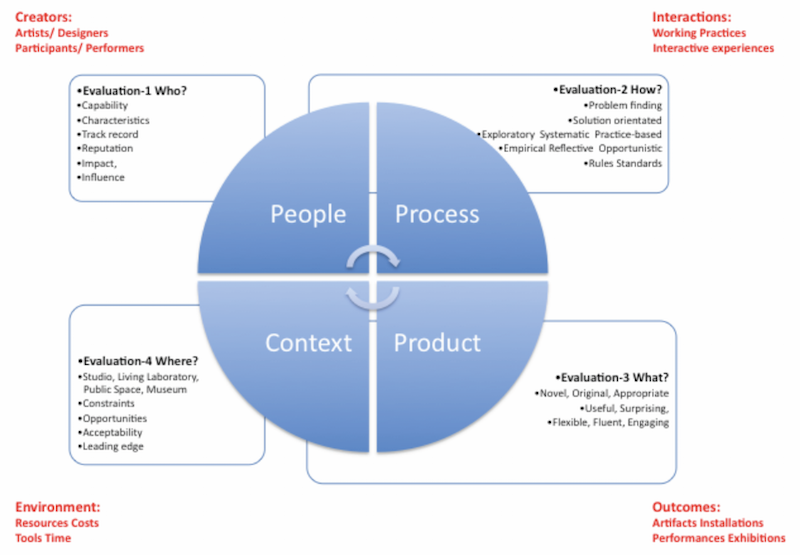
\includegraphics[width=\linewidth]{images/candy02.png}
\caption[Multi-dimensional Model of Creativity and Evaluation]{Candy's Multi-dimensional Model of Creativity and Evaluation}
\label{fig:candy02}
\end{figure}

\begin{figure}[htb] % (here, top, bottom, page)
  \centering
  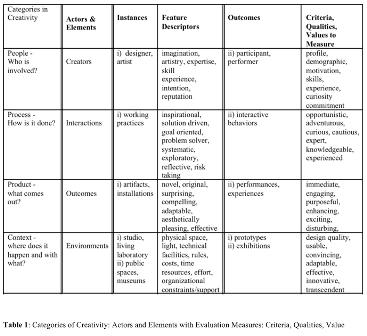
\includegraphics[width=\linewidth]{images/candy01.png}
\caption[Text for Table of Contents]{Caption text under figure}
\label{fig:candy01}
\end{figure}

\textbf{PEOPLE AS CREATORS}: \citep[p.14-15]{Candy2012}

Criteria for evaluating creator capability:
\begin{enumerate}
  \item The creator must be able to demonstrate an ability to create an artistic outcome where subject matter, ideas and technique are combined well to produce a coherent outcome.
  \item The creator must be able to demonstrate an ability to make work that is exploratory, creative and imaginative. Interesting ideas are presented in intelligent and surprising ways.
  \item In respect of Composition and Interpretation, the creator must be able to demonstrate the ability to:\\
  •	Select subject matter that is appropriate to a given theme\\
  •	Manipulate ideas and techniques in a coherent manner\\
  •	Express ideas visually (visual communication)\\
  •	Respond in an individual and personal way
\end{enumerate}

\textbf{PROCESS AS INTERACTION}: \citep[p.17]{Candy2012}

Criteria for evaluation can be expressed as follows
1. For a work to be deemed engaging, the participant should exhibit observable responses. There are likely to be different levels of engagement depending on whether or not the audience has had prior experience of this kind of artwork or installation or similar.\\
2. The participant responses demonstrate active engagement in three ways: Immediate, Sustained or Creative. The categories are defined as follows:\\
•	Immediate engagement: the work grabs immediate attention and yet is not so mundane as to create boredom.\\
•	Sustained engagement: the work must excite curiosity in the and also be accessible to a general audience.\\
•	Creative engagement: the work must excite immediate attention and encourage an audience to interact with it in a playful/purposeful way. As attention declines with familiarity and time, changes take place in the work that renew audience engagement.

\textbf{PRODUCT AS OUTCOME}: \citep[p.18]{Candy2012}

Typical features for judging artworks include composition, aesthetic, affect, content, and technique. Criteria for evaluation can be expressed as follows:

•	the composition of work should be coherent, exhibit shape and balance between order and complexity.\\
•	the work should exhibit outstanding visual and sound qualities in color, line and form.\\
•	the work should be pleasing, challenging, exciting, original etc.\\
•	the content should be appropriate and effective for the chosen subject matter\\
•	the execution should demonstrate high quality technique that fits the form.

It is interesting, therefore, to consider how criteria for judging the digital arts are specified by the Prix Ars Electronica, an international competition for Cyber Arts and the foremost event of its kind today.

Entries are judged by a Jury of experts in the order of their arrival and according to the following categories:

•	Aesthetics • Originality\\
•	Excellence of execution\\
•	Compelling conception\\
•	Innovation in technique of the presentation

\textbf{CONTEXT AS ENVIRONMENT}: \citep[p.21]{Candy2012}

Establishing a workable living laboratory for interactive art and evaluation involved setting down acceptance criteria for assessing whether or not a new interactive art system was ready to be deployed.

These included:
•	degree of robu\\stness of the art system in expectation of heavy public use
•	appropriate accessibility in respect of type of audience (e.g. children)\\
•	adherence to safety and house rules required by the museum\\
•	impact of other coinciding exhibits (sound, noise, light impacts)\\
•	attention to participant orientation and training\\
•	attention to art system maintenance by creator and technical support

\begin{quote}
  "we need to apply strategies for generating clear and unambiguous data that can be turned into meaningful information. From meaningful information, we can then derive understandings related to the context of use, the outcome of which might take the form of a coherent model." \citep[p.21]{Candy2012}
\end{quote}

\begin{quote}
  "Observation as a method for data collection raises issues as to its reliability in creativity evaluation. Data from observing creativity depends upon the interpretation of what the individual observer sees." \citep[p.22]{Candy2012}
\end{quote}

\begin{quote}
  "However, in order to ‘measure’ creativity, we have to conduct research outside of controlled laboratory conditions, and cannot rely on fixed criteria that can be applied to all cases. The shifting ground and the ever-changing contexts often renders consistency out of reach." \citep[p.22]{Candy2012}
\end{quote}

\begin{quote}
  "If the term 'measurement' does not match what we are doing within the creativity domain, then why do we still use this word?" \citep[p.22]{Candy2012}
\end{quote}

\begin{quote}
  "Whether an action is successful or unsuccessful depends on whether the intended result is achieved." \citep[p.23]{Candy2012}
\end{quote}

\begin{quote}
  "Measuring success is more likely to be dependent on factors such as whether or not the system has engaged the audience in a playful or immersive way or whether it has elicited curiosity or excitement or concentrated attention and so on." \citep[p.23]{Candy2012}
\end{quote}

\subsection{5 P’s: product, process, people, place and purpose}

\begin{quote}
  "One way of characterizing these processes is to use an alliteration that allows us to keep track of some of the core features of RRI in ICT, namely the four P's, which are: product, process, purpose and people. The purpose of using the four P's is to draw attention to the fact that, in addition to the widely recog- nized importance of both product and process of technical development, the purpose of the development needs to be considered and people involved in the innovation need to be incorporated in RRI." \citep[p.203]{Stahl2013} (my emphasis)
\end{quote}

\begin{comment}
  combine the 4 P’s with purpose//
  5 P’s: product, process, people, place and purpose//
  Why is the purpose important?//
  Interpreting or Measuring?//
  Maybe we should not be looking for metrics but rather guidelines for interpretations of creativity.
\end{comment}

\begin{draft}
  In the end I believe it is impossible to measure creativity objectively. I don’t just think it is impossible, I think it is unwise to try and do so. It would be silly to put a percentage on how creative something is just like it would be silly to say a certain product is 50percent ethical. In fact there are lots of parallels between (computer) ethics and (computer) creativity. Both are subjective, both are highly dependent on context.

  What is important is to study and consider the factors that influence our perception of whether something is creative (or ethical) and what the implications are.

  Creativity in a process or product will mean different things to different people, in different environments and contexts.
  Common sense.

  Just as there are people who just cannot see any creativity in in modern art, there will always be people who wont accept anything produced by a computer as creative.
\end{draft}


% -----------------------------

% \begin{comment}
% •	Brain operations per sec 1016 \citep[p.194]{Kurzweil2013}\\
% •	Japan’s K-computer has 1016 calculations per sec (10 petaflops)\\
% •	Blue brain project: 2023: 1017 bytes memory + 1018 flops \citep[p.125]{Kurzweil2013}
% \end{comment}
%
% Human Brain Project: \citep{Walker2012}
%
% Our brain consumes about 30W, the same as an electric light bulb, thousands of times less than a small supercomputer. \citep[p.17]{Walker2012}
%
% For environmental and business reasons, vendors have set themselves the goal of containing energy consumption to a maximum of 20 megawatts  \citep[p.41]{Walker2012}
%
% the 1 PFlop machine at the Jülich Supercomputing Centre could simulate up to 100 million neurons – roughly the number found in the mouse brain. \citep[p.41]{Walker2012}
%
% Cellular-level simulation of the 100 billion neurons of the human brain will require compute power at the exascale (1018 flops). \citep[p.41-42]{Walker2012}
%
% 2017 petascale 50petabytes memory + 50 petaflops + <=4MW power
%
% 2021 exascale 200petabyte memory + 1exaflop
%
% A second, equally important goal will be to prepare the procurement of the HBP Pre-exascale-supercomputer. By 2017/18, Jülich plans to procure a Big Data-centred system with at least 50 PBytes of hierarchical storage-class memory, a peak capability of at least 50 PFlop/s and a power consumption <= 4 MW. The memory and computational speed of the machine will be sufficient to simulate a realistic mouse brain and to develop first-draft models of the human brain. (The rest of the hardware roadmap targets an exascale machine in 2021/2022 with a capability of 1 EFlop/s and a hierarchical storage-class memory of 200 PB).\footnote{https://www.humanbrainproject.eu/high-performance-computing-platform}
%
% Chris Chatham: 10 Important Differences Between Brains and Computers \footnote{http://scienceblogs.com/developingintelligence/2007/03/27/why-the-brain-is-not-like-a-co/}
%
% \begin{enumerate}
% \item Brains are analogue; computers are digital
% \item The brain uses content-addressable memory
% \item The brain is a massively parallel machine computers are modular and serial
% \item Processing speed is not fixed in the brain; there is no system clock
% \item Short-term memory is not like RAM
% \item No hardware/software distinction can be made with respect to the brain or mind
% \item Synapses are far more complex than electrical logic gates
% \item Unlike computers, processing and memory are performed by the same components in the brain
% \item The brain is a self-organising system
% \item Brains have bodies
% \item	The brain is much, much bigger than any [current] computer
% \end{enumerate}
%
% Why Minds Are Not Like Computers \citep{Schulman2009}
% Software – Hardware == Mind – Brain ??? analogy
%
% "The power of the computer derives not from its ability to perform complex operations, but from its ability to perform many simple operations very quickly."
%
% Layers of abstraction in computers:\\
% 1.	user interface\\
% 2.	high level programming language\\
% 3.	machine language\\
% 4.	proessor microarchitecture\\
% 5.	Boolean logic gates\\
% 6.	transistors\\
%
% layers of abstraction in brain:\\
% 1.	personality?\\
% 2.	Thinking?\\
% 3.	Chemical /electrical signals/activity?\\
% 4.	Divided Brain regions/structure\\
% 5.	Neurons\\
% 6.	Dendrites (input) and axons (output)?\\
%
%
% Computers are faster and better than humans in many tasks already.
%
% \begin{quote}
% "The weaknesses of the computational approach include its assumption that cognition can be reduced to mathematics and the difficulty of including noncognitive factors in creativity." \citep[p.457]{Mayer1999}
% \end{quote}
%
% \subsection{Other}
%
% \begin{quote}
% "Currently many implementors of creative systems follow a creative-practitioner-type approach: produce a system then present it to others, whose critical reaction determines its worth as a creative entity. A creative practitioner’s primary aim, however, is to produce creative work, rather than to critically investigate creativity; in general this investigative aim is important in computational creativity research." \citep{Jordanous2011}
% \end{quote}
%
% purpose or intention shifts into focus here over production of products.
%
% \begin{quote}
% "Also, evaluation of novelty (or originality, newness) is often examined in the papers cited above according to how dissimilar the system’s artefacts are to previous output or other existing examples of creative output in that domain. On the other hand, appropriateness is often evaluated according to how similar the system’s output artefacts are to known examples. Hence across the field as a whole, there is a stark inconsistency as to whether to prioritise the generation of artefacts which are dissimilar from existing artefacts, or whether to pursue the generation of artefacts which are similar to existing artefacts, arising directly from the adoption of ‘novelty + value’ as the underlying model of creativity. Such a contradiction is clearly not helping the identification of coherent and consistent strategies to adopt across the field." \citep{Jordanous2012}
% \end{quote}
%
% \begin{quote}
% "In some cases, evaluative tests are conducted on the system which purportedly evaluate the system’s creativity but which actually only measure the system’s quality." \citep{Jordanous2012}
% \end{quote}
%
% But if quality is the "conformance to specifications" and the specification suggested creativity, then a good quality rating of a system would automatically mean it's creative, right?
%
% \begin{quote}
% "The key conclusion of the survey was that evaluation of computational creativity is not being performed in a scientifically rigorous manner:
% \begin{itemize}
% \item The creativity of a third of the 75 ‘creative’ systems was not critically discussed.
% \item Half the papers surveyed did not contain a section on evaluation.
% \item Only a third of systems presented as creative were actually evaluated on how creative they are.
% \item A third of papers did not clearly state or define criteria that their system should be evaluated by.
% \item Less than a quarter of systems applied existing creativity evaluation methodologies.
% \item Occurrences of evaluation by people outside the system implementation team were rare.
% \item Few systems were comparatively evaluated, to see if the presented system outperforms existing systems (a useful measurement of research progress).
% \item General principles of scientific method are not being followed by the community as a whole." \citep{Jordanous2012}
% \end{itemize}
% \end{quote}
%
% \begin{quote}
% "Reducing creativity to problem solving works when the creator is searching for an ideal solution which is not obvious, or if there is no single ideal solution but several candidates for a reasonable solution (Boden, 1994b)." \citep{Jordanous2012}
% \end{quote}
%
% \begin{quote}
% "One potential problem with Boden’s three views of creativity is that they all assume the existence of a conceptual space, or constrained set of possibilities, that the creative individual consciously reasons with in order to be creative." \citep{Jordanous2012}
% \end{quote}

% % !TEX root = ../main.tex

\chapter{Patanalysis}
\label{ch:analysis}

\startcontents[chapters]

\vfill

\begin{alltt}\sffamily
Aidés par les moyens d'investigation de la science,
toutes les audaces d'investigation ou de conjecture,
built in simple Protestant style,
all such reasoning and from such data must.

And I style him friend,
its whole style differed materially from that of Legrand,
the calculus of Probabilities,
n'échappaient à leur investigation.

Another line of reasoning partially decided me,
to make an anatomical dissection of its body and,
ce style en débâcle et innavigable.

In a style Of gold,
que la sobriété du style se conduit de la sorte,
still a point worthy very serious investigation.
\end{alltt}

\newpage
\minicontents
\spirals

\todo{go over previous chapters incl lit review and refer back to things. bring things together. show the breadth and depth of my research!!!}
\todo{relate all of these things back to my topic of AMC}
\todo{discuss fig 6.2 (in relation to DH methodologies)}
\todo{expand 6.1 (abusing stuff, creating own rules, oulipo)}

\spirals

A lot of the more theoretical aspects of this research have been discussed in chapters~\ref{ch:foundations}\marginnote{§~\ref{ch:foundations}~\&~\ref{ch:interpretation}} and \ref{ch:interpretation}. The evaluation here is more concerned with the practical artefact \url{pata.physics.wtf} and its interpretation.

The chapter is divided into several sections addressing issues related to \url{pata.physics.wtf}. This includes a discussion of the inspirations, an analysis of some of the technical aspects, a review of design decisions made, a contextualisation and also a meta-analysis of the project's execution and management.


\section{Influences}

Looking back over the inspirations for this project described in chapter~\ref{ch:inspirations}\marginnote{§~\ref{ch:inspirations}}, some of the influences can be clearly seen straight away. Others are intentionally a bit more subtle. There are various motivations for that. First, transparency conflicts with surprise. \emph{Serendipity} was one of the original aims to try and model, so being overly obvious and descriptive about what the tool is and does would be counter productive. An element of surprise also makes it more enjoyable in repeat visits. Pure randomness is meaningless. Another reasons was \emph{humour}. Pataphysics has an intrinsic kind of humour I wanted to include in the whole presentation of the artefact. 

\begin{description}
  \item[Syzygy Surfer]\marginnote{§~\ref{s:surfer}} The influence of the Syzygy Surfer cannot be overstated. It forms the immediate predecessor to my research. It should not be forgotten that the authors of the Syzygy Surfer are part of my supervisory team. This is where the initial ideas for the pataphysical algorithms\marginnote{§~\ref{s:algorithms}} came from. There are important differences as well though. For example, pataphors were never implemented even though this was originally suggested. Also, the concept of patadata was never really conceptualised properly.\todo{explain why not} The idea of using ontologies and semantic web technologies such as \ac{RDF} to develop the system was abandoned early on too.
  \item[Faustroll Library]\marginnote{§~\ref{s:faustlib}} This fictional library of real books was direct inspiration for the Faustroll corpus used in the text search\marginnote{§~\ref{s:corpora}}. I tried my best to complete the library as accurately as I could but some of the texts where unsourceable. As with the original, I included some foreign language texts. Since the results (if the Faustroll corpus is chosen of course) are drawn from any of these texts, the mood and style of language is quite distinct and atmospheric.
  \item[Queneau's $10^{14}$ poems]\marginnote{§~\ref{s:queneau}} Queneau is another one of the inspirations that became a direct influence. The text search can be displayed as poetry\marginnote{§~\ref{s:poetry}} in the same style as Queneau's \num{100} thousand million poems only in digital form and with a larger set of lines. This means that many more possible poems can be generated by switching individual lines. The outcome is beautiful.
  \item[Chinese Encyclopedia]\marginnote{§~\ref{s:borges}} Borges story has been an inspiration right from the start. The subtle humour in it is great. The sort of semantic logic behind it was modeled through the pataphysical algorithms\marginnote{§~\ref{s:algorithms}}.
  \item[Yossarian]\marginnote{§~\ref{s:yossarian}} This has been interesting to watch but if anything was more of a counter inspiration. An example of what I do not want to do. Their so-called metaphoric search engine is hyped but it is wholly unclear of how their algorithm actually create these metaphors. It is hard to compare against this as it is so different even though we share some of the same goals or principles.
  \item[Library of Babel]\marginnote{§~\ref{s:babel}} The library of babel is a great project which has only indirectly influence my work. The pataphysical elements in it are obvious even though perhaps unconscious. The seriousness with which the library is presented, the pseudo-scientific approach, the vagueness of what's actually behind it. Is it random? Or is it indeed the most gigantic digital library of any book every written or even to be written? The sheer perceived scale of the library was part motivation for calculating the numbers of the generatable poems\marginnote{\faicon{table}~\ref{tab:faustshake}}.
  \item[Oulipo]\marginnote{§~\ref{s:oulipo}} Given that the \ac{OULIPO} is directly rooted in pataphysical priniciples\footnote{Remember that the \ac{OULIPO} was founded as a subcommittee of the ``Coll\`{e}ge de \'Pataphysique'' in the 60's.}, the influence on this project cannot be underestimated. The algorithms\marginnote{§~\ref{s:algorithms}} created could even be seen as an oulipian technique themselves.
  \item[Coder Culture]\marginnote{§~\ref{s:culture}} This group of inspirations is a bit more generic and influenced lots of little things throughout the project. The idea of hiding easter eggs on the site, the deliberate placement or use of errors, the obfuscation, the humour, the jargonisation and littered `l33t' style language, and the art and aesthetics behind it. All of that was influenced by coder culture---and most of all perhaps: this thesis.
\end{description}
\todo{remove yossarian criticism}


\section{Pataphysicalisation}

The internal transformation of a query term to the final results is essentially what I call the \emph{pataphysicalisation} process. The three pataphysical algorithms (Clinamen, Syzygy and Antinomy), or \emph{patalgorithms}, are at the center of this process. 

\begin{enumerate}
  \item User enters single query term,
  \item system transforms query term into list of pataphysicalised terms,
  \item system retrieves sentence fragments containing keywords from this list,
  \item system displays sentence fragments in various formats.
\end{enumerate}

It is quite interesting to compare the algorithms with each other. By removing the clutter (in this case the sentence surrounding the pataphysicalised keyword) we can see a few example results side by side below in table~\ref{tab:algorithmscomp}.

\begin{table}[!htbp]
\caption[Comparison of patalgorithms]{Comparison of patalgorithms showing a selection of results for each.}
\label{tab:algorithmscomp}
  \begin{tabu}{X[1,L]X[3,L]X[3,L]X[2,L]}
  \toprule
  % \cline{2-4}
  \textbf{Query} & \textbf{Clinamen} & \textbf{Syzygy} & \textbf{Antinomy}
  \\ \midrule
  \textbf{clear}
  &
  altar, leaf, pleas, cellar
  &
  vanish, allow, bare, pronounce
  &
  opaque
  \\ \cmidrule{1-4}
  \textbf{solid}
  &
  sound, valid, solar, slide
  &
  block, form, matter, crystal, powder
  &
  liquid, hollow
  \\ \cmidrule{1-4}
  \textbf{books}
  &
  boot, bones, hooks, rocks, banks
  &
  dialogue, authority, record, fact
  &
  ---
  \\ \cmidrule{1-4}
  \textbf{troll}
  &
  grill, role, tell
  &
  wheel, roll, mouth, speak
  &
  ---
  \\ \cmidrule{1-4}
  \textbf{live}
  &
  love, lies, river, wave, size, bite
  &
  breathe, people, domicile, taste, see, be
  &
  recorded, dead
  \\ \bottomrule
  \end{tabu}
\end{table}

Seeing the results in a table like\marginnote{\faicon{table}~\ref{tab:algorithmscomp}} this gives an almost immediate idea of how each algorithm works. This is not meant to be transparent and perhaps only after knowing the ins and outs of the algorithms can one recognise how each result was found. 

The clinamen results show words that contain one or two spelling errors of the original query term. It is perhaps counter-intuitive to have words such as `altar', `leaf' and `cellar' be classed as spelling errors of the word `clear' but they clearly could be. Remember that a spelling error can be classed in one of four ways: (1) deletion, (2) insertion, (3) substitution and (4) transposition. So, going from `clear' to `altar' is an instance of two times case 3 (`c' is replace by `a' and `e' is replaced by `t') and going from  `clear' to `leaf' is an example of case 1 (`c' is deleted) and case 3 (`r' is replaced by `f').

Looking at the second column (the syzygy results) shows the semantic relationship between the original query term and the results. Again, this may not be immediatly noticeable but certainly once you know how the process works you can recognise the common relations. This is especially evident for the antinomy algorithm which is based on opposites.

\spirals

However it is equally interesting to compare some full sentences. Looking at some of the poems at the beginning of each chapter shows the variety of the possible outcomes (see pages \pageref{ch:introduction}, \pageref{ch:inspirations}, \pageref{ch:methodology}, \pageref{ch:pataphysics}, \pageref{ch:creativity}, \pageref{ch:technology}, \pageref{ch:evaluation}, \pageref{ch:foundations}, \pageref{ch:interpretation}, \pageref{ch:implementation}, \pageref{ch:applications}, \pageref{ch:analysis}, \pageref{ch:aspirations}, and \pageref{ch:observations}). It also highlights the difference between the two corpora. Poems based on the Faustrol corpus have a very different sound and feel to it than ones based on the Shakespeare corpus.

\begin{figure}[!htbp]
\centering
\begin{minipage}{.45\linewidth}
  \settowidth{\versewidth}{earth was flat like the floor of an Oven}
  % \PoemTitle{Flower}
  \begin{verse}[\versewidth]\sffamily\footnotesize
    There was a period put to the Fire\\
    pink and spot\\
    earth was flat like the floor of an Oven\\
    as much ease as a mower doth the grass

    during the first period of my captivity\\
    room with a hard earthen floor\\
    not within everyone's power\\
    or your favourite flowers died

    shocks lose power\\
    the white daisy\\
    after a long period

    poppy\\
    peony\\
    stock to all People
  \end{verse}
\end{minipage}
\hspace{.02\linewidth}
\begin{minipage}{.45\linewidth}
  \settowidth{\versewidth}{led by their master to the flow'red fields}
  % \PoemTitle{Flower}
  \begin{verse}[\versewidth]\sffamily\footnotesize
    O bloody period\\
    I as your lover speak\\
    has she such power\\
    gather those flowers

    thy lover\\
    juiced flowers\\
    had I been any god of power\\
    or a lover's lute

    the river hath thrice flow'd\\
    but sad mortality o'ersways their power\\
    now here a period of tumultuous broils

    led by their master to the flow'red fields\\
    not a minister in his power\\
    where soulds do couch on flowers
  \end{verse}
\end{minipage}
\caption[Faustroll vs. Shakespeare poetry]{Comparison of Faustroll (left) versus Shakespeare (right) poetry, both for query term `flower'}
\label{fig:2poems}
\end{figure}

\todo{remember to replace some of the chapter poems with shakespeare}

Sometimes we can even get a general feel for the theme of the poem, as in we can recognize the connection, the relationship between the individual lines and what must be the original query term. Of course putting the poems into the chapters as they are---without specifically stating the keyword they were generated from or the corpus they are based on---makes them a bit more elusive.

The different language is quite obvious. This is helped by the fact that the Shakespeare corpus is of course written by the same author\footnote{Unless of course we believe the legends that Shakespeare didn't write those works by himself\ldots}. The Faustroll corpus contains text by over \num{20} different authors and in three different languages even.


\subsection{Numbers}
\label{s:numbers}

The above examples (table~\ref{tab:algorithmscomp} and figure~\ref{fig:2poems} give a good overview of the two main factors in the pataphysicalisation process, namely the three patalgorithms and the two corpora. Both only reflect a small selection of the variety of results produced though. It is therefore quite interesting to look at some actual numbers.

\begin{table}[!htbp]
\caption[Faustroll vs Shakespeare in numbers]{Faustroll versus Shakespeare in numbers}
\label{tab:faustshake}
  \centering
  \begin{tabu}{llcccc}
  \toprule
  \textbf{Query} & \textbf{Corpus} & \textbf{Results} & \textbf{Reverbs} & \textbf{Origins} & \textbf{Poems}\\
  \midrule
  \multirow{2}{*}{flower} & Faustroll   & \num{90}   & \num{25} & \num{18} & \num{7.8e10}\\
                          & Shakespeare & \num{158}  & \num{15} & \num{38} & \num{3.8e14}\\
  \cmidrule{1-6}
  \multirow{2}{*}{clear}  & Faustroll   & \num{542}  & \num{79} & \num{23} & \num{1.3e22}\\
                          & Shakespeare & \num{1445} & \num{72} & \num{38} & \num{1.5e28}\\
  \cmidrule{1-6}
  \multirow{2}{*}{troll}  & Faustroll   & \num{124}  & \num{16} & \num{16} & \num{4.4e12}\\
                          & Shakespeare & \num{327}  & \num{14} & \num{38} & \num{1.1e19}\\
  \cmidrule{1-6}
  \multirow{2}{*}{fania}  & Faustroll   & \num{9}    & \num{2}  & \num{6}  & \num{1}\\
                          & Shakespeare & \num{15}   & \num{2}  & \num{14} & \num{1}\\
  \bottomrule
  \end{tabu}
\end{table}

Table~\ref{tab:faustshake}\marginnote{\faicon{table}~\ref{tab:faustshake}} shows a comparison of the two different corpora with four example query terms.

\begin{description}
  \item[Results] A `result' in this case is one line (a sentence fragment). This column shows the total number of results found by the three algorithms combined. Individual results appear only once but the keyword in contains can appear in several of the results.
  \item[Reverbs] A `reverberation' is one of the terms in the list of keywords produced by the pataphysicalisation process. The list cannot contain duplicates but each reverberation cab appear in more than one result. Reverberations are used to find results in each corpus. This column shows the total number of reverberations created by the three algorithms.
  \item[Origins] An `origin' in this case is the original source text from which a given sentence fragment was retrieved. Each corpus has a set number of source texts. Each origin can contain several results based on several reverberations. This column shows the number of origins in the given corpus in which results where found.
  \item[Poems] This refers to the total number of Queneau style poems that can be generated using the given results\footnote{The original book by Queneau contains \num{10} sonnets with \num{14} lines each. This means the total number of poems producable by the book is $10^{14}$ or one hundred thousand million.}. This is calculated as the number of different options per line to the power of the number of lines.
\end{description}

To put this into perspective, the Faustroll corpus contains a total of \num{28} texts of very varied authors and different languages even. This might explain why not the queries in table~\ref{tab:faustshake}\marginnote{\faicon{table}~\ref{tab:faustshake}} have not found results in all of the texts. The query `clear' found results in \num{23} out of \num{28} for example while the query `fania' only found results in \num{6} texts. The Shakespeare corpus seems much more uniform. Reverberations generally seem to find results in all \num{38} source texts in the corpus apart from the query `fania'. This might be explained by the fact that Shakespeare wrote all of the texts himself using much of the same language and vocabulary unlike the Faustroll corpus. 

It is rather interesting to note that even though the Shakespeare corpus produces overall more results from more texts, the Faustroll corpus produces more reverberations per query. This might stem from the multi-author, multi-language nature of the corpus. The overall vocabulary\marginnote{§~\ref{s:index}} used is much larger than the Shakespeare one.

Regarding the final column showing the number of possible poems, let's look at the Shakespeare---clear row. There are \num{1445} number of results. These are spread over \num{14} lines, so each line has \num{103} options. The overall number of poems is therefore calculated as $103^{14}$ which equals \num{15125897248551112432256145169} (or \num{1.5e28} in short\marginnote{\faicon{table}~\ref{tab:faustshake}}).

\spirals

A slightly different angle to consider is a comparison of these kind of numbers between each of the algorithms. Table~\ref{tab:algonums}\marginnote{\faicon{table}~\ref{tab:algonums}} shows the numbers of results, reverberations and origins for the Clinamen, Syzygy and Antinomy algorithms using four example query terms (`clear', `shine', `disorder' and `stuck') for each of the two corpora (`Faustroll' and `Shakespeare').

% \todo{add french query term cœur}
\begin{table}[!htbp]
\caption[Numbers per algorithm]{Results-Reverberations-Origin numbers per algorithm}
\label{tab:algonums}
\centering\small
\begin{tabu}{ll|ccc|ccc|ccc|ccc}
\toprule
 & & \multicolumn{3}{c}{\textbf{Clinamen}} & \multicolumn{3}{c}{\textbf{Syzygy}} & \multicolumn{3}{c|}{\textbf{Antinomy}} & \multicolumn{3}{c}{} \\ 
\cmidrule{3-11}
\multicolumn{1}{l}{} & \textbf{Query} & \rotatebox{90}{Results} & \rotatebox{90}{Reverbs} & \rotatebox{90}{Origins} & \rotatebox{90}{Results} & \rotatebox{90}{Reverbs} & \rotatebox{90}{Origins} & \rotatebox{90}{Results} & \rotatebox{90}{Reverbs} & \rotatebox{90}{Origins} & \multicolumn{3}{c}{\textbf{Total}} \\ 
\midrule
\multicolumn{1}{l}{\multirow{4}{*}{\textbf{\rotatebox{90}{Faustroll}}}} 
& clear & 158 & 20 & 13 & 368 & 90 & 23 & 16 & 8 & 8 & \multicolumn{3}{c}{542---79---23} \\
\multicolumn{1}{l}{} 
& shine & 228 & 29 & 19 & 154 & 61 & 16 & 0 & 0 & 0 & \multicolumn{3}{c}{382---61---20} \\
\multicolumn{1}{l}{}
& disorder & 0 & 0 & 0 & 159 & 127 & 23 & 10 & 2 & 10 & \multicolumn{3}{c}{169---40---23} \\
\multicolumn{1}{l}{}
& stuck & 59 & 14 & 13 & 181 & 43 & 22 & 11 & 3 & 9 & \multicolumn{3}{c}{251---47---22} \\ 
\multicolumn{1}{l}{}
& feather & 78 & 13 & 12 & 83 & 37 & 14 & 0 & 0 & 0 & \multicolumn{3}{c}{161---29---14} \\[0.5cm] 
\cmidrule{1-12}
\multicolumn{1}{l}{\multirow{4}{*}{\textbf{\rotatebox{90}{Shakespeare}}}}
& clear & 435 & 20 & 38 & 997 & 90 & 38 & 13 & 8 & 12 & \multicolumn{3}{c}{1445---72---38} \\
\multicolumn{1}{l}{}
& shine & 575 & 29 & 38 & 333 & 61 & 38 & 0 & 0 & 0 & \multicolumn{3}{c}{908---53---38} \\
\multicolumn{1}{l}{}
& disorder & 0 & 0 & 0 & 326 & 127 & 38 & 29 & 2 & 29 & \multicolumn{3}{c}{355---26---38} \\
\multicolumn{1}{l}{}
& stuck & 152 & 14 & 37 & 479 & 43 & 38 & 34 & 3 & 34 & \multicolumn{3}{c}{665---41---38} \\ 
\multicolumn{1}{l}{}
& feather & 217 & 13 & 38 & 195 & 37 & 38 & 0 & 0 & 0 & \multicolumn{3}{c}{412---25---38} \\ 
\bottomrule
\end{tabu}
\end{table}

The first immediate observation surely must be that the Antinomy algorithm produces the fewest results, in two cases even none at all. This is caused by the fact that the Antinomy algorithm\marginnote{§~\ref{s:antinomy}} is based on semantic opposites in WordNet and some words simply do not have defined opposites. Addressing this issue was left for future work mentioned in chapter~\ref{ch:future}\marginnote{§~\ref{ch:future}}. On the other hand the Syzygy algorithm\marginnote{§~\ref{s:syzygy}}, which is also based on WordNet, produces most results on average.

The Clinamen algorithm\marginnote{§~\ref{s:clinamen}} interestingly produces a varying number of results depending on the query term. For the query `disorder' no results where found in either the Faustroll or the Shakespeare corpus. This of course is rooted in the fact that no reverberations where produced during the pataphysicalisation process. Here it is important to remember that the Clinamen algorithm makes use of a base document\footnote{This is hardcoded to be Jarry's \textit{Exploits and Opinions of Doctor Faustroll, Pataphysician}. Section~\ref{s:basetext} discusses what would happen if we changed the base document to something else.}\marginnote{§~\ref{s:basetext}}. Therefore the success of the algorithm depends on the vocabulary of this base text. In this particular example this means that there was no word in the base text of one or two spelling errors to the original query of `disorder'.

Looking at the origins column in table~\ref{tab:algonums}\marginnote{\faicon{table}~\ref{tab:algonums}} highlights how the Shakespeare corpus mostly produces results from each of its \num{38} texts. The Faustroll corpus varies a lot more. This may be due to the different languages and varying word counts of the files in the corpus.

\paragraph*{Faustroll}
\begin{itemize}
\vspace{-0.5cm}
  \item There are three empty texts (Peladan, de Chilra, de Regnier).
  \item The total number of words is \num{1738461}. Of this, \num{1204158} words are from English texts (70\%), \num{497144} are French (28\%) and \num{37159} are in German (2\%).
  \item The shortest text contains \num{3853} words (Coleridge).
  \item The longest text contains \num{419456} words (Poe).
  \item The average amount of words per text is \num{62088}.
  \item The vocabulary of the index contains \num{78893} words. Of this \num{49040} are English terms.
\end{itemize}

\paragraph*{Shakespeare}
\begin{itemize}
\vspace{-0.5cm}
  \item The total number of words is \num{883460}\footnote{According to \autocite{Efron1976} Shakespeare used \num{31534} different words in his works, about half of which he only used once (\num{14376}). They cite the total number of words used in his corpus as \num{884647}.}.
  \item The shortest text contains \num{2568} words (Lover's Complaint).
  \item The longest text contains \num{32031} words (Hamlet).
  \item The average amount of words per text is \num{23249}.
  \item The vocabulary of the index contains \num{23398} words.
\end{itemize}

It should be noted that the index\marginnote{§~\ref{s:index}} is generated based on the texts vocabulary minus stopwords. Stopwords (e.g. `and', `or', `the', etc.) are common terms that occur frequently in use. The full list of stopwords per language can be found in appendix~\ref{app:stopwords}\marginnote{§~\ref{app:stopwords}}.


\subsection{Sentences}
\label{s:sents}

The index stores entries in the following format (for more detail see chapter~\ref{s:index}\marginnote{§~\ref{s:index}}).

\begin{minted}{text}
{
  word1: {fileA: [pos1, pos2, ...], fileB: [pos1], ...},
  word2: {fileC: [pos1, pos2], fileK: [pos1, pos2, pos3, ...], ...},
  ...
}
\end{minted}

At the top level we have a list of words. Each word contains a list of files and each file stores a list of positions. After the pataphysicalisation process, any entries in the index that match the pataphysicalised query terms are looked up and then the corresponding sentences are retrieved to display as results. The code is set up to retrieve the first position only instead of each one (referred to as the \emph{first only} method from now on).

\begin{minted}{text}
{
  word1: {fileA: [pos1], fileB: [pos1], ...},
  word2: {fileC: [pos1], fileK: [pos1], ...},
  ...
}
\end{minted}

This has two implications: (1) there is some unnecessary computation at the startup of the program when then index is generated and (2) only a fraction of the possible results are retrieved.

The decision to only use one position was mainly made for performance issues. Generating the full results with each position (the \emph{return all} method) takes a lot more time than doing it for just the first occurance. This is perhaps best understood by looking at an example.

The Faustroll corpus produces \num{542} results for the query `clear' with only the first sentence. If we enable the retrieval of every matching sentence, the number of results increases to \num{8751}.

\begin{minted}{text}
cellar: {l_19: [4448, 18718, 68678, 110318, 192486, 267241, 352502, 352565]}
\end{minted}

The above pseudocode shows an entry for the word `cellar' with only the positions for the \py{l_19} file\footnote{Francois Rabelais: Gargantua and Pantagruel}. Another example of an index entry for the term `doctor' can be found on page~\pageref{c:pos}. The sentences for the above positions are shown below. Using only the first occurance (position) means the system ignores the rest.

\begin{itemize}
  \item ``rope wine is let down into a cellar''
  \item ``bread and holy water of the cellar''
  \item ``year who had a cool cellar under ground''
  \item ``cellar''
  \item ``that Nick in the dark cellar''
  \item ``on the cellar door''
  \item ``in mind of the painted cellar in the oldest city in the world''
  \item ``and the painted cellar also''
\end{itemize}

Table~\ref{tab:percent}\marginnote{\faicon{table}~\ref{tab:percent}} shows some example queries for both corpora and the number of results retrieved with the first position only used (as in the live version of \url{pata.physics.wtf}) in column 5 and on column 3 with all results retrieved. The final column shows what percentage of results are retrieved using the `first only' method. The average percentage for this is about 10\%. 

\begin{table}[!htbp]
\caption[Count and time of results]{Count, time and percentage of results retrieved}
\label{tab:percent}
  \centering
  \begin{tabu}{llccccc}
  \toprule
  & & \multicolumn{2}{c}{\textbf{Return all}} & \multicolumn{2}{c}{\textbf{First only}} & \\
  \cmidrule{3-4}\cmidrule{5-6}
  \textbf{Query} & \textbf{Corpus} & \textit{Count} & \textit{Time} & \textit{Count} & \textit{Time} & \textbf{Percent} \\
  \midrule
  \multirow{2}{*}{clear} 
  & Faustroll   & \num{8751}  & 59s   & \num{542}  & 1.83s & 6.19\%  \\
  & Shakespeare & \num{11304} & 69.2s & \num{1445} & 3.59s & 12.78\% \\
  \cmidrule{1-7}
  \multirow{2}{*}{solution} 
  & Faustroll   & \num{693}   & 11.7s & \num{53}   & 0.98s & 7.65\%  \\
  & Shakespeare & \num{547}   & 8.51s & \num{86}   & 1.07s & 15.72\% \\
  \cmidrule{1-7}
  \multirow{2}{*}{form} 
  & Faustroll   & \num{19222} & 120s  & \num{1064} & 2.81s & 5.54\%  \\
  & Shakespeare & \num{13635} & 90s   & \num{2125} & 4.63s & 15.58\% \\
  \cmidrule{1-7}
  \multirow{2}{*}{record}
  & Faustroll   & \num{5199}  & 38s   & \num{275}  & 1.72s & 5.29\%  \\
  & Shakespeare & \num{7631}  & 49.2s & \num{794}  & 2.09s & 10.40\% \\ 
  \bottomrule
  \end{tabu}
\end{table}

Google recommends having a ``response time under \num{200}ms''\footnote{\url{https://developers.google.com/speed/docs/insights/Server}}. The numbers in table~\ref{tab:percent}\marginnote{\faicon{table}~\ref{tab:percent}} clearly show that the `return all' method is unacceptable in terms of speed performance. Using the `first only' method is much closer to the recommended speed limit. Columns 4 and 6 show the time it takes for the page to load from the user query to the display of results. The times are shown in seconds. The data for column 4 was generated using a Chrome browser plugin called ``Load-timer'' by alex-vv\footnote{\url{https://github.com/avflance/chrome-load-timer}} and the data for column 6 was generated by the Chrome ``Developer Tools''.


\subsection{Index}
\label{s:analindex}

The index\marginnote{§~\ref{s:index}} is a central part of the \url{pata.physics.wtf} system. It is generated when the program/server is first started up but then cached and re-used. The initial process of going over all the text files in each corpus takes a few minutes. Of course in comparison to a full Internet crawl this is a tiny amoutn of data to be processed. 

The Faustroll corpus\marginnote{§~\ref{s:corpora}} for example contains \num{28} texts\footnote{This is technically not true since a few of those files are empty.}. Individually they are small plaintext files of sizes between 24KB (Coleridge) and 2MB (Poe). This is of course caused by the nature of some of these texts. Samuel Coleridge's \textit{The Rime of the Ancient Mariner} is a poem whereas the Edgar Allan Poe file contains a collection of all of his works. The total size of the Faustroll corpus is 10MB. The Shakespeare corpus is much more evenly distributed as all of his works are separated out into individual text files of an average size of around 150KB. The total size of the Shakespeare corpus is only 5.3MB.

Now, the size of the actual index data structure is interesting. Processing the Faustroll corpus alone produced an index of 12.4MB. That's larger than the actual size of the corpus. Remember, the index contains each word that occurs anywhere in the corpus together with the list of files it is found in and the specific locations within each text. This includes English words buts also French and German terms since the Faustroll corpus is multi-lingual. The combined index is therefore 35.2MB large.

Figure~\ref{fig:termdocs}\marginnote{\faicon{object-group}~\ref{fig:termdocs}} shows some example words and how often they occur in three example files of the Faustroll corpus in the form of a \ac{TDM} (see chapter~\ref{ch:technology} for more details). Implementing the Faustroll corpus index as a \ac{TDM} properly, would result in a $78893 \times 28$ matrix---the number of words (not counting duplicates) times the number of files in the corpus.

\spirals

As mentioned before\marginnote{§~\ref{s:index}}, the index is structured in a double nested dictionary style list as shown below.

\begin{minted}{text}
{
  word1: {fileA: [pos1, pos2, ...], fileB: [pos1], ...},
  word2: {fileC: [pos1, pos2], fileK: [pos1, pos2, pos3, ...], ...},
  ...
}
\end{minted}

There are other options of how to make this data structure. For example we could store a list of pataphysicalised query terms (\emph{patadata}) with each word and the full sentence fragment with each position. This would allow faster retrieval at query time but would increase the time needed for the initial startup. Additionally we could store data on rhyming patterns directly in the index with each word entry. This would of course be beneficial for the implementation of a rhyming scheme for the poetry generation. See also chapter~\ref{ch:future}\marginnote{§~\ref{ch:future}}.

\begin{minted}{text}
{
  word1: ([patadata], [rhymes], {fileA: [(pos1, sent), (pos2, sent), ...], fileB: [(pos1, sent)], ...}),
  word2: ([patadata], [rhymes], {fileC: [(pos1, sent), (pos2, sent)], fileK: [(pos1, sent), (pos2, sent), (pos3, sent), ...]), ...},
  ...
}
\end{minted}

\spirals

As a comparison to the \num{35} megabyte index generated by the system described in this thesis, and the search times mentioned in table~\ref{tab:percent}\marginnote{\faicon{table}~\ref{tab:percent}}, Google claims to have ``well over \num{100000000} gigabytes'' of data in their index and that they've spent ``over one million computing hours to build it''. Similarly Google managed to retrieve about \num{2140000000} results for the query `clear' in 0.85 seconds.

\begin{quotation}
  The web is like an ever-growing public library with billions of books and no central filing system. Google essentially gathers the pages during the crawl process and then creates an index, so we know exactly how to look things up. Much like the index in the back of a book, the Google index includes information about words and their locations. When you search, at the most basic level, our algorithms look up your search terms in the index to find the appropriate pages.

  The search process gets much more complex from there. When you search for ``dogs'' you don't want a page with the word ``dogs'' on it hundreds of times. You probably want pictures, videos or a list of breeds. Google's indexing systems note many different aspects of pages, such as when they were published, whether they contain pictures and videos, and much more.\sourceatright{\autocite{GoogleCI}}
\end{quotation}

It is also worth noting that Google for example also uses a form of pataphysicalisation. In their case of course the aim of the pataphysicalisation isn't to infuse the result with pataphysics but to make it more relevant and interesting to users. They use techniques such as PageRank and query expansion to achieve this. See chapter~\ref{ch:technology}\marginnote{§~\ref{ch:technology}} for more information on this.


\subsection{Clinamen}

The clinamen\marginnote{§~\ref{s:clinamen}} function uses the Damerau-Levenshtein algorithm\marginnote{§~\ref{app:damlev}} to create patadata. It also uses the Faustroll text. The way this works is as follows. If the query term is a spelling error of size 1 or 2 of a term in the vocabulary within the faustroll text then it is included in the list of resulting terms. The logic behind this is due to the Damerau-Levenshtein algorithm needing two words to compare with each other. It also ensures we get real words as results and not some random gibberish.

Currently the algorithm is set to accept terms that have a difference of 1 or 2 to the original query. We can lower this to 1 to allow fewer results or increase it to make it broader. I felt 1 or 2 was a good compromise. Only allowing 1 error would mean terms are too similar. Allowing 3 might mean they are drastically different.


\subsubsection{Changing the base text}
\label{s:basetext}

As examples of using different base documents in the Clinamen algorithm I have used three examples. 

\begin{itemize}
  \item \textit{Midsummer Night's Dream} by Shakespeare (`Dream' in short)
  \item \textit{Arabian Nights} by various artists (`Nights' in short)
  \item \textit{Exploits and Opinions of Doctor Faustroll, Pataphysician} by Jarry (`Faustroll' in short)
\end{itemize}

Tables~\ref{tab:basefania},~\ref{tab:baseclear}~and~\ref{tab:basemoss} each compare the full list of pataphysicalised terms for a particular query term for the three base texts above. These examples show that changing the base text of the algorithm does indeed change the set of results you get. 

The decision to use the Faustroll text as a base text was made due to the central role it has for pataphysics\marginnote{§~\ref{ch:pataphysics}} and indeed the corpus itself. The Faustroll book introduces pataphysics and contains Jarry's original definition and it also lists Dr. Faustroll's library of `equivalent books'\marginnote{§~\ref{s:faustlib}} which was used as the inspiration for the Faustroll corpus.

\begin{table}[!htbp]
\centering
\begin{minipage}{\textwidth}
  \caption[Changing base in Clinamen - `fania']{Changing base in Clinamen - query `fania'}
  \label{tab:basefania}
  \begin{tabu}{X[l]X[1.5,l]X[l]}
    \toprule
    \textbf{Dream} & \textbf{Nights} & \textbf{Faustroll}\\
    \midrule
    fail, faint, fair, fan, fancy 
    & 
    fail, fain, faint, fair, fancy, Sadia 
    & 
    fan, fans, Tanit\\
    \bottomrule
    \end{tabu}
\end{minipage}
% \vspace{2cm}
\vfill
\begin{minipage}{\textwidth}
  \caption[Changing base in Clinamen - `clear']{Changing base in Clinamen - query `clear'}
  \label{tab:baseclear}
  \begin{tabu}{X[l]X[1.5,l]X[l]}
    \toprule
    \textbf{Dream} & \textbf{Nights} & \textbf{Faustroll}\\
    \midrule
    altar, bear, car, cheer, clean, clear, dear, ear, fear, hear, lead, liar, near, plead, rear, swear, tear, wear 
    & 
    bear, cedar, cellar, cheap, clad, clap, clean, clear, cleared, clearer, clearly, clever, dear, ear, fear, hear, lead, leaf, leap, learn, liar, near, swear, tear, wear, year 
    & 
    altar, cedar, cellar, clad, clean, clear, clearly, dear, ear, fear, hear, lead, leaf, leap, near, pleas, rear, swear, year\\
    \bottomrule
    \end{tabu}
\end{minipage}
\vfill
% \vspace{0.5cm}
\begin{minipage}{\textwidth}
  \caption[Changing base in Clinamen - `moss']{Changing base in Clinamen - query `moss'}
  \label{tab:basemoss}
  \begin{tabu}{X[l]X[1.1,l]X[1.2,l]}
    \toprule
    \textbf{Dream} & \textbf{Nights} & \textbf{Faustroll}\\
    \midrule
    amiss, ass, boys, costs, cross, dost, fogs, gods, goes, gross, kiss, Less, loos, lose, lost, mask, moan, moans, mock, mole, mood, moon, more, morn, most, mote, mous, mouse, move, musk, must, nose, oes, pass, ress, rose, roses, toys, vows 
    & 
    amiss, ass, bows, boys, cost, cosy, cross, does, dogs, foes, goes, host, hosts, kiss, less, lose, loss, lost, lots, lows, mass, massy, mess, mist, mode, moon, more, Moses, most, mouse, move, moves, musk, must, pass, post, pots, rocs, rose, roses, sobs, sons, vows 
    & 
    ass, Bosse, bows, Boys, cost, costs, cows, cross, does, dogs, ess, fess, gods, goes, host, kiss, less, lose, loss, lost, lots, maps, mask, mass, mast, masts, mesh, mist, mob, moist, moles, moon, mor, more, Moses, most, must, nos, nose, pass, piss, rose, rosy, rows, sons, sows, toes, tops\\
    \bottomrule
    \end{tabu}
\end{minipage}
\end{table}


\subsubsection{Changing number of errors}

Another key factor in how the Clinamen function works is the Damerau-Levenshtein algorithm (see appendix~\ref{app:damlev})\marginnote{§~\ref{app:damlev}} integration. The algorithm works by comparing two words and calculating the difference between them. A difference is counted the sum of (1) deletions, (2) insertions, (3) substitutions and (4) transpositions. 

If we decrease or increase the number of errors allowed we get drastically different results. The Clinamen algorithm of \url{pata.physics.wtf} uses up to 2 errors, as this was considered a reasonable amount of results (trading variety for speed). Table~\ref{tab:errors})\marginnote{\faicon{table}~\ref{tab:errors}} shows three example queries and the number of results produced by the algorithm with either up to 1 error, up to 2 errors or up to 3 errors.

\begin{table}[!htbp]
  \caption[Changing number of errors in Clinamen]{Changing number of errors in Clinamen}
  \label{tab:errors}
  \centering
  \begin{tabu}{lccc}
    \toprule
    \textbf{Query} & \textbf{Up to 1} & \textbf{Up to 2} & \textbf{Up to 3}\\
    \midrule
    clear & 2 & 20 & 136 \\
    fania & 0 & 3 & 118 \\
    moss & 3 & 49 & 457 \\
    \bottomrule
  \end{tabu}
\end{table}


\subsection{Syzygy}

\begin{figure}[!htbp]
\centering
  %LaTeX with PSTricks extensions
%%Creator: 0.91_64bit
%%Please note this file requires PSTricks extensions
\psset{xunit=.5pt,yunit=.5pt,runit=.5pt}
\begin{pspicture}(306.59698486,159.9611969)
{
\newrgbcolor{curcolor}{0 0 0}
\pscustom[linewidth=1.00000001,linecolor=curcolor]
{
\newpath
\moveto(5.321378,93.1924094)
\lineto(85.321378,93.1924094)
\lineto(85.321378,63.1924094)
\lineto(5.321378,63.1924094)
\lineto(5.321378,93.1924094)
\closepath
}
}
{
\newrgbcolor{curcolor}{0 0 0}
\pscustom[linestyle=none,fillstyle=solid,fillcolor=curcolor]
{
\newpath
\moveto(133.86392593,83.73487408)
\lineto(133.79068375,83.73487408)
\curveto(133.63931656,83.77881939)(133.44156265,83.8227647)(133.19742203,83.86671001)
\curveto(132.9532814,83.91553814)(132.73843765,83.9399522)(132.55289078,83.9399522)
\curveto(131.96207047,83.9399522)(131.53238297,83.80811626)(131.26382828,83.54444439)
\curveto(131.0001564,83.28565533)(130.86832047,82.81446392)(130.86832047,82.13087017)
\lineto(130.86832047,81.85254986)
\lineto(133.35123062,81.85254986)
\lineto(133.35123062,80.6953233)
\lineto(130.91226578,80.6953233)
\lineto(130.91226578,73.67139751)
\lineto(129.53531265,73.67139751)
\lineto(129.53531265,80.6953233)
\lineto(128.60513687,80.6953233)
\lineto(128.60513687,81.85254986)
\lineto(129.53531265,81.85254986)
\lineto(129.53531265,82.12354595)
\curveto(129.53531265,83.09522564)(129.77701187,83.83985455)(130.26041031,84.35743267)
\curveto(130.74380875,84.87989361)(131.44205093,85.14112408)(132.35513687,85.14112408)
\curveto(132.66275406,85.14112408)(132.93863297,85.12647564)(133.18277359,85.09717876)
\curveto(133.43179703,85.06788189)(133.65884781,85.0337022)(133.86392593,84.9946397)
\lineto(133.86392593,83.73487408)
\closepath
}
}
{
\newrgbcolor{curcolor}{0 0 0}
\pscustom[linestyle=none,fillstyle=solid,fillcolor=curcolor]
{
\newpath
\moveto(141.5836525,77.61915142)
\lineto(135.55582047,77.61915142)
\curveto(135.55582047,77.11622173)(135.63150406,76.67676861)(135.78287125,76.30079205)
\curveto(135.93423843,75.9296983)(136.14175797,75.62452251)(136.40542984,75.3852647)
\curveto(136.65933609,75.1508897)(136.95962906,74.97510845)(137.30630875,74.85792095)
\curveto(137.65787125,74.74073345)(138.04361343,74.6821397)(138.46353531,74.6821397)
\curveto(139.02017593,74.6821397)(139.57925797,74.79200298)(140.1407814,75.01172955)
\curveto(140.70718765,75.23633892)(141.11001968,75.45606548)(141.3492775,75.67090923)
\lineto(141.42251968,75.67090923)
\lineto(141.42251968,74.16944439)
\curveto(140.9586525,73.97413189)(140.48501968,73.81055767)(140.00162125,73.67872173)
\curveto(139.51822281,73.5468858)(139.01041031,73.48096783)(138.47818375,73.48096783)
\curveto(137.12076187,73.48096783)(136.06119156,73.84717876)(135.29947281,74.57960064)
\curveto(134.53775406,75.31690533)(134.15689468,76.3618272)(134.15689468,77.71436626)
\curveto(134.15689468,79.05225689)(134.52066422,80.11426861)(135.24820328,80.90040142)
\curveto(135.98062515,81.68653423)(136.94253922,82.07960064)(138.13394547,82.07960064)
\curveto(139.23746109,82.07960064)(140.08707047,81.75733501)(140.68277359,81.11280376)
\curveto(141.28335953,80.46827251)(141.5836525,79.55274517)(141.5836525,78.36622173)
\lineto(141.5836525,77.61915142)
\closepath
\moveto(140.24332047,78.67383892)
\curveto(140.23843765,79.39649517)(140.05533218,79.9555772)(139.69400406,80.35108501)
\curveto(139.33755875,80.74659283)(138.79312515,80.94434673)(138.06070328,80.94434673)
\curveto(137.32339859,80.94434673)(136.73501968,80.72706158)(136.29556656,80.29249126)
\curveto(135.86099625,79.85792095)(135.61441422,79.31837017)(135.55582047,78.67383892)
\lineto(140.24332047,78.67383892)
\closepath
}
}
{
\newrgbcolor{curcolor}{0 0 0}
\pscustom[linestyle=none,fillstyle=solid,fillcolor=curcolor]
{
\newpath
\moveto(150.02847672,73.67139751)
\lineto(148.65884781,73.67139751)
\lineto(148.65884781,74.54297955)
\curveto(148.5367775,74.45997173)(148.37076187,74.34278423)(148.16080093,74.19141705)
\curveto(147.95572281,74.04493267)(147.7555275,73.92774517)(147.560215,73.83985455)
\curveto(147.33072281,73.72754986)(147.06705093,73.63477642)(146.76919937,73.56153423)
\curveto(146.47134781,73.48340923)(146.12222672,73.44434673)(145.72183609,73.44434673)
\curveto(144.9845314,73.44434673)(144.3595314,73.68848736)(143.84683609,74.17676861)
\curveto(143.33414078,74.66504986)(143.07779312,75.28760845)(143.07779312,76.04444439)
\curveto(143.07779312,76.66456158)(143.20962906,77.16504986)(143.47330093,77.54590923)
\curveto(143.74185562,77.93165142)(144.122715,78.2343858)(144.61587906,78.45411236)
\curveto(145.11392593,78.67383892)(145.71207047,78.8227647)(146.41031265,78.9008897)
\curveto(147.10855484,78.9790147)(147.85806656,79.03760845)(148.65884781,79.07667095)
\lineto(148.65884781,79.2890733)
\curveto(148.65884781,79.6015733)(148.60269547,79.86036236)(148.49039078,80.06544048)
\curveto(148.3829689,80.27051861)(148.2267189,80.43165142)(148.02164078,80.54883892)
\curveto(147.82632828,80.66114361)(147.59195328,80.7368272)(147.31851578,80.7758897)
\curveto(147.04507828,80.8149522)(146.75943375,80.83448345)(146.46158218,80.83448345)
\curveto(146.10025406,80.83448345)(145.69742203,80.78565533)(145.25308609,80.68799908)
\curveto(144.80875015,80.59522564)(144.34976578,80.45850689)(143.87613297,80.27784283)
\lineto(143.80289078,80.27784283)
\lineto(143.80289078,81.67676861)
\curveto(144.07144547,81.7500108)(144.45962906,81.8305772)(144.96744156,81.91846783)
\curveto(145.47525406,82.00635845)(145.97574234,82.05030376)(146.4689064,82.05030376)
\curveto(147.04507828,82.05030376)(147.54556656,82.00147564)(147.97037125,81.90381939)
\curveto(148.40005875,81.81104595)(148.7711525,81.64991314)(149.0836525,81.42042095)
\curveto(149.39126968,81.19581158)(149.62564468,80.90528423)(149.7867775,80.54883892)
\curveto(149.94791031,80.19239361)(150.02847672,79.75049908)(150.02847672,79.22315533)
\lineto(150.02847672,73.67139751)
\closepath
\moveto(148.65884781,75.68555767)
\lineto(148.65884781,77.9633897)
\curveto(148.23892593,77.93897564)(147.74332047,77.90235455)(147.1720314,77.85352642)
\curveto(146.60562515,77.8046983)(146.1564064,77.73389751)(145.82437515,77.64112408)
\curveto(145.42886734,77.52881939)(145.10904312,77.35303814)(144.8649025,77.11378033)
\curveto(144.62076187,76.87940533)(144.49869156,76.5546983)(144.49869156,76.13965923)
\curveto(144.49869156,75.67090923)(144.64029312,75.31690533)(144.92349625,75.07764751)
\curveto(145.20669937,74.84327251)(145.63882828,74.72608501)(146.21988297,74.72608501)
\curveto(146.7032814,74.72608501)(147.14517593,74.81885845)(147.54556656,75.00440533)
\curveto(147.94595718,75.19483501)(148.31705093,75.4218858)(148.65884781,75.68555767)
\closepath
}
}
{
\newrgbcolor{curcolor}{0 0 0}
\pscustom[linestyle=none,fillstyle=solid,fillcolor=curcolor]
{
\newpath
\moveto(156.94253922,73.7446397)
\curveto(156.68375015,73.67628033)(156.40054703,73.62012798)(156.09292984,73.57618267)
\curveto(155.79019547,73.53223736)(155.51919937,73.5102647)(155.27994156,73.5102647)
\curveto(154.44498062,73.5102647)(153.810215,73.73487408)(153.37564468,74.18409283)
\curveto(152.94107437,74.63331158)(152.72378922,75.35352642)(152.72378922,76.34473736)
\lineto(152.72378922,80.6953233)
\lineto(151.79361343,80.6953233)
\lineto(151.79361343,81.85254986)
\lineto(152.72378922,81.85254986)
\lineto(152.72378922,84.20362408)
\lineto(154.10074234,84.20362408)
\lineto(154.10074234,81.85254986)
\lineto(156.94253922,81.85254986)
\lineto(156.94253922,80.6953233)
\lineto(154.10074234,80.6953233)
\lineto(154.10074234,76.96729595)
\curveto(154.10074234,76.53760845)(154.11050797,76.20069439)(154.13003922,75.95655376)
\curveto(154.14957047,75.71729595)(154.21792984,75.49268658)(154.33511734,75.28272564)
\curveto(154.44253922,75.08741314)(154.58902359,74.94337017)(154.77457047,74.85059673)
\curveto(154.96500015,74.76270611)(155.25308609,74.7187608)(155.63882828,74.7187608)
\curveto(155.86343765,74.7187608)(156.09781265,74.75049908)(156.34195328,74.81397564)
\curveto(156.5860939,74.88233501)(156.76187515,74.93848736)(156.86929703,74.98243267)
\lineto(156.94253922,74.98243267)
\lineto(156.94253922,73.7446397)
\closepath
}
}
{
\newrgbcolor{curcolor}{0 0 0}
\pscustom[linestyle=none,fillstyle=solid,fillcolor=curcolor]
{
\newpath
\moveto(165.4532814,73.67139751)
\lineto(164.07632828,73.67139751)
\lineto(164.07632828,78.32960064)
\curveto(164.07632828,78.7055772)(164.05435562,79.0571397)(164.01041031,79.38428814)
\curveto(163.966465,79.71631939)(163.88589859,79.97510845)(163.76871109,80.16065533)
\curveto(163.64664078,80.36573345)(163.47085953,80.51710064)(163.24136734,80.61475689)
\curveto(163.01187515,80.71729595)(162.71402359,80.76856548)(162.34781265,80.76856548)
\curveto(161.97183609,80.76856548)(161.57876968,80.67579205)(161.16861343,80.49024517)
\curveto(160.75845718,80.3046983)(160.36539078,80.06788189)(159.98941422,79.77979595)
\lineto(159.98941422,73.67139751)
\lineto(158.61246109,73.67139751)
\lineto(158.61246109,85.06788189)
\lineto(159.98941422,85.06788189)
\lineto(159.98941422,80.94434673)
\curveto(160.41910172,81.30079205)(160.86343765,81.57911236)(161.32242203,81.77930767)
\curveto(161.7814064,81.97950298)(162.25259781,82.07960064)(162.73599625,82.07960064)
\curveto(163.61978531,82.07960064)(164.29361343,81.81348736)(164.75748062,81.2812608)
\curveto(165.22134781,80.74903423)(165.4532814,79.98243267)(165.4532814,78.98145611)
\lineto(165.4532814,73.67139751)
\closepath
}
}
{
\newrgbcolor{curcolor}{0 0 0}
\pscustom[linestyle=none,fillstyle=solid,fillcolor=curcolor]
{
\newpath
\moveto(174.95279312,77.61915142)
\lineto(168.92496109,77.61915142)
\curveto(168.92496109,77.11622173)(169.00064468,76.67676861)(169.15201187,76.30079205)
\curveto(169.30337906,75.9296983)(169.51089859,75.62452251)(169.77457047,75.3852647)
\curveto(170.02847672,75.1508897)(170.32876968,74.97510845)(170.67544937,74.85792095)
\curveto(171.02701187,74.74073345)(171.41275406,74.6821397)(171.83267593,74.6821397)
\curveto(172.38931656,74.6821397)(172.94839859,74.79200298)(173.50992203,75.01172955)
\curveto(174.07632828,75.23633892)(174.47916031,75.45606548)(174.71841812,75.67090923)
\lineto(174.79166031,75.67090923)
\lineto(174.79166031,74.16944439)
\curveto(174.32779312,73.97413189)(173.85416031,73.81055767)(173.37076187,73.67872173)
\curveto(172.88736343,73.5468858)(172.37955093,73.48096783)(171.84732437,73.48096783)
\curveto(170.4899025,73.48096783)(169.43033218,73.84717876)(168.66861343,74.57960064)
\curveto(167.90689468,75.31690533)(167.52603531,76.3618272)(167.52603531,77.71436626)
\curveto(167.52603531,79.05225689)(167.88980484,80.11426861)(168.6173439,80.90040142)
\curveto(169.34976578,81.68653423)(170.31167984,82.07960064)(171.50308609,82.07960064)
\curveto(172.60660172,82.07960064)(173.45621109,81.75733501)(174.05191422,81.11280376)
\curveto(174.65250015,80.46827251)(174.95279312,79.55274517)(174.95279312,78.36622173)
\lineto(174.95279312,77.61915142)
\closepath
\moveto(173.61246109,78.67383892)
\curveto(173.60757828,79.39649517)(173.42447281,79.9555772)(173.06314468,80.35108501)
\curveto(172.70669937,80.74659283)(172.16226578,80.94434673)(171.4298439,80.94434673)
\curveto(170.69253922,80.94434673)(170.10416031,80.72706158)(169.66470718,80.29249126)
\curveto(169.23013687,79.85792095)(168.98355484,79.31837017)(168.92496109,78.67383892)
\lineto(173.61246109,78.67383892)
\closepath
}
}
{
\newrgbcolor{curcolor}{0 0 0}
\pscustom[linestyle=none,fillstyle=solid,fillcolor=curcolor]
{
\newpath
\moveto(182.14517593,80.35108501)
\lineto(182.07193375,80.35108501)
\curveto(181.86685562,80.39991314)(181.66666031,80.43409283)(181.47134781,80.45362408)
\curveto(181.28091812,80.47803814)(181.05386734,80.49024517)(180.79019547,80.49024517)
\curveto(180.36539078,80.49024517)(179.95523453,80.39503033)(179.55972672,80.20460064)
\curveto(179.1642189,80.01905376)(178.78335953,79.77735455)(178.41714859,79.47950298)
\lineto(178.41714859,73.67139751)
\lineto(177.04019547,73.67139751)
\lineto(177.04019547,81.85254986)
\lineto(178.41714859,81.85254986)
\lineto(178.41714859,80.64405376)
\curveto(178.96402359,81.08350689)(179.44498062,81.39356548)(179.86001968,81.57422955)
\curveto(180.27994156,81.75977642)(180.70718765,81.85254986)(181.14175797,81.85254986)
\curveto(181.38101578,81.85254986)(181.55435562,81.84522564)(181.6617775,81.8305772)
\curveto(181.76919937,81.82081158)(181.93033218,81.79883892)(182.14517593,81.76465923)
\lineto(182.14517593,80.35108501)
\closepath
}
}
{
\newrgbcolor{curcolor}{0 0 0}
\pscustom[linestyle=none,fillstyle=solid,fillcolor=curcolor]
{
\newpath
\moveto(35.05930424,71.88963825)
\lineto(33.68235111,71.88963825)
\lineto(33.68235111,75.83006794)
\curveto(33.25754642,75.463857)(32.83518314,75.1904195)(32.41526127,75.00975544)
\curveto(31.99533939,74.83397419)(31.54123783,74.74608356)(31.05295658,74.74608356)
\curveto(30.08127689,74.74608356)(29.30490971,75.11961872)(28.72385502,75.86668903)
\curveto(28.14768314,76.61864216)(27.85959721,77.65379841)(27.85959721,78.97215778)
\curveto(27.85959721,79.67528278)(27.95969486,80.29539997)(28.15989017,80.83250935)
\curveto(28.3649683,81.37450153)(28.63352299,81.8286031)(28.96555424,82.19481403)
\curveto(29.28781986,82.55125935)(29.66623783,82.82713825)(30.10080814,83.02245075)
\curveto(30.53537846,83.21776325)(30.99436283,83.3154195)(31.47776127,83.3154195)
\curveto(31.91721439,83.3154195)(32.30539799,83.26659138)(32.64231205,83.16893513)
\curveto(32.98410892,83.07127888)(33.33078861,82.92723591)(33.68235111,82.73680622)
\lineto(33.77024174,83.08836872)
\lineto(35.05930424,83.08836872)
\lineto(35.05930424,71.88963825)
\closepath
\moveto(33.68235111,76.9872945)
\lineto(33.68235111,81.61620075)
\curveto(33.30149174,81.78709919)(32.96457767,81.9067281)(32.67160892,81.97508747)
\curveto(32.37864017,82.04344685)(32.06125736,82.07762653)(31.71946049,82.07762653)
\curveto(30.92356205,82.07762653)(30.3180933,81.80663044)(29.90305424,81.26463825)
\curveto(29.48801517,80.72752888)(29.28049564,79.98534138)(29.28049564,79.03807575)
\curveto(29.28049564,78.0810445)(29.44651127,77.34373981)(29.77854252,76.82616169)
\curveto(30.11545658,76.31346638)(30.64280033,76.05711872)(31.36057377,76.05711872)
\curveto(31.76096439,76.05711872)(32.16135502,76.14256794)(32.56174564,76.31346638)
\curveto(32.96213627,76.48924763)(33.33567142,76.713857)(33.68235111,76.9872945)
\closepath
}
}
{
\newrgbcolor{curcolor}{0 0 0}
\pscustom[linestyle=none,fillstyle=solid,fillcolor=curcolor]
{
\newpath
\moveto(44.55149174,74.90721638)
\lineto(43.17453861,74.90721638)
\lineto(43.17453861,75.8154195)
\curveto(42.71067142,75.44920856)(42.26633549,75.16844685)(41.8415308,74.97313435)
\curveto(41.41672611,74.77782185)(40.94797611,74.6801656)(40.4352808,74.6801656)
\curveto(39.5759058,74.6801656)(38.90696049,74.94139606)(38.42844486,75.463857)
\curveto(37.94992924,75.99120075)(37.71067142,76.76268513)(37.71067142,77.77831013)
\lineto(37.71067142,83.08836872)
\lineto(39.08762455,83.08836872)
\lineto(39.08762455,78.4301656)
\curveto(39.08762455,78.01512653)(39.1071558,77.65868122)(39.1462183,77.36082966)
\curveto(39.1852808,77.06786091)(39.26828861,76.81639606)(39.39524174,76.60643513)
\curveto(39.52707767,76.39159138)(39.69797611,76.23534138)(39.90793705,76.13768513)
\curveto(40.11789799,76.04002888)(40.42307377,75.99120075)(40.82346439,75.99120075)
\curveto(41.17990971,75.99120075)(41.5680933,76.08397419)(41.98801517,76.26952106)
\curveto(42.41281986,76.45506794)(42.80832767,76.69188435)(43.17453861,76.97997028)
\lineto(43.17453861,83.08836872)
\lineto(44.55149174,83.08836872)
\lineto(44.55149174,74.90721638)
\closepath
}
}
{
\newrgbcolor{curcolor}{0 0 0}
\pscustom[linestyle=none,fillstyle=solid,fillcolor=curcolor]
{
\newpath
\moveto(48.74094486,84.45799763)
\lineto(47.18821049,84.45799763)
\lineto(47.18821049,85.88622028)
\lineto(48.74094486,85.88622028)
\lineto(48.74094486,84.45799763)
\closepath
\moveto(48.65305424,74.90721638)
\lineto(47.27610111,74.90721638)
\lineto(47.27610111,83.08836872)
\lineto(48.65305424,83.08836872)
\lineto(48.65305424,74.90721638)
\closepath
}
}
{
\newrgbcolor{curcolor}{0 0 0}
\pscustom[linestyle=none,fillstyle=solid,fillcolor=curcolor]
{
\newpath
\moveto(52.72531986,74.90721638)
\lineto(51.34836674,74.90721638)
\lineto(51.34836674,86.30370075)
\lineto(52.72531986,86.30370075)
\lineto(52.72531986,74.90721638)
\closepath
}
}
{
\newrgbcolor{curcolor}{0 0 0}
\pscustom[linestyle=none,fillstyle=solid,fillcolor=curcolor]
{
\newpath
\moveto(56.79758549,74.90721638)
\lineto(55.42063236,74.90721638)
\lineto(55.42063236,86.30370075)
\lineto(56.79758549,86.30370075)
\lineto(56.79758549,74.90721638)
\closepath
}
}
{
\newrgbcolor{curcolor}{0 0 0}
\pscustom[linestyle=none,fillstyle=solid,fillcolor=curcolor]
{
\newpath
\moveto(256.64957047,78.64810879)
\curveto(256.64957047,77.96451504)(256.55191422,77.34928066)(256.35660172,76.80240566)
\curveto(256.16617203,76.25553066)(255.90738297,75.79654629)(255.58023453,75.42545254)
\curveto(255.23355484,75.03971035)(254.85269547,74.74918301)(254.4376564,74.55387051)
\curveto(254.02261734,74.36344082)(253.56607437,74.26822598)(253.0680275,74.26822598)
\curveto(252.60416031,74.26822598)(252.19888687,74.32437832)(251.85220718,74.43668301)
\curveto(251.5055275,74.54410488)(251.16373062,74.69058926)(250.82681656,74.87613613)
\lineto(250.73892593,74.49527676)
\lineto(249.44986343,74.49527676)
\lineto(249.44986343,85.89176113)
\lineto(250.82681656,85.89176113)
\lineto(250.82681656,81.81949551)
\curveto(251.21255875,82.13687832)(251.622715,82.39566738)(252.05728531,82.59586269)
\curveto(252.49185562,82.80094082)(252.98013687,82.90347988)(253.52212906,82.90347988)
\curveto(254.48892593,82.90347988)(255.25064468,82.53238613)(255.80728531,81.79019863)
\curveto(256.36880875,81.04801113)(256.64957047,80.00064785)(256.64957047,78.64810879)
\closepath
\moveto(255.22867203,78.61148769)
\curveto(255.22867203,79.58805019)(255.06753922,80.32779629)(254.74527359,80.83072598)
\curveto(254.42300797,81.33853848)(253.90298843,81.59244473)(253.185215,81.59244473)
\curveto(252.78482437,81.59244473)(252.37955093,81.5045541)(251.96939468,81.32877285)
\curveto(251.55923843,81.15787441)(251.17837906,80.93570644)(250.82681656,80.66226894)
\lineto(250.82681656,75.97476894)
\curveto(251.21744156,75.79898769)(251.55191422,75.67691738)(251.83023453,75.60855801)
\curveto(252.11343765,75.54019863)(252.43326187,75.50601894)(252.78970718,75.50601894)
\curveto(253.55142593,75.50601894)(254.14712906,75.75504238)(254.57681656,76.25308926)
\curveto(255.01138687,76.75601894)(255.22867203,77.54215176)(255.22867203,78.61148769)
\closepath
}
}
{
\newrgbcolor{curcolor}{0 0 0}
\pscustom[linestyle=none,fillstyle=solid,fillcolor=curcolor]
{
\newpath
\moveto(260.27505875,84.04605801)
\lineto(258.72232437,84.04605801)
\lineto(258.72232437,85.47428066)
\lineto(260.27505875,85.47428066)
\lineto(260.27505875,84.04605801)
\closepath
\moveto(260.18716812,74.49527676)
\lineto(258.810215,74.49527676)
\lineto(258.810215,82.6764291)
\lineto(260.18716812,82.6764291)
\lineto(260.18716812,74.49527676)
\closepath
}
}
{
\newrgbcolor{curcolor}{0 0 0}
\pscustom[linestyle=none,fillstyle=solid,fillcolor=curcolor]
{
\newpath
\moveto(267.97281265,81.17496426)
\lineto(267.89957047,81.17496426)
\curveto(267.69449234,81.22379238)(267.49429703,81.25797207)(267.29898453,81.27750332)
\curveto(267.10855484,81.30191738)(266.88150406,81.31412441)(266.61783218,81.31412441)
\curveto(266.1930275,81.31412441)(265.78287125,81.21890957)(265.38736343,81.02847988)
\curveto(264.99185562,80.84293301)(264.61099625,80.60123379)(264.24478531,80.30338223)
\lineto(264.24478531,74.49527676)
\lineto(262.86783218,74.49527676)
\lineto(262.86783218,82.6764291)
\lineto(264.24478531,82.6764291)
\lineto(264.24478531,81.46793301)
\curveto(264.79166031,81.90738613)(265.27261734,82.21744473)(265.6876564,82.39810879)
\curveto(266.10757828,82.58365566)(266.53482437,82.6764291)(266.96939468,82.6764291)
\curveto(267.2086525,82.6764291)(267.38199234,82.66910488)(267.48941422,82.65445644)
\curveto(267.59683609,82.64469082)(267.7579689,82.62271816)(267.97281265,82.58853848)
\lineto(267.97281265,81.17496426)
\closepath
}
}
{
\newrgbcolor{curcolor}{0 0 0}
\pscustom[linestyle=none,fillstyle=solid,fillcolor=curcolor]
{
\newpath
\moveto(275.91959,74.49527676)
\lineto(274.54263687,74.49527676)
\lineto(274.54263687,75.35221035)
\curveto(274.14712906,75.01041348)(273.7345314,74.74430019)(273.3048439,74.55387051)
\curveto(272.8751564,74.36344082)(272.40884781,74.26822598)(271.90591812,74.26822598)
\curveto(270.92935562,74.26822598)(270.15298843,74.64420254)(269.57681656,75.39615566)
\curveto(269.0055275,76.14810879)(268.71988297,77.19058926)(268.71988297,78.52359707)
\curveto(268.71988297,79.21695644)(268.81753922,79.83463223)(269.01285172,80.37662441)
\curveto(269.21304703,80.9186166)(269.48160172,81.38004238)(269.81851578,81.76090176)
\curveto(270.15054703,82.13199551)(270.53628922,82.41519863)(270.97574234,82.61051113)
\curveto(271.42007828,82.80582363)(271.87906265,82.90347988)(272.35269547,82.90347988)
\curveto(272.78238297,82.90347988)(273.16324234,82.85709316)(273.49527359,82.76431973)
\curveto(273.82730484,82.6764291)(274.17642593,82.53726894)(274.54263687,82.34683926)
\lineto(274.54263687,85.89176113)
\lineto(275.91959,85.89176113)
\lineto(275.91959,74.49527676)
\closepath
\moveto(274.54263687,76.50943691)
\lineto(274.54263687,81.20426113)
\curveto(274.17154312,81.37027676)(273.83951187,81.48502285)(273.54654312,81.54849941)
\curveto(273.25357437,81.61197598)(272.93375015,81.64371426)(272.58707047,81.64371426)
\curveto(271.81558609,81.64371426)(271.21500015,81.37515957)(270.78531265,80.83805019)
\curveto(270.35562515,80.30094082)(270.1407814,79.53922207)(270.1407814,78.55289394)
\curveto(270.1407814,77.58121426)(270.30679703,76.84146816)(270.63882828,76.33365566)
\curveto(270.97085953,75.83072598)(271.50308609,75.57926113)(272.23550797,75.57926113)
\curveto(272.62613297,75.57926113)(273.02164078,75.66471035)(273.4220314,75.83560879)
\curveto(273.82242203,76.01139004)(274.19595718,76.23599941)(274.54263687,76.50943691)
\closepath
}
}
{
\newrgbcolor{curcolor}{0 0 0}
\pscustom[linestyle=none,fillstyle=solid,fillcolor=curcolor]
{
\newpath
\moveto(143.10077667,27.9461878)
\lineto(141.72382355,27.9461878)
\lineto(141.72382355,28.8031214)
\curveto(141.32831573,28.46132452)(140.91571808,28.19521124)(140.48603058,28.00478155)
\curveto(140.05634308,27.81435186)(139.59003448,27.71913702)(139.0871048,27.71913702)
\curveto(138.1105423,27.71913702)(137.33417511,28.09511358)(136.75800323,28.84706671)
\curveto(136.18671417,29.59901983)(135.90106964,30.6415003)(135.90106964,31.97450811)
\curveto(135.90106964,32.66786749)(135.99872589,33.28554327)(136.19403839,33.82753546)
\curveto(136.3942337,34.36952765)(136.66278839,34.83095343)(136.99970245,35.2118128)
\curveto(137.3317337,35.58290655)(137.71747589,35.86610968)(138.15692902,36.06142218)
\curveto(138.60126495,36.25673468)(139.06024933,36.35439093)(139.53388214,36.35439093)
\curveto(139.96356964,36.35439093)(140.34442902,36.30800421)(140.67646027,36.21523077)
\curveto(141.00849152,36.12734015)(141.35761261,35.98817999)(141.72382355,35.7977503)
\lineto(141.72382355,39.34267218)
\lineto(143.10077667,39.34267218)
\lineto(143.10077667,27.9461878)
\closepath
\moveto(141.72382355,29.96034796)
\lineto(141.72382355,34.65517218)
\curveto(141.3527298,34.8211878)(141.02069855,34.9359339)(140.7277298,34.99941046)
\curveto(140.43476105,35.06288702)(140.11493683,35.0946253)(139.76825714,35.0946253)
\curveto(138.99677277,35.0946253)(138.39618683,34.82607061)(137.96649933,34.28896124)
\curveto(137.53681183,33.75185186)(137.32196808,32.99013311)(137.32196808,32.00380499)
\curveto(137.32196808,31.0321253)(137.4879837,30.29237921)(137.82001495,29.78456671)
\curveto(138.1520462,29.28163702)(138.68427277,29.03017218)(139.41669464,29.03017218)
\curveto(139.80731964,29.03017218)(140.20282745,29.1156214)(140.60321808,29.28651983)
\curveto(141.0036087,29.46230108)(141.37714386,29.68691046)(141.72382355,29.96034796)
\closepath
}
}
{
\newrgbcolor{curcolor}{0 0 0}
\pscustom[linestyle=none,fillstyle=solid,fillcolor=curcolor]
{
\newpath
\moveto(152.78339386,32.03310186)
\curveto(152.78339386,30.70009405)(152.44159698,29.64784796)(151.75800323,28.87636358)
\curveto(151.07440948,28.10487921)(150.15888214,27.71913702)(149.0114212,27.71913702)
\curveto(147.85419464,27.71913702)(146.93378448,28.10487921)(146.25019073,28.87636358)
\curveto(145.5714798,29.64784796)(145.23212433,30.70009405)(145.23212433,32.03310186)
\curveto(145.23212433,33.36610968)(145.5714798,34.41835577)(146.25019073,35.18984015)
\curveto(146.93378448,35.96620733)(147.85419464,36.35439093)(149.0114212,36.35439093)
\curveto(150.15888214,36.35439093)(151.07440948,35.96620733)(151.75800323,35.18984015)
\curveto(152.44159698,34.41835577)(152.78339386,33.36610968)(152.78339386,32.03310186)
\closepath
\moveto(151.36249542,32.03310186)
\curveto(151.36249542,33.09267218)(151.15497589,33.87880499)(150.73993683,34.3915003)
\curveto(150.32489777,34.90907843)(149.74872589,35.16786749)(149.0114212,35.16786749)
\curveto(148.26435089,35.16786749)(147.6832962,34.90907843)(147.26825714,34.3915003)
\curveto(146.85810089,33.87880499)(146.65302277,33.09267218)(146.65302277,32.03310186)
\curveto(146.65302277,31.00771124)(146.8605423,30.22890265)(147.27558136,29.69667608)
\curveto(147.69062042,29.16933233)(148.2692337,28.90566046)(149.0114212,28.90566046)
\curveto(149.74384308,28.90566046)(150.31757355,29.16689093)(150.73261261,29.68935186)
\curveto(151.15253448,30.21669561)(151.36249542,30.99794561)(151.36249542,32.03310186)
\closepath
}
}
{
\newrgbcolor{curcolor}{0 0 0}
\pscustom[linestyle=none,fillstyle=solid,fillcolor=curcolor]
{
\newpath
\moveto(165.21259308,36.12734015)
\lineto(163.08124542,27.9461878)
\lineto(161.80683136,27.9461878)
\lineto(159.70478058,34.25234015)
\lineto(157.61737823,27.9461878)
\lineto(156.35028839,27.9461878)
\lineto(154.19696808,36.12734015)
\lineto(155.63251495,36.12734015)
\lineto(157.1339798,29.79189093)
\lineto(159.17743683,36.12734015)
\lineto(160.31269073,36.12734015)
\lineto(162.4074173,29.79189093)
\lineto(163.82831573,36.12734015)
\lineto(165.21259308,36.12734015)
\closepath
}
}
{
\newrgbcolor{curcolor}{0 0 0}
\pscustom[linestyle=none,fillstyle=solid,fillcolor=curcolor]
{
\newpath
\moveto(174.03827667,27.9461878)
\lineto(172.66132355,27.9461878)
\lineto(172.66132355,32.60439093)
\curveto(172.66132355,32.98036749)(172.63935089,33.33192999)(172.59540558,33.65907843)
\curveto(172.55146027,33.99110968)(172.47089386,34.24989874)(172.35370636,34.43544561)
\curveto(172.23163605,34.64052374)(172.0558548,34.79189093)(171.82636261,34.88954718)
\curveto(171.59687042,34.99208624)(171.29901886,35.04335577)(170.93280792,35.04335577)
\curveto(170.55683136,35.04335577)(170.16376495,34.95058233)(169.7536087,34.76503546)
\curveto(169.34345245,34.57948858)(168.95038605,34.34267218)(168.57440948,34.05458624)
\lineto(168.57440948,27.9461878)
\lineto(167.19745636,27.9461878)
\lineto(167.19745636,36.12734015)
\lineto(168.57440948,36.12734015)
\lineto(168.57440948,35.21913702)
\curveto(169.00409698,35.57558233)(169.44843292,35.85390265)(169.9074173,36.05409796)
\curveto(170.36640167,36.25429327)(170.83759308,36.35439093)(171.32099152,36.35439093)
\curveto(172.20478058,36.35439093)(172.8786087,36.08827765)(173.34247589,35.55605108)
\curveto(173.80634308,35.02382452)(174.03827667,34.25722296)(174.03827667,33.2562464)
\lineto(174.03827667,27.9461878)
\closepath
}
}
{
\newrgbcolor{curcolor}{0 0 0}
\pscustom[linewidth=1.00000001,linecolor=curcolor]
{
\newpath
\moveto(115.26182125,47.3225219)
\lineto(195.26182125,47.3225219)
\lineto(195.26182125,17.3225219)
\lineto(115.26182125,17.3225219)
\lineto(115.26182125,47.3225219)
\closepath
}
}
{
\newrgbcolor{curcolor}{0 0 0}
\pscustom[linewidth=1.00000001,linecolor=curcolor]
{
\newpath
\moveto(115.26182,139.6397594)
\lineto(195.26182,139.6397594)
\lineto(195.26182,109.6397594)
\lineto(115.26182,109.6397594)
\lineto(115.26182,139.6397594)
\closepath
}
}
{
\newrgbcolor{curcolor}{0 0 0}
\pscustom[linewidth=1.00000001,linecolor=curcolor]
{
\newpath
\moveto(222.56315875,93.19240627)
\lineto(302.56315875,93.19240627)
\lineto(302.56315875,63.1924069)
\lineto(222.56315875,63.1924069)
\lineto(222.56315875,93.19240627)
\closepath
}
}
{
\newrgbcolor{curcolor}{0 0 0}
\pscustom[linestyle=none,fillstyle=solid,fillcolor=curcolor]
{
\newpath
\moveto(132.13042259,130.14048035)
\curveto(132.13042259,129.4568866)(132.03276634,128.84165222)(131.83745384,128.29477722)
\curveto(131.64702415,127.74790222)(131.38823509,127.28891785)(131.06108665,126.9178241)
\curveto(130.71440697,126.53208191)(130.33354759,126.24155457)(129.91850853,126.04624207)
\curveto(129.50346947,125.85581238)(129.0469265,125.76059753)(128.54887962,125.76059753)
\curveto(128.08501244,125.76059753)(127.679739,125.81674988)(127.33305931,125.92905457)
\curveto(126.98637962,126.03647644)(126.64458275,126.18296082)(126.30766869,126.36850769)
\lineto(126.21977806,125.98764832)
\lineto(124.93071556,125.98764832)
\lineto(124.93071556,137.38413269)
\lineto(126.30766869,137.38413269)
\lineto(126.30766869,133.31186707)
\curveto(126.69341087,133.62924988)(127.10356712,133.88803894)(127.53813744,134.08823425)
\curveto(127.97270775,134.29331238)(128.460989,134.39585144)(129.00298119,134.39585144)
\curveto(129.96977806,134.39585144)(130.73149681,134.02475769)(131.28813744,133.28257019)
\curveto(131.84966087,132.54038269)(132.13042259,131.49301941)(132.13042259,130.14048035)
\closepath
\moveto(130.70952415,130.10385925)
\curveto(130.70952415,131.08042175)(130.54839134,131.82016785)(130.22612572,132.32309753)
\curveto(129.90386009,132.83091003)(129.38384056,133.08481628)(128.66606712,133.08481628)
\curveto(128.2656765,133.08481628)(127.86040306,132.99692566)(127.45024681,132.82114441)
\curveto(127.04009056,132.65024597)(126.65923119,132.428078)(126.30766869,132.1546405)
\lineto(126.30766869,127.4671405)
\curveto(126.69829369,127.29135925)(127.03276634,127.16928894)(127.31108665,127.10092957)
\curveto(127.59428978,127.03257019)(127.914114,126.9983905)(128.27055931,126.9983905)
\curveto(129.03227806,126.9983905)(129.62798119,127.24741394)(130.05766869,127.74546082)
\curveto(130.492239,128.2483905)(130.70952415,129.03452332)(130.70952415,130.10385925)
\closepath
}
}
{
\newrgbcolor{curcolor}{0 0 0}
\pscustom[linestyle=none,fillstyle=solid,fillcolor=curcolor]
{
\newpath
\moveto(141.24907494,130.07456238)
\curveto(141.24907494,128.74155457)(140.90727806,127.68930847)(140.22368431,126.9178241)
\curveto(139.54009056,126.14633972)(138.62456322,125.76059753)(137.47710228,125.76059753)
\curveto(136.31987572,125.76059753)(135.39946556,126.14633972)(134.71587181,126.9178241)
\curveto(134.03716087,127.68930847)(133.6978054,128.74155457)(133.6978054,130.07456238)
\curveto(133.6978054,131.40757019)(134.03716087,132.45981628)(134.71587181,133.23130066)
\curveto(135.39946556,134.00766785)(136.31987572,134.39585144)(137.47710228,134.39585144)
\curveto(138.62456322,134.39585144)(139.54009056,134.00766785)(140.22368431,133.23130066)
\curveto(140.90727806,132.45981628)(141.24907494,131.40757019)(141.24907494,130.07456238)
\closepath
\moveto(139.8281765,130.07456238)
\curveto(139.8281765,131.13413269)(139.62065697,131.9202655)(139.2056179,132.43296082)
\curveto(138.79057884,132.95053894)(138.21440697,133.209328)(137.47710228,133.209328)
\curveto(136.73003197,133.209328)(136.14897728,132.95053894)(135.73393822,132.43296082)
\curveto(135.32378197,131.9202655)(135.11870384,131.13413269)(135.11870384,130.07456238)
\curveto(135.11870384,129.04917175)(135.32622337,128.27036316)(135.74126244,127.7381366)
\curveto(136.1563015,127.21079285)(136.73491478,126.94712097)(137.47710228,126.94712097)
\curveto(138.20952415,126.94712097)(138.78325462,127.20835144)(139.19829369,127.73081238)
\curveto(139.61821556,128.25815613)(139.8281765,129.03940613)(139.8281765,130.07456238)
\closepath
}
}
{
\newrgbcolor{curcolor}{0 0 0}
\pscustom[linestyle=none,fillstyle=solid,fillcolor=curcolor]
{
\newpath
\moveto(150.023489,125.98764832)
\lineto(148.64653587,125.98764832)
\lineto(148.64653587,126.84458191)
\curveto(148.25102806,126.50278503)(147.8384304,126.23667175)(147.4087429,126.04624207)
\curveto(146.9790554,125.85581238)(146.51274681,125.76059753)(146.00981712,125.76059753)
\curveto(145.03325462,125.76059753)(144.25688744,126.1365741)(143.68071556,126.88852722)
\curveto(143.1094265,127.64048035)(142.82378197,128.68296082)(142.82378197,130.01596863)
\curveto(142.82378197,130.709328)(142.92143822,131.32700378)(143.11675072,131.86899597)
\curveto(143.31694603,132.41098816)(143.58550072,132.87241394)(143.92241478,133.25327332)
\curveto(144.25444603,133.62436707)(144.64018822,133.90757019)(145.07964134,134.10288269)
\curveto(145.52397728,134.29819519)(145.98296165,134.39585144)(146.45659447,134.39585144)
\curveto(146.88628197,134.39585144)(147.26714134,134.34946472)(147.59917259,134.25669128)
\curveto(147.93120384,134.16880066)(148.28032494,134.0296405)(148.64653587,133.83921082)
\lineto(148.64653587,137.38413269)
\lineto(150.023489,137.38413269)
\lineto(150.023489,125.98764832)
\closepath
\moveto(148.64653587,128.00180847)
\lineto(148.64653587,132.69663269)
\curveto(148.27544212,132.86264832)(147.94341087,132.97739441)(147.65044212,133.04087097)
\curveto(147.35747337,133.10434753)(147.03764915,133.13608582)(146.69096947,133.13608582)
\curveto(145.91948509,133.13608582)(145.31889915,132.86753113)(144.88921165,132.33042175)
\curveto(144.45952415,131.79331238)(144.2446804,131.03159363)(144.2446804,130.0452655)
\curveto(144.2446804,129.07358582)(144.41069603,128.33383972)(144.74272728,127.82602722)
\curveto(145.07475853,127.32309753)(145.60698509,127.07163269)(146.33940697,127.07163269)
\curveto(146.73003197,127.07163269)(147.12553978,127.15708191)(147.5259304,127.32798035)
\curveto(147.92632103,127.5037616)(148.29985619,127.72837097)(148.64653587,128.00180847)
\closepath
}
}
{
\newrgbcolor{curcolor}{0 0 0}
\pscustom[linestyle=none,fillstyle=solid,fillcolor=curcolor]
{
\newpath
\moveto(159.80864525,134.16880066)
\lineto(155.03325462,122.97007019)
\lineto(153.56108665,122.97007019)
\lineto(155.08452415,126.38315613)
\lineto(151.82524681,134.16880066)
\lineto(153.31938744,134.16880066)
\lineto(155.83159447,128.10434753)
\lineto(158.36577415,134.16880066)
\lineto(159.80864525,134.16880066)
\closepath
}
}
{
\newrgbcolor{curcolor}{0 0 0}
\pscustom[linestyle=none,fillstyle=solid,fillcolor=curcolor]
{
\newpath
\moveto(130.98052025,114.50034345)
\curveto(130.52153587,114.28061689)(130.08452415,114.10971845)(129.66948509,113.98764814)
\curveto(129.25932884,113.86557782)(128.82231712,113.80454267)(128.35844994,113.80454267)
\curveto(127.76762962,113.80454267)(127.22563744,113.88999189)(126.73247337,114.06089032)
\curveto(126.23930931,114.23667157)(125.81694603,114.50034345)(125.46538353,114.85190595)
\curveto(125.10893822,115.20346845)(124.83305931,115.64780439)(124.63774681,116.18491376)
\curveto(124.44243431,116.72202314)(124.34477806,117.34946454)(124.34477806,118.06723798)
\curveto(124.34477806,119.40512861)(124.710989,120.45493329)(125.44341087,121.21665204)
\curveto(126.18071556,121.97837079)(127.15239525,122.35923017)(128.35844994,122.35923017)
\curveto(128.82719994,122.35923017)(129.28618431,122.2933122)(129.73540306,122.16147626)
\curveto(130.18950462,122.02964032)(130.60454369,121.86850751)(130.98052025,121.67807782)
\lineto(130.98052025,120.14731611)
\lineto(130.90727806,120.14731611)
\curveto(130.48735619,120.47446454)(130.05278587,120.72592939)(129.60356712,120.90171064)
\curveto(129.15923119,121.07749189)(128.72466087,121.16538251)(128.29985619,121.16538251)
\curveto(127.51860619,121.16538251)(126.9009304,120.90171064)(126.44682884,120.37436689)
\curveto(125.99761009,119.85190595)(125.77300072,119.08286298)(125.77300072,118.06723798)
\curveto(125.77300072,117.08090986)(125.99272728,116.32163251)(126.4321804,115.78940595)
\curveto(126.87651634,115.2620622)(127.49907494,114.99839032)(128.29985619,114.99839032)
\curveto(128.5781765,114.99839032)(128.86137962,115.03501142)(129.14946556,115.10825361)
\curveto(129.4375515,115.18149579)(129.69634056,115.27671064)(129.92583275,115.39389814)
\curveto(130.12602806,115.4964372)(130.31401634,115.60385907)(130.48979759,115.71616376)
\curveto(130.66557884,115.83335126)(130.804739,115.93344892)(130.90727806,116.01645673)
\lineto(130.98052025,116.01645673)
\lineto(130.98052025,114.50034345)
\closepath
}
}
{
\newrgbcolor{curcolor}{0 0 0}
\pscustom[linestyle=none,fillstyle=solid,fillcolor=curcolor]
{
\newpath
\moveto(139.72563744,118.0745622)
\curveto(139.72563744,116.74155439)(139.38384056,115.68930829)(138.70024681,114.91782392)
\curveto(138.01665306,114.14633954)(137.10112572,113.76059736)(135.95366478,113.76059736)
\curveto(134.79643822,113.76059736)(133.87602806,114.14633954)(133.19243431,114.91782392)
\curveto(132.51372337,115.68930829)(132.1743679,116.74155439)(132.1743679,118.0745622)
\curveto(132.1743679,119.40757001)(132.51372337,120.45981611)(133.19243431,121.23130048)
\curveto(133.87602806,122.00766767)(134.79643822,122.39585126)(135.95366478,122.39585126)
\curveto(137.10112572,122.39585126)(138.01665306,122.00766767)(138.70024681,121.23130048)
\curveto(139.38384056,120.45981611)(139.72563744,119.40757001)(139.72563744,118.0745622)
\closepath
\moveto(138.304739,118.0745622)
\curveto(138.304739,119.13413251)(138.09721947,119.92026532)(137.6821804,120.43296064)
\curveto(137.26714134,120.95053876)(136.69096947,121.20932782)(135.95366478,121.20932782)
\curveto(135.20659447,121.20932782)(134.62553978,120.95053876)(134.21050072,120.43296064)
\curveto(133.80034447,119.92026532)(133.59526634,119.13413251)(133.59526634,118.0745622)
\curveto(133.59526634,117.04917157)(133.80278587,116.27036298)(134.21782494,115.73813642)
\curveto(134.632864,115.21079267)(135.21147728,114.94712079)(135.95366478,114.94712079)
\curveto(136.68608665,114.94712079)(137.25981712,115.20835126)(137.67485619,115.7308122)
\curveto(138.09477806,116.25815595)(138.304739,117.03940595)(138.304739,118.0745622)
\closepath
}
}
{
\newrgbcolor{curcolor}{0 0 0}
\pscustom[linestyle=none,fillstyle=solid,fillcolor=curcolor]
{
\newpath
\moveto(148.82231712,122.16880048)
\lineto(145.51177025,113.98764814)
\lineto(144.1274929,113.98764814)
\lineto(140.83891869,122.16880048)
\lineto(142.33305931,122.16880048)
\lineto(144.867239,115.65757001)
\lineto(147.37944603,122.16880048)
\lineto(148.82231712,122.16880048)
\closepath
}
}
{
\newrgbcolor{curcolor}{0 0 0}
\pscustom[linestyle=none,fillstyle=solid,fillcolor=curcolor]
{
\newpath
\moveto(157.35503197,117.93540204)
\lineto(151.32719994,117.93540204)
\curveto(151.32719994,117.43247236)(151.40288353,116.99301923)(151.55425072,116.61704267)
\curveto(151.7056179,116.24594892)(151.91313744,115.94077314)(152.17680931,115.70151532)
\curveto(152.43071556,115.46714032)(152.73100853,115.29135907)(153.07768822,115.17417157)
\curveto(153.42925072,115.05698407)(153.8149929,114.99839032)(154.23491478,114.99839032)
\curveto(154.7915554,114.99839032)(155.35063744,115.10825361)(155.91216087,115.32798017)
\curveto(156.47856712,115.55258954)(156.88139915,115.77231611)(157.12065697,115.98715986)
\lineto(157.19389915,115.98715986)
\lineto(157.19389915,114.48569501)
\curveto(156.73003197,114.29038251)(156.25639915,114.12680829)(155.77300072,113.99497236)
\curveto(155.28960228,113.86313642)(154.78178978,113.79721845)(154.24956322,113.79721845)
\curveto(152.89214134,113.79721845)(151.83257103,114.16342939)(151.07085228,114.89585126)
\curveto(150.30913353,115.63315595)(149.92827415,116.67807782)(149.92827415,118.03061689)
\curveto(149.92827415,119.36850751)(150.29204369,120.43051923)(151.01958275,121.21665204)
\curveto(151.75200462,122.00278486)(152.71391869,122.39585126)(153.90532494,122.39585126)
\curveto(155.00884056,122.39585126)(155.85844994,122.07358564)(156.45415306,121.42905439)
\curveto(157.054739,120.78452314)(157.35503197,119.86899579)(157.35503197,118.68247236)
\lineto(157.35503197,117.93540204)
\closepath
\moveto(156.01469994,118.99008954)
\curveto(156.00981712,119.71274579)(155.82671165,120.27182782)(155.46538353,120.66733564)
\curveto(155.10893822,121.06284345)(154.56450462,121.26059736)(153.83208275,121.26059736)
\curveto(153.09477806,121.26059736)(152.50639915,121.0433122)(152.06694603,120.60874189)
\curveto(151.63237572,120.17417157)(151.38579369,119.63462079)(151.32719994,118.99008954)
\lineto(156.01469994,118.99008954)
\closepath
}
}
{
\newrgbcolor{curcolor}{0 0 0}
\pscustom[linestyle=none,fillstyle=solid,fillcolor=curcolor]
{
\newpath
\moveto(164.54741478,120.66733564)
\lineto(164.47417259,120.66733564)
\curveto(164.26909447,120.71616376)(164.06889915,120.75034345)(163.87358665,120.7698747)
\curveto(163.68315697,120.79428876)(163.45610619,120.80649579)(163.19243431,120.80649579)
\curveto(162.76762962,120.80649579)(162.35747337,120.71128095)(161.96196556,120.52085126)
\curveto(161.56645775,120.33530439)(161.18559837,120.09360517)(160.81938744,119.79575361)
\lineto(160.81938744,113.98764814)
\lineto(159.44243431,113.98764814)
\lineto(159.44243431,122.16880048)
\lineto(160.81938744,122.16880048)
\lineto(160.81938744,120.96030439)
\curveto(161.36626244,121.39975751)(161.84721947,121.70981611)(162.26225853,121.89048017)
\curveto(162.6821804,122.07602704)(163.1094265,122.16880048)(163.54399681,122.16880048)
\curveto(163.78325462,122.16880048)(163.95659447,122.16147626)(164.06401634,122.14682782)
\curveto(164.17143822,122.1370622)(164.33257103,122.11508954)(164.54741478,122.08090986)
\lineto(164.54741478,120.66733564)
\closepath
}
}
{
\newrgbcolor{curcolor}{0 0 0}
\pscustom[linestyle=none,fillstyle=solid,fillcolor=curcolor]
{
\newpath
\moveto(167.33794212,123.53842939)
\lineto(165.78520775,123.53842939)
\lineto(165.78520775,124.96665204)
\lineto(167.33794212,124.96665204)
\lineto(167.33794212,123.53842939)
\closepath
\moveto(167.2500515,113.98764814)
\lineto(165.87309837,113.98764814)
\lineto(165.87309837,122.16880048)
\lineto(167.2500515,122.16880048)
\lineto(167.2500515,113.98764814)
\closepath
}
}
{
\newrgbcolor{curcolor}{0 0 0}
\pscustom[linestyle=none,fillstyle=solid,fillcolor=curcolor]
{
\newpath
\moveto(176.77153587,113.98764814)
\lineto(175.39458275,113.98764814)
\lineto(175.39458275,118.64585126)
\curveto(175.39458275,119.02182782)(175.37261009,119.37339032)(175.32866478,119.70053876)
\curveto(175.28471947,120.03257001)(175.20415306,120.29135907)(175.08696556,120.47690595)
\curveto(174.96489525,120.68198407)(174.789114,120.83335126)(174.55962181,120.93100751)
\curveto(174.33012962,121.03354657)(174.03227806,121.08481611)(173.66606712,121.08481611)
\curveto(173.29009056,121.08481611)(172.89702415,120.99204267)(172.4868679,120.80649579)
\curveto(172.07671165,120.62094892)(171.68364525,120.38413251)(171.30766869,120.09604657)
\lineto(171.30766869,113.98764814)
\lineto(169.93071556,113.98764814)
\lineto(169.93071556,122.16880048)
\lineto(171.30766869,122.16880048)
\lineto(171.30766869,121.26059736)
\curveto(171.73735619,121.61704267)(172.18169212,121.89536298)(172.6406765,122.09555829)
\curveto(173.09966087,122.29575361)(173.57085228,122.39585126)(174.05425072,122.39585126)
\curveto(174.93803978,122.39585126)(175.6118679,122.12973798)(176.07573509,121.59751142)
\curveto(176.53960228,121.06528486)(176.77153587,120.29868329)(176.77153587,119.29770673)
\lineto(176.77153587,113.98764814)
\closepath
}
}
{
\newrgbcolor{curcolor}{0 0 0}
\pscustom[linestyle=none,fillstyle=solid,fillcolor=curcolor]
{
\newpath
\moveto(186.05864525,114.91782392)
\curveto(186.05864525,113.53110517)(185.74370384,112.51303876)(185.11382103,111.8636247)
\curveto(184.48393822,111.21421064)(183.51469994,110.88950361)(182.20610619,110.88950361)
\curveto(181.77153587,110.88950361)(181.34673119,110.92124189)(180.93169212,110.98471845)
\curveto(180.52153587,111.0433122)(180.11626244,111.12876142)(179.71587181,111.24106611)
\lineto(179.71587181,112.64731611)
\lineto(179.789114,112.64731611)
\curveto(180.01372337,112.55942548)(180.37016869,112.45200361)(180.85844994,112.32505048)
\curveto(181.34673119,112.19321454)(181.83501244,112.12729657)(182.32329369,112.12729657)
\curveto(182.79204369,112.12729657)(183.18022728,112.18344892)(183.48784447,112.29575361)
\curveto(183.79546165,112.40805829)(184.03471947,112.56430829)(184.2056179,112.76450361)
\curveto(184.37651634,112.95493329)(184.49858665,113.18442548)(184.57182884,113.45298017)
\curveto(184.64507103,113.72153486)(184.68169212,114.02182782)(184.68169212,114.35385907)
\lineto(184.68169212,115.10092939)
\curveto(184.26665306,114.76889814)(183.86870384,114.5198747)(183.48784447,114.35385907)
\curveto(183.1118679,114.19272626)(182.63091087,114.11215986)(182.04497337,114.11215986)
\curveto(181.06841087,114.11215986)(180.29204369,114.46372236)(179.71587181,115.16684736)
\curveto(179.14458275,115.87485517)(178.85893822,116.87094892)(178.85893822,118.15512861)
\curveto(178.85893822,118.85825361)(178.95659447,119.46372236)(179.15190697,119.97153486)
\curveto(179.35210228,120.48423017)(179.62309837,120.9261247)(179.96489525,121.29721845)
\curveto(180.28227806,121.64389814)(180.66802025,121.91245282)(181.12212181,122.10288251)
\curveto(181.57622337,122.29819501)(182.02788353,122.39585126)(182.47710228,122.39585126)
\curveto(182.95073509,122.39585126)(183.3462429,122.34702314)(183.66362572,122.24936689)
\curveto(183.98589134,122.15659345)(184.32524681,122.01255048)(184.68169212,121.81723798)
\lineto(184.76958275,122.16880048)
\lineto(186.05864525,122.16880048)
\lineto(186.05864525,114.91782392)
\closepath
\moveto(184.68169212,116.23618329)
\lineto(184.68169212,120.69663251)
\curveto(184.31548119,120.86264814)(183.97368431,120.97983564)(183.6563015,121.04819501)
\curveto(183.3438015,121.1214372)(183.0313015,121.15805829)(182.7188015,121.15805829)
\curveto(181.96196556,121.15805829)(181.36626244,120.90415204)(180.93169212,120.39633954)
\curveto(180.49712181,119.88852704)(180.27983665,119.15122236)(180.27983665,118.18442548)
\curveto(180.27983665,117.26645673)(180.44096947,116.57065595)(180.76323509,116.09702314)
\curveto(181.08550072,115.62339032)(181.62016869,115.38657392)(182.367239,115.38657392)
\curveto(182.76762962,115.38657392)(183.16802025,115.46225751)(183.56841087,115.6136247)
\curveto(183.97368431,115.7698747)(184.34477806,115.97739423)(184.68169212,116.23618329)
\closepath
}
}
{
\newrgbcolor{curcolor}{0 0 0}
\pscustom[linestyle=none,fillstyle=solid,fillcolor=curcolor]
{
\newpath
\moveto(238.98748398,56.5043586)
\curveto(238.98748398,56.3871711)(238.97527695,56.22847969)(238.95086288,56.02828438)
\curveto(238.93133163,55.82808907)(238.90203476,55.65230782)(238.86297226,55.50094063)
\lineto(237.63250351,50.19088203)
\lineto(236.25555038,50.19088203)
\lineto(237.33221054,54.84908516)
\curveto(237.39080429,55.10787422)(237.4347496,55.3324836)(237.46404648,55.52291328)
\curveto(237.49822617,55.71822578)(237.51531601,55.91109688)(237.51531601,56.10152657)
\curveto(237.51531601,56.51168282)(237.41277695,56.8193)(237.20769882,57.02437813)
\curveto(237.00750351,57.23433907)(236.64373398,57.33931953)(236.11639023,57.33931953)
\curveto(235.74529648,57.33931953)(235.33514023,57.23678047)(234.88592148,57.03170235)
\curveto(234.44158554,56.82662422)(234.00701523,56.5824836)(233.58221054,56.29928047)
\lineto(232.16863632,50.19088203)
\lineto(230.7916832,50.19088203)
\lineto(233.42107773,61.58736641)
\lineto(234.79803085,61.58736641)
\lineto(233.84588242,57.46383125)
\curveto(234.36834335,57.83004219)(234.8566246,58.11080391)(235.31072617,58.30611641)
\curveto(235.76971054,58.50142891)(236.24090195,58.59908516)(236.72430038,58.59908516)
\curveto(237.43719101,58.59908516)(237.99139023,58.4184211)(238.38689804,58.05709297)
\curveto(238.78728867,57.70064766)(238.98748398,57.18306953)(238.98748398,56.5043586)
\closepath
}
}
{
\newrgbcolor{curcolor}{0 0 0}
\pscustom[linestyle=none,fillstyle=solid,fillcolor=curcolor]
{
\newpath
\moveto(248.32586288,55.47896797)
\curveto(248.32586288,54.7465461)(248.2135582,54.0434211)(247.98894882,53.36959297)
\curveto(247.76433945,52.69576485)(247.44695663,52.10982735)(247.03680038,51.61178047)
\curveto(246.6119957,51.09420235)(246.12127304,50.68892891)(245.56463242,50.39596016)
\curveto(245.00799179,50.10787422)(244.35857773,49.96383125)(243.61639023,49.96383125)
\curveto(242.64471054,49.96383125)(241.8854332,50.23971016)(241.3385582,50.79146797)
\curveto(240.79656601,51.3481086)(240.52556992,52.11471016)(240.52556992,53.09127266)
\curveto(240.52556992,53.82369453)(240.6354332,54.52193672)(240.85515976,55.18599922)
\curveto(241.07976913,55.85006172)(241.40203476,56.44088203)(241.82195663,56.95846016)
\curveto(242.22723007,57.45650703)(242.72283554,57.85445625)(243.30877304,58.15230782)
\curveto(243.89959335,58.45015938)(244.5441246,58.59908516)(245.24236679,58.59908516)
\curveto(246.1847496,58.59908516)(246.93426132,58.33053047)(247.49090195,57.7934211)
\curveto(248.04754257,57.25631172)(248.32586288,56.48482735)(248.32586288,55.47896797)
\closepath
\moveto(246.08465195,52.38814766)
\curveto(246.34832382,52.77877266)(246.54851913,53.23043282)(246.68523788,53.74312813)
\curveto(246.82683945,54.25582344)(246.89764023,54.79781563)(246.89764023,55.36910469)
\curveto(246.89764023,56.05269844)(246.73406601,56.57027657)(246.40691757,56.92183907)
\curveto(246.07976913,57.27340157)(245.61834335,57.44918282)(245.02264023,57.44918282)
\curveto(244.54900742,57.44918282)(244.12420273,57.33443672)(243.74822617,57.10494453)
\curveto(243.3722496,56.88033516)(243.04754257,56.57027657)(242.77410507,56.17476875)
\curveto(242.5104332,55.78902657)(242.30779648,55.33736641)(242.16619492,54.81978828)
\curveto(242.02459335,54.30221016)(241.95379257,53.76510078)(241.95379257,53.20846016)
\curveto(241.95379257,52.53463203)(242.11736679,52.01705391)(242.44451523,51.65572578)
\curveto(242.77166367,51.29439766)(243.23553085,51.1137336)(243.83611679,51.1137336)
\curveto(244.30486679,51.1137336)(244.72967148,51.22603828)(245.11053085,51.45064766)
\curveto(245.49139023,51.67525703)(245.81609726,51.98775703)(246.08465195,52.38814766)
\closepath
}
}
{
\newrgbcolor{curcolor}{0 0 0}
\pscustom[linestyle=none,fillstyle=solid,fillcolor=curcolor]
{
\newpath
\moveto(253.42351913,61.58736641)
\lineto(250.78680038,50.19088203)
\lineto(249.40984726,50.19088203)
\lineto(252.04656601,61.58736641)
\lineto(253.42351913,61.58736641)
\closepath
}
}
{
\newrgbcolor{curcolor}{0 0 0}
\pscustom[linestyle=none,fillstyle=solid,fillcolor=curcolor]
{
\newpath
\moveto(261.56805038,55.47896797)
\curveto(261.56805038,54.7465461)(261.4557457,54.0434211)(261.23113632,53.36959297)
\curveto(261.00652695,52.69576485)(260.68914413,52.10982735)(260.27898788,51.61178047)
\curveto(259.8541832,51.09420235)(259.36346054,50.68892891)(258.80681992,50.39596016)
\curveto(258.25017929,50.10787422)(257.60076523,49.96383125)(256.85857773,49.96383125)
\curveto(255.88689804,49.96383125)(255.1276207,50.23971016)(254.5807457,50.79146797)
\curveto(254.03875351,51.3481086)(253.76775742,52.11471016)(253.76775742,53.09127266)
\curveto(253.76775742,53.82369453)(253.8776207,54.52193672)(254.09734726,55.18599922)
\curveto(254.32195663,55.85006172)(254.64422226,56.44088203)(255.06414413,56.95846016)
\curveto(255.46941757,57.45650703)(255.96502304,57.85445625)(256.55096054,58.15230782)
\curveto(257.14178085,58.45015938)(257.7863121,58.59908516)(258.48455429,58.59908516)
\curveto(259.4269371,58.59908516)(260.17644882,58.33053047)(260.73308945,57.7934211)
\curveto(261.28973007,57.25631172)(261.56805038,56.48482735)(261.56805038,55.47896797)
\closepath
\moveto(259.32683945,52.38814766)
\curveto(259.59051132,52.77877266)(259.79070663,53.23043282)(259.92742538,53.74312813)
\curveto(260.06902695,54.25582344)(260.13982773,54.79781563)(260.13982773,55.36910469)
\curveto(260.13982773,56.05269844)(259.97625351,56.57027657)(259.64910507,56.92183907)
\curveto(259.32195663,57.27340157)(258.86053085,57.44918282)(258.26482773,57.44918282)
\curveto(257.79119492,57.44918282)(257.36639023,57.33443672)(256.99041367,57.10494453)
\curveto(256.6144371,56.88033516)(256.28973007,56.57027657)(256.01629257,56.17476875)
\curveto(255.7526207,55.78902657)(255.54998398,55.33736641)(255.40838242,54.81978828)
\curveto(255.26678085,54.30221016)(255.19598007,53.76510078)(255.19598007,53.20846016)
\curveto(255.19598007,52.53463203)(255.35955429,52.01705391)(255.68670273,51.65572578)
\curveto(256.01385117,51.29439766)(256.47771835,51.1137336)(257.07830429,51.1137336)
\curveto(257.54705429,51.1137336)(257.97185898,51.22603828)(258.35271835,51.45064766)
\curveto(258.73357773,51.67525703)(259.05828476,51.98775703)(259.32683945,52.38814766)
\closepath
}
}
{
\newrgbcolor{curcolor}{0 0 0}
\pscustom[linestyle=none,fillstyle=solid,fillcolor=curcolor]
{
\newpath
\moveto(270.8331871,56.5043586)
\curveto(270.8331871,56.3871711)(270.82098007,56.22847969)(270.79656601,56.02828438)
\curveto(270.77703476,55.82808907)(270.74773788,55.65230782)(270.70867538,55.50094063)
\lineto(269.47820663,50.19088203)
\lineto(268.10125351,50.19088203)
\lineto(269.17791367,54.84908516)
\curveto(269.23650742,55.10787422)(269.28045273,55.3324836)(269.3097496,55.52291328)
\curveto(269.34392929,55.71822578)(269.36101913,55.91109688)(269.36101913,56.10152657)
\curveto(269.36101913,56.51168282)(269.25848007,56.8193)(269.05340195,57.02437813)
\curveto(268.85320663,57.23433907)(268.4894371,57.33931953)(267.96209335,57.33931953)
\curveto(267.5909996,57.33931953)(267.18084335,57.23678047)(266.7316246,57.03170235)
\curveto(266.28728867,56.82662422)(265.85271835,56.5824836)(265.42791367,56.29928047)
\lineto(264.01433945,50.19088203)
\lineto(262.63738632,50.19088203)
\lineto(264.52703476,58.37203438)
\lineto(265.90398788,58.37203438)
\lineto(265.69158554,57.46383125)
\curveto(266.21404648,57.83004219)(266.70232773,58.11080391)(267.15642929,58.30611641)
\curveto(267.61541367,58.50142891)(268.08660507,58.59908516)(268.57000351,58.59908516)
\curveto(269.28289413,58.59908516)(269.83709335,58.4184211)(270.23260117,58.05709297)
\curveto(270.63299179,57.70064766)(270.8331871,57.18306953)(270.8331871,56.5043586)
\closepath
}
}
{
\newrgbcolor{curcolor}{0 0 0}
\pscustom[linestyle=none,fillstyle=solid,fillcolor=curcolor]
{
\newpath
\moveto(273.60906601,47.17330391)
\lineto(272.09295273,47.17330391)
\lineto(274.47332382,50.66695625)
\lineto(272.99383163,58.37203438)
\lineto(274.40740585,58.37203438)
\lineto(275.56463242,52.2856086)
\lineto(279.47576523,58.37203438)
\lineto(280.97723007,58.37203438)
\lineto(273.60906601,47.17330391)
\closepath
}
}
{
\newrgbcolor{curcolor}{0 0 0}
\pscustom[linestyle=none,fillstyle=solid,fillcolor=curcolor]
{
\newpath
\moveto(294.3073082,56.56295235)
\curveto(294.3073082,56.40181953)(294.29510117,56.2309211)(294.2706871,56.05025703)
\curveto(294.25115585,55.86959297)(294.21941757,55.6864875)(294.17547226,55.50094063)
\lineto(292.94500351,50.19088203)
\lineto(291.56805038,50.19088203)
\lineto(292.64471054,54.84908516)
\curveto(292.70330429,55.10787422)(292.74969101,55.34713203)(292.7838707,55.5668586)
\curveto(292.8229332,55.78658516)(292.84246445,55.99166328)(292.84246445,56.18209297)
\curveto(292.84246445,56.55318672)(292.74969101,56.83883125)(292.56414413,57.03902657)
\curveto(292.37859726,57.23922188)(292.02459335,57.33931953)(291.50213242,57.33931953)
\curveto(291.11639023,57.33931953)(290.70867538,57.23189766)(290.27898788,57.01705391)
\curveto(289.84930038,56.80221016)(289.42205429,56.55074532)(288.9972496,56.26265938)
\curveto(288.98748398,56.14058907)(288.97039413,56.00142891)(288.94598007,55.84517891)
\curveto(288.92644882,55.68892891)(288.90203476,55.54976875)(288.87273788,55.42769844)
\lineto(287.66424179,50.19088203)
\lineto(286.28728867,50.19088203)
\lineto(287.36394882,54.84908516)
\curveto(287.42742538,55.15181953)(287.47869492,55.39840157)(287.51775742,55.58883125)
\curveto(287.55681992,55.78414375)(287.57635117,55.98189766)(287.57635117,56.18209297)
\curveto(287.57635117,56.62642891)(287.45428085,56.92916328)(287.21014023,57.0902961)
\curveto(286.9659996,57.25631172)(286.63640976,57.33931953)(286.2213707,57.33931953)
\curveto(285.92840195,57.33931953)(285.60125351,57.26363594)(285.23992538,57.11226875)
\curveto(284.87859726,56.96578438)(284.39764023,56.69478828)(283.79705429,56.29928047)
\lineto(282.38348007,50.19088203)
\lineto(281.00652695,50.19088203)
\lineto(282.89617538,58.37203438)
\lineto(284.27312851,58.37203438)
\lineto(284.06072617,57.46383125)
\curveto(284.57342148,57.82027657)(285.04705429,58.09859688)(285.4816246,58.29879219)
\curveto(285.92107773,58.4989875)(286.38250351,58.59908516)(286.86590195,58.59908516)
\curveto(287.41765976,58.59908516)(287.8644371,58.48189766)(288.20623398,58.24752266)
\curveto(288.55291367,58.01314766)(288.78240585,57.68844063)(288.89471054,57.27340157)
\curveto(289.53924179,57.74215157)(290.11785507,58.07906563)(290.63055038,58.28414375)
\curveto(291.1432457,58.49410469)(291.64861679,58.59908516)(292.14666367,58.59908516)
\curveto(292.8644371,58.59908516)(293.40398788,58.4208625)(293.76531601,58.06441719)
\curveto(294.12664413,57.70797188)(294.3073082,57.2074836)(294.3073082,56.56295235)
\closepath
}
}
{
\newrgbcolor{curcolor}{0 0 0}
\pscustom[linestyle=none,fillstyle=solid,fillcolor=curcolor]
{
\newpath
\moveto(24.71388817,57.38683636)
\curveto(24.71388817,57.22570354)(24.70168114,57.05480511)(24.67726707,56.87414104)
\curveto(24.65773582,56.69347698)(24.62599754,56.51037151)(24.58205223,56.32482464)
\lineto(23.35158348,51.01476604)
\lineto(21.97463036,51.01476604)
\lineto(23.05129051,55.67296917)
\curveto(23.10988426,55.93175823)(23.15627098,56.17101604)(23.19045067,56.39074261)
\curveto(23.22951317,56.61046917)(23.24904442,56.81554729)(23.24904442,57.00597698)
\curveto(23.24904442,57.37707073)(23.15627098,57.66271526)(22.97072411,57.86291058)
\curveto(22.78517723,58.06310589)(22.43117332,58.16320354)(21.90871239,58.16320354)
\curveto(21.5229702,58.16320354)(21.11525536,58.05578167)(20.68556786,57.84093792)
\curveto(20.25588036,57.62609417)(19.82863426,57.37462933)(19.40382957,57.08654339)
\curveto(19.39406395,56.96447308)(19.37697411,56.82531292)(19.35256004,56.66906292)
\curveto(19.33302879,56.51281292)(19.30861473,56.37365276)(19.27931786,56.25158245)
\lineto(18.07082176,51.01476604)
\lineto(16.69386864,51.01476604)
\lineto(17.77052879,55.67296917)
\curveto(17.83400536,55.97570354)(17.88527489,56.22228558)(17.92433739,56.41271526)
\curveto(17.96339989,56.60802776)(17.98293114,56.80578167)(17.98293114,57.00597698)
\curveto(17.98293114,57.45031292)(17.86086082,57.75304729)(17.6167202,57.91418011)
\curveto(17.37257957,58.08019573)(17.04298973,58.16320354)(16.62795067,58.16320354)
\curveto(16.33498192,58.16320354)(16.00783348,58.08751995)(15.64650536,57.93615276)
\curveto(15.28517723,57.78966839)(14.8042202,57.51867229)(14.20363426,57.12316448)
\lineto(12.79006004,51.01476604)
\lineto(11.41310692,51.01476604)
\lineto(13.30275536,59.19591839)
\lineto(14.67970848,59.19591839)
\lineto(14.46730614,58.28771526)
\curveto(14.98000145,58.64416058)(15.45363426,58.92248089)(15.88820457,59.1226762)
\curveto(16.3276577,59.32287151)(16.78908348,59.42296917)(17.27248192,59.42296917)
\curveto(17.82423973,59.42296917)(18.27101707,59.30578167)(18.61281395,59.07140667)
\curveto(18.95949364,58.83703167)(19.18898582,58.51232464)(19.30129051,58.09728558)
\curveto(19.94582176,58.56603558)(20.52443504,58.90294964)(21.03713036,59.10802776)
\curveto(21.54982567,59.3179887)(22.05519676,59.42296917)(22.55324364,59.42296917)
\curveto(23.27101707,59.42296917)(23.81056786,59.24474651)(24.17189598,58.8883012)
\curveto(24.53322411,58.53185589)(24.71388817,58.03136761)(24.71388817,57.38683636)
\closepath
}
}
{
\newrgbcolor{curcolor}{0 0 0}
\pscustom[linestyle=none,fillstyle=solid,fillcolor=curcolor]
{
\newpath
\moveto(32.62404442,55.99523479)
\curveto(32.64845848,56.13683636)(32.66554832,56.25646526)(32.67531395,56.35412151)
\curveto(32.68507957,56.45177776)(32.68996239,56.55919964)(32.68996239,56.67638714)
\curveto(32.68996239,57.19884808)(32.54591942,57.60656292)(32.25783348,57.89953167)
\curveto(31.97463036,58.19250042)(31.51808739,58.33898479)(30.88820457,58.33898479)
\curveto(30.1948452,58.33898479)(29.57961082,58.12414104)(29.04250145,57.69445354)
\curveto(28.50539207,57.26476604)(28.14162254,56.69835979)(27.95119286,55.99523479)
\lineto(32.62404442,55.99523479)
\closepath
\moveto(29.87013817,50.82433636)
\curveto(28.73732567,50.82433636)(27.84865379,51.09044964)(27.20412254,51.6226762)
\curveto(26.55959129,52.15490276)(26.23732567,52.93371136)(26.23732567,53.95910198)
\curveto(26.23732567,55.45812542)(26.71095848,56.74230511)(27.65822411,57.81164104)
\curveto(28.60548973,58.88585979)(29.77736473,59.42296917)(31.17384911,59.42296917)
\curveto(32.10158348,59.42296917)(32.8120327,59.19103558)(33.30519676,58.72716839)
\curveto(33.79836082,58.26818401)(34.04494286,57.62121136)(34.04494286,56.78625042)
\curveto(34.04494286,56.63976604)(34.0229702,56.40783245)(33.97902489,56.09044964)
\curveto(33.93996239,55.77306683)(33.87404442,55.40441448)(33.78127098,54.98449261)
\lineto(27.75343895,54.98449261)
\curveto(27.72414207,54.84289104)(27.70216942,54.70373089)(27.68752098,54.56701214)
\curveto(27.67775536,54.43029339)(27.67287254,54.30334026)(27.67287254,54.18615276)
\curveto(27.67287254,53.4976762)(27.88283348,52.95568401)(28.30275536,52.5601762)
\curveto(28.72267723,52.1695512)(29.31838036,51.9742387)(30.08986473,51.9742387)
\curveto(30.62697411,51.9742387)(31.17873192,52.07921917)(31.74513817,52.28918011)
\curveto(32.31642723,52.49914104)(32.79494286,52.73595745)(33.18068504,52.99962933)
\lineto(33.26125145,52.99962933)
\lineto(32.96095848,51.51281292)
\curveto(32.71681786,51.42492229)(32.49709129,51.34435589)(32.30177879,51.2711137)
\curveto(32.10646629,51.19787151)(31.85744286,51.12462933)(31.55470848,51.05138714)
\curveto(31.25197411,50.97814495)(30.98341942,50.92199261)(30.74904442,50.88293011)
\curveto(30.51466942,50.84386761)(30.22170067,50.82433636)(29.87013817,50.82433636)
\closepath
}
}
{
\newrgbcolor{curcolor}{0 0 0}
\pscustom[linestyle=none,fillstyle=solid,fillcolor=curcolor]
{
\newpath
\moveto(41.54494286,57.74572308)
\lineto(41.47170067,57.74572308)
\curveto(41.27638817,57.7945512)(41.0932827,57.82873089)(40.92238426,57.84826214)
\curveto(40.75636864,57.8726762)(40.55373192,57.88488323)(40.31447411,57.88488323)
\curveto(39.85548973,57.88488323)(39.39894676,57.77990276)(38.9448452,57.56994183)
\curveto(38.49562645,57.3648637)(38.06349754,57.11584026)(37.64845848,56.82287151)
\lineto(36.33009911,51.01476604)
\lineto(34.93849754,51.01476604)
\lineto(36.80617332,59.19591839)
\lineto(38.19777489,59.19591839)
\lineto(37.91945457,57.98742229)
\curveto(38.56886864,58.44152386)(39.11818504,58.75646526)(39.56740379,58.93224651)
\curveto(40.02150536,59.10802776)(40.45607567,59.19591839)(40.87111473,59.19591839)
\curveto(41.11037254,59.19591839)(41.28371239,59.18859417)(41.39113426,59.17394573)
\curveto(41.49855614,59.16418011)(41.65480614,59.14220745)(41.85988426,59.10802776)
\lineto(41.54494286,57.74572308)
\closepath
}
}
{
\newrgbcolor{curcolor}{0 0 0}
\pscustom[linestyle=none,fillstyle=solid,fillcolor=curcolor]
{
\newpath
\moveto(49.39650536,56.30285198)
\curveto(49.39650536,55.57043011)(49.28420067,54.86730511)(49.05959129,54.19347698)
\curveto(48.83498192,53.51964886)(48.51759911,52.93371136)(48.10744286,52.43566448)
\curveto(47.68263817,51.91808636)(47.19191551,51.51281292)(46.63527489,51.21984417)
\curveto(46.07863426,50.93175823)(45.4292202,50.78771526)(44.6870327,50.78771526)
\curveto(43.71535301,50.78771526)(42.95607567,51.06359417)(42.40920067,51.61535198)
\curveto(41.86720848,52.17199261)(41.59621239,52.93859417)(41.59621239,53.91515667)
\curveto(41.59621239,54.64757854)(41.70607567,55.34582073)(41.92580223,56.00988323)
\curveto(42.15041161,56.67394573)(42.47267723,57.26476604)(42.89259911,57.78234417)
\curveto(43.29787254,58.28039104)(43.79347801,58.67834026)(44.37941551,58.97619183)
\curveto(44.97023582,59.27404339)(45.61476707,59.42296917)(46.31300926,59.42296917)
\curveto(47.25539207,59.42296917)(48.00490379,59.15441448)(48.56154442,58.61730511)
\curveto(49.11818504,58.08019573)(49.39650536,57.30871136)(49.39650536,56.30285198)
\closepath
\moveto(47.15529442,53.21203167)
\curveto(47.41896629,53.60265667)(47.61916161,54.05431683)(47.75588036,54.56701214)
\curveto(47.89748192,55.07970745)(47.9682827,55.62169964)(47.9682827,56.1929887)
\curveto(47.9682827,56.87658245)(47.80470848,57.39416058)(47.47756004,57.74572308)
\curveto(47.15041161,58.09728558)(46.68898582,58.27306683)(46.0932827,58.27306683)
\curveto(45.61964989,58.27306683)(45.1948452,58.15832073)(44.81886864,57.92882854)
\curveto(44.44289207,57.70421917)(44.11818504,57.39416058)(43.84474754,56.99865276)
\curveto(43.58107567,56.61291058)(43.37843895,56.16125042)(43.23683739,55.64367229)
\curveto(43.09523582,55.12609417)(43.02443504,54.58898479)(43.02443504,54.03234417)
\curveto(43.02443504,53.35851604)(43.18800926,52.84093792)(43.5151577,52.47960979)
\curveto(43.84230614,52.11828167)(44.30617332,51.93761761)(44.90675926,51.93761761)
\curveto(45.37550926,51.93761761)(45.80031395,52.04992229)(46.18117332,52.27453167)
\curveto(46.5620327,52.49914104)(46.88673973,52.81164104)(47.15529442,53.21203167)
\closepath
}
}
{
\newrgbcolor{curcolor}{0 0 0}
\pscustom[linestyle=none,fillstyle=solid,fillcolor=curcolor]
{
\newpath
\moveto(58.66164207,57.32824261)
\curveto(58.66164207,57.21105511)(58.64943504,57.0523637)(58.62502098,56.85216839)
\curveto(58.60548973,56.65197308)(58.57619286,56.47619183)(58.53713036,56.32482464)
\lineto(57.30666161,51.01476604)
\lineto(55.92970848,51.01476604)
\lineto(57.00636864,55.67296917)
\curveto(57.06496239,55.93175823)(57.1089077,56.15636761)(57.13820457,56.34679729)
\curveto(57.17238426,56.54210979)(57.18947411,56.73498089)(57.18947411,56.92541058)
\curveto(57.18947411,57.33556683)(57.08693504,57.64318401)(56.88185692,57.84826214)
\curveto(56.68166161,58.05822308)(56.31789207,58.16320354)(55.79054832,58.16320354)
\curveto(55.41945457,58.16320354)(55.00929832,58.06066448)(54.56007957,57.85558636)
\curveto(54.11574364,57.65050823)(53.68117332,57.40636761)(53.25636864,57.12316448)
\lineto(51.84279442,51.01476604)
\lineto(50.46584129,51.01476604)
\lineto(52.35548973,59.19591839)
\lineto(53.73244286,59.19591839)
\lineto(53.52004051,58.28771526)
\curveto(54.04250145,58.6539262)(54.5307827,58.93468792)(54.98488426,59.13000042)
\curveto(55.44386864,59.32531292)(55.91506004,59.42296917)(56.39845848,59.42296917)
\curveto(57.11134911,59.42296917)(57.66554832,59.24230511)(58.06105614,58.88097698)
\curveto(58.46144676,58.52453167)(58.66164207,58.00695354)(58.66164207,57.32824261)
\closepath
}
}
{
\newrgbcolor{curcolor}{0 0 0}
\pscustom[linestyle=none,fillstyle=solid,fillcolor=curcolor]
{
\newpath
\moveto(61.43752098,47.99718792)
\lineto(59.9214077,47.99718792)
\lineto(62.30177879,51.49084026)
\lineto(60.82228661,59.19591839)
\lineto(62.23586082,59.19591839)
\lineto(63.39308739,53.10949261)
\lineto(67.3042202,59.19591839)
\lineto(68.80568504,59.19591839)
\lineto(61.43752098,47.99718792)
\closepath
}
}
{
\newrgbcolor{curcolor}{0 0 0}
\pscustom[linestyle=none,fillstyle=solid,fillcolor=curcolor]
{
\newpath
\moveto(82.13576317,57.38683636)
\curveto(82.13576317,57.22570354)(82.12355614,57.05480511)(82.09914207,56.87414104)
\curveto(82.07961082,56.69347698)(82.04787254,56.51037151)(82.00392723,56.32482464)
\lineto(80.77345848,51.01476604)
\lineto(79.39650536,51.01476604)
\lineto(80.47316551,55.67296917)
\curveto(80.53175926,55.93175823)(80.57814598,56.17101604)(80.61232567,56.39074261)
\curveto(80.65138817,56.61046917)(80.67091942,56.81554729)(80.67091942,57.00597698)
\curveto(80.67091942,57.37707073)(80.57814598,57.66271526)(80.39259911,57.86291058)
\curveto(80.20705223,58.06310589)(79.85304832,58.16320354)(79.33058739,58.16320354)
\curveto(78.9448452,58.16320354)(78.53713036,58.05578167)(78.10744286,57.84093792)
\curveto(77.67775536,57.62609417)(77.25050926,57.37462933)(76.82570457,57.08654339)
\curveto(76.81593895,56.96447308)(76.79884911,56.82531292)(76.77443504,56.66906292)
\curveto(76.75490379,56.51281292)(76.73048973,56.37365276)(76.70119286,56.25158245)
\lineto(75.49269676,51.01476604)
\lineto(74.11574364,51.01476604)
\lineto(75.19240379,55.67296917)
\curveto(75.25588036,55.97570354)(75.30714989,56.22228558)(75.34621239,56.41271526)
\curveto(75.38527489,56.60802776)(75.40480614,56.80578167)(75.40480614,57.00597698)
\curveto(75.40480614,57.45031292)(75.28273582,57.75304729)(75.0385952,57.91418011)
\curveto(74.79445457,58.08019573)(74.46486473,58.16320354)(74.04982567,58.16320354)
\curveto(73.75685692,58.16320354)(73.42970848,58.08751995)(73.06838036,57.93615276)
\curveto(72.70705223,57.78966839)(72.2260952,57.51867229)(71.62550926,57.12316448)
\lineto(70.21193504,51.01476604)
\lineto(68.83498192,51.01476604)
\lineto(70.72463036,59.19591839)
\lineto(72.10158348,59.19591839)
\lineto(71.88918114,58.28771526)
\curveto(72.40187645,58.64416058)(72.87550926,58.92248089)(73.31007957,59.1226762)
\curveto(73.7495327,59.32287151)(74.21095848,59.42296917)(74.69435692,59.42296917)
\curveto(75.24611473,59.42296917)(75.69289207,59.30578167)(76.03468895,59.07140667)
\curveto(76.38136864,58.83703167)(76.61086082,58.51232464)(76.72316551,58.09728558)
\curveto(77.36769676,58.56603558)(77.94631004,58.90294964)(78.45900536,59.10802776)
\curveto(78.97170067,59.3179887)(79.47707176,59.42296917)(79.97511864,59.42296917)
\curveto(80.69289207,59.42296917)(81.23244286,59.24474651)(81.59377098,58.8883012)
\curveto(81.95509911,58.53185589)(82.13576317,58.03136761)(82.13576317,57.38683636)
\closepath
}
}
{
\newrgbcolor{curcolor}{0 0 0}
\pscustom[linestyle=none,fillstyle=solid,fillcolor=curcolor]
{
\newpath
\moveto(127.23843575,11.19108523)
\curveto(127.23843575,11.07389773)(127.22622871,10.91520632)(127.20181465,10.71501101)
\curveto(127.1822834,10.5148157)(127.15298653,10.33903445)(127.11392403,10.18766726)
\lineto(125.88345528,4.87760866)
\lineto(124.50650215,4.87760866)
\lineto(125.58316231,9.53581179)
\curveto(125.64175606,9.79460085)(125.68570137,10.01921023)(125.71499825,10.20963991)
\curveto(125.74917793,10.40495241)(125.76626778,10.59782351)(125.76626778,10.7882532)
\curveto(125.76626778,11.19840945)(125.66372871,11.50602663)(125.45865059,11.71110476)
\curveto(125.25845528,11.9210657)(124.89468575,12.02604616)(124.367342,12.02604616)
\curveto(123.99624825,12.02604616)(123.586092,11.9235071)(123.13687325,11.71842898)
\curveto(122.69253731,11.51335085)(122.257967,11.26921023)(121.83316231,10.9860071)
\lineto(120.41958809,4.87760866)
\lineto(119.04263496,4.87760866)
\lineto(121.6720295,16.27409304)
\lineto(123.04898262,16.27409304)
\lineto(122.09683418,12.15055788)
\curveto(122.61929512,12.51676882)(123.10757637,12.79753054)(123.56167793,12.99284304)
\curveto(124.02066231,13.18815554)(124.49185371,13.28581179)(124.97525215,13.28581179)
\curveto(125.68814278,13.28581179)(126.242342,13.10514773)(126.63784981,12.7438196)
\curveto(127.03824043,12.38737429)(127.23843575,11.86979616)(127.23843575,11.19108523)
\closepath
}
}
{
\newrgbcolor{curcolor}{0 0 0}
\pscustom[linestyle=none,fillstyle=solid,fillcolor=curcolor]
{
\newpath
\moveto(130.01431465,1.86003054)
\lineto(128.49820137,1.86003054)
\lineto(130.87857246,5.35368288)
\lineto(129.39908028,13.05876101)
\lineto(130.8126545,13.05876101)
\lineto(131.96988106,6.97233523)
\lineto(135.88101387,13.05876101)
\lineto(137.38247871,13.05876101)
\lineto(130.01431465,1.86003054)
\closepath
}
}
{
\newrgbcolor{curcolor}{0 0 0}
\pscustom[linestyle=none,fillstyle=solid,fillcolor=curcolor]
{
\newpath
\moveto(145.72476387,10.47331179)
\curveto(145.72476387,9.66276491)(145.59781075,8.90104616)(145.3439045,8.18815554)
\curveto(145.09488106,7.47526491)(144.76284981,6.86979616)(144.34781075,6.37174929)
\curveto(143.92788887,5.85905398)(143.43960762,5.45378054)(142.882967,5.15592898)
\curveto(142.32632637,4.86296023)(141.73306465,4.71647585)(141.10318184,4.71647585)
\curveto(140.66372871,4.71647585)(140.25845528,4.76774538)(139.88736153,4.87028445)
\curveto(139.52115059,4.9679407)(139.18667793,5.11198366)(138.88394356,5.30241335)
\lineto(138.09292793,1.86003054)
\lineto(136.71597481,1.86003054)
\lineto(139.30142403,13.05876101)
\lineto(140.67837715,13.05876101)
\lineto(140.48062325,12.20182741)
\curveto(140.93472481,12.51921023)(141.38150215,12.77799929)(141.82095528,12.9781946)
\curveto(142.2604084,13.18327273)(142.74624825,13.28581179)(143.27847481,13.28581179)
\curveto(144.07437325,13.28581179)(144.679842,13.03922976)(145.09488106,12.5460657)
\curveto(145.51480293,12.05290163)(145.72476387,11.36198366)(145.72476387,10.47331179)
\closepath
\moveto(144.28189278,10.20963991)
\curveto(144.28189278,10.7906946)(144.15493965,11.23747195)(143.9010334,11.54997195)
\curveto(143.64712715,11.86735476)(143.24185371,12.02604616)(142.68521309,12.02604616)
\curveto(142.27993965,12.02604616)(141.86001778,11.92594851)(141.42544746,11.7257532)
\curveto(140.99087715,11.52555788)(140.58560371,11.2985071)(140.20962715,11.04460085)
\lineto(139.14029121,6.40837038)
\curveto(139.45767403,6.23747195)(139.7604084,6.11051882)(140.04849434,6.02751101)
\curveto(140.33658028,5.9445032)(140.68570137,5.90299929)(141.09585762,5.90299929)
\curveto(141.59878731,5.90299929)(142.05044746,6.0250696)(142.45083809,6.26921023)
\curveto(142.85611153,6.51335085)(143.19058418,6.83073366)(143.45425606,7.22135866)
\curveto(143.73257637,7.63151491)(143.9400959,8.08805788)(144.07681465,8.59098757)
\curveto(144.2135334,9.09391726)(144.28189278,9.63346804)(144.28189278,10.20963991)
\closepath
}
}
{
\newrgbcolor{curcolor}{0 0 0}
\pscustom[linestyle=none,fillstyle=solid,fillcolor=curcolor]
{
\newpath
\moveto(154.7994709,10.1656946)
\curveto(154.7994709,9.43327273)(154.68716621,8.73014773)(154.46255684,8.0563196)
\curveto(154.23794746,7.38249148)(153.92056465,6.79655398)(153.5104084,6.2985071)
\curveto(153.08560371,5.78092898)(152.59488106,5.37565554)(152.03824043,5.08268679)
\curveto(151.48159981,4.79460085)(150.83218575,4.65055788)(150.08999825,4.65055788)
\curveto(149.11831856,4.65055788)(148.35904121,4.92643679)(147.81216621,5.4781946)
\curveto(147.27017403,6.03483523)(146.99917793,6.80143679)(146.99917793,7.77799929)
\curveto(146.99917793,8.51042116)(147.10904121,9.20866335)(147.32876778,9.87272585)
\curveto(147.55337715,10.53678835)(147.87564278,11.12760866)(148.29556465,11.64518679)
\curveto(148.70083809,12.14323366)(149.19644356,12.54118288)(149.78238106,12.83903445)
\curveto(150.37320137,13.13688601)(151.01773262,13.28581179)(151.71597481,13.28581179)
\curveto(152.65835762,13.28581179)(153.40786934,13.0172571)(153.96450996,12.48014773)
\curveto(154.52115059,11.94303835)(154.7994709,11.17155398)(154.7994709,10.1656946)
\closepath
\moveto(152.55825996,7.07487429)
\curveto(152.82193184,7.46549929)(153.02212715,7.91715945)(153.1588459,8.42985476)
\curveto(153.30044746,8.94255007)(153.37124825,9.48454226)(153.37124825,10.05583132)
\curveto(153.37124825,10.73942507)(153.20767403,11.2570032)(152.88052559,11.6085657)
\curveto(152.55337715,11.9601282)(152.09195137,12.13590945)(151.49624825,12.13590945)
\curveto(151.02261543,12.13590945)(150.59781075,12.02116335)(150.22183418,11.79167116)
\curveto(149.84585762,11.56706179)(149.52115059,11.2570032)(149.24771309,10.86149538)
\curveto(148.98404121,10.4757532)(148.7814045,10.02409304)(148.63980293,9.50651491)
\curveto(148.49820137,8.98893679)(148.42740059,8.45182741)(148.42740059,7.89518679)
\curveto(148.42740059,7.22135866)(148.59097481,6.70378054)(148.91812325,6.34245241)
\curveto(149.24527168,5.98112429)(149.70913887,5.80046023)(150.30972481,5.80046023)
\curveto(150.77847481,5.80046023)(151.2032795,5.91276491)(151.58413887,6.13737429)
\curveto(151.96499825,6.36198366)(152.28970528,6.67448366)(152.55825996,7.07487429)
\closepath
}
}
{
\newrgbcolor{curcolor}{0 0 0}
\pscustom[linestyle=none,fillstyle=solid,fillcolor=curcolor]
{
\newpath
\moveto(164.06460762,11.19108523)
\curveto(164.06460762,11.07389773)(164.05240059,10.91520632)(164.02798653,10.71501101)
\curveto(164.00845528,10.5148157)(163.9791584,10.33903445)(163.9400959,10.18766726)
\lineto(162.70962715,4.87760866)
\lineto(161.33267403,4.87760866)
\lineto(162.40933418,9.53581179)
\curveto(162.46792793,9.79460085)(162.51187325,10.01921023)(162.54117012,10.20963991)
\curveto(162.57534981,10.40495241)(162.59243965,10.59782351)(162.59243965,10.7882532)
\curveto(162.59243965,11.19840945)(162.48990059,11.50602663)(162.28482246,11.71110476)
\curveto(162.08462715,11.9210657)(161.72085762,12.02604616)(161.19351387,12.02604616)
\curveto(160.82242012,12.02604616)(160.41226387,11.9235071)(159.96304512,11.71842898)
\curveto(159.51870918,11.51335085)(159.08413887,11.26921023)(158.65933418,10.9860071)
\lineto(157.24575996,4.87760866)
\lineto(155.86880684,4.87760866)
\lineto(157.75845528,13.05876101)
\lineto(159.1354084,13.05876101)
\lineto(158.92300606,12.15055788)
\curveto(159.445467,12.51676882)(159.93374825,12.79753054)(160.38784981,12.99284304)
\curveto(160.84683418,13.18815554)(161.31802559,13.28581179)(161.80142403,13.28581179)
\curveto(162.51431465,13.28581179)(163.06851387,13.10514773)(163.46402168,12.7438196)
\curveto(163.86441231,12.38737429)(164.06460762,11.86979616)(164.06460762,11.19108523)
\closepath
}
}
{
\newrgbcolor{curcolor}{0 0 0}
\pscustom[linestyle=none,fillstyle=solid,fillcolor=curcolor]
{
\newpath
\moveto(166.84048653,1.86003054)
\lineto(165.32437325,1.86003054)
\lineto(167.70474434,5.35368288)
\lineto(166.22525215,13.05876101)
\lineto(167.63882637,13.05876101)
\lineto(168.79605293,6.97233523)
\lineto(172.70718575,13.05876101)
\lineto(174.20865059,13.05876101)
\lineto(166.84048653,1.86003054)
\closepath
}
}
{
\newrgbcolor{curcolor}{0 0 0}
\pscustom[linestyle=none,fillstyle=solid,fillcolor=curcolor]
{
\newpath
\moveto(187.53872871,11.24967898)
\curveto(187.53872871,11.08854616)(187.52652168,10.91764773)(187.50210762,10.73698366)
\curveto(187.48257637,10.5563196)(187.45083809,10.37321413)(187.40689278,10.18766726)
\lineto(186.17642403,4.87760866)
\lineto(184.7994709,4.87760866)
\lineto(185.87613106,9.53581179)
\curveto(185.93472481,9.79460085)(185.98111153,10.03385866)(186.01529121,10.25358523)
\curveto(186.05435371,10.47331179)(186.07388496,10.67838991)(186.07388496,10.8688196)
\curveto(186.07388496,11.23991335)(185.98111153,11.52555788)(185.79556465,11.7257532)
\curveto(185.61001778,11.92594851)(185.25601387,12.02604616)(184.73355293,12.02604616)
\curveto(184.34781075,12.02604616)(183.9400959,11.91862429)(183.5104084,11.70378054)
\curveto(183.0807209,11.48893679)(182.65347481,11.23747195)(182.22867012,10.94938601)
\curveto(182.2189045,10.8273157)(182.20181465,10.68815554)(182.17740059,10.53190554)
\curveto(182.15786934,10.37565554)(182.13345528,10.23649538)(182.1041584,10.11442507)
\lineto(180.89566231,4.87760866)
\lineto(179.51870918,4.87760866)
\lineto(180.59536934,9.53581179)
\curveto(180.6588459,9.83854616)(180.71011543,10.0851282)(180.74917793,10.27555788)
\curveto(180.78824043,10.47087038)(180.80777168,10.66862429)(180.80777168,10.8688196)
\curveto(180.80777168,11.31315554)(180.68570137,11.61588991)(180.44156075,11.77702273)
\curveto(180.19742012,11.94303835)(179.86783028,12.02604616)(179.45279121,12.02604616)
\curveto(179.15982246,12.02604616)(178.83267403,11.95036257)(178.4713459,11.79899538)
\curveto(178.11001778,11.65251101)(177.62906075,11.38151491)(177.02847481,10.9860071)
\lineto(175.61490059,4.87760866)
\lineto(174.23794746,4.87760866)
\lineto(176.1275959,13.05876101)
\lineto(177.50454903,13.05876101)
\lineto(177.29214668,12.15055788)
\curveto(177.804842,12.5070032)(178.27847481,12.78532351)(178.71304512,12.98551882)
\curveto(179.15249825,13.18571413)(179.61392403,13.28581179)(180.09732246,13.28581179)
\curveto(180.64908028,13.28581179)(181.09585762,13.16862429)(181.4376545,12.93424929)
\curveto(181.78433418,12.69987429)(182.01382637,12.37516726)(182.12613106,11.9601282)
\curveto(182.77066231,12.4288782)(183.34927559,12.76579226)(183.8619709,12.97087038)
\curveto(184.37466621,13.18083132)(184.88003731,13.28581179)(185.37808418,13.28581179)
\curveto(186.09585762,13.28581179)(186.6354084,13.10758913)(186.99673653,12.75114382)
\curveto(187.35806465,12.39469851)(187.53872871,11.89421023)(187.53872871,11.24967898)
\closepath
}
}
{
\newrgbcolor{curcolor}{0 0 0}
\pscustom[linestyle=none,fillstyle=solid,fillcolor=curcolor]
{
\newpath
\moveto(125.5906868,150.42644913)
\curveto(125.5906868,150.30926163)(125.57847977,150.15057022)(125.5540657,149.95037491)
\curveto(125.53453445,149.7501796)(125.50523758,149.57439835)(125.46617508,149.42303116)
\lineto(124.23570633,144.11297256)
\lineto(122.8587532,144.11297256)
\lineto(123.93541336,148.77117569)
\curveto(123.99400711,149.02996475)(124.03795242,149.25457413)(124.0672493,149.44500381)
\curveto(124.10142899,149.64031631)(124.11851883,149.83318741)(124.11851883,150.0236171)
\curveto(124.11851883,150.43377335)(124.01597977,150.74139053)(123.81090164,150.94646866)
\curveto(123.61070633,151.1564296)(123.2469368,151.26141006)(122.71959305,151.26141006)
\curveto(122.3484993,151.26141006)(121.93834305,151.158871)(121.4891243,150.95379288)
\curveto(121.04478836,150.74871475)(120.61021805,150.50457413)(120.18541336,150.221371)
\lineto(118.77183914,144.11297256)
\lineto(117.39488602,144.11297256)
\lineto(120.02428055,155.50945694)
\lineto(121.40123367,155.50945694)
\lineto(120.44908524,151.38592178)
\curveto(120.97154617,151.75213272)(121.45982742,152.03289444)(121.91392899,152.22820694)
\curveto(122.37291336,152.42351944)(122.84410477,152.52117569)(123.3275032,152.52117569)
\curveto(124.04039383,152.52117569)(124.59459305,152.34051163)(124.99010086,151.9791835)
\curveto(125.39049149,151.62273819)(125.5906868,151.10516006)(125.5906868,150.42644913)
\closepath
}
}
{
\newrgbcolor{curcolor}{0 0 0}
\pscustom[linestyle=none,fillstyle=solid,fillcolor=curcolor]
{
\newpath
\moveto(128.3665657,141.09539444)
\lineto(126.85045242,141.09539444)
\lineto(129.23082352,144.58904678)
\lineto(127.75133133,152.29412491)
\lineto(129.16490555,152.29412491)
\lineto(130.32213211,146.20769913)
\lineto(134.23326492,152.29412491)
\lineto(135.73472977,152.29412491)
\lineto(128.3665657,141.09539444)
\closepath
}
}
{
\newrgbcolor{curcolor}{0 0 0}
\pscustom[linestyle=none,fillstyle=solid,fillcolor=curcolor]
{
\newpath
\moveto(144.07701492,149.70867569)
\curveto(144.07701492,148.89812881)(143.9500618,148.13641006)(143.69615555,147.42351944)
\curveto(143.44713211,146.71062881)(143.11510086,146.10516006)(142.7000618,145.60711319)
\curveto(142.28013992,145.09441788)(141.79185867,144.68914444)(141.23521805,144.39129288)
\curveto(140.67857742,144.09832413)(140.0853157,143.95183975)(139.45543289,143.95183975)
\curveto(139.01597977,143.95183975)(138.61070633,144.00310928)(138.23961258,144.10564835)
\curveto(137.87340164,144.2033046)(137.53892899,144.34734756)(137.23619461,144.53777725)
\lineto(136.44517899,141.09539444)
\lineto(135.06822586,141.09539444)
\lineto(137.65367508,152.29412491)
\lineto(139.0306282,152.29412491)
\lineto(138.8328743,151.43719131)
\curveto(139.28697586,151.75457413)(139.7337532,152.01336319)(140.17320633,152.2135585)
\curveto(140.61265945,152.41863663)(141.0984993,152.52117569)(141.63072586,152.52117569)
\curveto(142.4266243,152.52117569)(143.03209305,152.27459366)(143.44713211,151.7814296)
\curveto(143.86705399,151.28826553)(144.07701492,150.59734756)(144.07701492,149.70867569)
\closepath
\moveto(142.63414383,149.44500381)
\curveto(142.63414383,150.0260585)(142.5071907,150.47283585)(142.25328445,150.78533585)
\curveto(141.9993782,151.10271866)(141.59410477,151.26141006)(141.03746414,151.26141006)
\curveto(140.6321907,151.26141006)(140.21226883,151.16131241)(139.77769852,150.9611171)
\curveto(139.3431282,150.76092178)(138.93785477,150.533871)(138.5618782,150.27996475)
\lineto(137.49254227,145.64373428)
\curveto(137.80992508,145.47283585)(138.11265945,145.34588272)(138.40074539,145.26287491)
\curveto(138.68883133,145.1798671)(139.03795242,145.13836319)(139.44810867,145.13836319)
\curveto(139.95103836,145.13836319)(140.40269852,145.2604335)(140.80308914,145.50457413)
\curveto(141.20836258,145.74871475)(141.54283524,146.06609756)(141.80650711,146.45672256)
\curveto(142.08482742,146.86687881)(142.29234695,147.32342178)(142.4290657,147.82635147)
\curveto(142.56578445,148.32928116)(142.63414383,148.86883194)(142.63414383,149.44500381)
\closepath
}
}
{
\newrgbcolor{curcolor}{0 0 0}
\pscustom[linestyle=none,fillstyle=solid,fillcolor=curcolor]
{
\newpath
\moveto(151.73082352,149.09344131)
\curveto(151.75523758,149.23504288)(151.77232742,149.35467178)(151.78209305,149.45232803)
\curveto(151.79185867,149.54998428)(151.79674149,149.65740616)(151.79674149,149.77459366)
\curveto(151.79674149,150.2970546)(151.65269852,150.70476944)(151.36461258,150.99773819)
\curveto(151.08140945,151.29070694)(150.62486649,151.43719131)(149.99498367,151.43719131)
\curveto(149.3016243,151.43719131)(148.68638992,151.22234756)(148.14928055,150.79266006)
\curveto(147.61217117,150.36297256)(147.24840164,149.79656631)(147.05797195,149.09344131)
\lineto(151.73082352,149.09344131)
\closepath
\moveto(148.97691727,143.92254288)
\curveto(147.84410477,143.92254288)(146.95543289,144.18865616)(146.31090164,144.72088272)
\curveto(145.66637039,145.25310928)(145.34410477,146.03191788)(145.34410477,147.0573085)
\curveto(145.34410477,148.55633194)(145.81773758,149.84051163)(146.7650032,150.90984756)
\curveto(147.71226883,151.98406631)(148.88414383,152.52117569)(150.2806282,152.52117569)
\curveto(151.20836258,152.52117569)(151.9188118,152.2892421)(152.41197586,151.82537491)
\curveto(152.90513992,151.36639053)(153.15172195,150.71941788)(153.15172195,149.88445694)
\curveto(153.15172195,149.73797256)(153.1297493,149.50603897)(153.08580399,149.18865616)
\curveto(153.04674149,148.87127335)(152.98082352,148.502621)(152.88805008,148.08269913)
\lineto(146.86021805,148.08269913)
\curveto(146.83092117,147.94109756)(146.80894852,147.80193741)(146.79430008,147.66521866)
\curveto(146.78453445,147.52849991)(146.77965164,147.40154678)(146.77965164,147.28435928)
\curveto(146.77965164,146.59588272)(146.98961258,146.05389053)(147.40953445,145.65838272)
\curveto(147.82945633,145.26775772)(148.42515945,145.07244522)(149.19664383,145.07244522)
\curveto(149.7337532,145.07244522)(150.28551102,145.17742569)(150.85191727,145.38738663)
\curveto(151.42320633,145.59734756)(151.90172195,145.83416397)(152.28746414,146.09783585)
\lineto(152.36803055,146.09783585)
\lineto(152.06773758,144.61101944)
\curveto(151.82359695,144.52312881)(151.60387039,144.44256241)(151.40855789,144.36932022)
\curveto(151.21324539,144.29607803)(150.96422195,144.22283585)(150.66148758,144.14959366)
\curveto(150.3587532,144.07635147)(150.09019852,144.02019913)(149.85582352,143.98113663)
\curveto(149.62144852,143.94207413)(149.32847977,143.92254288)(148.97691727,143.92254288)
\closepath
}
}
{
\newrgbcolor{curcolor}{0 0 0}
\pscustom[linestyle=none,fillstyle=solid,fillcolor=curcolor]
{
\newpath
\moveto(160.65172195,150.8439296)
\lineto(160.57847977,150.8439296)
\curveto(160.38316727,150.89275772)(160.2000618,150.92693741)(160.02916336,150.94646866)
\curveto(159.86314774,150.97088272)(159.66051102,150.98308975)(159.4212532,150.98308975)
\curveto(158.96226883,150.98308975)(158.50572586,150.87810928)(158.0516243,150.66814835)
\curveto(157.60240555,150.46307022)(157.17027664,150.21404678)(156.75523758,149.92107803)
\lineto(155.4368782,144.11297256)
\lineto(154.04527664,144.11297256)
\lineto(155.91295242,152.29412491)
\lineto(157.30455399,152.29412491)
\lineto(157.02623367,151.08562881)
\curveto(157.67564774,151.53973038)(158.22496414,151.85467178)(158.67418289,152.03045303)
\curveto(159.12828445,152.20623428)(159.56285477,152.29412491)(159.97789383,152.29412491)
\curveto(160.21715164,152.29412491)(160.39049149,152.28680069)(160.49791336,152.27215225)
\curveto(160.60533524,152.26238663)(160.76158524,152.24041397)(160.96666336,152.20623428)
\lineto(160.65172195,150.8439296)
\closepath
}
}
{
\newrgbcolor{curcolor}{0 0 0}
\pscustom[linestyle=none,fillstyle=solid,fillcolor=curcolor]
{
\newpath
\moveto(168.65709305,150.42644913)
\curveto(168.65709305,150.30926163)(168.64488602,150.15057022)(168.62047195,149.95037491)
\curveto(168.6009407,149.7501796)(168.57164383,149.57439835)(168.53258133,149.42303116)
\lineto(167.30211258,144.11297256)
\lineto(165.92515945,144.11297256)
\lineto(167.00181961,148.77117569)
\curveto(167.06041336,149.02996475)(167.10435867,149.25457413)(167.13365555,149.44500381)
\curveto(167.16783524,149.64031631)(167.18492508,149.83318741)(167.18492508,150.0236171)
\curveto(167.18492508,150.43377335)(167.08238602,150.74139053)(166.87730789,150.94646866)
\curveto(166.67711258,151.1564296)(166.31334305,151.26141006)(165.7859993,151.26141006)
\curveto(165.41490555,151.26141006)(165.0047493,151.158871)(164.55553055,150.95379288)
\curveto(164.11119461,150.74871475)(163.6766243,150.50457413)(163.25181961,150.221371)
\lineto(161.83824539,144.11297256)
\lineto(160.46129227,144.11297256)
\lineto(162.3509407,152.29412491)
\lineto(163.72789383,152.29412491)
\lineto(163.51549149,151.38592178)
\curveto(164.03795242,151.75213272)(164.52623367,152.03289444)(164.98033524,152.22820694)
\curveto(165.43931961,152.42351944)(165.91051102,152.52117569)(166.39390945,152.52117569)
\curveto(167.10680008,152.52117569)(167.6609993,152.34051163)(168.05650711,151.9791835)
\curveto(168.45689774,151.62273819)(168.65709305,151.10516006)(168.65709305,150.42644913)
\closepath
}
}
{
\newrgbcolor{curcolor}{0 0 0}
\pscustom[linestyle=none,fillstyle=solid,fillcolor=curcolor]
{
\newpath
\moveto(171.43297195,141.09539444)
\lineto(169.91685867,141.09539444)
\lineto(172.29722977,144.58904678)
\lineto(170.81773758,152.29412491)
\lineto(172.2313118,152.29412491)
\lineto(173.38853836,146.20769913)
\lineto(177.29967117,152.29412491)
\lineto(178.80113602,152.29412491)
\lineto(171.43297195,141.09539444)
\closepath
}
}
{
\newrgbcolor{curcolor}{0 0 0}
\pscustom[linestyle=none,fillstyle=solid,fillcolor=curcolor]
{
\newpath
\moveto(192.13121414,150.48504288)
\curveto(192.13121414,150.32391006)(192.11900711,150.15301163)(192.09459305,149.97234756)
\curveto(192.0750618,149.7916835)(192.04332352,149.60857803)(191.9993782,149.42303116)
\lineto(190.76890945,144.11297256)
\lineto(189.39195633,144.11297256)
\lineto(190.46861649,148.77117569)
\curveto(190.52721024,149.02996475)(190.57359695,149.26922256)(190.60777664,149.48894913)
\curveto(190.64683914,149.70867569)(190.66637039,149.91375381)(190.66637039,150.1041835)
\curveto(190.66637039,150.47527725)(190.57359695,150.76092178)(190.38805008,150.9611171)
\curveto(190.2025032,151.16131241)(189.8484993,151.26141006)(189.32603836,151.26141006)
\curveto(188.94029617,151.26141006)(188.53258133,151.15398819)(188.10289383,150.93914444)
\curveto(187.67320633,150.72430069)(187.24596024,150.47283585)(186.82115555,150.18474991)
\curveto(186.81138992,150.0626796)(186.79430008,149.92351944)(186.76988602,149.76726944)
\curveto(186.75035477,149.61101944)(186.7259407,149.47185928)(186.69664383,149.34978897)
\lineto(185.48814774,144.11297256)
\lineto(184.11119461,144.11297256)
\lineto(185.18785477,148.77117569)
\curveto(185.25133133,149.07391006)(185.30260086,149.3204921)(185.34166336,149.51092178)
\curveto(185.38072586,149.70623428)(185.40025711,149.90398819)(185.40025711,150.1041835)
\curveto(185.40025711,150.54851944)(185.2781868,150.85125381)(185.03404617,151.01238663)
\curveto(184.78990555,151.17840225)(184.4603157,151.26141006)(184.04527664,151.26141006)
\curveto(183.75230789,151.26141006)(183.42515945,151.18572647)(183.06383133,151.03435928)
\curveto(182.7025032,150.88787491)(182.22154617,150.61687881)(181.62096024,150.221371)
\lineto(180.20738602,144.11297256)
\lineto(178.83043289,144.11297256)
\lineto(180.72008133,152.29412491)
\lineto(182.09703445,152.29412491)
\lineto(181.88463211,151.38592178)
\curveto(182.39732742,151.7423671)(182.87096024,152.02068741)(183.30553055,152.22088272)
\curveto(183.74498367,152.42107803)(184.20640945,152.52117569)(184.68980789,152.52117569)
\curveto(185.2415657,152.52117569)(185.68834305,152.40398819)(186.03013992,152.16961319)
\curveto(186.37681961,151.93523819)(186.6063118,151.61053116)(186.71861649,151.1954921)
\curveto(187.36314774,151.6642421)(187.94176102,152.00115616)(188.45445633,152.20623428)
\curveto(188.96715164,152.41619522)(189.47252274,152.52117569)(189.97056961,152.52117569)
\curveto(190.68834305,152.52117569)(191.22789383,152.34295303)(191.58922195,151.98650772)
\curveto(191.95055008,151.63006241)(192.13121414,151.12957413)(192.13121414,150.48504288)
\closepath
}
}
{
\newrgbcolor{curcolor}{0 0 0}
\pscustom[linewidth=0.92246473,linecolor=curcolor]
{
\newpath
\moveto(153.929275,106.5653019)
\lineto(153.929275,89.0385119)
}
}
{
\newrgbcolor{curcolor}{0 0 0}
\pscustom[linestyle=none,fillstyle=solid,fillcolor=curcolor]
{
\newpath
\moveto(156.16186207,101.73974806)
\lineto(153.938138,107.78698992)
\lineto(151.71441442,101.73974773)
\curveto(153.02729993,102.70584416)(154.82355517,102.70027749)(156.16186207,101.73974806)
\closepath
}
}
{
\newrgbcolor{curcolor}{0 0 0}
\pscustom[linewidth=0.34592427,linecolor=curcolor]
{
\newpath
\moveto(156.16186207,101.73974806)
\lineto(153.938138,107.78698992)
\lineto(151.71441442,101.73974773)
\curveto(153.02729993,102.70584416)(154.82355517,102.70027749)(156.16186207,101.73974806)
\closepath
}
}
{
\newrgbcolor{curcolor}{0 0 0}
\pscustom[linewidth=0.88605799,linecolor=curcolor]
{
\newpath
\moveto(218.941925,77.85583815)
\lineto(189.77855,77.85583815)
}
}
{
\newrgbcolor{curcolor}{0 0 0}
\pscustom[linestyle=none,fillstyle=solid,fillcolor=curcolor]
{
\newpath
\moveto(214.30682038,75.71136417)
\lineto(220.1153969,77.84732494)
\lineto(214.30682006,79.98328525)
\curveto(215.23478774,78.72221514)(215.22944077,76.99685237)(214.30682038,75.71136417)
\closepath
}
}
{
\newrgbcolor{curcolor}{0 0 0}
\pscustom[linewidth=0.33227175,linecolor=curcolor]
{
\newpath
\moveto(214.30682038,75.71136417)
\lineto(220.1153969,77.84732494)
\lineto(214.30682006,79.98328525)
\curveto(215.23478774,78.72221514)(215.22944077,76.99685237)(214.30682038,75.71136417)
\closepath
}
}
{
\newrgbcolor{curcolor}{0 0 0}
\pscustom[linewidth=0.96688621,linecolor=curcolor]
{
\newpath
\moveto(85.2713675,78.2684044)
\lineto(104.8463575,78.2684044)
\lineto(122.442035,78.2684044)
}
}
{
\newrgbcolor{curcolor}{0 0 0}
\pscustom[linestyle=none,fillstyle=solid,fillcolor=curcolor]
{
\newpath
\moveto(117.38410562,75.92830664)
\lineto(123.72255366,78.2591146)
\lineto(117.38410528,80.58992205)
\curveto(118.39672427,79.21381427)(118.39088954,77.33105999)(117.38410562,75.92830664)
\closepath
}
}
{
\newrgbcolor{curcolor}{0 0 0}
\pscustom[linewidth=0.36258233,linecolor=curcolor]
{
\newpath
\moveto(117.38410562,75.92830664)
\lineto(123.72255366,78.2591146)
\lineto(117.38410528,80.58992205)
\curveto(118.39672427,79.21381427)(118.39088954,77.33105999)(117.38410562,75.92830664)
\closepath
}
}
{
\newrgbcolor{curcolor}{0 0 0}
\pscustom[linewidth=0.95228054,linecolor=curcolor]
{
\newpath
\moveto(153.9289875,66.1190419)
\lineto(153.9289875,47.44094065)
}
}
{
\newrgbcolor{curcolor}{0 0 0}
\pscustom[linestyle=none,fillstyle=solid,fillcolor=curcolor]
{
\newpath
\moveto(156.23373601,61.13751702)
\lineto(153.93813697,67.3802172)
\lineto(151.64253843,61.13751668)
\curveto(152.99785889,62.13483917)(154.85217249,62.12909257)(156.23373601,61.13751702)
\closepath
}
}
{
\newrgbcolor{curcolor}{0 0 0}
\pscustom[linewidth=0.3571052,linecolor=curcolor]
{
\newpath
\moveto(156.23373601,61.13751702)
\lineto(153.93813697,67.3802172)
\lineto(151.64253843,61.13751668)
\curveto(152.99785889,62.13483917)(154.85217249,62.12909257)(156.23373601,61.13751702)
\closepath
}
}
{
\newrgbcolor{curcolor}{0 0 0}
\pscustom[linewidth=1.00000001,linecolor=curcolor]
{
\newpath
\moveto(157.26182125,32.3225219)
\lineto(157.26182125,32.3225219)
}
}
{
\newrgbcolor{curcolor}{0 0 0}
\pscustom[linestyle=none,fillstyle=solid,fillcolor=curcolor]
{
\newpath
\moveto(88.56460571,72.98953468)
\lineto(88.04702759,72.98953468)
\lineto(88.04702759,73.4656089)
\lineto(88.56460571,73.4656089)
\lineto(88.56460571,72.98953468)
\closepath
\moveto(88.53530884,69.80594093)
\lineto(88.07632446,69.80594093)
\lineto(88.07632446,72.53299171)
\lineto(88.53530884,72.53299171)
\lineto(88.53530884,69.80594093)
\closepath
}
}
{
\newrgbcolor{curcolor}{0 0 0}
\pscustom[linestyle=none,fillstyle=solid,fillcolor=curcolor]
{
\newpath
\moveto(91.37710571,70.59207375)
\curveto(91.37710571,70.34305031)(91.27375285,70.13878599)(91.06704712,69.97928078)
\curveto(90.86196899,69.81977557)(90.58120728,69.74002296)(90.22476196,69.74002296)
\curveto(90.02293905,69.74002296)(89.83739217,69.76362322)(89.66812134,69.81082375)
\curveto(89.50047811,69.85965187)(89.35969035,69.91254901)(89.24575806,69.96951515)
\lineto(89.24575806,70.48465187)
\lineto(89.27017212,70.48465187)
\curveto(89.41502889,70.37560239)(89.5761617,70.28852557)(89.75357056,70.2234214)
\curveto(89.93097941,70.15994484)(90.10106405,70.12820656)(90.26382446,70.12820656)
\curveto(90.46564738,70.12820656)(90.62352498,70.16075864)(90.73745728,70.22586281)
\curveto(90.85138957,70.29096697)(90.90835571,70.39350604)(90.90835571,70.53348)
\curveto(90.90835571,70.64090187)(90.87743123,70.72228208)(90.81558228,70.77762062)
\curveto(90.75373332,70.83295916)(90.63491821,70.88015968)(90.45913696,70.91922218)
\curveto(90.3940328,70.93387062)(90.30858358,70.95096046)(90.20278931,70.97049171)
\curveto(90.09862264,70.99002296)(90.0034078,71.01118182)(89.91714478,71.03396828)
\curveto(89.67788696,71.09744484)(89.50780233,71.19021828)(89.40689087,71.31228859)
\curveto(89.30760701,71.43598651)(89.25796509,71.58735369)(89.25796509,71.76639015)
\curveto(89.25796509,71.87869484)(89.28075155,71.98448911)(89.32632446,72.08377296)
\curveto(89.37352498,72.18305682)(89.44432576,72.27176125)(89.53872681,72.34988625)
\curveto(89.62987264,72.42638364)(89.74543254,72.486605)(89.88540649,72.53055031)
\curveto(90.02700806,72.57612322)(90.18488566,72.59890968)(90.35903931,72.59890968)
\curveto(90.52179972,72.59890968)(90.68618774,72.57856463)(90.85220337,72.53787453)
\curveto(91.0198466,72.49881203)(91.15900675,72.4507977)(91.26968384,72.39383156)
\lineto(91.26968384,71.9031089)
\lineto(91.24526978,71.9031089)
\curveto(91.12808228,71.98937192)(90.98566691,72.06180031)(90.81802368,72.12039406)
\curveto(90.65038045,72.18061541)(90.48599243,72.21072609)(90.32485962,72.21072609)
\curveto(90.15721639,72.21072609)(90.01561483,72.17817401)(89.90005493,72.11306984)
\curveto(89.78449504,72.04959328)(89.72671509,71.95437843)(89.72671509,71.82742531)
\curveto(89.72671509,71.71512062)(89.76170858,71.6304852)(89.83169556,71.57351906)
\curveto(89.90005493,71.51655291)(90.01073201,71.47016619)(90.16372681,71.4343589)
\curveto(90.24836222,71.41482765)(90.34276326,71.3952964)(90.44692993,71.37576515)
\curveto(90.5527242,71.3562339)(90.64061483,71.33833026)(90.71060181,71.32205421)
\curveto(90.92381795,71.27322609)(91.08820597,71.18940447)(91.20376587,71.07058937)
\curveto(91.31932576,70.95014666)(91.37710571,70.79064145)(91.37710571,70.59207375)
\closepath
}
}
{
\newrgbcolor{curcolor}{0 0 0}
\pscustom[linestyle=none,fillstyle=solid,fillcolor=curcolor]
{
\newpath
\moveto(93.4815979,71.17556984)
\lineto(91.9581604,71.17556984)
\lineto(91.9581604,71.61746437)
\lineto(93.4815979,71.61746437)
\lineto(93.4815979,71.17556984)
\closepath
}
}
{
\newrgbcolor{curcolor}{0 0 0}
\pscustom[linestyle=none,fillstyle=solid,fillcolor=curcolor]
{
\newpath
\moveto(96.71157837,71.20242531)
\curveto(96.71157837,70.98107114)(96.67984009,70.77843442)(96.61636353,70.59451515)
\curveto(96.55288696,70.41222349)(96.46336873,70.25760109)(96.34780884,70.13064796)
\curveto(96.24038696,70.01020526)(96.11343384,69.91661802)(95.96694946,69.84988625)
\curveto(95.82209269,69.78478208)(95.6682841,69.75223)(95.50552368,69.75223)
\curveto(95.36392212,69.75223)(95.23534139,69.76769224)(95.11978149,69.79861671)
\curveto(95.0058492,69.82954119)(94.8894755,69.87755552)(94.7706604,69.94265968)
\lineto(94.7706604,68.80008156)
\lineto(94.31167603,68.80008156)
\lineto(94.31167603,72.53299171)
\lineto(94.7706604,72.53299171)
\lineto(94.7706604,72.24734718)
\curveto(94.89273071,72.34988625)(95.02944946,72.43533546)(95.18081665,72.50369484)
\curveto(95.33381144,72.57368182)(95.49657186,72.60867531)(95.6690979,72.60867531)
\curveto(95.99787394,72.60867531)(96.2534078,72.48416359)(96.43569946,72.23514015)
\curveto(96.61961873,71.98774432)(96.71157837,71.64350604)(96.71157837,71.20242531)
\closepath
\moveto(96.23794556,71.19021828)
\curveto(96.23794556,71.51899432)(96.18179321,71.76476255)(96.06948853,71.92752296)
\curveto(95.95718384,72.09028338)(95.7846578,72.17166359)(95.5519104,72.17166359)
\curveto(95.42007446,72.17166359)(95.28742472,72.14318052)(95.15396118,72.08621437)
\curveto(95.02049764,72.02924822)(94.89273071,71.95437843)(94.7706604,71.861605)
\lineto(94.7706604,70.31619484)
\curveto(94.90086873,70.25760109)(95.01235962,70.21772479)(95.10513306,70.19656593)
\curveto(95.1995341,70.17540708)(95.30614217,70.16482765)(95.42495728,70.16482765)
\curveto(95.68049113,70.16482765)(95.87987264,70.25109067)(96.02310181,70.42361671)
\curveto(96.16633097,70.59614276)(96.23794556,70.85167661)(96.23794556,71.19021828)
\closepath
}
}
{
\newrgbcolor{curcolor}{0 0 0}
\pscustom[linestyle=none,fillstyle=solid,fillcolor=curcolor]
{
\newpath
\moveto(99.54605103,69.80594093)
\lineto(99.08950806,69.80594093)
\lineto(99.08950806,70.09646828)
\curveto(99.04881795,70.06879901)(98.99347941,70.02973651)(98.92349243,69.97928078)
\curveto(98.85513306,69.93045265)(98.78840129,69.89139015)(98.72329712,69.86209328)
\curveto(98.64679972,69.82465838)(98.5589091,69.7937339)(98.45962524,69.76931984)
\curveto(98.36034139,69.74327817)(98.24396769,69.73025734)(98.11050415,69.73025734)
\curveto(97.86473592,69.73025734)(97.65640259,69.81163755)(97.48550415,69.97439796)
\curveto(97.31460571,70.13715838)(97.22915649,70.34467791)(97.22915649,70.59695656)
\curveto(97.22915649,70.80366229)(97.27310181,70.97049171)(97.36099243,71.09744484)
\curveto(97.45051066,71.22602557)(97.57746379,71.32693703)(97.74185181,71.40017921)
\curveto(97.90786743,71.4734214)(98.10724894,71.52306333)(98.33999634,71.549105)
\curveto(98.57274373,71.57514666)(98.82258097,71.59467791)(99.08950806,71.60769875)
\lineto(99.08950806,71.67849953)
\curveto(99.08950806,71.78266619)(99.07079061,71.86892921)(99.03335571,71.93728859)
\curveto(98.99754842,72.00564796)(98.94546509,72.0593589)(98.87710571,72.0984214)
\curveto(98.81200155,72.1358563)(98.73387655,72.16108416)(98.64273071,72.174105)
\curveto(98.55158488,72.18712583)(98.45637004,72.19363625)(98.35708618,72.19363625)
\curveto(98.23664347,72.19363625)(98.10236613,72.1773602)(97.95425415,72.14480812)
\curveto(97.80614217,72.11388364)(97.65314738,72.06831072)(97.49526978,72.00808937)
\lineto(97.47085571,72.00808937)
\lineto(97.47085571,72.47439796)
\curveto(97.56037394,72.49881203)(97.68976847,72.5256675)(97.85903931,72.55496437)
\curveto(98.02831014,72.58426125)(98.19513957,72.59890968)(98.35952759,72.59890968)
\curveto(98.55158488,72.59890968)(98.71841431,72.58263364)(98.86001587,72.55008156)
\curveto(99.00324504,72.51915708)(99.12694295,72.46544614)(99.23110962,72.38894875)
\curveto(99.33364868,72.31407895)(99.41177368,72.21723651)(99.46548462,72.0984214)
\curveto(99.51919556,71.9796063)(99.54605103,71.83230812)(99.54605103,71.65652687)
\lineto(99.54605103,69.80594093)
\closepath
\moveto(99.08950806,70.47732765)
\lineto(99.08950806,71.236605)
\curveto(98.9495341,71.22846697)(98.78433228,71.21625994)(98.59390259,71.1999839)
\curveto(98.4051005,71.18370786)(98.25536092,71.1601076)(98.14468384,71.12918312)
\curveto(98.0128479,71.09174822)(97.90623983,71.03315447)(97.82485962,70.95340187)
\curveto(97.74347941,70.87527687)(97.70278931,70.76704119)(97.70278931,70.62869484)
\curveto(97.70278931,70.47244484)(97.74998983,70.35444354)(97.84439087,70.27469093)
\curveto(97.93879191,70.19656593)(98.08283488,70.15750343)(98.27651978,70.15750343)
\curveto(98.43765259,70.15750343)(98.58495076,70.18842791)(98.71841431,70.25027687)
\curveto(98.85187785,70.31375343)(98.97557576,70.38943703)(99.08950806,70.47732765)
\closepath
}
}
{
\newrgbcolor{curcolor}{0 0 0}
\pscustom[linestyle=none,fillstyle=solid,fillcolor=curcolor]
{
\newpath
\moveto(102.13638306,72.03250343)
\lineto(102.11196899,72.03250343)
\curveto(102.04360962,72.04877947)(101.97687785,72.0601727)(101.91177368,72.06668312)
\curveto(101.84829712,72.07482114)(101.77261353,72.07889015)(101.6847229,72.07889015)
\curveto(101.54312134,72.07889015)(101.40640259,72.04715187)(101.27456665,71.98367531)
\curveto(101.14273071,71.92182635)(101.01577759,71.84125994)(100.89370728,71.74197609)
\lineto(100.89370728,69.80594093)
\lineto(100.4347229,69.80594093)
\lineto(100.4347229,72.53299171)
\lineto(100.89370728,72.53299171)
\lineto(100.89370728,72.13015968)
\curveto(101.07599894,72.27664406)(101.23631795,72.37999692)(101.37466431,72.44021828)
\curveto(101.51463826,72.50206724)(101.65705363,72.53299171)(101.8019104,72.53299171)
\curveto(101.881663,72.53299171)(101.93944295,72.53055031)(101.97525024,72.5256675)
\curveto(102.01105754,72.52241229)(102.06476847,72.51508807)(102.13638306,72.50369484)
\lineto(102.13638306,72.03250343)
\closepath
}
}
{
\newrgbcolor{curcolor}{0 0 0}
\pscustom[linestyle=none,fillstyle=solid,fillcolor=curcolor]
{
\newpath
\moveto(103.9894104,69.830355)
\curveto(103.90314738,69.80756854)(103.80874634,69.78885109)(103.70620728,69.77420265)
\curveto(103.60529582,69.75955421)(103.51496379,69.75223)(103.43521118,69.75223)
\curveto(103.15689087,69.75223)(102.94530233,69.82709979)(102.80044556,69.97683937)
\curveto(102.65558879,70.12657895)(102.5831604,70.36665057)(102.5831604,70.69705421)
\lineto(102.5831604,72.14724953)
\lineto(102.27310181,72.14724953)
\lineto(102.27310181,72.53299171)
\lineto(102.5831604,72.53299171)
\lineto(102.5831604,73.31668312)
\lineto(103.04214478,73.31668312)
\lineto(103.04214478,72.53299171)
\lineto(103.9894104,72.53299171)
\lineto(103.9894104,72.14724953)
\lineto(103.04214478,72.14724953)
\lineto(103.04214478,70.90457375)
\curveto(103.04214478,70.76134458)(103.04539998,70.64903989)(103.0519104,70.56765968)
\curveto(103.05842082,70.48790708)(103.08120728,70.41303729)(103.12026978,70.34305031)
\curveto(103.15607707,70.27794614)(103.20490519,70.22993182)(103.26675415,70.19900734)
\curveto(103.33023071,70.16971046)(103.42625936,70.15506203)(103.55484009,70.15506203)
\curveto(103.62970988,70.15506203)(103.70783488,70.16564145)(103.78921509,70.18680031)
\curveto(103.8705953,70.20958677)(103.92918905,70.22830421)(103.96499634,70.24295265)
\lineto(103.9894104,70.24295265)
\lineto(103.9894104,69.830355)
\closepath
}
}
{
\newrgbcolor{curcolor}{0 0 0}
\pscustom[linestyle=none,fillstyle=solid,fillcolor=curcolor]
{
\newpath
\moveto(105.89370728,71.17556984)
\lineto(104.37026978,71.17556984)
\lineto(104.37026978,71.61746437)
\lineto(105.89370728,71.61746437)
\lineto(105.89370728,71.17556984)
\closepath
}
}
{
\newrgbcolor{curcolor}{0 0 0}
\pscustom[linestyle=none,fillstyle=solid,fillcolor=curcolor]
{
\newpath
\moveto(109.04800415,71.16824562)
\curveto(109.04800415,70.72390968)(108.93407186,70.37316099)(108.70620728,70.11599953)
\curveto(108.47834269,69.85883807)(108.17316691,69.73025734)(107.79067993,69.73025734)
\curveto(107.40493774,69.73025734)(107.09813436,69.85883807)(106.87026978,70.11599953)
\curveto(106.6440328,70.37316099)(106.53091431,70.72390968)(106.53091431,71.16824562)
\curveto(106.53091431,71.61258156)(106.6440328,71.96333026)(106.87026978,72.22049171)
\curveto(107.09813436,72.47928078)(107.40493774,72.60867531)(107.79067993,72.60867531)
\curveto(108.17316691,72.60867531)(108.47834269,72.47928078)(108.70620728,72.22049171)
\curveto(108.93407186,71.96333026)(109.04800415,71.61258156)(109.04800415,71.16824562)
\closepath
\moveto(108.57437134,71.16824562)
\curveto(108.57437134,71.52143572)(108.50519816,71.78348)(108.36685181,71.95437843)
\curveto(108.22850545,72.12690447)(108.03644816,72.2131675)(107.79067993,72.2131675)
\curveto(107.54165649,72.2131675)(107.3479716,72.12690447)(107.20962524,71.95437843)
\curveto(107.07290649,71.78348)(107.00454712,71.52143572)(107.00454712,71.16824562)
\curveto(107.00454712,70.82644875)(107.0737203,70.56684588)(107.21206665,70.38943703)
\curveto(107.350413,70.21365578)(107.5432841,70.12576515)(107.79067993,70.12576515)
\curveto(108.03482056,70.12576515)(108.22606405,70.21284197)(108.3644104,70.38699562)
\curveto(108.50438436,70.56277687)(108.57437134,70.82319354)(108.57437134,71.16824562)
\closepath
}
}
{
\newrgbcolor{curcolor}{0 0 0}
\pscustom[linestyle=none,fillstyle=solid,fillcolor=curcolor]
{
\newpath
\moveto(111.22817993,73.16043312)
\lineto(111.20376587,73.16043312)
\curveto(111.15331014,73.17508156)(111.08739217,73.18973)(111.00601196,73.20437843)
\curveto(110.92463175,73.22065447)(110.85301717,73.2287925)(110.79116821,73.2287925)
\curveto(110.59422811,73.2287925)(110.45099894,73.18484718)(110.36148071,73.09695656)
\curveto(110.27359009,73.01069354)(110.22964478,72.85362974)(110.22964478,72.62576515)
\lineto(110.22964478,72.53299171)
\lineto(111.05728149,72.53299171)
\lineto(111.05728149,72.14724953)
\lineto(110.24429321,72.14724953)
\lineto(110.24429321,69.80594093)
\lineto(109.78530884,69.80594093)
\lineto(109.78530884,72.14724953)
\lineto(109.47525024,72.14724953)
\lineto(109.47525024,72.53299171)
\lineto(109.78530884,72.53299171)
\lineto(109.78530884,72.62332375)
\curveto(109.78530884,72.94721697)(109.86587524,73.19542661)(110.02700806,73.36795265)
\curveto(110.18814087,73.5421063)(110.42088826,73.62918312)(110.72525024,73.62918312)
\curveto(110.82778931,73.62918312)(110.91974894,73.62430031)(111.00112915,73.61453468)
\curveto(111.08413696,73.60476906)(111.15982056,73.59337583)(111.22817993,73.580355)
\lineto(111.22817993,73.16043312)
\closepath
}
}
{
\newrgbcolor{curcolor}{0 0 0}
\pscustom[linestyle=none,fillstyle=solid,fillcolor=curcolor]
{
\newpath
\moveto(191.71449661,72.62839729)
\lineto(191.19691849,72.62839729)
\lineto(191.19691849,73.10447151)
\lineto(191.71449661,73.10447151)
\lineto(191.71449661,72.62839729)
\closepath
\moveto(191.68519974,69.44480354)
\lineto(191.22621536,69.44480354)
\lineto(191.22621536,72.17185432)
\lineto(191.68519974,72.17185432)
\lineto(191.68519974,69.44480354)
\closepath
}
}
{
\newrgbcolor{curcolor}{0 0 0}
\pscustom[linestyle=none,fillstyle=solid,fillcolor=curcolor]
{
\newpath
\moveto(194.52699661,70.23093636)
\curveto(194.52699661,69.98191292)(194.42364375,69.7776486)(194.21693802,69.61814339)
\curveto(194.01185989,69.45863818)(193.73109818,69.37888557)(193.37465286,69.37888557)
\curveto(193.17282995,69.37888557)(192.98728307,69.40248583)(192.81801224,69.44968636)
\curveto(192.65036901,69.49851448)(192.50958125,69.55141162)(192.39564896,69.60837776)
\lineto(192.39564896,70.12351448)
\lineto(192.42006302,70.12351448)
\curveto(192.56491979,70.014465)(192.7260526,69.92738818)(192.90346146,69.86228401)
\curveto(193.08087031,69.79880745)(193.25095495,69.76706917)(193.41371536,69.76706917)
\curveto(193.61553828,69.76706917)(193.77341588,69.79962125)(193.88734818,69.86472542)
\curveto(194.00128047,69.92982958)(194.05824661,70.03236865)(194.05824661,70.17234261)
\curveto(194.05824661,70.27976448)(194.02732213,70.36114469)(193.96547318,70.41648323)
\curveto(193.90362422,70.47182177)(193.78480911,70.51902229)(193.60902786,70.55808479)
\curveto(193.5439237,70.57273323)(193.45847448,70.58982307)(193.35268021,70.60935432)
\curveto(193.24851354,70.62888557)(193.1532987,70.65004443)(193.06703568,70.67283089)
\curveto(192.82777786,70.73630745)(192.65769323,70.82908089)(192.55678177,70.9511512)
\curveto(192.45749791,71.07484912)(192.40785599,71.2262163)(192.40785599,71.40525276)
\curveto(192.40785599,71.51755745)(192.43064245,71.62335172)(192.47621536,71.72263557)
\curveto(192.52341588,71.82191943)(192.59421666,71.91062386)(192.68861771,71.98874886)
\curveto(192.77976354,72.06524625)(192.89532344,72.12546761)(193.03529739,72.16941292)
\curveto(193.17689896,72.21498583)(193.33477656,72.23777229)(193.50893021,72.23777229)
\curveto(193.67169062,72.23777229)(193.83607864,72.21742724)(194.00209427,72.17673714)
\curveto(194.1697375,72.13767464)(194.30889765,72.08966031)(194.41957474,72.03269417)
\lineto(194.41957474,71.54197151)
\lineto(194.39516068,71.54197151)
\curveto(194.27797318,71.62823453)(194.13555781,71.70066292)(193.96791458,71.75925667)
\curveto(193.80027135,71.81947802)(193.63588333,71.8495887)(193.47475052,71.8495887)
\curveto(193.30710729,71.8495887)(193.16550573,71.81703662)(193.04994583,71.75193245)
\curveto(192.93438594,71.68845589)(192.87660599,71.59324104)(192.87660599,71.46628792)
\curveto(192.87660599,71.35398323)(192.91159948,71.26934781)(192.98158646,71.21238167)
\curveto(193.04994583,71.15541552)(193.16062291,71.1090288)(193.31361771,71.07322151)
\curveto(193.39825312,71.05369026)(193.49265416,71.03415901)(193.59682083,71.01462776)
\curveto(193.7026151,70.99509651)(193.79050573,70.97719287)(193.86049271,70.96091682)
\curveto(194.07370885,70.9120887)(194.23809687,70.82826708)(194.35365677,70.70945198)
\curveto(194.46921666,70.58900927)(194.52699661,70.42950406)(194.52699661,70.23093636)
\closepath
}
}
{
\newrgbcolor{curcolor}{0 0 0}
\pscustom[linestyle=none,fillstyle=solid,fillcolor=curcolor]
{
\newpath
\moveto(196.6314888,70.81443245)
\lineto(195.1080513,70.81443245)
\lineto(195.1080513,71.25632698)
\lineto(196.6314888,71.25632698)
\lineto(196.6314888,70.81443245)
\closepath
}
}
{
\newrgbcolor{curcolor}{0 0 0}
\pscustom[linestyle=none,fillstyle=solid,fillcolor=curcolor]
{
\newpath
\moveto(199.86146927,70.84128792)
\curveto(199.86146927,70.61993375)(199.82973099,70.41729703)(199.76625443,70.23337776)
\curveto(199.70277786,70.0510861)(199.61325963,69.8964637)(199.49769974,69.76951057)
\curveto(199.39027786,69.64906787)(199.26332474,69.55548063)(199.11684036,69.48874886)
\curveto(198.97198359,69.42364469)(198.818175,69.39109261)(198.65541458,69.39109261)
\curveto(198.51381302,69.39109261)(198.38523229,69.40655485)(198.26967239,69.43747932)
\curveto(198.1557401,69.4684038)(198.0393664,69.51641813)(197.9205513,69.58152229)
\lineto(197.9205513,68.43894417)
\lineto(197.46156693,68.43894417)
\lineto(197.46156693,72.17185432)
\lineto(197.9205513,72.17185432)
\lineto(197.9205513,71.88620979)
\curveto(198.04262161,71.98874886)(198.17934036,72.07419807)(198.33070755,72.14255745)
\curveto(198.48370234,72.21254443)(198.64646276,72.24753792)(198.8189888,72.24753792)
\curveto(199.14776484,72.24753792)(199.4032987,72.1230262)(199.58559036,71.87400276)
\curveto(199.76950963,71.62660693)(199.86146927,71.28236865)(199.86146927,70.84128792)
\closepath
\moveto(199.38783646,70.82908089)
\curveto(199.38783646,71.15785693)(199.33168411,71.40362516)(199.21937943,71.56638557)
\curveto(199.10707474,71.72914599)(198.9345487,71.8105262)(198.7018013,71.8105262)
\curveto(198.56996536,71.8105262)(198.43731562,71.78204313)(198.30385208,71.72507698)
\curveto(198.17038854,71.66811083)(198.04262161,71.59324104)(197.9205513,71.50046761)
\lineto(197.9205513,69.95505745)
\curveto(198.05075963,69.8964637)(198.16225052,69.8565874)(198.25502396,69.83542854)
\curveto(198.349425,69.81426969)(198.45603307,69.80369026)(198.57484818,69.80369026)
\curveto(198.83038203,69.80369026)(199.02976354,69.88995328)(199.17299271,70.06247932)
\curveto(199.31622187,70.23500537)(199.38783646,70.49053922)(199.38783646,70.82908089)
\closepath
}
}
{
\newrgbcolor{curcolor}{0 0 0}
\pscustom[linestyle=none,fillstyle=solid,fillcolor=curcolor]
{
\newpath
\moveto(202.69594193,69.44480354)
\lineto(202.23939896,69.44480354)
\lineto(202.23939896,69.73533089)
\curveto(202.19870885,69.70766162)(202.14337031,69.66859912)(202.07338333,69.61814339)
\curveto(202.00502396,69.56931526)(201.93829219,69.53025276)(201.87318802,69.50095589)
\curveto(201.79669062,69.46352099)(201.7088,69.43259651)(201.60951614,69.40818245)
\curveto(201.51023229,69.38214078)(201.39385859,69.36911995)(201.26039505,69.36911995)
\curveto(201.01462682,69.36911995)(200.80629349,69.45050016)(200.63539505,69.61326057)
\curveto(200.46449661,69.77602099)(200.37904739,69.98354052)(200.37904739,70.23581917)
\curveto(200.37904739,70.4425249)(200.42299271,70.60935432)(200.51088333,70.73630745)
\curveto(200.60040156,70.86488818)(200.72735469,70.96579964)(200.89174271,71.03904182)
\curveto(201.05775833,71.11228401)(201.25713984,71.16192594)(201.48988724,71.18796761)
\curveto(201.72263463,71.21400927)(201.97247187,71.23354052)(202.23939896,71.24656136)
\lineto(202.23939896,71.31736214)
\curveto(202.23939896,71.4215288)(202.22068151,71.50779182)(202.18324661,71.5761512)
\curveto(202.14743932,71.64451057)(202.09535599,71.69822151)(202.02699661,71.73728401)
\curveto(201.96189245,71.77471891)(201.88376745,71.79994677)(201.79262161,71.81296761)
\curveto(201.70147578,71.82598844)(201.60626094,71.83249886)(201.50697708,71.83249886)
\curveto(201.38653437,71.83249886)(201.25225703,71.81622281)(201.10414505,71.78367073)
\curveto(200.95603307,71.75274625)(200.80303828,71.70717333)(200.64516068,71.64695198)
\lineto(200.62074661,71.64695198)
\lineto(200.62074661,72.11326057)
\curveto(200.71026484,72.13767464)(200.83965937,72.16453011)(201.00893021,72.19382698)
\curveto(201.17820104,72.22312386)(201.34503047,72.23777229)(201.50941849,72.23777229)
\curveto(201.70147578,72.23777229)(201.86830521,72.22149625)(202.00990677,72.18894417)
\curveto(202.15313594,72.15801969)(202.27683385,72.10430875)(202.38100052,72.02781136)
\curveto(202.48353958,71.95294156)(202.56166458,71.85609912)(202.61537552,71.73728401)
\curveto(202.66908646,71.61846891)(202.69594193,71.47117073)(202.69594193,71.29538948)
\lineto(202.69594193,69.44480354)
\closepath
\moveto(202.23939896,70.11619026)
\lineto(202.23939896,70.87546761)
\curveto(202.099425,70.86732958)(201.93422318,70.85512255)(201.74379349,70.83884651)
\curveto(201.5549914,70.82257047)(201.40525182,70.79897021)(201.29457474,70.76804573)
\curveto(201.1627388,70.73061083)(201.05613073,70.67201708)(200.97475052,70.59226448)
\curveto(200.89337031,70.51413948)(200.85268021,70.4059038)(200.85268021,70.26755745)
\curveto(200.85268021,70.11130745)(200.89988073,69.99330615)(200.99428177,69.91355354)
\curveto(201.08868281,69.83542854)(201.23272578,69.79636604)(201.42641068,69.79636604)
\curveto(201.58754349,69.79636604)(201.73484166,69.82729052)(201.86830521,69.88913948)
\curveto(202.00176875,69.95261604)(202.12546666,70.02829964)(202.23939896,70.11619026)
\closepath
}
}
{
\newrgbcolor{curcolor}{0 0 0}
\pscustom[linestyle=none,fillstyle=solid,fillcolor=curcolor]
{
\newpath
\moveto(205.28627396,71.67136604)
\lineto(205.26185989,71.67136604)
\curveto(205.19350052,71.68764208)(205.12676875,71.69903531)(205.06166458,71.70554573)
\curveto(204.99818802,71.71368375)(204.92250443,71.71775276)(204.8346138,71.71775276)
\curveto(204.69301224,71.71775276)(204.55629349,71.68601448)(204.42445755,71.62253792)
\curveto(204.29262161,71.56068896)(204.16566849,71.48012255)(204.04359818,71.3808387)
\lineto(204.04359818,69.44480354)
\lineto(203.5846138,69.44480354)
\lineto(203.5846138,72.17185432)
\lineto(204.04359818,72.17185432)
\lineto(204.04359818,71.76902229)
\curveto(204.22588984,71.91550667)(204.38620885,72.01885953)(204.52455521,72.07908089)
\curveto(204.66452916,72.14092985)(204.80694453,72.17185432)(204.9518013,72.17185432)
\curveto(205.0315539,72.17185432)(205.08933385,72.16941292)(205.12514114,72.16453011)
\curveto(205.16094844,72.1612749)(205.21465937,72.15395068)(205.28627396,72.14255745)
\lineto(205.28627396,71.67136604)
\closepath
}
}
{
\newrgbcolor{curcolor}{0 0 0}
\pscustom[linestyle=none,fillstyle=solid,fillcolor=curcolor]
{
\newpath
\moveto(207.1393013,69.46921761)
\curveto(207.05303828,69.44643115)(206.95863724,69.4277137)(206.85609818,69.41306526)
\curveto(206.75518672,69.39841682)(206.66485469,69.39109261)(206.58510208,69.39109261)
\curveto(206.30678177,69.39109261)(206.09519323,69.4659624)(205.95033646,69.61570198)
\curveto(205.80547969,69.76544156)(205.7330513,70.00551318)(205.7330513,70.33591682)
\lineto(205.7330513,71.78611214)
\lineto(205.42299271,71.78611214)
\lineto(205.42299271,72.17185432)
\lineto(205.7330513,72.17185432)
\lineto(205.7330513,72.95554573)
\lineto(206.19203568,72.95554573)
\lineto(206.19203568,72.17185432)
\lineto(207.1393013,72.17185432)
\lineto(207.1393013,71.78611214)
\lineto(206.19203568,71.78611214)
\lineto(206.19203568,70.54343636)
\curveto(206.19203568,70.40020719)(206.19529088,70.2879025)(206.2018013,70.20652229)
\curveto(206.20831172,70.12676969)(206.23109818,70.0518999)(206.27016068,69.98191292)
\curveto(206.30596797,69.91680875)(206.35479609,69.86879443)(206.41664505,69.83786995)
\curveto(206.48012161,69.80857307)(206.57615026,69.79392464)(206.70473099,69.79392464)
\curveto(206.77960078,69.79392464)(206.85772578,69.80450406)(206.93910599,69.82566292)
\curveto(207.0204862,69.84844938)(207.07907995,69.86716682)(207.11488724,69.88181526)
\lineto(207.1393013,69.88181526)
\lineto(207.1393013,69.46921761)
\closepath
}
}
{
\newrgbcolor{curcolor}{0 0 0}
\pscustom[linestyle=none,fillstyle=solid,fillcolor=curcolor]
{
\newpath
\moveto(209.04359818,70.81443245)
\lineto(207.52016068,70.81443245)
\lineto(207.52016068,71.25632698)
\lineto(209.04359818,71.25632698)
\lineto(209.04359818,70.81443245)
\closepath
}
}
{
\newrgbcolor{curcolor}{0 0 0}
\pscustom[linestyle=none,fillstyle=solid,fillcolor=curcolor]
{
\newpath
\moveto(212.19789505,70.80710823)
\curveto(212.19789505,70.36277229)(212.08396276,70.0120236)(211.85609818,69.75486214)
\curveto(211.62823359,69.49770068)(211.32305781,69.36911995)(210.94057083,69.36911995)
\curveto(210.55482864,69.36911995)(210.24802526,69.49770068)(210.02016068,69.75486214)
\curveto(209.7939237,70.0120236)(209.68080521,70.36277229)(209.68080521,70.80710823)
\curveto(209.68080521,71.25144417)(209.7939237,71.60219287)(210.02016068,71.85935432)
\curveto(210.24802526,72.11814339)(210.55482864,72.24753792)(210.94057083,72.24753792)
\curveto(211.32305781,72.24753792)(211.62823359,72.11814339)(211.85609818,71.85935432)
\curveto(212.08396276,71.60219287)(212.19789505,71.25144417)(212.19789505,70.80710823)
\closepath
\moveto(211.72426224,70.80710823)
\curveto(211.72426224,71.16029833)(211.65508906,71.42234261)(211.51674271,71.59324104)
\curveto(211.37839635,71.76576708)(211.18633906,71.85203011)(210.94057083,71.85203011)
\curveto(210.69154739,71.85203011)(210.4978625,71.76576708)(210.35951614,71.59324104)
\curveto(210.22279739,71.42234261)(210.15443802,71.16029833)(210.15443802,70.80710823)
\curveto(210.15443802,70.46531136)(210.2236112,70.20570849)(210.36195755,70.02829964)
\curveto(210.5003039,69.85251839)(210.693175,69.76462776)(210.94057083,69.76462776)
\curveto(211.18471146,69.76462776)(211.37595495,69.85170458)(211.5143013,70.02585823)
\curveto(211.65427526,70.20163948)(211.72426224,70.46205615)(211.72426224,70.80710823)
\closepath
}
}
{
\newrgbcolor{curcolor}{0 0 0}
\pscustom[linestyle=none,fillstyle=solid,fillcolor=curcolor]
{
\newpath
\moveto(214.37807083,72.79929573)
\lineto(214.35365677,72.79929573)
\curveto(214.30320104,72.81394417)(214.23728307,72.82859261)(214.15590286,72.84324104)
\curveto(214.07452265,72.85951708)(214.00290807,72.86765511)(213.94105911,72.86765511)
\curveto(213.74411901,72.86765511)(213.60088984,72.82370979)(213.51137161,72.73581917)
\curveto(213.42348099,72.64955615)(213.37953568,72.49249235)(213.37953568,72.26462776)
\lineto(213.37953568,72.17185432)
\lineto(214.20717239,72.17185432)
\lineto(214.20717239,71.78611214)
\lineto(213.39418411,71.78611214)
\lineto(213.39418411,69.44480354)
\lineto(212.93519974,69.44480354)
\lineto(212.93519974,71.78611214)
\lineto(212.62514114,71.78611214)
\lineto(212.62514114,72.17185432)
\lineto(212.93519974,72.17185432)
\lineto(212.93519974,72.26218636)
\curveto(212.93519974,72.58607958)(213.01576614,72.83428922)(213.17689896,73.00681526)
\curveto(213.33803177,73.18096891)(213.57077916,73.26804573)(213.87514114,73.26804573)
\curveto(213.97768021,73.26804573)(214.06963984,73.26316292)(214.15102005,73.25339729)
\curveto(214.23402786,73.24363167)(214.30971146,73.23223844)(214.37807083,73.21921761)
\lineto(214.37807083,72.79929573)
\closepath
}
}
{
\newrgbcolor{curcolor}{0 0 0}
\pscustom[linestyle=none,fillstyle=solid,fillcolor=curcolor]
{
\newpath
\moveto(157.52350807,99.81637413)
\lineto(157.00592995,99.81637413)
\lineto(157.00592995,100.29244835)
\lineto(157.52350807,100.29244835)
\lineto(157.52350807,99.81637413)
\closepath
\moveto(157.4942112,96.63278038)
\lineto(157.03522682,96.63278038)
\lineto(157.03522682,99.35983116)
\lineto(157.4942112,99.35983116)
\lineto(157.4942112,96.63278038)
\closepath
}
}
{
\newrgbcolor{curcolor}{0 0 0}
\pscustom[linestyle=none,fillstyle=solid,fillcolor=curcolor]
{
\newpath
\moveto(160.33600807,97.41891319)
\curveto(160.33600807,97.16988976)(160.23265521,96.96562543)(160.02594948,96.80612022)
\curveto(159.82087135,96.64661502)(159.54010963,96.56686241)(159.18366432,96.56686241)
\curveto(158.98184141,96.56686241)(158.79629453,96.59046267)(158.6270237,96.63766319)
\curveto(158.45938047,96.68649132)(158.31859271,96.73938845)(158.20466042,96.7963546)
\lineto(158.20466042,97.31149132)
\lineto(158.22907448,97.31149132)
\curveto(158.37393125,97.20244184)(158.53506406,97.11536502)(158.71247292,97.05026085)
\curveto(158.88988177,96.98678429)(159.05996641,96.95504601)(159.22272682,96.95504601)
\curveto(159.42454974,96.95504601)(159.58242734,96.98759809)(159.69635963,97.05270226)
\curveto(159.81029193,97.11780642)(159.86725807,97.22034548)(159.86725807,97.36031944)
\curveto(159.86725807,97.46774132)(159.83633359,97.54912153)(159.77448463,97.60446007)
\curveto(159.71263568,97.65979861)(159.59382057,97.70699913)(159.41803932,97.74606163)
\curveto(159.35293516,97.76071007)(159.26748594,97.77779991)(159.16169167,97.79733116)
\curveto(159.057525,97.81686241)(158.96231016,97.83802127)(158.87604713,97.86080772)
\curveto(158.63678932,97.92428429)(158.46670469,98.01705772)(158.36579323,98.13912804)
\curveto(158.26650937,98.26282595)(158.21686745,98.41419314)(158.21686745,98.5932296)
\curveto(158.21686745,98.70553429)(158.23965391,98.81132856)(158.28522682,98.91061241)
\curveto(158.33242734,99.00989627)(158.40322812,99.09860069)(158.49762917,99.17672569)
\curveto(158.588775,99.25322309)(158.70433489,99.31344444)(158.84430885,99.35738976)
\curveto(158.98591042,99.40296267)(159.14378802,99.42574913)(159.31794167,99.42574913)
\curveto(159.48070208,99.42574913)(159.6450901,99.40540408)(159.81110573,99.36471397)
\curveto(159.97874896,99.32565147)(160.11790911,99.27763715)(160.2285862,99.22067101)
\lineto(160.2285862,98.72994835)
\lineto(160.20417213,98.72994835)
\curveto(160.08698463,98.81621137)(159.94456927,98.88863976)(159.77692604,98.94723351)
\curveto(159.60928281,99.00745486)(159.44489479,99.03756554)(159.28376198,99.03756554)
\curveto(159.11611875,99.03756554)(158.97451719,99.00501345)(158.85895729,98.93990929)
\curveto(158.74339739,98.87643272)(158.68561745,98.78121788)(158.68561745,98.65426476)
\curveto(158.68561745,98.54196007)(158.72061094,98.45732465)(158.79059792,98.40035851)
\curveto(158.85895729,98.34339236)(158.96963437,98.29700564)(159.12262917,98.26119835)
\curveto(159.20726458,98.2416671)(159.30166562,98.22213585)(159.40583229,98.2026046)
\curveto(159.51162656,98.18307335)(159.59951719,98.1651697)(159.66950417,98.14889366)
\curveto(159.88272031,98.10006554)(160.04710833,98.01624392)(160.16266823,97.89742882)
\curveto(160.27822812,97.77698611)(160.33600807,97.6174809)(160.33600807,97.41891319)
\closepath
}
}
{
\newrgbcolor{curcolor}{0 0 0}
\pscustom[linestyle=none,fillstyle=solid,fillcolor=curcolor]
{
\newpath
\moveto(162.44050026,98.00240929)
\lineto(160.91706276,98.00240929)
\lineto(160.91706276,98.44430382)
\lineto(162.44050026,98.44430382)
\lineto(162.44050026,98.00240929)
\closepath
}
}
{
\newrgbcolor{curcolor}{0 0 0}
\pscustom[linestyle=none,fillstyle=solid,fillcolor=curcolor]
{
\newpath
\moveto(164.68659401,96.65719444)
\curveto(164.60033099,96.63440798)(164.50592995,96.61569054)(164.40339088,96.6010421)
\curveto(164.30247943,96.58639366)(164.21214739,96.57906944)(164.13239479,96.57906944)
\curveto(163.85407448,96.57906944)(163.64248594,96.65393923)(163.49762917,96.80367882)
\curveto(163.35277239,96.9534184)(163.28034401,97.19349002)(163.28034401,97.52389366)
\lineto(163.28034401,98.97408897)
\lineto(162.97028542,98.97408897)
\lineto(162.97028542,99.35983116)
\lineto(163.28034401,99.35983116)
\lineto(163.28034401,100.14352257)
\lineto(163.73932838,100.14352257)
\lineto(163.73932838,99.35983116)
\lineto(164.68659401,99.35983116)
\lineto(164.68659401,98.97408897)
\lineto(163.73932838,98.97408897)
\lineto(163.73932838,97.73141319)
\curveto(163.73932838,97.58818403)(163.74258359,97.47587934)(163.74909401,97.39449913)
\curveto(163.75560443,97.31474653)(163.77839088,97.23987673)(163.81745338,97.16988976)
\curveto(163.85326068,97.10478559)(163.9020888,97.05677127)(163.96393776,97.02584679)
\curveto(164.02741432,96.99654991)(164.12344297,96.98190147)(164.2520237,96.98190147)
\curveto(164.32689349,96.98190147)(164.40501849,96.9924809)(164.4863987,97.01363976)
\curveto(164.56777891,97.03642621)(164.62637266,97.05514366)(164.66217995,97.0697921)
\lineto(164.68659401,97.0697921)
\lineto(164.68659401,96.65719444)
\closepath
}
}
{
\newrgbcolor{curcolor}{0 0 0}
\pscustom[linestyle=none,fillstyle=solid,fillcolor=curcolor]
{
\newpath
\moveto(167.58210182,99.35983116)
\lineto(165.99030495,95.62692101)
\lineto(165.49958229,95.62692101)
\lineto(166.00739479,96.76461632)
\lineto(164.92096901,99.35983116)
\lineto(165.41901588,99.35983116)
\lineto(166.25641823,97.33834679)
\lineto(167.10114479,99.35983116)
\lineto(167.58210182,99.35983116)
\closepath
}
}
{
\newrgbcolor{curcolor}{0 0 0}
\pscustom[linestyle=none,fillstyle=solid,fillcolor=curcolor]
{
\newpath
\moveto(170.5825901,98.02926476)
\curveto(170.5825901,97.80791059)(170.55085182,97.60527387)(170.48737526,97.4213546)
\curveto(170.4238987,97.23906293)(170.33438047,97.08444054)(170.21882057,96.95748741)
\curveto(170.1113987,96.8370447)(169.98444557,96.74345746)(169.8379612,96.67672569)
\curveto(169.69310443,96.61162153)(169.53929583,96.57906944)(169.37653542,96.57906944)
\curveto(169.23493385,96.57906944)(169.10635312,96.59453168)(168.99079323,96.62545616)
\curveto(168.87686094,96.65638064)(168.76048724,96.70439496)(168.64167213,96.76949913)
\lineto(168.64167213,95.62692101)
\lineto(168.18268776,95.62692101)
\lineto(168.18268776,99.35983116)
\lineto(168.64167213,99.35983116)
\lineto(168.64167213,99.07418663)
\curveto(168.76374245,99.17672569)(168.9004612,99.26217491)(169.05182838,99.33053429)
\curveto(169.20482318,99.40052127)(169.36758359,99.43551476)(169.54010963,99.43551476)
\curveto(169.86888568,99.43551476)(170.12441953,99.31100304)(170.3067112,99.0619796)
\curveto(170.49063047,98.81458377)(170.5825901,98.47034548)(170.5825901,98.02926476)
\closepath
\moveto(170.10895729,98.01705772)
\curveto(170.10895729,98.34583377)(170.05280495,98.59160199)(169.94050026,98.75436241)
\curveto(169.82819557,98.91712283)(169.65566953,98.99850304)(169.42292213,98.99850304)
\curveto(169.2910862,98.99850304)(169.15843646,98.97001996)(169.02497292,98.91305382)
\curveto(168.89150937,98.85608767)(168.76374245,98.78121788)(168.64167213,98.68844444)
\lineto(168.64167213,97.14303429)
\curveto(168.77188047,97.08444054)(168.88337135,97.04456423)(168.97614479,97.02340538)
\curveto(169.07054583,97.00224653)(169.17715391,96.9916671)(169.29596901,96.9916671)
\curveto(169.55150286,96.9916671)(169.75088437,97.07793012)(169.89411354,97.25045616)
\curveto(170.03734271,97.4229822)(170.10895729,97.67851606)(170.10895729,98.01705772)
\closepath
}
}
{
\newrgbcolor{curcolor}{0 0 0}
\pscustom[linestyle=none,fillstyle=solid,fillcolor=curcolor]
{
\newpath
\moveto(173.58063698,97.94869835)
\lineto(171.57135963,97.94869835)
\curveto(171.57135963,97.78105512)(171.5965875,97.63457074)(171.64704323,97.50924522)
\curveto(171.69749896,97.38554731)(171.76667213,97.28382205)(171.85456276,97.20406944)
\curveto(171.93919818,97.12594444)(172.03929583,97.06735069)(172.15485573,97.02828819)
\curveto(172.27204323,96.98922569)(172.40062396,96.96969444)(172.54059792,96.96969444)
\curveto(172.72614479,96.96969444)(172.91250547,97.00631554)(173.09967995,97.07955772)
\curveto(173.28848203,97.15442752)(173.42275937,97.2276697)(173.50251198,97.29928429)
\lineto(173.52692604,97.29928429)
\lineto(173.52692604,96.79879601)
\curveto(173.37230364,96.73369184)(173.21442604,96.6791671)(173.05329323,96.63522179)
\curveto(172.89216042,96.59127647)(172.72288958,96.56930382)(172.54548073,96.56930382)
\curveto(172.09300677,96.56930382)(171.73981667,96.69137413)(171.48591042,96.93551476)
\curveto(171.23200417,97.18128298)(171.10505104,97.52959028)(171.10505104,97.98043663)
\curveto(171.10505104,98.42640017)(171.22630755,98.78040408)(171.46882057,99.04244835)
\curveto(171.7129612,99.30449262)(172.03359922,99.43551476)(172.43073463,99.43551476)
\curveto(172.79857318,99.43551476)(173.0817763,99.32809288)(173.28034401,99.11324913)
\curveto(173.48053932,98.89840538)(173.58063698,98.5932296)(173.58063698,98.19772179)
\lineto(173.58063698,97.94869835)
\closepath
\moveto(173.13385963,98.30026085)
\curveto(173.13223203,98.54114627)(173.07119687,98.72750694)(172.95075417,98.85934288)
\curveto(172.83193906,98.99117882)(172.6504612,99.05709679)(172.40632057,99.05709679)
\curveto(172.16055234,99.05709679)(171.96442604,98.9846684)(171.81794167,98.83981163)
\curveto(171.67308489,98.69495486)(171.59089088,98.5151046)(171.57135963,98.30026085)
\lineto(173.13385963,98.30026085)
\closepath
}
}
{
\newrgbcolor{curcolor}{0 0 0}
\pscustom[linestyle=none,fillstyle=solid,fillcolor=curcolor]
{
\newpath
\moveto(175.72175026,98.00240929)
\lineto(174.19831276,98.00240929)
\lineto(174.19831276,98.44430382)
\lineto(175.72175026,98.44430382)
\lineto(175.72175026,98.00240929)
\closepath
}
}
{
\newrgbcolor{curcolor}{0 0 0}
\pscustom[linestyle=none,fillstyle=solid,fillcolor=curcolor]
{
\newpath
\moveto(178.87604713,97.99508507)
\curveto(178.87604713,97.55074913)(178.76211484,97.20000043)(178.53425026,96.94283897)
\curveto(178.30638568,96.68567752)(178.00120989,96.55709679)(177.61872292,96.55709679)
\curveto(177.23298073,96.55709679)(176.92617734,96.68567752)(176.69831276,96.94283897)
\curveto(176.47207578,97.20000043)(176.35895729,97.55074913)(176.35895729,97.99508507)
\curveto(176.35895729,98.43942101)(176.47207578,98.7901697)(176.69831276,99.04733116)
\curveto(176.92617734,99.30612022)(177.23298073,99.43551476)(177.61872292,99.43551476)
\curveto(178.00120989,99.43551476)(178.30638568,99.30612022)(178.53425026,99.04733116)
\curveto(178.76211484,98.7901697)(178.87604713,98.43942101)(178.87604713,97.99508507)
\closepath
\moveto(178.40241432,97.99508507)
\curveto(178.40241432,98.34827517)(178.33324114,98.61031944)(178.19489479,98.78121788)
\curveto(178.05654844,98.95374392)(177.86449114,99.04000694)(177.61872292,99.04000694)
\curveto(177.36969948,99.04000694)(177.17601458,98.95374392)(177.03766823,98.78121788)
\curveto(176.90094948,98.61031944)(176.8325901,98.34827517)(176.8325901,97.99508507)
\curveto(176.8325901,97.65328819)(176.90176328,97.39368533)(177.04010963,97.21627647)
\curveto(177.17845599,97.04049522)(177.37132708,96.9526046)(177.61872292,96.9526046)
\curveto(177.86286354,96.9526046)(178.05410703,97.03968142)(178.19245338,97.21383507)
\curveto(178.33242734,97.38961632)(178.40241432,97.65003298)(178.40241432,97.99508507)
\closepath
}
}
{
\newrgbcolor{curcolor}{0 0 0}
\pscustom[linestyle=none,fillstyle=solid,fillcolor=curcolor]
{
\newpath
\moveto(181.05622292,99.98727257)
\lineto(181.03180885,99.98727257)
\curveto(180.98135312,100.00192101)(180.91543516,100.01656944)(180.83405495,100.03121788)
\curveto(180.75267474,100.04749392)(180.68106016,100.05563194)(180.6192112,100.05563194)
\curveto(180.42227109,100.05563194)(180.27904193,100.01168663)(180.1895237,99.92379601)
\curveto(180.10163307,99.83753298)(180.05768776,99.68046918)(180.05768776,99.4526046)
\lineto(180.05768776,99.35983116)
\lineto(180.88532448,99.35983116)
\lineto(180.88532448,98.97408897)
\lineto(180.0723362,98.97408897)
\lineto(180.0723362,96.63278038)
\lineto(179.61335182,96.63278038)
\lineto(179.61335182,98.97408897)
\lineto(179.30329323,98.97408897)
\lineto(179.30329323,99.35983116)
\lineto(179.61335182,99.35983116)
\lineto(179.61335182,99.45016319)
\curveto(179.61335182,99.77405642)(179.69391823,100.02226606)(179.85505104,100.1947921)
\curveto(180.01618385,100.36894574)(180.24893125,100.45602257)(180.55329323,100.45602257)
\curveto(180.65583229,100.45602257)(180.74779193,100.45113976)(180.82917213,100.44137413)
\curveto(180.91217995,100.43160851)(180.98786354,100.42021528)(181.05622292,100.40719444)
\lineto(181.05622292,99.98727257)
\closepath
}
}
{
\newrgbcolor{curcolor}{0 0 0}
\pscustom[linestyle=none,fillstyle=solid,fillcolor=curcolor]
{
\newpath
\moveto(157.52350807,54.91502697)
\lineto(157.00592995,54.91502697)
\lineto(157.00592995,55.39110119)
\lineto(157.52350807,55.39110119)
\lineto(157.52350807,54.91502697)
\closepath
\moveto(157.4942112,51.73143322)
\lineto(157.03522682,51.73143322)
\lineto(157.03522682,54.458484)
\lineto(157.4942112,54.458484)
\lineto(157.4942112,51.73143322)
\closepath
}
}
{
\newrgbcolor{curcolor}{0 0 0}
\pscustom[linestyle=none,fillstyle=solid,fillcolor=curcolor]
{
\newpath
\moveto(160.33600807,52.51756603)
\curveto(160.33600807,52.26854259)(160.23265521,52.06427827)(160.02594948,51.90477306)
\curveto(159.82087135,51.74526786)(159.54010963,51.66551525)(159.18366432,51.66551525)
\curveto(158.98184141,51.66551525)(158.79629453,51.68911551)(158.6270237,51.73631603)
\curveto(158.45938047,51.78514416)(158.31859271,51.83804129)(158.20466042,51.89500744)
\lineto(158.20466042,52.41014416)
\lineto(158.22907448,52.41014416)
\curveto(158.37393125,52.30109468)(158.53506406,52.21401786)(158.71247292,52.14891369)
\curveto(158.88988177,52.08543713)(159.05996641,52.05369884)(159.22272682,52.05369884)
\curveto(159.42454974,52.05369884)(159.58242734,52.08625093)(159.69635963,52.15135509)
\curveto(159.81029193,52.21645926)(159.86725807,52.31899832)(159.86725807,52.45897228)
\curveto(159.86725807,52.56639416)(159.83633359,52.64777437)(159.77448463,52.70311291)
\curveto(159.71263568,52.75845145)(159.59382057,52.80565197)(159.41803932,52.84471447)
\curveto(159.35293516,52.85936291)(159.26748594,52.87645275)(159.16169167,52.895984)
\curveto(159.057525,52.91551525)(158.96231016,52.93667411)(158.87604713,52.95946056)
\curveto(158.63678932,53.02293713)(158.46670469,53.11571056)(158.36579323,53.23778088)
\curveto(158.26650937,53.36147879)(158.21686745,53.51284598)(158.21686745,53.69188244)
\curveto(158.21686745,53.80418713)(158.23965391,53.9099814)(158.28522682,54.00926525)
\curveto(158.33242734,54.10854911)(158.40322812,54.19725353)(158.49762917,54.27537853)
\curveto(158.588775,54.35187593)(158.70433489,54.41209728)(158.84430885,54.45604259)
\curveto(158.98591042,54.50161551)(159.14378802,54.52440197)(159.31794167,54.52440197)
\curveto(159.48070208,54.52440197)(159.6450901,54.50405692)(159.81110573,54.46336681)
\curveto(159.97874896,54.42430431)(160.11790911,54.37628999)(160.2285862,54.31932384)
\lineto(160.2285862,53.82860119)
\lineto(160.20417213,53.82860119)
\curveto(160.08698463,53.91486421)(159.94456927,53.98729259)(159.77692604,54.04588634)
\curveto(159.60928281,54.1061077)(159.44489479,54.13621838)(159.28376198,54.13621838)
\curveto(159.11611875,54.13621838)(158.97451719,54.10366629)(158.85895729,54.03856213)
\curveto(158.74339739,53.97508556)(158.68561745,53.87987072)(158.68561745,53.75291759)
\curveto(158.68561745,53.64061291)(158.72061094,53.55597749)(158.79059792,53.49901134)
\curveto(158.85895729,53.4420452)(158.96963437,53.39565848)(159.12262917,53.35985119)
\curveto(159.20726458,53.34031994)(159.30166562,53.32078869)(159.40583229,53.30125744)
\curveto(159.51162656,53.28172619)(159.59951719,53.26382254)(159.66950417,53.2475465)
\curveto(159.88272031,53.19871838)(160.04710833,53.11489676)(160.16266823,52.99608166)
\curveto(160.27822812,52.87563895)(160.33600807,52.71613374)(160.33600807,52.51756603)
\closepath
}
}
{
\newrgbcolor{curcolor}{0 0 0}
\pscustom[linestyle=none,fillstyle=solid,fillcolor=curcolor]
{
\newpath
\moveto(162.44050026,53.10106213)
\lineto(160.91706276,53.10106213)
\lineto(160.91706276,53.54295666)
\lineto(162.44050026,53.54295666)
\lineto(162.44050026,53.10106213)
\closepath
}
}
{
\newrgbcolor{curcolor}{0 0 0}
\pscustom[linestyle=none,fillstyle=solid,fillcolor=curcolor]
{
\newpath
\moveto(164.68659401,51.75584728)
\curveto(164.60033099,51.73306082)(164.50592995,51.71434338)(164.40339088,51.69969494)
\curveto(164.30247943,51.6850465)(164.21214739,51.67772228)(164.13239479,51.67772228)
\curveto(163.85407448,51.67772228)(163.64248594,51.75259207)(163.49762917,51.90233166)
\curveto(163.35277239,52.05207124)(163.28034401,52.29214286)(163.28034401,52.6225465)
\lineto(163.28034401,54.07274181)
\lineto(162.97028542,54.07274181)
\lineto(162.97028542,54.458484)
\lineto(163.28034401,54.458484)
\lineto(163.28034401,55.24217541)
\lineto(163.73932838,55.24217541)
\lineto(163.73932838,54.458484)
\lineto(164.68659401,54.458484)
\lineto(164.68659401,54.07274181)
\lineto(163.73932838,54.07274181)
\lineto(163.73932838,52.83006603)
\curveto(163.73932838,52.68683687)(163.74258359,52.57453218)(163.74909401,52.49315197)
\curveto(163.75560443,52.41339937)(163.77839088,52.33852957)(163.81745338,52.26854259)
\curveto(163.85326068,52.20343843)(163.9020888,52.15542411)(163.96393776,52.12449963)
\curveto(164.02741432,52.09520275)(164.12344297,52.08055431)(164.2520237,52.08055431)
\curveto(164.32689349,52.08055431)(164.40501849,52.09113374)(164.4863987,52.11229259)
\curveto(164.56777891,52.13507905)(164.62637266,52.1537965)(164.66217995,52.16844494)
\lineto(164.68659401,52.16844494)
\lineto(164.68659401,51.75584728)
\closepath
}
}
{
\newrgbcolor{curcolor}{0 0 0}
\pscustom[linestyle=none,fillstyle=solid,fillcolor=curcolor]
{
\newpath
\moveto(167.58210182,54.458484)
\lineto(165.99030495,50.72557384)
\lineto(165.49958229,50.72557384)
\lineto(166.00739479,51.86326916)
\lineto(164.92096901,54.458484)
\lineto(165.41901588,54.458484)
\lineto(166.25641823,52.43699963)
\lineto(167.10114479,54.458484)
\lineto(167.58210182,54.458484)
\closepath
}
}
{
\newrgbcolor{curcolor}{0 0 0}
\pscustom[linestyle=none,fillstyle=solid,fillcolor=curcolor]
{
\newpath
\moveto(170.5825901,53.12791759)
\curveto(170.5825901,52.90656343)(170.55085182,52.70392671)(170.48737526,52.52000744)
\curveto(170.4238987,52.33771577)(170.33438047,52.18309338)(170.21882057,52.05614025)
\curveto(170.1113987,51.93569754)(169.98444557,51.8421103)(169.8379612,51.77537853)
\curveto(169.69310443,51.71027437)(169.53929583,51.67772228)(169.37653542,51.67772228)
\curveto(169.23493385,51.67772228)(169.10635312,51.69318452)(168.99079323,51.724109)
\curveto(168.87686094,51.75503348)(168.76048724,51.8030478)(168.64167213,51.86815197)
\lineto(168.64167213,50.72557384)
\lineto(168.18268776,50.72557384)
\lineto(168.18268776,54.458484)
\lineto(168.64167213,54.458484)
\lineto(168.64167213,54.17283947)
\curveto(168.76374245,54.27537853)(168.9004612,54.36082775)(169.05182838,54.42918713)
\curveto(169.20482318,54.49917411)(169.36758359,54.53416759)(169.54010963,54.53416759)
\curveto(169.86888568,54.53416759)(170.12441953,54.40965588)(170.3067112,54.16063244)
\curveto(170.49063047,53.91323661)(170.5825901,53.56899832)(170.5825901,53.12791759)
\closepath
\moveto(170.10895729,53.11571056)
\curveto(170.10895729,53.44448661)(170.05280495,53.69025483)(169.94050026,53.85301525)
\curveto(169.82819557,54.01577567)(169.65566953,54.09715588)(169.42292213,54.09715588)
\curveto(169.2910862,54.09715588)(169.15843646,54.0686728)(169.02497292,54.01170666)
\curveto(168.89150937,53.95474051)(168.76374245,53.87987072)(168.64167213,53.78709728)
\lineto(168.64167213,52.24168713)
\curveto(168.77188047,52.18309338)(168.88337135,52.14321707)(168.97614479,52.12205822)
\curveto(169.07054583,52.10089937)(169.17715391,52.09031994)(169.29596901,52.09031994)
\curveto(169.55150286,52.09031994)(169.75088437,52.17658296)(169.89411354,52.349109)
\curveto(170.03734271,52.52163504)(170.10895729,52.7771689)(170.10895729,53.11571056)
\closepath
}
}
{
\newrgbcolor{curcolor}{0 0 0}
\pscustom[linestyle=none,fillstyle=solid,fillcolor=curcolor]
{
\newpath
\moveto(173.58063698,53.04735119)
\lineto(171.57135963,53.04735119)
\curveto(171.57135963,52.87970796)(171.5965875,52.73322358)(171.64704323,52.60789806)
\curveto(171.69749896,52.48420015)(171.76667213,52.38247489)(171.85456276,52.30272228)
\curveto(171.93919818,52.22459728)(172.03929583,52.16600353)(172.15485573,52.12694103)
\curveto(172.27204323,52.08787853)(172.40062396,52.06834728)(172.54059792,52.06834728)
\curveto(172.72614479,52.06834728)(172.91250547,52.10496838)(173.09967995,52.17821056)
\curveto(173.28848203,52.25308036)(173.42275937,52.32632254)(173.50251198,52.39793713)
\lineto(173.52692604,52.39793713)
\lineto(173.52692604,51.89744884)
\curveto(173.37230364,51.83234468)(173.21442604,51.77781994)(173.05329323,51.73387463)
\curveto(172.89216042,51.68992931)(172.72288958,51.66795666)(172.54548073,51.66795666)
\curveto(172.09300677,51.66795666)(171.73981667,51.79002697)(171.48591042,52.03416759)
\curveto(171.23200417,52.27993582)(171.10505104,52.62824312)(171.10505104,53.07908947)
\curveto(171.10505104,53.52505301)(171.22630755,53.87905692)(171.46882057,54.14110119)
\curveto(171.7129612,54.40314546)(172.03359922,54.53416759)(172.43073463,54.53416759)
\curveto(172.79857318,54.53416759)(173.0817763,54.42674572)(173.28034401,54.21190197)
\curveto(173.48053932,53.99705822)(173.58063698,53.69188244)(173.58063698,53.29637463)
\lineto(173.58063698,53.04735119)
\closepath
\moveto(173.13385963,53.39891369)
\curveto(173.13223203,53.63979911)(173.07119687,53.82615978)(172.95075417,53.95799572)
\curveto(172.83193906,54.08983166)(172.6504612,54.15574963)(172.40632057,54.15574963)
\curveto(172.16055234,54.15574963)(171.96442604,54.08332124)(171.81794167,53.93846447)
\curveto(171.67308489,53.7936077)(171.59089088,53.61375744)(171.57135963,53.39891369)
\lineto(173.13385963,53.39891369)
\closepath
}
}
{
\newrgbcolor{curcolor}{0 0 0}
\pscustom[linestyle=none,fillstyle=solid,fillcolor=curcolor]
{
\newpath
\moveto(175.72175026,53.10106213)
\lineto(174.19831276,53.10106213)
\lineto(174.19831276,53.54295666)
\lineto(175.72175026,53.54295666)
\lineto(175.72175026,53.10106213)
\closepath
}
}
{
\newrgbcolor{curcolor}{0 0 0}
\pscustom[linestyle=none,fillstyle=solid,fillcolor=curcolor]
{
\newpath
\moveto(178.87604713,53.09373791)
\curveto(178.87604713,52.64940197)(178.76211484,52.29865327)(178.53425026,52.04149181)
\curveto(178.30638568,51.78433036)(178.00120989,51.65574963)(177.61872292,51.65574963)
\curveto(177.23298073,51.65574963)(176.92617734,51.78433036)(176.69831276,52.04149181)
\curveto(176.47207578,52.29865327)(176.35895729,52.64940197)(176.35895729,53.09373791)
\curveto(176.35895729,53.53807384)(176.47207578,53.88882254)(176.69831276,54.145984)
\curveto(176.92617734,54.40477306)(177.23298073,54.53416759)(177.61872292,54.53416759)
\curveto(178.00120989,54.53416759)(178.30638568,54.40477306)(178.53425026,54.145984)
\curveto(178.76211484,53.88882254)(178.87604713,53.53807384)(178.87604713,53.09373791)
\closepath
\moveto(178.40241432,53.09373791)
\curveto(178.40241432,53.44692801)(178.33324114,53.70897228)(178.19489479,53.87987072)
\curveto(178.05654844,54.05239676)(177.86449114,54.13865978)(177.61872292,54.13865978)
\curveto(177.36969948,54.13865978)(177.17601458,54.05239676)(177.03766823,53.87987072)
\curveto(176.90094948,53.70897228)(176.8325901,53.44692801)(176.8325901,53.09373791)
\curveto(176.8325901,52.75194103)(176.90176328,52.49233817)(177.04010963,52.31492931)
\curveto(177.17845599,52.13914806)(177.37132708,52.05125744)(177.61872292,52.05125744)
\curveto(177.86286354,52.05125744)(178.05410703,52.13833426)(178.19245338,52.31248791)
\curveto(178.33242734,52.48826916)(178.40241432,52.74868582)(178.40241432,53.09373791)
\closepath
}
}
{
\newrgbcolor{curcolor}{0 0 0}
\pscustom[linestyle=none,fillstyle=solid,fillcolor=curcolor]
{
\newpath
\moveto(181.05622292,55.08592541)
\lineto(181.03180885,55.08592541)
\curveto(180.98135312,55.10057384)(180.91543516,55.11522228)(180.83405495,55.12987072)
\curveto(180.75267474,55.14614676)(180.68106016,55.15428478)(180.6192112,55.15428478)
\curveto(180.42227109,55.15428478)(180.27904193,55.11033947)(180.1895237,55.02244884)
\curveto(180.10163307,54.93618582)(180.05768776,54.77912202)(180.05768776,54.55125744)
\lineto(180.05768776,54.458484)
\lineto(180.88532448,54.458484)
\lineto(180.88532448,54.07274181)
\lineto(180.0723362,54.07274181)
\lineto(180.0723362,51.73143322)
\lineto(179.61335182,51.73143322)
\lineto(179.61335182,54.07274181)
\lineto(179.30329323,54.07274181)
\lineto(179.30329323,54.458484)
\lineto(179.61335182,54.458484)
\lineto(179.61335182,54.54881603)
\curveto(179.61335182,54.87270926)(179.69391823,55.1209189)(179.85505104,55.29344494)
\curveto(180.01618385,55.46759858)(180.24893125,55.55467541)(180.55329323,55.55467541)
\curveto(180.65583229,55.55467541)(180.74779193,55.54979259)(180.82917213,55.54002697)
\curveto(180.91217995,55.53026134)(180.98786354,55.51886812)(181.05622292,55.50584728)
\lineto(181.05622292,55.08592541)
\closepath
}
}
\end{pspicture}

  \caption[Semantic relationships of `feather']{Semantic relationships of `feather'}
\label{fig:wordnet}
\end{figure}

The syzygy function goes through the following process.

\begin{enumerate}
  \item A set of synonyms (a list of ``synsets'') is retrieved.
  \item For each of these, hyponyms, hypernyms, holonyms and meronyms are retrieved.
\end{enumerate}

The notation used by WordNet for synsets is \textbf{<lemma>.<pos>.<senses>}. The `lemma' is the morphological stem of the word. The `pos' stands for part-of-speech and can be `n' for nouns, `v' for verbs, `a'
for adjectives, `r' for adverbs and `s' for satellites. The `senses' element stands for the number of synsets the relevant lemma is part of (a word might have a noun sense as well as a verb sense for example in which case the number would be `02'). For the query `clear' for instance, the following list of synsets is retrieved for step (1).

\begin{minted}{text}
[
  clear.n.01, open.n.01, unclutter.v.01, clear.v.02, clear_up.v.04, authorize.v.01, clear.v.05, pass.v.09, clear.v.07, clear.v.08, clear.v.09, clear.v.10, clear.v.11, clear.v.12, net.v.02, net.v.01, gain.v.08, clear.v.16, clear.v.17, acquit.v.01, clear.v.19, clear.v.20, clear.v.21, clear.v.22, clear.v.23, clear.v.24, clear.a.01, clear.s.02, clear.s.03, clear.a.04, clear.s.05, clear.s.06, clean.s.03, clear.s.08, clear.s.09, well-defined.a.02, clear.a.11, clean.s.02, clear.s.13, clear.s.14, clear.s.15, absolved.s.01, clear.s.17, clear.r.01, clearly.r.04
]
\end{minted}

Step (2) then retrieves related terms. Below is a list of terms it found. Not all synsets return each of the hypo-/hyper- and holo-/meronyms. This is clearer when inspecting the full list of results as shown in appendix~\ref{app:syzygy}\marginnote{§~\ref{app:syzygy}}. 

\begin{minted}{text}
[
  innocence, area, country, change, alter, modify, make, create, approbate, approve, O.K., okay, sanction, certificate, commission, declare, license, certify, validate, formalise, permit, allow, let, countenance, clear-cut, deforest, disafforest, denude, bare, denudate, strip, stump, remove, take, take_away, withdraw, clear, succeed, win, come_through, bring_home_the_bacon, deliver_the_goods, vanish, disappear, go_away, hop, pass, overtake, overhaul, clarify, clear_up, elucidate, free, discharge, rid, free, disembarass, yield, pay, bear, profit, gain, benefit, eke_out, squeeze_out, gross, profit, turn_a_profit, rake_in, shovel_in, rake_off, take_home, bring_home, yield, pay, bear, get, acquire, sell, pass, clear, purge, vindicate, whitewash, pronounce, label, judge, settle, square_off, square_up, determine, change, alter, modify, empty, take_out, move_out, remove, empty, remove, take, take_away, withdraw
]
\end{minted}

For the term `feather' the algorithm for example finds the hyponym `down', the hypernym `body covering', the holonym `bird' and the meronym `quill'. It also considers synonyms, so the term `fledge' for instance finds a hypernym of `develop'.

\begin{description}
  \item[Query] feather 
  \item[Synonyms] feather.n.01, feather.n.02, feather.v.01, feather.v.02, feather.v.03, feather.v.04, fledge.v.03
  \item[Hyponyms] down\_feather, quill\_feather, aftershaft, bastard\_wing, scapular, alula, spurious\_wing, flight\_feather, down, marabou, contour\_feather, hackle, quill, pinion
  \item[Hypernyms] body\_covering, acquire, join, get, conjoin, cover, paddle, grow, produce, animal\_material, develop, rotation, rotary\_motion, row
  \item[Holonyms] rowing, bird, row
  \item[Meronyms] shaft, calamus, web, ceratin, vane, melanin, keratin, quill
\end{description}

Table~\ref{tab:semnum}\marginnote{\faicon{table}~\ref{tab:semnum}} shows the spread of numbers retrieved by the various semantic relationships to some example queries. This highlights how the holonym function of WordNet returns very few results. The meronym function is a bit more reliable but also occasionally produces no results depending on whether there are any holonyms or meronyms for the query term.

\begin{table}[!htbp]
\centering
\caption[Quantities of different semantic relations]{Quantities of different semantic relations}
\label{tab:semnum}
\begin{tabu}{lccccc}
\toprule
\textbf{Query} & \textbf{Syno} & \textbf{Hypo} & \textbf{Hyper} & \textbf{Holo} & \textbf{Mero} \\ \midrule
clear   & 45   & 41   & 65    & 0    & 0    \\
feather & 7    & 14   & 14    & 3    & 8    \\
death   & 8    & 34   & 13    & 4    & 0    \\
page    & 9    & 14   & 13    & 0    & 7    \\
book    & 15   & 85   & 32    & 2    & 22   \\
seed    & 13   & 39   & 35    & 0    & 12   \\
web     & 8    & 10   & 15    & 4    & 1    \\ \bottomrule
\end{tabu}
\end{table}


\subsection{Antinomy}

A similar problem arises of course with the Antinomy algorithm which relies on WordNet's antonyms. Both table~\ref{tab:algorithmscomp} and table~\ref{tab:algonums}\marginnote{\faicon{table}~\ref{tab:algorithmscomp} \& \ref{tab:algonums}} highlight this imbalance.


\subsection{APIs}
\label{s:apis}

The \ac{API} functions---image and video search---all share one major issue. This is to do with how images and videos are retrieved from the external store. Some people tend to upload sequences of images depicting the same content from different angles or time frames with the same tags. A query for hat tag then returns all of those matches even though the images are almost identical in nature. An example of this can be seen in figure~\ref{fig:imgspiralgetty}\marginnote{\faicon{picture-o}~\ref{fig:imgspiralgetty}}. This may have been addressed by adding checks in the code that make sure authors don't appear twice in the results.

Another way to address this was attempted by changing the query term for each image or video that is retrieved. As mentioned above, this only worked for some of the \ac{API}s.


\subsubsection{Call Structure}

The text search functionality of \url{pata.physics.wtf} is set up to only work with one \emph{single query term}, whereas the image and video search works on \emph{multiple word queries}. This is mainly due to the fact that the external \ac{API}s are already setup to allow for more than one search term. Usually they allow extra parameters too to narrow down the results. So for example we can search for ``blue kitten'' and the three \ac{API}s will return their respective results related to blue kittens. The service provided by companies in the form of \ac{API}s is not always free, sometimes only at a low usage quota. \ac{API}s are updated often and not always back-compatible, meaning out-of-date code needs to be maintained regularly to assure it works if changes to the \ac{API} are made.

Enabling multi-word queries in my system would involve a change that would propagate through quite a bit of code. There are two main approaches this could be achieved. One would be to pataphysicalise each query term individually and combine the results found. Another approach would be to change the code to work with actual multi-word queries. The algorithms are created for single words though and rewriting them to allow for more than one word would be difficult and most of all increase the time it takes to compute pataphysicalisations.

The lists below show the parameters related to the query for Flickr, Getty, Bing and YouTube.

\paragraph{Flickr:}
\begin{quotation}
  \begin{description}
  \vspace{-1cm}
    \item[text (Optional)] A free text search. Photos who's title, description or tags contain the text will be returned. You can exclude results that match a term by prepending it with a - character.
    \item[tags (Optional)] A comma-delimited list of tags. Photos with one or more of the tags listed will be returned. You can exclude results that match a term by prepending it with a - character.
    \item[tag\_mode (Optional)] Either `any' for an OR combination of tags, or `all' for an AND combination. Defaults to `any' if not specified.
  \end{description}
  \sourceatright{\autocite{FlickrAPI}}
\end{quotation}

The Flickr function in \url{pata.physics.wtf} uses the \py{tags} parameter to set the query and a \py{tag_mode} parameter of `all' to ensure multi-word queries are run as a conjunction. In chapter~\ref{s:imgvid}\marginnote{§~\ref{s:imgvid}} I explained how the Flickr algorithm essentially runs ten times, once for each pataphysicalised query term, to retrieve ten different images. This decision was taken to make sure images reflect the varied nature of the patadata.

A search for ``blue kitten'' on Flickr produces the following resulting pataphysicalised query terms: ``[artistrocratical, depressed, blueing, drab, puritanic, wild blue yonder, kitty, dingy, blueness, blue air]'' which are then passed into ten seperate \ac{API} calls to retrieve one image each (see figure~\ref{fig:imgspiralflickr}\marginnote{§~\ref{fig:imgspiralflickr}}). The results show a variety of images seemingly unrelated to each other. 

\begin{figure}[!htbp]
\centering
  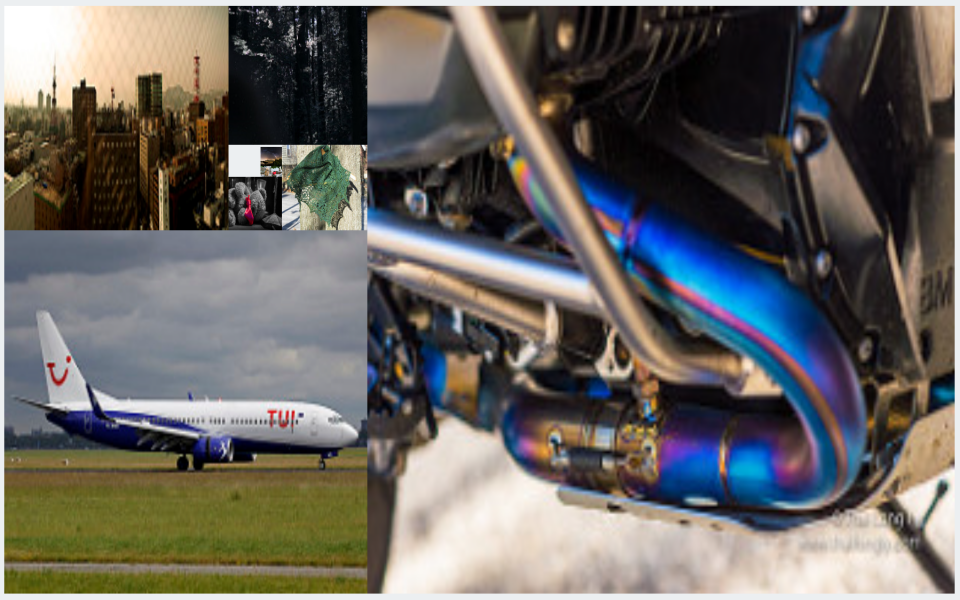
\includegraphics[width=\linewidth]{bluekittenflickr}
\caption[Image spiral `blue kitten'---Flickr]{Image spiral for query `blue kitten'---Flickr}
\label{fig:imgspiralflickr}
\end{figure}

\paragraph{Getty:}
\begin{quotation}
  \begin{description}
  \vspace{-1cm}
    \item[keyword\_ids] Return only images tagged with specific keyword(s). Specify using a comma-separated list of keyword Ids. If keyword Ids and phrase are both specified, only those images matching the query phrase which also contain the requested keyword(s) are returned.
    \item[phrase] Search images using a search phrase.
  \end{description}
  \sourceatright{\autocite{GettyAPI}}
\end{quotation}

Getty uses the \py{phrase} parameter to set the query. It only creates one pataphysicalised query term from the original query and calls for ten results based on that. This decision was based on the quota restrictions\marginnote{§~\ref{s:quota}} defined by Getty. Their limit is based on calls per second rather than calls per day or month. This means we cannot run ten calls for each user query as we did with FLickr. The query ``blue kitten'' gets turned into the word ``racy'' which then calls the \ac{API} to retrieve ten results (see figure~\ref{fig:imgspiralgetty}\marginnote{\faicon{picture-o}~\ref{fig:imgspiralgetty}}). The results mostly show racing cars from various angles although one oddball snuck in too: an office scene Getty has deemed to be `racy' (a guy in a suit checking out a lady's behind while she's leaning over a laptop).

\begin{figure}[!htbp]
\centering
  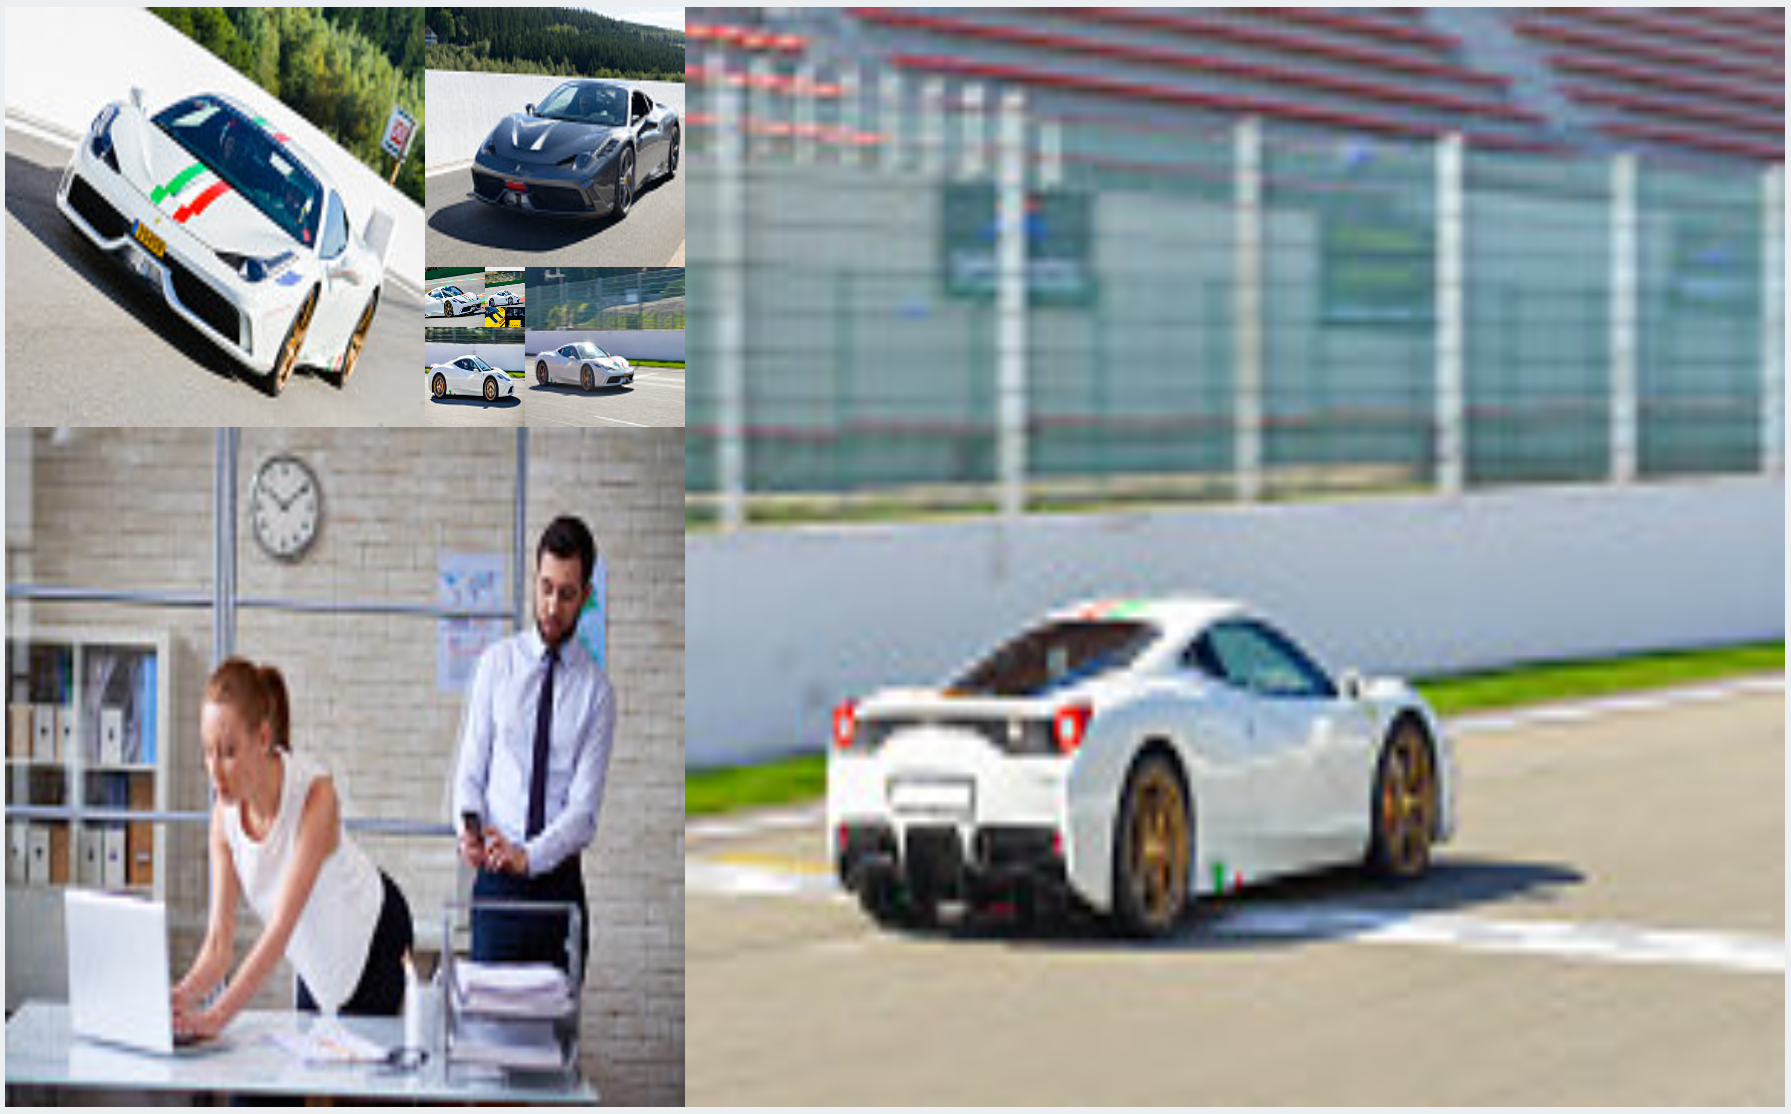
\includegraphics[width=\linewidth]{bluekittengetty}
\caption[Image spiral `blue kitten'---Getty]{Image spiral for query `blue kitten'---Getty}
\label{fig:imgspiralgetty}
\end{figure}

\paragraph{Bing:}
\begin{quotation}
  \begin{description}
  \vspace{-1cm}
    \item[query] The user's search query string. The query string cannot be empty. The query string may contain Bing Advanced Operators\footnote{For example `AND', `OR', `imagesize:', `NOT', or `phrase'}. For example, to limit images to a specific domain, use the site: operator. To help improve relevance and the results, you should always include the user's query string in an insights query (see insightsToken). This parameter is supported only by the Image API; do not specify this parameter when calling the Trending Images API.
  \end{description}
  \sourceatright{\autocite{BingAPI}\footnote{Microsoft will discontinue this version of the current \ac{API} in December 2016. The new version is documented on \url{https://www.microsoft.com/cognitive-services/en-us/bing-image-search-api}.}}
\end{quotation}

The Bing function uses the \py{query} parameter to set the query in the same way as Getty.

\paragraph{YouTube:}
\begin{quotation}
  \begin{description}
  \vspace{-1cm}
    \item[q] The q parameter specifies the query term to search for. Your request can also use the Boolean NOT (-) and OR (|) operators to exclude videos or to find videos that are associated with one of several search terms. For example, to search for videos matching either ``boating'' or ``sailing'', set the q parameter value to boating|sailing. Similarly, to search for videos matching either ``boating'' or ``sailing'' but not ``fishing'', set the q parameter value to boating|sailing -fishing. Note that the pipe character must be URL-escaped when it is sent in your API request. The URL-escaped value for the pipe character is \%7C.
  \end{description}
  \sourceatright{\autocite{YouTubeAPI}}
\end{quotation}

Youtube works in a similar way too. The \py{q} parameter is set to the pataphysicalised query term and one call retrieves ten results.

Something else to consider is perhaps that it is not entirely clear how the internal search for each \ac{API} works. This means that there's a possibility that they do their own query expansion\marginnote{§~\ref{s:qexpansion}} in the background to find more matches.


\subsubsection{Quota}
\label{s:quota}

Each \ac{API} has a different quota for their subscription packages. At this stage this is not a problem but if usage of \url{pata.physics.wtf} were to increase by a lot then these limitations would cause issues. At that point there are two options: (1) live with these limits or (2) get funding to upgrade the subscriptions to these services.

\begin{description}
  \item[Flickr] \num{3600} queries per hour are free \autocite{FlickrGuideAPI}.
  \item[Getty] \num{5} calls per second, unlimited calls per day \autocite{GettyOverviewAPI}.
  \item[Bing] \num{5000} transactions per month are free. A transaction is one request that returns one page of results \autocite{BingAzureAPI}.
  \item[YouTube] \num{50000000} units per day, \num{300000} units per \num{100} seconds per user, and \num{3000000} requests per \num{100} seconds are free. A call to the video search method counts as \num{100} units \autocite{YouTubeAPI}.
  \item[Microsoft Translator] \num{2000000} characters per month are free. Note the quota relates to single characters, not words \autocite{TranslatorAPI}.
\end{description}


\section{Science Fiction}

A more theoretical aspect of this analysis is concerned with what was already discussed to an extent in chapter~\ref{ch:interpretation} (specifically sections~\ref{ss:anthropomorphism}, \ref{s:programmer}, \ref{s:mimicry} and \ref{s:babying}), namely the parallel between artificial creativity and \acl{AI}. 


\subsection{Creativity, Intelligence and Ethics}

Computer creativity falls into the same overarching category as computer intelligence (\ac{AI}) and computer ethics.



John Searle talk at Google (reddit link on phone) \autocite{Searle2015}

epistemic (knowledge)
ontological (existence)

epistemically objectivity (Picasso DOB)
epistemically subjectvity (Picassos value)

ontologically objectivity (material world) - observer-independent
ontologically subjectivity (money, itch, consciousness) - observer-relative

we can study consciousness (ontological subject) in an epistemically objective way.

syntax is not semantics.
Simulation is not duplication.


Natural intelligence is observer-independent, intrinsic, conscious!

Computer intelligence is observer-relative, not intrinsic

"Computer" as in its original meaning: a person who computes, ie the programmer rather than the machine

"All observer relative phenomena are created by human and animal consciousness but the human or animal consciousness that creates them is not itself observer relative."

Computation is not a fact of nature. It's a fact of our interpretation. 

And insofar as we can create artificial machines that carry out computations, the computation by itself is never going to be sufficient for thinking or any other cognitive process because the computation is defined purely formally or syntactically. Turing machines are not to be found in nature, they are found in our interpretations of nature. 

Programs are formal or syntactical. 
Minds have a semantics. 
The syntax by itself is not sufficient for the semantics. 

Steve grant critters


General

Human are more likely to call something AI than they would call something comp creat.






Cohen is the author of AARON, perhaps the longest-lived and certainly the most creative artificial intelligence program in daily use. Cohen viewed AARON as his collaborator. At times during their decadeslong relationship AARON was quite autonomous, responsible for the composition, coloring and other aspects of a work; more recently, AARON served Cohen by making drawings that Cohen would develop into paintings. Cohen's death is the end of a lengthy partnership between an artist and an artificial intelligence.\autocite{Cohen2016}

Cohen had no patience for the ``is it art?'' question. He showed AARON's work in the world's galleries, museums and science centers -- the Tate, the Stedelijk, the San Francisco Museum of Art, Documenta, the Boston Computer Museum, the Ontario Science Center, and many others. His audiences might have been drawn in by curiosity and the novelty of computer-generated art, but they would soon ask, how can a machine make such marvelous pictures? How does it work? The very questions that Cohen asked himself throughout his career.\autocite{Cohen2016}


\todo{aaron stuff}
\url{http://collections.vam.ac.uk/name/cohen-harold/6433/}

\begin{quotation}
  \ldots we'll be seeing an increasing number of artists turning to robotic art of one sort or another in the next five or ten years. We're already seeing some. It's also a pretty safe bet that for the most part they'll be using off-the-shelf robots; that the ``art'' will be manifested in dreaming up contexts they were never intended for; and the culture's definitions of art will change accordingly.
  \sourceatright{\autocite{Cohen2007}}
\end{quotation}

\begin{quotation}
  Shouldn't it be possible, I wondered, to write the rules for generating material for a painting and then simply follow the rules?  In this way, it would be almost as if the painting was painting itself; and I would be relieved of the uncertain task of inventing on a day-to-day basis. 

  That was a little naïve, of course; it simply shifted the burden of invention to another place, another level. I'm still inventing on a day to day basis, but now it's likely to be algorithms for doing particular tasks that I'm inventing.
  \sourceatright{\autocite{Cohen2007}}
\end{quotation}

\begin{quotation}
  I'd like to end with a couple of observations about AARON's algorithm. Firstly; I think it's fair to say that nothing of what has happened could have happened unless I had drawn upon a lifetime of experience as a colorist.  I've evidently managed to pack all that experience into a few lines of code,  yet nothing in the code looks remotely like what I would have been doing as a painter, and AARON's algorithm isn't something a human artist could apply by hand, so to speak.
  \sourceatright{\autocite{Cohen2007}}
\end{quotation}

\begin{quotation}
  It's twenty years since I first realized that I could never turn AARON into a colorist by having it emulate my own expertise; in that case simply because it lacked the hardware upon which that expertise depended. Now I have AARON exercising an algorithm that couldn't be emulated by human colorists, presumably because they lack the hardware to do what AARON does. (and by hardware, in this case I mean the intellectual machinery that can build a stable enough representation and juggle enough variables, as AARON does in running the algorithm.) 
  \sourceatright{\autocite{Cohen2007}}
\end{quotation}

\begin{quotation}
  None of this would be interesting if AARON were an indifferent colorist. But I think I can claim, without undue immodesty, that AARON is a world-class colorist, significantly more inventive and infinitely more productive than I ever was myself. And I conclude that, after decades of expert systems  built to simulate human expertise, AARON has emerged as an expert in its own right. That marks a significant change of state, a change of level, in the never-ending pursuit of autonomy, not merely an incremental change in what the program is able to do. 
  \sourceatright{\autocite{Cohen2007}}
\end{quotation}

\begin{quotation}
  If I were writing AARON's biography today, I might almost say that AARON was a twinkle in its parent's eye in 1963; it was conceived in 1972 but not born until 2006. It has been a long gestation, and right now the parent is struggling to direct an unruly child, keeping it fed and changing its diapers. He has no idea when the child will be potty-trained, much less how long it will be before it reaches adulthood.
  \sourceatright{\autocite{Cohen2007}}
\end{quotation}




Where does this project stand in the wider world and the progress of computing, \ac{AI} and creativity? \ac{AI} and robotics is alluring as a research topic because it is so prevelant in Science Fiction. Computer creativity rarely plays a centrol role though. We can regularly read headlines that tell us that yet another kind of \ac{AI}-bot has won some game against a human player. Or we see videos of some innovative ground-breaking kind of new robot which claims to be near human-like (and yet cannot walk up stairs easily or hold a decent conversation). There are many examples of advances that are hailed as the next big thing which aren't all that great in the grand scheme of things. 

\subsection{AI}
This is also evident in games, for example \ac{VR} and \ac{AR}. The Oculus Rift and similar systems are advertised so much you might believe they are actually about to hit mainstream and every kid will own a \ac{VR} console and headset. Yet they are still way too expensive to be mainstream and motion sickness is also still an issue (and probably always will). These industries are so ``hip'' any publication is seen as the new cool thing without taking into account the history and work that has been done previously in perhaps slightly different disciplines. This is the case for example with a recent article on \ac{VR} sickness and how to compat it. This is a well known problem already---motion sickness already exists in normal games. Similar to epilepsy problems.

\todo{find links for motion sickness}
\todo{find links for epilepsy}
\todo{find links for oculus rift and pokenmon go etc}

\ac{AR} has very recently received a massive boom thanks to Pokenmon Go (released in Australia, New Zealand and the USA in July 2016). It has become a phenomenon since then.
\todo{find pokemon links}

What about IBM's Watson\footnote{See \url{http://www.ibm.com/watson/}}, Microsofts Twitter \ac{AI} chatbot Tay\footnote{See \url{https://web.archive.org/web/20160414074049/https://www.tay.ai/} for an archived version of the original website which is now offline. See also \url{https://twitter.com/tayandyou}, \url{https://www.theguardian.com/technology/2016/mar/24/tay-microsofts-ai-chatbot-gets-a-crash-course-in-racism-from-twitter}, and \url{https://www.theguardian.com/technology/2016/mar/30/microsoft-racist-sexist-chatbot-twitter-drugs}. Wikipedia also has a good article and sources on Tay: \url{https://en.wikipedia.org/wiki/Tay_(bot)}}, Google's AlphaGo\footnote{See \url{https://deepmind.com/alpha-go}} and Hanson Robotics Sophia robot\footnote{See \url{http://www.hansonrobotics.com/}}? How does this relate to my work? Practially of course they are all unrelated. On a deeper level though we can start asking interesting questions. 

https://www.engadget.com/2016/08/07/ibms-watson-ai-saved-a-woman-from-leukemia/
https://xkcd.com/1619/ XKCD WATSON
http://www.wsj.com/articles/SB10001424052748703407304576154313126987674

\begin{description}
  \item[IBM Watson] Watson is a question answering expert system. It famously won against human Jeopardy! champions in 2011.
  \item[Microsoft Tay] 
  \item[Google AlphaGo] AlphaGo is a system for playing the game Go. It won against a top human professional player in 2015.
  \item[Hansen Sophia]
\end{description}

I think these are interesting examples to study since they are supposedly on the forefront of \ac{AI} development. Life-like robots like Sophia still live in the `uncanny valley'. Her voice is creepy and unhuman, her intelligence or her capabilities if understanding conversations are clearly flawed (as shown by her viral remark about supporting genocide).\todo{check} Watson is clever and fast in finding answers for specific questions but he still had problems with humour (e.g. BLAHBLA\todo{find example}) but information lookup is arguably fairly easy and straightforward process within \ac{IR}---sure, it requires processing power and memory storage or access but it is based on simple matching of keywords, not any fancy heuristic algorithms. Microsofts twitter chatbot went viral and users `taught' it nasty swearwords \todo{check} quickly and Microsoft had to take the bot down. It has since apologised although any official documentation on it has disappeared \todo{check}. Google's AlphaGo has been hailed as a breakthrough in \ac{AI} but similar to Watson it is a very targeted and limited program. 

To me it seems the real breakthrough happens when (and if) the first robots appears which isn't as big as a house, can play Go, Chess and hide-and-seek, geniunely manages to get around he uncanny valley effect, has vast knowledge in his memory for instant information lookup, can hold a normal conversation without causing a war, etc, etc---you get the picture. General \ac{AI} is where it's at. Humans can do all the things we do. Children aren't born with only a single function. Imagine a world where humans only have one specialism and can;t do anything else. Mary is a Chess player but can't move her arms. Bob is a medical diagnosis expert but he can't hold a conversation. Movement, speech, memory---they are all vastly complex systems. And I haven't even touched creativity yet.

\todo{whats the point im making? how does this relate to my work?}
Perhpas this `uncanny valley' exists in creativity too. If a robot who looks vaguely human but not quite well enough, or he/she/it sounds almost human but not quite---perhaps if a robot can crack a joke like a human but not quite---perhaps this could be considered uncanny valley too? The philosphical zombies I mentioend in chapter~\ref{ch:interpretation}\marginnote{§~\ref{ch:interpretation}} live in this uncanny valley?

\todo{p and H creativity for computers?}


\subsection{Brains}

I'm not talking about the beer or the zombie food but rather research into the human brain (or animal brains) and attempts to model it on a computer. 

The motivation here is that once we understand how the brain works, perhaps we can understand how certain cognitive processes really work and this of course include creativity.

This is no easy task of course. Chris Chatham talks about ten ``important Differences Between Brains and Computers''\footnote{\url{http://scienceblogs.com/developingintelligence/2007/03/27/why-the-brain-is-not-like-a-co/}} which give a good overview of some of the dificulties of trying to model a brain as is. We can't just do a 1-1 copy.

\begin{quotation}
  \begin{enumerate}
    \item Brains are analogue; computers are digital
    \item The brain uses content-addressable memory
    \item The brain is a massively parallel machine computers are modular and serial
    \item Processing speed is not fixed in the brain; there is no system clock
    \item Short-term memory is not like RAM
    \item No hardware/software distinction can be made with respect to the brain or mind
    \item Synapses are far more complex than electrical logic gates
    \item Unlike computers, processing and memory are performed by the same components in the brain
    \item The brain is a self-organising system
    \item Brains have bodies
    \item	The brain is much, much bigger than any [current] computer
  \end{enumerate}
\sourceatright{Chris Chatham}
\end{quotation}

To bring this into perspective Ray Kurzweil claims the brain is capable of $10^{16}$ operations per second \citeyear[p.194]{Kurzweil2013}. Japan's K-computer (the worlds largest super computer as of 2016) currently has that power---10 petaflops. The ``Blue Brain Project'' is aiming to model $10^17$ bytes of memory and $10^{18}$ flops by 2023 \autocite[p.125]{Kurzweil2013}.
\todo{find k-computer reference}

There are currently some major research projects going on. One of them is the ``Human Brain Project'' \autocite{Walker2012}.

\begin{draft}
quotes:

Our brain consumes about 30W, the same as an electric light bulb, thousands of times less than a small supercomputer. \autocite[p.17]{Walker2012}

For environmental and business reasons, vendors have set themselves the goal of containing energy consumption to a maximum of 20 megawatts  \autocite[p.41]{Walker2012}

the 1 PFlop machine at the Jülich Supercomputing Centre could simulate up to 100 million neurons – roughly the number found in the mouse brain. \autocite[p.41]{Walker2012}

Cellular-level simulation of the 100 billion neurons of the human brain will require compute power at the exascale (1018 flops). \autocite[p.41-42]{Walker2012}

2017 petascale 50petabytes memory + 50 petaflops + <=4MW power

2021 exascale 200petabyte memory + 1exaflop

A second, equally important goal will be to prepare the procurement of the HBP Pre-exascale-supercomputer. By 2017/18, Jülich plans to procure a Big Data-centred system with at least 50 PBytes of hierarchical storage-class memory, a peak capability of at least 50 PFlop/s and a power consumption <= 4 MW. The memory and computational speed of the machine will be sufficient to simulate a realistic mouse brain and to develop first-draft models of the human brain. (The rest of the hardware roadmap targets an exascale machine in 2021/2022 with a capability of 1 EFlop/s and a hierarchical storage-class memory of 200 PB).\footnote{https://www.humanbrainproject.eu/high-performance-computing-platform}

\end{draft}

Why Minds Are Not Like Computers \autocite{Schulman2009}
Software – Hardware == Mind – Brain ??? analogy

"The power of the computer derives not from its ability to perform complex operations, but from its ability to perform many simple operations very quickly."

Layers of abstraction in computers:\\
1.	user interface\\
2.	high level programming language\\
3.	machine language\\
4.	proessor microarchitecture\\
5.	Boolean logic gates\\
6.	transistors\\

layers of abstraction in brain:\\
1.	personality?\\
2.	Thinking?\\
3.	Chemical /electrical signals/activity?\\
4.	Divided Brain regions/structure\\
5.	Neurons\\
6.	Dendrites (input) and axons (output)?\\


Computers are faster and better than humans in many tasks already.

\begin{quote}
"The weaknesses of the computational approach include its assumption that cognition can be reduced to mathematics and the difficulty of including noncognitive factors in creativity." \autocite[p.457]{Mayer1999}
\end{quote}

\todo{find references}
\todo{neural networks and other models based on the brain}

Perhaps we need to have that complete picture of how the brainw orks in order to understand human creativity. I would argue computer creativity is part of general \ac{AI}, and for general \ac{AI} we need massive amounts of general knoweldge.
\todo{common sense research}
\todo{again talk about how this is relevant for my project}
\paragraph{Expert Systems vs General AI}
Is computer creativity an expert system or does it fall into general \ac{AI}? 

\paragraph{Machines self-assessing}
Perhaps there is an argument that if humans are the only entities who can judge whether another human is being creative, then machines should be assessing themselves. This is a paradoxical concepts though. Since machines are products made my humans, they can never be autonomous in that sense. If machines had evolved like other animals besides us this argument might hold but obviously that is not the case.


\section{Design}

It is interesting to note how different the search results are perceived when presented in a different style (e.g. list rather than poem). This could be studied using questionnaires and interviews or eye tracking tools to find out what users prefer or perceive as more creative for example (see chapter~\ref{ch:aspirations},~\ref{ch:aspirations}). 

Figures~\ref{fig:poemtree},~\ref{fig:listsourcetree}~and~\ref{fig:listalgotree} show the three different text result styles. The poetry\marginnote{\faicon{picture-o}~\ref{fig:poemtree}} is compact and invites users to read all \num{14} (or less) lines. The two list styles\marginnote{\faicon{picture-o}~\ref{fig:listsourcetree}~\&~\ref{fig:listalgotree}} are much longer and involve a lot of scrolling to navigate, which might deter users from actually reading many of the results.

\begin{figure}[!htbp]
\centering
  \includegraphics[width=\linewidth]{poemtree}
\caption[Results as poem]{Results in poem form for query `tree'---Shakespeare}
\label{fig:poemtree}
\end{figure}

\begin{figure}[!htbp]
\centering
  \includegraphics[width=\linewidth]{listsourcetree}
\caption[Results as list by sources]{Results as list by sources for query `tree'---Shakespeare}
\label{fig:listsourcetree}
\end{figure}

\begin{figure}[!htbp]
\centering
  \includegraphics[width=\linewidth]{listalgotree}
\caption[Results as list by algorithm]{Results as list by algorithm for query `tree'---Shakespeare}
\label{fig:listalgotree}
\end{figure}


\section{Meta}

\subsection{Management}
\todo{add file for appendix with full git history}

On a different note, the project was completed over X years which includes an interruption and later on only a part time commitement.

I kept the project in a ``git repository''. Git is a version ontrol system that allows users to roll-back on changes and I further pushed my work to GitHub to make sure hardware failure or human error (i.e. lost or stolen property) would not affect my work. 

To understand git you need to know what commits are. They are the thing where I save my current state of the project and give it a description.

Below you can see a shortened version of the timeline of my commits between 20XX and the time of submission of this thesis. A full version can be found in appendix XYZ. You can see from this the time between programming work I did on \url{pata.physics.wtf} and its predecessors.

\todo{add calendar screenshot of github contributions}
\todo{links to git and github}

\begin{verbatim}
  *   10f61f9  Sun 08 May 2016	 (HEAD -> api, origin/api) Merge remote-tracking branch 'refs/remotes/origin/master' into api
  |\  
  * | 71437f6  Tue 18 Aug 2015	 Flickr and Bing work, radio buttons work
  * | 6c552aa  Wed 12 Aug 2015	 Fixed image problem but not video.
  | | * 1cbb63d  Tue 11 Aug 2015	 (origin/thesis) Update textsurfer.py
  | |/  
  |/|   
  * | 0ebff0d  Tue 11 Aug 2015	 Analytics enabled again
  * | 703f977  Tue 11 Aug 2015	 Problems solved.
  * | 74a1fae  Tue 11 Aug 2015	 About to change l\_dict to dict of dict
  * | 0935b23  Mon 10 Aug 2015	 BUG FUCKER
  * | 4f7d91e  Mon 10 Aug 2015	 Turn debug off
  * | 58f0c2b  Mon 10 Aug 2015	 Button styling done
  * | 59add58  Mon 10 Aug 2015	 Email problem solved
  * |   f1b2d40  Sun 09 Aug 2015	 Merge branch 'Deploy' into thesis
  |\ \  
  | * | 435cb2d  Sun 09 Aug 2015	 Deployment works, added analytics
  | * | 8a63dc7  Sat 08 Aug 2015	 gunicorn runs locally fine.
  | * | 2861407  Sat 08 Aug 2015	 Revert 5f2c957..4026965
  | * | 4026965  Sat 08 Aug 2015	 Tests
  * | |   8f2eeab  Sat 08 Aug 2015	 Merge branch 'w3' into thesis
  |\ \ \  
  | |/ /  
  | * | 5f2c957  Sat 08 Aug 2015	 Stuff
  | * | 873153c  Fri 07 Aug 2015	 Tiny cleanup
  | * | 05d5760  Thu 06 Aug 2015	 Random Poems and Emailing works
  | * | 657126c  Wed 05 Aug 2015	 Random poems work - without links though
  | * | 3d31ea9  Wed 05 Aug 2015	 Randomise still only works once, count ok
  | * | 5f1d45b  Wed 05 Aug 2015	 Randomise poem works ONCE
  | * | c583341  Wed 05 Aug 2015	 Poem subtabs, email poems done
  | * | f1b3878  Wed 05 Aug 2015	 Hiding divs
  | * | a6939c4  Tue 04 Aug 2015	 huh?
  | * | e6b411d  Tue 04 Aug 2015	 Poem emails WORK Fuck YEAH!
  | * | 4b6b170  Tue 04 Aug 2015	 Test email
  | * | 24e356c  Tue 04 Aug 2015	 Better load icon
  | * | e6ae736  Tue 04 Aug 2015	 loading icon version 1
  | * | 51b43e2  Tue 04 Aug 2015	 Added 4th pictures
  | * | f2d8a83  Mon 03 Aug 2015	 Minor fixes
  * | |   1ddb03d  Mon 03 Aug 2015	 Merge branch 'w3' into thesis
  |\ \ \  
  | |/ /  
  | * | ca4eab3  Mon 03 Aug 2015	 Pretty good state.
  | * | 9370334  Mon 03 Aug 2015	 working on list display of images
  | * | e1f1ead  Mon 03 Aug 2015	 Stylesheets sorted and cleaned files
  * | |   9732d5b  Mon 03 Aug 2015	 Merge branch 'w3' into thesis
  |\ \ \  
  | |/ /  
\end{verbatim}

\spirals

I also kept the thesis under git version control. Since the thesis was written in \LaTeX you could almost say I `programmed' it. Below is an outline of the commit history for this thesis.

\begin{verbatim}
* 3f06260	 Edited readme again
* c721b33	 Edited readme
* ffbdb4b	 Edited readme
* 8870b3d	 Added gitignore file
* ba1a9c2	 Second commit
* 244c4b3	 First commit
\end{verbatim}


\subsubsection{Development}

doing the analysis really helped revising and improving the code.



\subsection{Thesis}

\subsubsection{Part Spirals}

Each new thesis part contains a word spiral based on a poem generated by \url{pata.physics.wtf} using the a part of the title as keyword. They represent the pataphysical (Archimedean) spiral.

\begin{enumerate}
  \item Preface --- \emph{pre}
  \item Hello World --- \emph{hello}
  \item Tools of the Trade --- \emph{trade}
  \item The Core: Techno-Logic --- \emph{core}
  \item The Core: Techno-Practice --- \emph{practice}
  \item Meta-Logicalysis --- \emph{meta}
  \item Happily Ever After --- \emph{after}
  \item Postface --- \emph{post}
\end{enumerate}

\subsubsection{Chapter Poetry}

Each chapter opens with a poem generated by \url{pata.physics.wtf} using a part of the chapter title as keyword.

\begin{enumerate}
  \item Introduction --- \emph{intro}
  \item Inspirations --- \emph{inspiration}
  \item Methodology --- \emph{method}
  \item Pataphysics --- \emph{pata}
  \item Creativity --- \emph{creativity}
  \item Technology --- \emph{technology}
  \item Evaluation --- \emph{evaluation}
  \item Foundations --- \emph{foundation}
  \item Interpretation --- \emph{interpretation}
  \item Implementation --- \emph{implementation}
  \item Applications --- \emph{application}
  \item Patanalysis --- \emph{patanalysis}
  \item Aspirations --- \emph{aspirations}
  \item Observations --- \emph{observations}
\end{enumerate}

\todo{say more, check keywords, potentially generate new poems}





\section*{creative analysis}
\begin{draft}
  literary deconstruction and recombining to make new creative output? \\
  perception of results (poetry, source, algorithm) \\
  discuss applications from before (stimulates creative detour away from the obvious) \\

  How does this relate to Oulipo and Pataphysics? 

  Perhaps this is where I should talk a bit about the perception of results in their different output formats/styles. The poetry is automatically read with more gravity. Sorting by sources is a game of exploration or algorithms which becomes a game of finding the similarities within the result sets. They are different ways to view the same things and yet have a drastic influence of how the results are perceived. This also applies to the image and video search. Presenting results in spiral form is weird. Its hard to see where one image ends and another starts, they just kind of blur into each other. When listed as a list they immediately become more boring.

  talk abit about what the original plan was for some of the big changed elements in the website, e.g. the image search running 10 times on different keywords rather than running once with 10 results for the same keyword.
\end{draft}


DELETE EVERYTHING FROM BELOW HERE:


\begin{draft}
DELETE THIS

In this section we consider the possible uses and applications for the proposed creative search tool.

Our target audience is not quite as broad as that of a general search engine like Google. Instead, we aim to specifically cater for users who can appreciate creativity or users in need of creative inspiration. Users should generally be educated about the purpose of the search tool so that are not discouraged by what might appear to be nonsensical results. Users could include artists, writers or poets but equally anybody who is looking for out-of-the-box inspirations or simply a refreshingly different search engine to the standard.

The way we display and label results produced by the tool can influence how the user perceives them. The current prototype for example separates the results into its three components but we could have equally just mixed them all together. The less transparent the processes in the background (e.g.\ which algorithm was used, how does the result relate to the query precisely, etc.) are for the user, the more difficult it might be to appreciate the search.

There are many ways a pataphysical search tool could be used across disciplines.

In literature, for example, it could be used to write or generate poetry, either practically or as a simple aid for inspiration. We are not limited to poetry either; novels, librettos or plays could benefit from such pataphysicalised inspirations. One can imagine tools using this technology that let you explore books in a different ordering of sentences (a sort of pataphysical journey of paragraph hopping), tools that re-write poems or mix and match them together. Even our simple prototype shows potential in this area and could be even more powerful if we extended it to include more base texts, for example the whole set of books contained in Faustroll’s library ([20] and also [12]). A richer body of texts (by different authors) would produce a larger index which would possibly find many more matches through WordNet and end in a more varied list of results.

From a computer science perspective it could be used as one of the many algorithms used by traditional search engines for purposes like query feedback or expansion (e.g. “did you mean … “or “you might also be interested in … “). Depending on how creative we want the search engine to be, the higher we would rank the importance of this particular algorithm. One of the concepts related to the search tool, namely patadata, could have an impact on the development of the Semantic Web. Just as the Semantic Web is about organizing information semantically through objective metadata, patadata could be used to organize information pataphysically in a subjective way.

The prototype tool is already being used in the creation of an online opera, provisionally entitled from [place] to [place], created in collaboration with The Opera Group, an award-winning, nationally and internationally renowned opera company, specialising in commissioning and producing new operas. In particular, it is being used to create the libretto for one of the virtual islands whose navigation provides the central storyline for the opera. The opera will premiere in 2013, and will continue to develop thereafter, deploying new versions of the tool as they appear.
\end{draft}






\stopcontents[chapters]


\phantomsection
\addcontentsline{toc}{part}{HAPPILY EVER AFTER}
\partimage[width=\textwidth]{spiral_after.pdf}
\part{\texorpdfstring{H$\forall$PPILY $\Sigma$V$\Sigma$R $\forall$FT$\Sigma$R?}{HAPPILY EVER AFTER?}}
% % !TEX root = ../main.tex

\chapter{Aspirations}
\label{ch:future}

\startcontents[chapters]

\vfill

\begin{alltt}\sffamily
Mid the silence that pants for breath,
when I thought myself at my last gasp,
haine ou de l'ambition et qui se,
the pale motor vessel withdrew its blue breath toward the island's horizon.

As pure and simple as a powder puff,
such also was the ambition of others upon the like occasion,
there was hardly a breath of air stirring,
mon ancien cœur en une aspiration vers la vertu.

After drawing a long breath,
the silver ring she pull'd,
the suitor cried, or force shall drag thee hence.

For wild ambition wings their bold desire,
and with thine agony sobbed out my breath,
I will pull down my barns.
\end{alltt}

\newpage
\minicontents
\spirals


Developing a software product rarely finishes. It is maintained, refactored, repurposed, updated, extended, etc. Especially with creative products, where the functional requirements are more fluid perhaps, it is always tempting to change things. 

For the purpose of this doctoral project, the artefact \url{pata.physics.wtf} is a snapshot of a product in constant motion. The state of the code at the time of submission of this thesis is described in chapter~\ref{ch:implementation}\marginpar{§~\ref{ch:implementation}} and further elaborated on in the \nameref{ch:analysis} chapter\marginpar{§~\ref{ch:analysis}}. But it may very well continue to evolve.

Here, in this chapter I will lay out some of the potential further work for this project. This may continue on a private basis or in a more academic environment. 


\section{Performance}
\label{s:performance}

\paragraph{Startup} 
The website can be slow to load. Currently speed performance was not a priority during development. In fact it is not built for speed from the ground up. Each time the server restarts, the indexing process takes place from scratch (see chapter~\ref{s:setup}\marginpar{§~\ref{s:setup}}). This takes time. Google and other big web search engines do this continuously in the background to keep data up to date. The index\marginpar{§~\ref{s:index}} is currently cached after startup but perhaps preprocessing it and storing it more permanently in a database would help speed up the start. However this may not be necessary, as it only affects the server startup.

\paragraph{Query Response} 
The time it takes from the user entering a query term and the system displaying the results page varies between unnoticable short and impatiently long. This is due to the pataphysicalisation process. This requires calls to external and internal \ac{API}s such as Flickr and WordNet. See analysis on speed issues in table~\ref{tab:percent}\marginpar{\faicon{table}~\ref{tab:percent}}.

\paragraph{Preprocessing Corpora} 
At this point the texts in the corpora consist of almost unedited plaintext (`.txt') files\footnote{For text files downloaded from Project Gutenberg, the Gutenberg specifc copyright notices have been removed to only contain the relevant body of text.} (see chapter~\ref{s:corpora}\marginpar{§~\ref{s:corpora}}). Newlines and whitespace formatting varies, as does language and quality of spelling. Generally, chapter headings, chapter numberings, etc. were left untouched. The Shakespeare corpus contains poetry and plays for example. With the plays, scene information, stage directions, and voice details were kept. This means sentences that appear in the results of the search tool can contain peripheral words such as in this example: ``\ldots Athens and a wood near it ACT I \ldots'' from \textit{A Midsummer Night's Dream} or this example: ``\ldots Exit SHERIFF Our abbeys and our priories shall pay This expedition's charge \ldots'' from \textit{King John}. This could be addressed by preprocessing the individual texts in advance and removing any text that might interfere with the readablility of results.

\paragraph{Image Sizes} 
At the moment images are retrieved at one specified size through the various \ac{API} calls even though they are displayed at various different sizes depending on their location in the image spiral (unless they are displayed as a list). This process could certainly be optimised. Smaller image sizes could be accessed via the \ac{API}s.


\section{Design}
\label{s:designaspi}

\paragraph{Responsive Spirals} 
Currently the image and video spirals (see chapter~\ref{s:imgvid}\marginpar{§~\ref{s:imgvid}}) are fixed size. This means that when the webpage is resized the spiral stays the same size and is left-aligned on the page. Ideally it would be better to scale the spiral with the width of the browser page. This could be achieved using percentage widths, although it would require a lot of work to adapt the current code for the spirals (see chapter~\ref{s:imgspiral}\marginpar{§~\ref{s:imgspiral}}).

\paragraph{Scalable Image Sizes} 
As mentioned above, images are retrieved at one size through the various \ac{API} calls. Because images in the spiral have different sizes according to where in the spiral they are located, they are scaled up or down directly in the \ac{HTML} code. This means that some of the images look distorted and pixelated if they have to be scaled up or down too much.

\paragraph{Square Aspect Ratio} 
Another issue is the aspect ratio of images and videos. For the spiral they need to be square. They are currently distorted as opposed to cropped. It might be possible to specify an option in the \ac{API} calls to only retrieve square images which would help this problem.

\paragraph{Responsive Poems} 
A similar problem to the responsive spirals exists with the display of the Queneau poems. The random poems are centered on the page but the Queneau poems require a lot more formatting and styling to render and currently this is achieved by left-aligning them and having a fixed `absolute' position on the page. Ideally this would also be centered as in the random poems. 

\paragraph{Paginate Results}
For the text-by-source and text-by-algorithm search as well as the image- or video-as-list search results, it may improve the loading speed of the results page to split the results into smaller chunks and display them on several pages instead of one long scrolling page. This is called pagination.

\paragraph{Random Sentences} 
Adding to the source of random sentences used in the top and bottom banner on the website should be an ongoing endeavour. The current list of sentences used is shown in appendix~\ref{s:appsentences}\marginpar{§~\ref{s:appsentences}}.


\section{Text}
\label{s:textfuture}

\paragraph{Result Sentences} 
Currently the way result sentences are retrieved for the text search is based on punctuation (see chapter~\ref{s:ressent}\marginpar{§~\ref{s:ressent}}). This means once a pataphysicalised keyword has been found, the system retrieves up to \num{10} words prior until it reaches a punctuation mark and the same for after. The idea here was to get suitable sentence fragments. This could be changed to rely on \ac{POS} tags for example or simply retrieving complete sentences.

\paragraph{Stopwords}
When the index is created only words that are not considered stopwords are added. We could modify the list of stopwords (see appendix~\ref{s:stopwords}\marginpar{§~\ref{s:stopwords}}) to include a few more uninteresting words. Or we could simply remove everything but nouns for example. This would drastically influence the results produced by the system.

\paragraph{Rhyming Scheme} 
One of the biggest points for future work is to introduce a rhyming scheme for the poetry results. This might involve some more \ac{NLP} during the creation of the index\marginpar{§~\ref{s:index}}. It would make the poems much more readable. This could include pronounciation \ac{POS} tags or other \ac{IPA} like data (for example using an \ac{API} like Wordnik \autocite{Wordnik2016} or a library like \ac{NLTK}). So a word in the index dictionary might contain the following items.

\begin{minted}{text}
  (``tree'': [``l_00'': [24,566,4990], ``s_14'': [234,5943]], ``[tri]'')
\end{minted}

By doing \ac{POS} tagging\marginpar{§~\ref{s:pos}} with pronounciation data, we could retrieve sentences that match the sound of the last word of the previous line for example.


\section{Pataphysicalisation}
\label{s:pataasp}

\paragraph{WordNet}
The vocabulary in WordNet is limited. According to its website \autocite{Princeton2010} it contains \num{117000} `synsets'\footnote{Synonyms---``words that denote the same concept and are interchangeable in many contexts''---are grouped into unordered sets called synsets \autocite{Princeton2010}.} This affects two of my algorithms (namely the Syzygy and Antinomy algorithms). See also discussion in chapter~\ref{s:analsyzygy}\marginpar{§~\ref{s:analsyzygy}}. An option might be to somehow widen the amount of word matches by including different word-types/forms and relationships, such as troponyms, homonyms and heteronyms. Using these could introduce a whole new kind of pataphysical result. 

Homonyms are pronounced the same but mean something else (e.g. `write' and `right'). Heteronyms are words that are spelled the same but have a different meaning (e.g. `close to the edge' and `to close the door'). Homophones are often used to create puns (and remember---puns are syzygys of words), for example ``past your eyes'' and ``pasteurize''. 

\begin{quotation}
   You can tune a guitar, but you can't tuna fish. Unless of course, you play bass. \sourceatright{(attributed to Douglas Adams)}
\end{quotation}

\paragraph{Antinomy}
The antinomy algorithms relies on WordNet's antonyms. A lot of words simply do not have an opposite and no fallback is currently defined. This means a lot of the time the antinomy function will not produce any results. Andrew Dennis implemented the algorithm in the same way, as discussed in chapter~\ref{s:dennis}\marginpar{§~\ref{s:dennis}}. It would be great to come up with a better way of dealing with this concept to ensure results are produced everytime.

\paragraph{Stemming}
Stemming could increase the number of results found by all algorithms (see chapter~\ref{s:nlp}\marginpar{§~\ref{s:nlp}}). A danger of increasing the output of the pataphysicalisation is always that results become more boring. Currently queries such as `clear' and `clearing' are treated as separate entities and would produce different results. Stemming would turn both of these words into the stem `clear' and they would return the same results. Now it becomes immediatly clear (no pun intended) though that this might not always be desirable as just illustrated in this sentence: the root meaning of `clear' can be very different to the meaning of `clearing'.

\paragraph{Queneau's poems}
It would be nice to actually add Queneau's poems \autocite{Queneau1961} into the Faustroll corpus as little easter egg (see chapter~\ref{s:culture}\marginpar{§~\ref{s:culture}}).

\paragraph{Image Algorithms}
The image and video search currently rely on external \ac{API}s (see chapter~\ref{s:imgvid}\marginpar{§~\ref{s:imgvid}}). One option to approach this in a totally different way would be to write algorithms that analyse and pataphysicalise the actual image or video data themselves. This might involve manipulating histograms or pixel maps.

\paragraph{Maximum Obscurity}
N-grams are a \ac{NLP} technique introduced in chapter~\ref{s:ngrams}\marginpar{§~\ref{s:ngrams}}. The idea is that it allows for prediction of likely word pairs, meaning if the word `sunny' often occurs just before the word `day' in a given training text or corpus then the probability for this particular n-gram is higher than say for `sunny dog'. This can be increased to predict the probability of longer chains of words. One can immediately see the attraction of abusing this to generate pseudo sentences or even of creating a formula similar in nature but for example ranking obscure combinations of words higher than common ones. So for example instead of having a \acf{MLE} (see equation~\ref{eq:mle}\marginpar{$\bm{\Sigma}$~\ref{eq:mle}}) we could have a `Maximum Obscurity Estimation' which returns the highest probabilty for word sequences that happen the rarest.

\paragraph{Pataphysical Entropy}
Similarly, we could play with maximum entropy models as shown in chapter~\ref{s:maxent}\marginpar{§~\ref{s:maxent}} together with \ac{POS} tagging\marginpar{§~\ref{s:pos}} by rigging given probability for tags. There are endless possibilities of abusing these kinds of techniques. This is also very reminiscent of \ac{OULIPO} techniques. 

\paragraph{Grammars}
We could create a whole new language grammar based on pataphysical principles. Examples of using a standard grammar (see chapter~\ref{s:grammars}\marginpar{§~\ref{s:grammars}}) for generating `random' text are as follows\footnote{\autocite{Winter2016,Dada2016,Stribling2016}}.

\begin{adjustwidth}{1cm}{}
\begin{description}[leftmargin=3cm]
  \item[ArtyBollocks] Generates artist statements.
  \item[DadaEngine] A system for generating random text from grammars.
  \item[SciGen] Generates random Computer Science research papers.
\end{description}
\end{adjustwidth}

\paragraph{Uncreativity}
In chapter~\ref{s:csf}\marginpar{§~\ref{s:csf}} I discussed the concepts of uninspiration and aberration by Wiggins and Ritchie \autocite*{Wiggins2006,Ritchie2012} in relation to their \ac{CSF}. We could define a `Pataphysical Search Framework' in the same way. Table~\ref{tab:csf}\marginpar{\faicon{table}~\ref{tab:csf}} shows some of their original definitions for various forms of aberration and uninspiration. Table~\ref{tab:patacsf}\marginpar{\faicon{table}~\ref{tab:patacsf}} then shows some rough ideas about how pataphysical concepts might be defined.

\begin{adjustwidth}{1cm}{}
\begin{description}[leftmargin=2.5cm]
  \item[Clinamen] smallest possible aberration to make the biggest difference
  \item[Antimomy] reachable, abnormal concepts with value
  \item[Anomaly] reachable concepts outside the norm
  \item[Absolute] criteria for value and norm must be perfectly matched
  \item[Syzygy 1] concepts reachable within 3 steps from the query
  \item[Syzygy 2] transformed set of concepts $S_{obj} \rightarrow S^{meta} \rightarrow S'{obj}$
\end{description}
\end{adjustwidth}

This is definitely work in progress and it would be out of the scope of this thesis to elaborate much further.

\begin{table}[!htbp]
\centering
\caption{CSF concept definitions of uncreativity (see chapter~\ref{s:csf})}
\label{tab:csf}
\begin{tabu}{ll}
\toprule
\textbf{Name} & \textbf{Equation} \\
\midrule
Universal set of concepts & $U$ and $X \subseteq U$ \\
Aberration & $B \text{ where } B \notin N_\alpha (X) \ \wedge \ B \neq \emptyset$ \\
Perfect Aberration & $V_\alpha (B) = B$ \\
Productive Aberration & $V_\alpha(B) \neq \emptyset \ \wedge \ \neq B$ \\
Pointless Aberration & $V_\alpha(B) = \emptyset$ \\
Hopeless Uninspiration & $V_\alpha (X) = \emptyset$ \\
Conceptual Uninspiration  & $V_\alpha (N_\alpha (X)) = \emptyset$ \\
Generative Uninspiration  & $elements(A) = \emptyset$ \\
\bottomrule
\end{tabu}
\end{table}

\begin{table}[!htbp]
\centering
\caption[CSF pataphysical concepts]{Possible definitions of pataphysical concepts in terms of the CSF}
\label{tab:patacsf}
\begin{tabu}{XX[5]} 
\toprule
\textbf{Name} & \textbf{Equation} \\
\midrule
Norm & $N_\alpha (X) = \{c \in X \ | \ N(c)> \alpha\} \text{ where } N \in [0,1]^X$ \\
Value & $V_\alpha(X) = \{c \in X \ | \ V(c) > \alpha\} \text{ where } V \in [0,1]^X$ \\
Pata & $P_\alpha(X) = $ \newline $\{c \ | \ c \in(CLI(X)\cup ANT_\alpha(X) \cup SYZ(X) \cup ANO_\alpha(X) \cup ABS(X))\}$ \\
Clinamen & $CLI(X) = \{c \in X \ | \ N_{0.9} (N_{0.1} (c))\}$ \\
Antinomy & $ANT_\alpha(X) = \{c \in X \ | \ V(N_0(c)) > \alpha\}$ \\
Anomaly & $ANO_\alpha(X) = \{c \in X \ | \ N(c)< \alpha\}$ \\
Absolute & $ABS(X) = \{c \in X \ | \ V_1 (N_1 (X)) \neq \emptyset\}$ \\
Syzygy 1 & $SYZ(query) = \bigcup_{n=0}^{3} elements(Q(N,V)^n (query))$ \\
Syzygy 2 & $SYZ(X) = S'(X) \text{ where } S_{obj} \rightarrow S^{meta} \rightarrow S'{obj}$ \\
\bottomrule
\end{tabu}
\end{table}


\section{Extensions}
\label{s:extensions}

\paragraph{Additional APIs} 
Currently 5 \ac{API}s\footnote{Flickr, Getty, Bing, MicrosoftTranslator and YouTube} are used in \url{pata.physics.wtf}. This could be increased to include more varied sources of data. Sites like Flickr are heavily based on user tags (`folksonomies') which can be unreliable and a bit random at times. Possible additional \ac{API}s to consider would be Instagram, Imgur, Facebook, Google Image Search, DeviantArt, Pinterest, Vimeo, Twitter, SoundCloud, etc.

\paragraph{Web Search} 
The use of \ac{API}s could also include web search results rather than just images and videos. This would need its own interface section and a suitable display style for the results. The biggest problem for this are \ac{API} limitations as mentioned in chapter~\ref{s:apis}\marginpar{§~\ref{s:apis}}. Alternatively a ready-made index or crawl could be used but these are typically many terrabytes in size and have a cost attached. Crawling the web myself is not an option due to the computational power, time and space required to do so.

\paragraph{Additional Algorithms} 
It would be nice to implement some more algorithms for the search tool. This could include the two additional algorithms suggested by Andrew Dennis (see chapter~\ref{s:dennis}\marginpar{§~\ref{s:dennis}}) or developing more of my own. This could involve implementing some of the other pataphysical principles, such as equivalence or anomaly. Or it could consist of implementing some of the more famous \ac{OULIPO} techniques. The repertoire of them is huge (see tables~\ref{tab:oulipo1} and \ref{tab:oulipo2}\marginpar{\faicon{table}~\ref{tab:oulipo1} \& \ref{tab:oulipo2}}).

\paragraph{Custom API}
Finally, it would be great to develop a custom \ac{API} for the algorithms of \url{pata.physics.wtf}. This would allow other people to use the search remotely without going through the interface and to use the results as they want. This would have been beneficial for the Digital Opera project\marginpar{§~\ref{s:opera}} and certainly for other researchers/developers like Andrew Dennis\marginpar{§~\ref{s:dennis}}.


\section{User Testing}

\paragraph{Focus Group}
It might be interesting to look at opinions of various people (general public and experts) about the interpretation/evaluation framework. This could be done by asking them to provide their own definition of computer creativity and then to analyse and evaluate a product (such as \url{pata.physics.wtf}) according to their own criteria. Then follow this up by getting the same people to use my proposed framework\marginpar{§~\ref{s:framework}} to compare the results. This would include asking them about whether or not they thought that using the framework was beneficial to them or confusing.

\paragraph{Eye-Tracking}
To study the effects of using different styles of presenting the same results, an eye-tracking experiment could be done. This would involve setting up participants with the necessary equipment and then introduce them to \url{pata.physics.wtf} and moniter their eye movements as they navigate the site. This could also provide details about how long users spend on each results page, what kind of style of results they prefer, etc. Some may prefer image or video search over the text search while others may not be interested in that at all. Generally of course one has to take into account that this is a creative piece of work and not everybody will like it. It is purposefully purposeless and highly subjective, so user feedback may not provide unbiased and useful results.


\section{Audio}
\label{s:audio}

It would be nice to include audio search using an \ac{API} such as SoundCloud. Technically the pataphysicalisation could work similar to the image and video searches, meaning it would be based on user tags. One idea would be to work with audio waves directly although this needs to be explored further first.


5K PURSUIT OPERA (1992)  
Acclaimed TV opera. Sport interacts with art through digital score. Channel 4 Television
http://www.dmu.ac.uk/about-dmu/academic-staff/art-design-humanities/pip-greasley/pip-greasley.aspx



john cage 4'33'' 


andrew hugill


\section{From the Aspirations to Paris by Sea}

\begin{figure}[!htb]
\centering
  \includegraphics{aspi.pdf}
\end{figure}



\begin{figure}[!htb]
\centering
  \includegraphics[width=\textwidth]{legend.pdf}
\end{figure}

\stopcontents[chapters]

% % !TEX root = ../main.tex

\chapter{Outroduction}
\label{ch:observations}

\startcontents[chapters]

\vfill

\begin{alltt}\sffamily
Yet my state is well,
is to take those things for bird,
and God keep him out of my sight,
I do spy some marks of love in her.

With catlike watch,
I have watch'd and travell'd hard,
and some will mourn in ashes,
so that hardly can I check my eyes from tears.

Pillars of the state,
word out of his right sense,
first emperor of Rome Mark Anthony.

Have you had quiet guard,
though art a guard too wanton for the head,
of each other's watch.
\end{alltt}

\newpage
\minicontents
\spirals

\todo{summarise thesis, contributions etc. conclude by comparing against introduction}

a wide range of subject areas such as computer science, psychology, linguistics, literature, art and poetry, languages and mathematics.
\todo{refer back to these in conclusion}


\section{Observations}

The last XYZ chapters have explained in probably too much detail what \ac{AMC} is and how to evaluate it. Given that this spans so many different disciplines the contextual background information necessary to understand the research was presented in a broad literature survey in chap XYZ. This also posed a problem for choosing the right methodology for the project. In the end a transdisciplinary approach was chosen as described in chap XYZ with a heavy component of iterative exploratory rapid-prototyping to develop an artefact to demonstrate what \ac{AMC} is. 

This artefact is presented on \url{pata.physics.wtf}. It is an artwork dedicated to \ac{AMC}, pataphysics, \ac{OULIPO} and programming culture.

A critique of computer creativity and its current evaluation formed the starting point for a new framework which was introduced in chap XYZ. The general conlcusion of the thesis was made up of the critical analysis and further work chapters as awell as this final concluding chapter right at the end.

The appendix contains various code snippets and peripheral pieces vaguely related or relevant for parts of this thesis. The code of the website is included on a CD CHECK attached to the back of the front cover. Of course the website is also available online at \url{pata.physics.wtf}.

\todo{check if i need to submit a CD?}


\section{Issues}

\begin{itemize}
  \item Summarise issues in analysis Section
  \item summarize future work
\end{itemize}


\section{Answers}
\label{s:answers}

In the introduction I asked several questions that I attempted to asnwer with my research. This section contains brief answers from 50.000 feet\footnote{Inspired by Time Berners-Lee's articles on the Web in 1998---/url{http://www.w3.org/DesignIssues/Architecture.html}}, meaning they provide a top-down view of the answer and pointers to where in the thesis readers can find more elaborations.

\todo{add chapter references}
\todo{these are closed questions, not research questions}
\begin{description}
  \item[Can computers or algorithms be considered creative?] In short: no. In chapters~\ref{ch:evaluation}\marginnote{§~\ref{ch:evaluation}} and~\ref{ch:interpretation}\marginnote{§~\ref{ch:interpretation}} I have gone into great detail of why I believe that this cannot happen any time soon (see argument of zombies). They can be `creative' (adj/adv CHECK) but the source of the creativity is the programmer of the machine not the machine itself.
  \item[Can pataphysics facilitate creativity?] Yes. Pataphysics provides many principles which can be turned into technicques and constraints which is well known to be able to support creativity (see chapter~\ref{ch:foundations}\marginnote{§~\ref{ch:foundations}}). This is also evident in the \ac{OULIPO} and their use of constraints (see chapter~\ref{ch:creativity}\marginnote{§~\ref{ch:creativity}}).
  \item[Can a creative process be automated or emulated by a computer?] Yes, in theory. It mainly depends how you define the creative process and that is fairly subjective. See more in chapter~\ref{ch:creativity}\marginnote{§~\ref{ch:creativity}} and~\ref{ch:interpretation}\marginnote{§~\ref{ch:interpretation}}.
  \item[Can human and computer creativity be objectively measured?] No. As discussed in chapter~\ref{ch:interpretation}\marginnote{§~\ref{ch:interpretation}} since the perception of creativity is subjective it cannot be quantified in objective terms. By providing a framework\marginnote{§~\ref{s:oec}} that takes into account all possible contextually relevant contributors though we can approximate an objective evaluation.
  \item[Can information retrieval be creative?] Yes. There are many ways this can be achieved too as mentioned in chapter~\ref{ch:analysis}\marginnote{§~\ref{ch:analysis}}.
  \item[Can search results be creative rather than relevant?] Yes, although this is also subjective. What is creative to some might not be creative to everybody. The artefact also nicely showed the difference in perception of results simply based on design of the content (see chapter~\ref{ch:analysis}\marginnote{§~\ref{ch:analysis}}).
\end{description}



\section{Contributions}

mention to whom these could be useful

\todo{write more}

This doctoral project can be broken down into four main contributions.

\begin{itemize}
  \item Three pataphysical search algorithms (clinamen, syzygy and antinomy).
  \item A creative exploratory search tool demonstrating the algorithms in the form of a website \url{http://pata.physics.wtf}.
  \item A set of subjective parameters for defining creativity.
  \item An objective framework for evaluating creativity.
\end{itemize}

In a more practical sense this project has spawned several publications, talks and exhibitions (a full list is in preface~\ref{ch:pubs}\marginnote{sec~\ref{ch:pubs}}). Further talks were given by Andrew Hugill at various conferences and events throughout the world where he mentioned my work. My publications were cited in other academic publications and my website was mentioned on Reddit\footnote{Although absolutely nobody seemed interested in it. No idea who posted it or how he found it.}. My job here is done.


\section{And Finally}

\emph{Pataphysics is the science\ldots}

\stopcontents[chapters]


% BACK
\appendix

\phantomsection
\addcontentsline{toc}{part}{POSTFACE}
\partimage[width=\textwidth]{spiral_post.pdf}
\part{\texorpdfstring{POST\frownie{}}{POSTFACE}}
% % !TEX root = ../main.tex

\chapter{Code}
\label{app:code}

\vspace{5cm}


\section{Index}
\label{s:appindex}

An example excerpt from the Faustroll index data structure.

\begin{minted}{haskell}
  defaultdict(<function <lambda> at 0x101d17938>, 
  {
    u'fawn': defaultdict(<type 'list'>, 
      {
        u'l_17': [101330, 111976], 
        u'l_19': [345609], 
        u'l_01': [92598, 469332, 469716, 469757, 469830, 469950]
      }), 
    u'lenitives': defaultdict(<type 'list'>, 
      {
        u'l_19': [121161]
      }), 
    u'malheureuses': defaultdict(<type 'list'>, 
      {
        u'l_06': [18950, 52631, 65053, 65792, 79960, 127861, 176200], 
        u'l_04': [51545, 93611]
      }), 
    u'nunnery': defaultdict(<type 'list'>, 
      {
        u'l_19': [38182, 160331]
      }), 
    u'nuzzing': defaultdict(<type 'list'>, 
      {
        u'l_19': [147035]
      }), 
    u'huileux': defaultdict(<type 'list'>, 
      {
        u'l_04': [69998]
      }), 
    u'lentuli': defaultdict(<type 'list'>, 
      {
        u'l_19': [217454]
      }), 
    u'porphyrogene': defaultdict(<type 'list'>, 
      {
        u'l_01': [137368, 480308]
      }), 
    u'woods': defaultdict(<type 'list'>, 
      {
        u'l_14': [16256], 
        u'l_05': [2890], 
        u'l_17': [11445, 34923, 48413, 59186, 61062, 78084, 78681, 81374, 101319, 137624], 
        u'l_10': [12500, 21691, 33136], 
        u'l_02': [4596, 6221], 
        u'l_01': [63176, 63622, 74535, 74807, 326433, 326464, 326472, 419835, 441374, 467791, 481003, 481113, 500201, 500331, 501595], 
        u'l_27': [60731], 
        u'l_26': [1120, 9622], 
        u'l_19': [149538, 232296, 294503]
      }), 
    u'clotted': defaultdict(<type 'list'>, 
      {
        u'l_17': [92418], 
        u'l_01': [53612, 133153, 200952, 241165]
      }), 
    u'spiders': defaultdict(<type 'list'>, 
      {
        u'l_19': [285105, 301556], 
        u'l_00': [3085]
      }), 
    u'hanging': defaultdict(<type 'list'>, 
      {
        u'l_17': [84239], 
        u'l_10': [35501, 92813, 126657], 
        u'l_02': [6033, 33307, 34297], 
        u'l_01': [10317, 102489, 114549, 134507, 193056, 210178, 251167, 266320, 287765, 311802, 342798, 379707, 417326, 417956, 448394, 469204], 
        u'l_00': [1831, 5490, 6891, 11088, 13846], 
        u'l_27': [19757, 45058, 83470], 
        u'l_26': [6500], 
        u'l_19': [8309, 15850, 17056, 20629, 25899, 47147, 47186, 49544, 108943, 177323, 200639, 252551, 334120, 341621]
      }),
    ...
\end{minted}


\section{Clinamen with up to 3 errors, Faustroll corpus}
\label{app:clin3errors}

\begin{description}
  \item[clear] afar, ahead, Alas, altar, appear, bar, beam, beard, bears, beat, beer, ble, bleed, blew, bluer, bread, break, Caesar, calvary, can, canal, care, cedar, cellar, chair, charm, cheek, chen, chere, chern, choir, clad, claim, clasp, claws, clean, clear, clearly, clerks, climb, clock, clogs, close, cloth, color, coral, crab, crap, cresc, crest, Dead, dead, dear, Dewar, ear, ears, eat, ever, far, fear, Fear, feat, flag, flat, flesh, floor, Friar, glare, Great, great, head, hear, heard, heart, heat, Her, her, idea, ideal, ideas, jar, law, lay, lead, leaf, leap, least, leave, led, lees, left, leg, legs, lent, leper, less, lest, let, mean, meat, near, oar, Ocean, Opera, over, peak, pearl, per, plat, pleas, read, Read, real, rear, sea, Sea, seat, sheer, slab, sleep, solar, speak, star, steam, sugar, swear, swears, sweat, tean, tears, their, vulgar, war, year, years, zeal
  \item[fania] acid, aid, aim, air, an, ance, and, animae, animal, Anna, ant, anti, ants, anvil, any, axis, Baba, bank, banks, basin, cabin, can, canal, Cane, canvas, dance, Danzig, data, Denis, fa, face, faced, faces, facet, facing, fact, facts, fading, faIt, faith, fake, fall, falls, false, family, fan, fans, far, fat, fate, fauns, favor, final, find, finds, fine, finer, fins, flint, fluid, foil, francs, fruit, gain, habit, hair, hand, hands, india, Jane, Janus, Kaka, Kantian, laid, lance, land, lanes, Latin, lava, mail, main, Man, man, many, nadir, nail, nib, nil, pair, pan, Pan, Papio, papio, Paris, rang, range, rapid, said, sail, Saint, saliva, San, sand, sang, sonic, tail, Tait, Tanit, tunic, unit, vain, valid, van, vanish, vanity, vans, vina, Yan
  \item[moss] abyss, Across, across, acts, adds, Alas, almost, also, among, amor, amore, amour, ants, apes, arms, arose, as, As, ash, ask, ass, axis, bars, base, bases, beds, best, bis, blows, Boat, boat, boats, body, bolus, bone, bones, book, books, boot, boots, bores, born, Bosse, both, bout, bow, bowl, bows, box, boy, Boys, brass, brows, bust, case, cases, cash, cast, chose, clogs, close, co, coast, coats, Code, coins, cold, come, comes, cool, copy, cords, cost, Cost, costs, cows, crass, cross, cuIs, cups, days, demons, Deus, disk, disks, Do, do, does, dogs, dome, domos, done, door, doors, douds, down, Down, dress, drops, dust, ears, ease, easy, eats, eggs, ells, else, ends, Eros, ess, est, eyes, fans, fess, fins, fish, fist, fists, foam, fog, foil, folds, foot, For, for, fore, fork, Form, form, forms, fotms, foul, four, fox, foxes, Ghost, ghosts, glass, glows, go, God, gods, goes, Gog, Gogh, gold, Gold, gong, good, goods, gown, gowns, grass, hams, has, hast, His, his, ho, Ho, holds, holes, Holy, home, Homo, hoof, hooks, hope, horn, horns, Horse, horse, horses, host, hot, hour, Hour, hours, house, houses, how, How, humors, hums, ikons, iris, irs, is, Is, Its, its, jaws, Jesus, jibs, job, John, jowls, joy, Just, just, kiosks, kiss, knows, last, laws, Lays, lees, legs, less, lest, lies, lions, lips, Lo, lobe, loins, Long, long, looks, Lord, lord, lords, lore, lose, loss, lost, Loti, lots, loud, louse, Love, love, loves, low, Loye, m, made, mail, main, make, makes, male, man, many, map, maps, mask, mass, masses, mast, masts, may, me, mean, means, meat, meet, men, mere, mesh, meshes, met, milk, mimes, mist, mite, mites, mob, moist, moles, month, months, moon, mor, more, Moses, most, motor, mount, Mour, mouth, mouths, moved, mower, Mrs, much, music, must, Must, my, nest, news, nisi, no, No, noise, non, none, noon, Nor, nor, nos, nose, Not, not, note, now, Now, nuts, o, oak, oar, oars, oc, odd, of, off, ofQ, oil, old, on, one, ones, or, orb, orms, our, out, own, pass, past, pigs, piss, Plus, Poe, poets, pole, poles, ponds, Poor, poor, pope, port, Pour, prose, Prose, rats, rays, rest, rise, rises, road, robe, robes, rock, rocks, rod, Roi, role, roll, rolls, rome, roof, room, rooms, root, rope, ropes, rose, rosy, row, rows, s, says, sc, sets, shops, smock, smoke, So, so, soft, sole, Some, some, son, songs, sons, soon, Soon, sorb, soul, souls, sows, sums, suns, tats, This, this, those, Thus, thus, tjis, to, To, toad, toads, tock, toes, told, tome, tone, toO, too, took, top, tops, tore, torn, tossed, Town, town, Tres, tres, ups, us, use, vans, vast, Was, was, wash, wasps, webs, whose, wigs, Woan, won, wont, wood, word, words, wore, Work, work, Works, works, worm, worn, wove, Yes, yolk, York, you, You, your, Your
\end{description}


\section{WordNet}
\label{s:appwordnet}


\subsection{Antinomy}

\begin{minted}{text}
[
  Synset('clear.n.01'), Synset('open.n.01'), Synset('unclutter.v.01'), 
  Synset('clear.v.02'), Synset('clear_up.v.04'), Synset('authorize.v.01'), 
  Synset('clear.v.05'), Synset('pass.v.09'), Synset('clear.v.07'), 
  Synset('clear.v.08'), Synset('clear.v.09'), Synset('clear.v.10'), 
  Synset('clear.v.11'), Synset('clear.v.12'), Synset('net.v.02'), 
  Synset('net.v.01'), Synset('gain.v.08'), Synset('clear.v.16'), 
  Synset('clear.v.17'), Synset('acquit.v.01'), Synset('clear.v.19'), 
  Synset('clear.v.20'), Synset('clear.v.21'), Synset('clear.v.22'), 
  Synset('clear.v.23'), Synset('clear.v.24'), Synset('clear.a.01'), 
  Synset('clear.s.02'), Synset('clear.s.03'), Synset('clear.a.04'), 
  Synset('clear.s.05'), Synset('clear.s.06'), Synset('clean.s.03'), 
  Synset('clear.s.08'), Synset('clear.s.09'), Synset('well-defined.a.02'), 
  Synset('clear.a.11'), Synset('clean.s.02'), Synset('clear.s.13'), 
  Synset('clear.s.14'), Synset('clear.s.15'), Synset('absolved.s.01'), 
  Synset('clear.s.17'), Synset('clear.r.01'), Synset('clearly.r.04')
]
\end{minted}

\begin{multicols}{2}
  \begin{minted}{text}
  synset item:clear.n.01
  synset item:open.n.01
  synset item:unclutter.v.01
  antonym out:clutter
  antonym in:clutter
  synset item:clear.v.02
  synset item:clear_up.v.04
  antonym out:overcast
  antonym in:overcast
  synset item:authorize.v.01
  synset item:clear.v.05
  synset item:pass.v.09
  synset item:clear.v.07
  antonym out:bounce
  antonym in:bounce
  synset item:clear.v.08
  synset item:clear.v.09
  synset item:clear.v.10
  synset item:clear.v.11
  synset item:clear.v.12
  synset item:net.v.02
  synset item:net.v.01
  synset item:gain.v.08
  synset item:clear.v.16
  synset item:clear.v.17
  synset item:acquit.v.01
  antonym out:convict
  antonym in:convict
  synset item:clear.v.19
  synset item:clear.v.20
  synset item:clear.v.21
  synset item:clear.v.22
  synset item:clear.v.23
  synset item:clear.v.24
  synset item:clear.a.01
  antonym out:unclear
  antonym in:unclear
  synset item:clear.s.02
  synset item:clear.s.03
  synset item:clear.a.04
  antonym out:opaque
  antonym in:opaque
  synset item:clear.s.05
  synset item:clear.s.06
  synset item:clean.s.03
  synset item:clear.s.08
  synset item:clear.s.09
  synset item:well-defined.a.02
  antonym out:ill-defined
  antonym in:ill-defined
  synset item:clear.a.11
  antonym out:cloudy
  antonym in:cloudy
  synset item:clean.s.02
  synset item:clear.s.13
  synset item:clear.s.14
  synset item:clear.s.15
  synset item:absolved.s.01
  synset item:clear.s.17
  synset item:clear.r.01
  synset item:clearly.r.04
  \end{minted}
\end{multicols}


\subsection{Syzygy}
\label{app:syzygy}

\begin{minted}{text}
[
  Synset('clear.n.01'), Synset('open.n.01'), Synset('unclutter.v.01'), 
  Synset('clear.v.02'), Synset('clear\_up.v.04'), Synset('authorize.v.01'),
  Synset('clear.v.05'), Synset('pass.v.09'), Synset('clear.v.07'), 
  Synset('clear.v.08'), Synset('clear.v.09'), Synset('clear.v.10'), 
  Synset('clear.v.11'), Synset('clear.v.12'), Synset('net.v.02'), 
  Synset('net.v.01'), Synset('gain.v.08'), Synset('clear.v.16'), 
  Synset('clear.v.17'), Synset('acquit.v.01'), Synset('clear.v.19'), 
  Synset('clear.v.20'), Synset('clear.v.21'), Synset('clear.v.22'), 
  Synset('clear.v.23'), Synset('clear.v.24'), Synset('clear.a.01'), 
  Synset('clear.s.02'), Synset('clear.s.03'), Synset('clear.a.04'), 
  Synset('clear.s.05'), Synset('clear.s.06'), Synset('clean.s.03'), 
  Synset('clear.s.08'), Synset('clear.s.09'), Synset('well-defined.a.02'), 
  Synset('clear.a.11'), Synset('clean.s.02'), Synset('clear.s.13'), 
  Synset('clear.s.14'), Synset('clear.s.15'), Synset('absolved.s.01'), 
  Synset('clear.s.17'), Synset('clear.r.01'), Synset('clearly.r.04')
]
\end{minted}

Step (2) then retrieves related terms. First it gets hypernyms.

\begin{multicols}{2}
\begin{minted}{text}
synset: clear.n.01
hyponyms: ---
hypernyms: innocence
holonyms: ---

synset: open.n.01
hyponyms: ---
hypernyms: area, country
holonyms: ---

synset: unclutter.v.01
hyponyms: ---
hypernyms: change, alter, modify
holonyms: ---

synset: clear.v.02
hyponyms: ---
hypernyms: make, create
holonyms: ---

synset: clear\_up.v.04
hyponyms: ---
hypernyms: ---
holonyms: ---

synset: authorize.v.01
hyponyms: approbate, approve, O.K., okay, sanction, certificate, commission, declare, license, certify, validate, formalise
hypernyms: permit, allow, let, countenance
holonyms: ---

synset: clear.v.05
hyponyms: clear-cut, deforest, disafforest, denude, bare, denudate, strip, stump
hypernyms: remove, take, take\_away, withdraw
holonyms: ---

synset: pass.v.09
hyponyms: clear
hypernyms: succeed, win, come\_through, bring\_home\_the\_bacon, deliver\_the\_goods
holonyms: ---

synset: clear.v.07
hyponyms: ---
hypernyms: ---
holonyms: ---

synset: clear.v.08
hyponyms: ---
hypernyms: vanish, disappear, go\_away
holonyms: ---

synset: clear.v.09
hyponyms: hop
hypernyms: pass, overtake, overhaul
holonyms: ---

synset: clear.v.10
hyponyms: ---
hypernyms: clarify, clear\_up, elucidate
holonyms: ---

synset: clear.v.11
hyponyms: ---
hypernyms: free, discharge
holonyms: ---

synset: clear.v.12
hyponyms: ---
hypernyms: rid, free, disembarass
holonyms: ---

synset: net.v.02
hyponyms: ---
hypernyms: yield, pay, bear
holonyms: ---

synset: net.v.01
hyponyms: ---
hypernyms: profit, gain, benefit
holonyms: ---

synset: gain.v.08
hyponyms: eke\_out, squeeze\_out, gross, profit, turn\_a\_profit, rake\_in, shovel\_in, rake\_off, take\_home, bring\_home, yield, pay, bear
hypernyms: get, acquire
holonyms: ---

synset: clear.v.16
hyponyms: ---
hypernyms: sell
holonyms: ---

synset: clear.v.17
hyponyms: ---
hypernyms: pass, clear
holonyms: ---

synset: acquit.v.01
hyponyms: ---
hyponyms: purge, vindicate, whitewash, pronounce, label, judge
holonyms: ---

synset: clear.v.19
hyponyms: ---
hypernyms: settle, square\_off, square\_up, determine
holonyms: ---

synset item:clear.v.20
hyponyms: ---
hypernyms: change, alter, modify
holonyms: ---

synset item:clear.v.21
hyponyms: ---
hypernyms: empty
holonyms: ---

synset item:clear.v.22
hyponyms: ---
hypernym out:take\_out, move\_out, remove
holonyms: ---

synset item:clear.v.23
hyponyms: ---
hypernym out:empty
holonyms: ---

synset item:clear.v.24
hyponyms: ---
hypernym out:remove, take, take\_away, withdraw
holonyms: ---

synset item:clear.a.01
hyponyms: ---
hypernyms: ---
holonyms: ---

synset item:clear.s.02
hyponyms: ---
hypernyms: ---
holonyms: ---

synset item:clear.s.03
hyponyms: ---
hypernyms: ---
holonyms: ---

synset item:clear.a.04
hyponyms: ---
hypernyms: ---
holonyms: ---

synset item:clear.s.05
hyponyms: ---
hypernyms: ---
holonyms: ---

synset item:clear.s.06
hyponyms: ---
hypernyms: ---
holonyms: ---

synset item:clean.s.03
hyponyms: ---
hypernyms: ---
holonyms: ---

synset item:clear.s.08
hyponyms: ---
hypernyms: ---
holonyms: ---

synset item:clear.s.09
hyponyms: ---
hypernyms: ---
holonyms: ---

synset item:well-defined.a.02
hyponyms: ---
hypernyms: ---
holonyms: ---

synset item:clear.a.11
hyponyms: ---
hypernyms: ---
holonyms: ---

synset item:clean.s.02
hyponyms: ---
hypernyms: ---
holonyms: ---

synset item:clear.s.13
hyponyms: ---
hypernyms: ---
holonyms: ---

synset item:clear.s.14
hyponyms: ---
hypernyms: ---
holonyms: ---

synset item:clear.s.15
hyponyms: ---
hypernyms: ---
holonyms: ---

synset item:absolved.s.01
hyponyms: ---
hypernyms: ---
holonyms: ---

synset item:clear.s.17
hyponyms: ---
hypernyms: ---
holonyms: ---

synset item:clear.r.01
hyponyms: ---
hypernyms: ---
holonyms: ---

synset item:clearly.r.04
hyponyms: ---
hypernyms: ---
holonyms: ---
\end{minted}
\end{multicols}

\begin{multicols}{2}
\begin{minted}{text}
synset: clear.n.01
hypernyms: innocence

synset: open.n.01
hypernyms: area, country

synset: unclutter.v.01
hypernyms: change, alter, modify

synset: clear.v.02
hypernyms: make, create

synset: authorize.v.01
hyponyms: approbate, approve, O.K., okay, sanction, certificate, commission, declare, license, certify, validate, formalise
hypernyms: permit, allow, let, countenance

synset: clear.v.05
hyponyms: clear-cut, deforest, disafforest, denude, bare, denudate, strip, stump
hypernyms: remove, take, take\_away, withdraw

synset: pass.v.09
hyponyms: clear
hypernyms: succeed, win, come\_through, bring\_home\_the\_bacon, deliver\_the\_goods

synset: clear.v.08
hypernyms: vanish, disappear, go\_away

synset: clear.v.09
hyponyms: hop
hypernyms: pass, overtake, overhaul

synset: clear.v.10
hypernyms: clarify, clear\_up, elucidate

synset: clear.v.11
hypernyms: free, discharge

synset: clear.v.12
hypernyms: rid, free, disembarass

synset: net.v.02
hypernyms: yield, pay, bear

synset: net.v.01
hypernyms: profit, gain, benefit

synset: gain.v.08
hyponyms: eke\_out, squeeze\_out, gross, profit, turn\_a\_profit, rake\_in, shovel\_in, rake\_off, take\_home, bring\_home, yield, pay, bear
hypernyms: get, acquire

synset: clear.v.16
hypernyms: sell

synset: clear.v.17
hypernyms: pass, clear

synset: acquit.v.01
hyponyms: purge, vindicate, whitewash, pronounce, label, judge

synset: clear.v.19
hypernyms: settle, square\_off, square\_up, determine

synset: clear.v.20
hypernyms: change, alter, modify

synset: clear.v.21
hypernyms: empty

synset: clear.v.22
hypernyms: take\_out, move\_out, remove

synset: clear.v.23
hypernyms: empty

synset: clear.v.24
hypernyms: remove, take, take\_away, withdraw
\end{minted}
\end{multicols}

\begin{minted}{text}
[
  Synset('clear.n.01'), Synset('open.n.01'), Synset('unclutter.v.01'), 
  Synset('clear.v.02'), Synset('clear_up.v.04'), Synset('authorize.v.01'), 
  Synset('clear.v.05'), Synset('pass.v.09'), Synset('clear.v.07'), 
  Synset('clear.v.08'), Synset('clear.v.09'), Synset('clear.v.10'), 
  Synset('clear.v.11'), Synset('clear.v.12'), Synset('net.v.02'), 
  Synset('net.v.01'), Synset('gain.v.08'), Synset('clear.v.16'), 
  Synset('clear.v.17'), Synset('acquit.v.01'), Synset('clear.v.19'), 
  Synset('clear.v.20'), Synset('clear.v.21'), Synset('clear.v.22'), 
  Synset('clear.v.23'), Synset('clear.v.24'), Synset('clear.a.01'), 
  Synset('clear.s.02'), Synset('clear.s.03'), Synset('clear.a.04'), 
  Synset('clear.s.05'), Synset('clear.s.06'), Synset('clean.s.03'), 
  Synset('clear.s.08'), Synset('clear.s.09'), Synset('well-defined.a.02'), 
  Synset('clear.a.11'), Synset('clean.s.02'), Synset('clear.s.13'), 
  Synset('clear.s.14'), Synset('clear.s.15'), Synset('absolved.s.01'), 
  Synset('clear.s.17'), Synset('clear.r.01'), Synset('clearly.r.04')
]
\end{minted}

\begin{multicols}{2}
  \begin{minted}{text}
  synset item:clear.n.01
  hypernym out:innocence
  []
  synset item:open.n.01
  hypernym out:area
  hypernym out:country
  hypernym in:country
  []
  synset item:unclutter.v.01
  hypernym out:change
  hypernym in:change
  hypernym out:alter
  hypernym out:modify
  []
  synset item:clear.v.02
  hypernym out:make
  hypernym in:make
  hypernym out:create
  []
  synset item:clear_up.v.04
  []
  synset item:authorize.v.01
  hyponym out:approbate
  hyponym out:approve
  hyponym out:O.K.
  hyponym out:okay
  hyponym out:sanction
  hyponym out:certificate
  hyponym in:certificate
  hyponym out:commission
  hyponym out:declare
  hyponym in:declare
  hyponym out:license
  hyponym out:licence
  hyponym out:certify
  hyponym out:validate
  hyponym out:formalize
  hyponym out:formalise
  hypernym out:permit
  hypernym in:permit
  hypernym out:allow
  hypernym in:allow
  hypernym out:let
  hypernym in:let
  hypernym out:countenance
  hypernym in:countenance
  []
  synset item:clear.v.05
  hyponym out:clear-cut
  hyponym out:deforest
  hyponym out:disforest
  hyponym out:disafforest
  hyponym out:denude
  hyponym out:bare
  hyponym in:bare
  hyponym out:denudate
  hyponym out:strip
  hyponym out:stump
  hypernym out:remove
  hypernym out:take
  hypernym in:take
  hypernym out:take_away
  hypernym out:withdraw
  []
  synset item:pass.v.09
  hyponym out:clear
  hyponym in:clear
  hypernym out:succeed
  hypernym in:succeed
  hypernym out:win
  hypernym out:come_through
  hypernym out:bring_home_the_bacon
  hypernym out:deliver_the_goods
  []
  synset item:clear.v.07
  []
  synset item:clear.v.08
  hypernym out:vanish
  hypernym in:vanish
  hypernym out:disappear
  hypernym out:go_away
  []
  synset item:clear.v.09
  hyponym out:hop
  hypernym out:pass
  hypernym in:pass
  hypernym out:overtake
  hypernym out:overhaul
  []
  synset item:clear.v.10
  hypernym out:clarify
  hypernym out:clear_up
  hypernym out:elucidate
  []
  synset item:clear.v.11
  hypernym out:free
  hypernym in:free
  hypernym out:discharge
  []
  synset item:clear.v.12
  hypernym out:rid
  hypernym out:free
  hypernym in:free
  hypernym out:disembarrass
  []
  synset item:net.v.02
  hypernym out:yield
  hypernym out:pay
  hypernym in:pay
  hypernym out:bear
  []
  synset item:net.v.01
  hypernym out:profit
  hypernym out:gain
  hypernym in:gain
  hypernym out:benefit
  hypernym in:benefit
  []
  synset item:gain.v.08
  hyponym out:eke_out
  hyponym out:squeeze_out
  hyponym out:gross
  hyponym out:profit
  hyponym out:turn_a_profit
  hyponym out:rake_in
  hyponym out:shovel_in
  hyponym out:rake_off
  hyponym out:take_home
  hyponym out:bring_home
  hyponym out:yield
  hyponym out:pay
  hyponym in:pay
  hyponym out:bear
  hypernym out:get
  hypernym out:acquire
  []
  synset item:clear.v.16
  hypernym out:sell
  []
  synset item:clear.v.17
  hypernym out:pass
  hypernym in:pass
  hypernym out:clear
  hypernym in:clear
  []
  synset item:acquit.v.01
  hyponym out:purge
  hyponym out:vindicate
  hyponym out:whitewash
  hypernym out:pronounce
  hypernym in:pronounce
  hypernym out:label
  hypernym out:judge
  hypernym in:judge
  []
  synset item:clear.v.19
  hypernym out:settle
  hypernym out:square_off
  hypernym out:square_up
  hypernym out:determine
  hypernym in:determine
  []
  synset item:clear.v.20
  hypernym out:change
  hypernym in:change
  hypernym out:alter
  hypernym out:modify
  []
  synset item:clear.v.21
  hypernym out:empty
  hypernym in:empty
  []
  synset item:clear.v.22
  hypernym out:take_out
  hypernym out:move_out
  hypernym out:remove
  []
  synset item:clear.v.23
  hypernym out:empty
  hypernym in:empty
  []
  synset item:clear.v.24
  hypernym out:remove
  hypernym out:take
  hypernym in:take
  hypernym out:take_away
  hypernym out:withdraw
  []
  synset item:clear.a.01
  []
  synset item:clear.s.02
  []
  synset item:clear.s.03
  []
  synset item:clear.a.04
  []
  synset item:clear.s.05
  []
  synset item:clear.s.06
  []
  synset item:clean.s.03
  []
  synset item:clear.s.08
  []
  synset item:clear.s.09
  []
  synset item:well-defined.a.02
  []
  synset item:clear.a.11
  []
  synset item:clean.s.02
  []
  synset item:clear.s.13
  []
  synset item:clear.s.14
  []
  synset item:clear.s.15
  []
  synset item:absolved.s.01
  []
  synset item:clear.s.17
  []
  synset item:clear.r.01
  []
  synset item:clearly.r.04
  []
  \end{minted}
\end{multicols}


\section{Bing JSON Results}

\begin{minted}{json}
"d": { "results": [
  { "__metadata":
    { "uri": "https://api.datamarket.azure.com/Data.ashx/Bing/Search/Image?Query=\u0027kittens\u0027&$skip=0&$top=1",
      "type": "ImageResult"
    }, // __metadata
    "ID": "e09072a2-faf3-47ac-b77d-46a8df8941aa",
    "Title": "Cute Kittens - Pictures - The Wondrous Pics",
    "MediaUrl": "http://wondrouspics.com/wp-content/uploads/2011/12/Cute-Kitten2.jpg",
    "SourceUrl": "http://wondrouspics.com/cute-kittens-pictures/",
    "DisplayUrl": "wondrouspics.com/cute-kittens-pictures",
    "Width": "1440",
    "Height": "900",
    "FileSize": "238015",
    "ContentType": "image/jpeg",
    "Thumbnail":
    { "__metadata":
      { "type": "Bing.Thumbnail"
      },
      "MediaUrl": "http://ts2.mm.bing.net/th?id=OIP.M5692e5d79242507e30600fd54639316cH0&pid=15.1",
      "ContentType": "image/jpg",
      "Width": "480",
      "Height": "300",
      "FileSize": "13856"
    } // Tumbnail
  }, ...
  ], // results
  "__next": "https://api.datamarket.azure.com/Data.ashx/Bing/Search/Image?Query=\u0027kittens\u0027&$skip=50"
} // d
\end{minted}

% Real:
% \begin{minted}{text}
% {"d":{"results":[{"__metadata":{"uri":"https://api.datamarket.azure.com/Data.ashx/Bing/Search/Image?Query=\u0027kittens\u0027&$skip=0&$top=1","type":"ImageResult"},"ID":"e09072a2-faf3-47ac-b77d-46a8df8941aa","Title":"Cute Kittens - Pictures - The Wondrous Pics","MediaUrl":"http://wondrouspics.com/wp-content/uploads/2011/12/Cute-Kitten2.jpg","SourceUrl":"http://wondrouspics.com/cute-kittens-pictures/","DisplayUrl":"wondrouspics.com/cute-kittens-pictures","Width":"1440","Height":"900","FileSize":"238015","ContentType":"image/jpeg","Thumbnail":{"__metadata":{"type":"Bing.Thumbnail"},"MediaUrl":"http://ts2.mm.bing.net/th?id=OIP.M5692e5d79242507e30600fd54639316cH0&pid=15.1","ContentType":"image/jpg","Width":"480","Height":"300","FileSize":"13856"}},{"__metadata":{"uri":"https://api.datamarket.azure.com/Data.ashx/Bing/Search/Image?Query=\u0027kittens\u0027&$skip=1&$top=1","type":"ImageResult"},"ID":"16f74e1b-9a64-4e5b-99b1-bc0b7bfe3121","Title":"Silver and red kitten, evo jedne slike s macama","MediaUrl":"http://stuffpoint.com/cats/image/192286-cats-silver-and-red-kitten.jpg","SourceUrl":"http://stuffpoint.com/cats/image/192286/silver-and-red-kitten-picture/","DisplayUrl":"stuffpoint.com/cats/image/192286/silver-and-red-kitten-picture","Width":"1332","Height":"984","FileSize":"133078","ContentType":"image/jpeg","Thumbnail":{"__metadata":{"type":"Bing.Thumbnail"},"MediaUrl":"http://ts3.mm.bing.net/th?id=OIP.Mf0ea1fd0a1675ba6c46daffd82bfd666H0&pid=15.1","ContentType":"image/jpg","Width":"300","Height":"221","FileSize":"6509"}},...],"__next":"https://api.datamarket.azure.com/Data.ashx/Bing/Search/Image?Query=\u0027kittens\u0027&$skip=50"}}
% \end{minted}


\section{Random Quotes}

\begin{minted}{python}
def getrandquote():
  root_path = os.path.dirname(os.path.abspath(__file__))
  root_path = root_path[:-4]
  corpus_root = root_path + '/app/static/corpus'
  path_b = corpus_root + '/quotes.txt'
  quotes_text = codecs.open(path_b, "r", encoding='utf-8')
  quotestext = quotes_text.readlines()
  quotes_text.close()
  return random.choice(quotestext)
\end{minted}


\section{Stopwords}
\label{s:stopwords}


\subsection{English}
 
i, me, my, myself, we, our, ours, ourselves, yo, your, yours, yourself, yourselves, he, him, his, himself, she, her, hers, herself, it, its, itself, they, them, their, theirs, themselves, what, which, who, whom, this, that, these, those, am, is, are, was, were, be, been, being, have, has, had, having, do, does, did, doing, a, an, the, and, but, if, or, because, as, until, while, of, at, by, for, with, about, against, between, into, through, during, before, after, above, below, to, from, up, down, in, out, on, off, over, under, again, further, then, once, here, there, when, where, why, how, all, any, both, each, few, more, most, other, some, such, no, nor, not, only, own, same, so, than, too, very, s, t, can, will, just, don, should, now


\subsection{French}

a, aux, avec, ce, ces, dans, de, des, d, elle, en, et, eux, il, je, la, le, leur, lui, ma, mais, me, m{\^e}me, mes, moi, mon, ne, nos, notre, nous, on, o, par, pas, pour, q, que, qui, sa, se, ses, son, sur, ta, te, tes, toi, ton, t, un, une, vos, votre, vous, {\'e}t{\'e}, {\'e}t{\'e}e, {\'e}t{\'e}es, {\'e}t{\'e}s, {\'e}tant, {\'e}tante, {\'e}tants, {\'e}tantes, suis, es, est, sommes, {\^e}tes, sont, serai, seras, sera, serons, serez, seront, serais, serait, serions, seriez, seraient, {\'e}tais, {\'e}tait, {\'e}tions, {\'e}tiez, {\'e}taient, fus, fut, f{\^u}mes, f{\^u}tes, furent, sois, soit, soyons, soyez, soient, fusse, fusses, f{\^u}t, fussions, fussiez, fussent, ayant, ayante, ayantes, ayants, e, eue, eues, eus, ai, as, avons, avez, ont, aurai, auras, aura, aurons, aurez, auront, aurais, aurait, aurions, auriez, auraient, avais, avait, avions, aviez, avaient, eut, e{\^u}mes, e{\^u}tes, eurent, aie, aies, ait, ayons, ayez, aient, eusse, eusses, e{\^u}t, eussions, eussiez, eussent

\subsection{German}

aber, alle, allem, allen, aller, alles, als, also, am, an, ander, andere, anderem, anderen, anderer, anderes, anderm, andern, anderr, anders, auch, auf, aus, bei, bin, bis, bist, da, damit, dann, der, den, des, dem, die, das, da{\ss}, derselbe, derselben, denselben, desselben, demselben, dieselbe, dieselben, dasselbe, daz, dein, deine, deinem, deinen, deiner, deines, denn, derer, dessen, dich, dir, d, dies, diese, diesem, diesen, dieser, dieses, doch, dort, durch, ein, eine, einem, einen, einer, eines, einig, einige, einigem, einigen, einiger, einiges, einmal, er, ihn, ihm, es, etwas, euer, eure, eurem, euren, eurer, eures, f{\"u}r, gegen, gewesen, hab, habe, haben, hat, hatte, hatten, hier, hin, hinter, ich, mich, mir, ihr, ihre, ihrem, ihren, ihrer, ihres, euch, im, in, indem, ins, ist, jede, jedem, jeden, jeder, jedes, jene, jenem, jenen, jener, jenes, jetzt, kann, kein, keine, keinem, keinen, keiner, keines, k{\"o}nnen, k{\"o}nnte, machen, man, manche, manchem, manchen, mancher, manches, mein, meine, meinem, meinen, meiner, meines, mit, muss, musste, nach, nicht, nichts, noch, nun, nur, ob, oder, ohne, sehr, sein, seine, seinem, seinen, seiner, seines, selbst, sich, sie, ihnen, sind, so, solche, solchem, solchen, solcher, solches, soll, sollte, sondern, sonst, {\"u}ber, um, und, uns, unse, unsem, unsen, unser, unses, unter, viel, vom, von, vor, w{\"a}hrend, war, waren, warst, was, weg, weil, weiter, welche, welchem, welchen, welcher, welches, wenn, werde, werden, wie, wieder, will, wir, wird, wirst, wo, wollen, wollte, w{\"u}rde, w{\"u}rden, z, zum, zur, zwar, zwischen


\section{Image Spiral}
\label{s:imgspiral}

\begin{minted}{javascript}
function createSpiral(imglist){
  if (imglist.length === 10){
    var spiral_code = ' \
    <div class="spouter"> \
      <div class="spleft"> \
        <div class="spltop"> \
          <div class="spltleft"> \
            <a id="a3" class="spimg" href="'+imglist[3][2]+'" ><img id="img3" src="'+imglist[3][1]+'" title="'+imglist[3][0]+' --- '+imglist[3][3]+'" height="210" width="210"/></a> \
          </div> \
          <div class="spltright"> \
            <div class="spltrtop"> \
              <a id="a8" class="spimg" href="'+imglist[8][2]+'" ><img id="img8" src="'+imglist[8][1]+'" title="'+imglist[8][0]+'" height="130" width="130"/></a> \
            </div> \
            <div class="spltrbottom"> \
              <div class="spltrbleft"> \
                <div class="spltrbltop"> \
                  <div class="spltrbltleft"> \
                    <a id="a0" class="spimg" href="'+imglist[0][2]+'" ><img id="img0" src="'+imglist[0][1]+'" title="'+imglist[0][0]+'" height="30" width="30"/></a> \
                  </div> \
                  <div class="spltrbltright"> \
                    <div class="spltrbltrtop"> \
                      <a id="a1" class="spimg" href="'+imglist[1][2]+'" ><img id="img1" src="'+imglist[1][1]+'" title="'+imglist[1][0]+'" height="20" width="20"/></a> \
                    </div> \
                    <div class="spltrbltrbottom"> \
                      <div class="spltrbltrbleft"> \
                        <a id="a5" class="spimg" href="'+imglist[5][2]+'" ><img id="img5" src="'+imglist[5][1]+'" title="'+imglist[5][0]+'" height="10" width="10"/></a> \
                      </div> \
                      <div class="spltrbltrbright"> \
                        <a id="a6" class="spimg" href="'+imglist[6][2]+'" ><img id="img6" src="'+imglist[6][1]+'" title="'+imglist[6][0]+'" height="10" width="10"/></a> \
                      </div> \
                    </div> \
                  </div> \
                </div> \
                <div class="spltrblbottom"> \
                  <a id="a7" class="spimg" href="'+imglist[7][2]+'" ><img id="img7" src="'+imglist[7][1]+'" title="'+imglist[7][0]+'" height="50" width="50"/></a> \
                </div> \
              </div> \
              <div class="spltrbright"> \
                <a id="a2" class="spimg" href="'+imglist[2][2]+'" ><img id="img2" src="'+imglist[2][1]+'" title="'+imglist[2][0]+'" height="80" width="80"/></a> \
              </div> \
            </div> \
          </div> \
        </div> \
        <div class="splbottom"> \
          <a id="a9" class="spimg" href="'+imglist[9][2]+'" ><img id="img9" src="'+imglist[9][1]+'" title="'+imglist[9][0]+'" height="340" width="340"/></a> \
        </div> \
      </div> \
      <div class="spright"> \
        <a id="a4" class="spimg" href="'+imglist[4][2]+'" ><img id="img4" src="'+imglist[4][1]+'" title="'+imglist[4][0]+'" height="550" width="550"/></a> \
      </div> \
    </div> \
    ';
    var list_code = [];
    for (i in imglist) {
      var img = ' \
        <div class="w3-col s12 m6 l3 w3-padding"> \
          <a href="'+imglist[i][2]+'"> \
            <img src="'+imglist[i][1]+'" \
            title="'+imglist[i][0]+'" style="width:100%"> \
          </a> \
        </div> \
      ';
      list_code.push(img);
    } // end for
    $('#img_spiral_div').html(spiral_code);
    $('#img_list_div').html(list_code);
  } // end if
  else{
    // console.log("inside else");
    $('.img_empty').wrap("<div>Not enough results found.</div>");
  } // end else
}
\end{minted}

% % !TEX root = ../main.tex

\chapter{Publications}
\label{app:pub}

This chapter includes copies of the following publications and talks:

\todo{finish list here}

Funding was provided to attend ISCC 2016 in Oxford by Jon Bennett, Clinton Ingrams and a Graduate School Travel Award.

A travel fund has been awarded by the DMU Faculty of Technology for travel to Australia, Sydney for the Creativity and Cognition conference in July 2013.

De Montfort University has granted me a full 3 year bursary covering living costs and tuition fees.

\spirals

\todo{update}

IOCT Student Showcase 07 June 2016

Conference talk on ``Creative Zombie Apocalypse'' (by Fania Raczinski and Dave Everitt) at ISCC in Oxford, UK, 29 March 2016.

Phoenix CAS talk on ``Pata-computed Poetry'' in Leicester, UK, 14 Oct 2015.

De Montfort University Leicester Media School Launch Showcase, 05 November 2014.

De Montfort University Institute of Creative Technologies PhD showcase at the Phoenix Cube Gallery, Leicester, 15--18 August 2014.

Conference talk on ``'' at Creativity and Cognition in Syndey, Australia, 20 June 2013.

TDC talk on ``The Pataphysics of the Future'' (by Andrew Hugill, Hongji Yang and Fania Raczinski) in Leicester, UK, 13 Feb 2013.


\begin{enumerate}
  \item Talk given at IEEEISCC'16 in Oxford, UK (March/April 2016).
  \item Conference paper `Creative Zombie Apocalypse: A Critique of Computer Creativity Evaluation'. Proceedings of 2nd IEEE International Symposium of Creative Computing (2016).
  \item Presentation slides for a \ac{CAS} \ac{IOCT} talk at the Phoenix in Leicester, UK (14 Oct 2015).\footnote{\url{http://interactlabs.co.uk/news/2015/10/ioct-talks---videos-now-available}, \url{https://vimeo.com/142947457}}
  \item \ac{IOCT} \ac{LMS} Showcase, \ac{DMU}, Leicester, UK (5 Nov 2014).
  \item \ac{IOCT} PhD Research Showcase, Phoenix Cube, Leicester, UK (15-18 Aug 2014).\footnote{Sean's Gallery \url{https://www.flickr.com/photos/seancuttlefish/sets/72157646116801940/}, Interact Blog \url{http://interactlabs.co.uk/diary/2014/08/dmu-phd-showcase}}
  \item Journal article `The pataphysics of creativity: developing a tool for creative search'. Routledge: Digital Creativity, Volume 24, Issue 3 (2013).
  \item Talk given at Creativity and Cognition conference in Sydney, Asutralia (20 June 2013).\footnote{\url{http://cc13.creativityandcognition.com/}}
  \item Conference paper `Creative Search Using Pataphysics'. Proceedings of the 9th ACM conference on Creativity and Cognition (2013).
  \item \ac{TDC} \ac{DMU} Talk, Leicester, UK (13 Feb 2013).\footnote{\url{https://www.youtube.com/watch?v=UxYUZMyPE0o}}
  \item Conference paper `A Framework for Creativity in Search Results'. Proceedings of the 3rd International Conference on Creative Content Technologies (2011).
'.
\end{enumerate}

\phantomsection
\addtocounter{section}{1}
\addcontentsline{toc}{section}{\protect\numberline{\thesection}IEEE ISCC 16 Conference paper}
\includepdf[pages=-, nup=2x3, frame, scale=.8, pagecommand={\thispagestyle{plain}}]{RaczinskiEveritt.pdf}


\phantomsection
\addtocounter{section}{1}
\addcontentsline{toc}{section}{\protect\numberline{\thesection}IOCT CAS talk at Phoenix}
\includepdf[pages=-, nup=2x3, frame, scale=.8, pagecommand={\thispagestyle{plain}}]{CASTalk2015.pdf}


\phantomsection
\addtocounter{section}{1}
\addcontentsline{toc}{section}{\protect\numberline{\thesection}IOCT LMS Showcase}
- IOCT LMS Showcase. 5 Nov 2014.
<!-- ![Tweets](Citations/tweets.png) -->
\newpage


\phantomsection
\addtocounter{section}{1}
\addcontentsline{toc}{section}{\protect\numberline{\thesection}IOCT PhD Showcase at Phoenix}
Phoenix Exhibit.
Phoenix Cube Showcase. 15-18 Aug 2014. [Sean's Gallery](https://www.flickr.com/photos/seancuttlefish/sets/72157646116801940/), [Interact Blog](http://interactlabs.co.uk/diary/2014/08/dmu-phd-showcase)
\newpage


\phantomsection
\addtocounter{section}{1}
\addcontentsline{toc}{section}{\protect\numberline{\thesection}The pataphysics of creativity journal article}
\includepdf[pages=-, frame,scale=.8, pagecommand={\thispagestyle{plain}}]{HugillYangRaczinskiSawle.pdf}


\phantomsection
\addtocounter{section}{1}
\addcontentsline{toc}{section}{\protect\numberline{\thesection}Creativity and Cognition conference talk}
\includepdf[pages=-, nup=1x3, frame,scale=.8, pagecommand={\thispagestyle{plain}}]{CC13Talk2013.pdf}


\phantomsection
\addtocounter{section}{1}
\addcontentsline{toc}{section}{\protect\numberline{\thesection}Creative Search Using Pataphysics conference paper}
\includepdf[pages=-, frame,scale=.8, pagecommand={\thispagestyle{plain}}]{RaczinskiYangHugill.pdf}


\phantomsection
\addtocounter{section}{1}
\addcontentsline{toc}{section}{\protect\numberline{\thesection}IOCT TDC talk}
TDC Talk Andrew Hugill
\newpage


\phantomsection
\addtocounter{section}{1}
\addcontentsline{toc}{section}{\protect\numberline{\thesection}A Framework for Creativity in Search Results conference paper}
\includepdf[pages=-, frame,scale=.8, pagecommand={\thispagestyle{plain}}]{SawleRaczinskiYang.pdf}

% % !TEX root = ../main.tex

\chapter{Oulipo}
\label{app:oulipo}

\todo{ref}

\begin{multicols}{3}
\begin{itemize}
  \item x mistakes y for z
  \item word ladder
  \item univocalism
  \item transplant
  \item threnodials
  \item tautogram
  \item spoonerism
  \item sonnet
  \item snowball
  \item sestina
  \item septina
  \item rhopalic verse
  \item quenina
  \item pumectation
  \item prisoner's restriction
  \item precooked language
  \item perverse
  \item perverb
  \item permutation
  \item paronomasia
  \item pangram
  \item palindrome
  \item oligogrammatic poem
  \item n + 7
  \item multiple sonnet
  \item multiple-choice narrative
  \item melting snowball
  \item measures
  \item mathews's algorithm
  \item machines for writing
  \item liponymy
  \item lipolexe
  \item lipogram
  \item lescurean permutations
  \item left-handed lipogram
  \item larding
  \item isopangram
  \item isomorphism
  \item isogram
  \item irrational sonnet
  \item inventory
  \item intersective novel
  \item inclusion
  \item imparmigianisation
  \item homovocalism
  \item homosyntactical translation
  \item homosemantic translation
  \item homophony
  \item homophonic translation
  \item homomorphism
  \item homolexical translation
  \item homoconsonantism
  \item holorhyme
  \item heterosexual rhyme
  \item heterogram
  \item haikuisation
  \item grammatical translation
  \item graeco-latin bi-square
  \item franglais
  \item eye-rhyme
  \item equivoque
  \item epithalamium
  \item eodermdrome
  \item end-to-end
  \item elementary morality
  \item eclipse
  \item deunglitsch
  \item delmas's method
  \item definitional literature
  \item cylinder
  \item constraint
  \item combinatorial literature
  \item clinamen
  \item chronogram
  \item chimera
  \item cento
  \item canada dry
  \item braised rhyme
  \item boolean poetry
  \item beautiful outlaw
  \item beautiful in-law
  \item bananagram
  \item axiomatic writing
  \item avalanche
  \item assonance
  \item asphyxiation
  \item arborescent text
  \item aphorism
  \item antonymy
  \item anterhymes
  \item analogue lexicon
  \item anagram
  \item algol poetry
  \item alexandrine
  \item acrostic
  \item acronymic poetry
\end{itemize}
\end{multicols}

% % !TEX root = ../main.tex

\chapter{WordNet}
\label{app:wordnet}


The sections below show an example result returned by WordNet for the query `clear'. It is split into four parts, nouns (n), verbs (v), adjectives (adj) and adverbs (adv). Each entry is preceded by an S for synset.


\section{Noun}
\begin{description}
  \item [S: (n)] \emph{clear} (the state of being free of suspicion) ``investigation showed that he was in the clear''
  \item [S: (n)] open, \emph{clear} (a clear or unobstructed space or expanse of land or water) ``finally broke out of the forest into the open''
\end{description}


\section{Verb}
\begin{description}
  \item [S: (v)] unclutter, \emph{clear} (rid of obstructions) ``Clear your desk''
  \item [S: (v)] \emph{clear} (make a way or path by removing objects) ``Clear a path through the dense forest''
  \item [S: (v)] clear up, \emph{clear}, light up, brighten (become clear) ``The sky cleared after the storm''
  \item [S: (v)] authorize, authorise, pass, \emph{clear} (grant authorization or clearance for) ``Clear the manuscript for publication''; ``The rock star never authorized this slanderous biography''
  \item [S: (v)] \emph{clear} (remove) ``clear the leaves from the lawn''; ``Clear snow from the road''
  \item [S: (v)] pass, \emph{clear} (go unchallenged; be approved) ``The bill cleared the House''
  \item [S: (v)] \emph{clear} (be debited and credited to the proper bank accounts) ``The check will clear within 2 business days''
  \item [S: (v)] \emph{clear} (go away or disappear) ``The fog cleared in the afternoon''
  \item [S: (v)] \emph{clear}, top (pass by, over, or under without making contact) ``the balloon cleared the tree tops''
  \item [S: (v)] \emph{clear}, clear up, shed light on, crystallize, crystallise, crystalize, crystalise, straighten out, sort out, enlighten, illuminate, elucidate (make free from confusion or ambiguity; make clear) ``Could you clarify these remarks?''; ``Clear up the question of who is at fault''
  \item [S: (v)] \emph{clear} (free from payment of customs duties, as of a shipment) ``Clear the ship and let it dock''
  \item [S: (v)] \emph{clear} (clear from impurities, blemishes, pollution, etc.) ``clear the water before it can be drunk''
  \item [S: (v)] net, \emph{clear} (yield as a net profit) ``This sale netted me $1 million''
  \item [S: (v)] net, sack, sack up, clear (make as a net profit) ``The company cleared $1 million''
  \item [S: (v)] gain, take in, \emph{clear}, make, earn, realize, realise, pull in, bring in (earn on some commercial or business transaction; earn as salary or wages) ``How much do you make a month in your new job?''; ``She earns a lot in her new job''; ``this merger brought in lots of money''; ``He clears \$5,000 each month''
  \item [S: (v)] \emph{clear} (sell) ``We cleared a lot of the old model cars''
  \item [S: (v)] \emph{clear} (pass an inspection or receive authorization) ``clear customs''
  \item [S: (v)] acquit, assoil, \emph{clear}, discharge, exonerate, exculpate (pronounce not guilty of criminal charges) ``The suspect was cleared of the murder charges''
  \item [S: (v)] \emph{clear}, solve (settle, as of a debt) ``clear a debt''; ``solve an old debt''
  \item [S: (v)] \emph{clear} (make clear, bright, light, or translucent) ``The water had to be cleared through filtering''
  \item [S: (v)] \emph{clear} (rid of instructions or data) ``clear a memory buffer''
  \item [S: (v)] \emph{clear} (remove (people) from a building) ``clear the patrons from the theater after the bomb threat''
  \item [S: (v)] \emph{clear} (remove the occupants of) ``Clear the building''
  \item [S: (v)] \emph{clear}, clear up (free (the throat) by making a rasping sound) ``Clear the throat''
\end{description}


\section{Adjective}
\begin{description}
  \item [S: (adj)] \emph{clear} (readily apparent to the mind) ``a clear and present danger''; ``a clear explanation''; ``a clear case of murder''; ``a clear indication that she was angry''; ``gave us a clear idea of human nature''
  \item [S: (adj)] \emph{clear} (free from confusion or doubt) ``a complex problem requiring a clear head''; ``not clear about what is expected of us''
  \item [S: (adj)] \emph{clear}, open (affording free passage or view) ``a clear view''; ``a clear path to victory''; ``open waters''; ``the open countryside''
  \item [S: (adj)] \emph{clear} (allowing light to pass through) ``clear water''; ``clear plastic bags''; ``clear glass''; ``the air is clear and clean''
  \item [S: (adj)] \emph{clear} (free from contact or proximity or connection) ``we were clear of the danger''; ``the ship was clear of the reef''
  \item [S: (adj)] \emph{clear} (characterized by freedom from troubling thoughts (especially guilt)) ``a clear conscience''; ``regarded her questioner with clear untroubled eyes''
  \item [S: (adj)] clean, \emph{clear}, light, unclouded ((of sound or color) free from anything that dulls or dims) ``efforts to obtain a clean bass in orchestral recordings''; ``clear laughter like a waterfall''; ``clear reds and blues''; ``a light lilting voice like a silver bell''
  \item [S: (adj)] \emph{clear}, unmortgaged ((especially of a title) free from any encumbrance or limitation that presents a question of fact or law) ``I have clear title to this property''
  \item [S: (adj)] \emph{clear}, clean-cut, clear-cut (clear and distinct to the senses; easily perceptible) ``as clear as a whistle''; ``clear footprints in the snow''; ``the letter brought back a clear image of his grandfather''; ``a spire clean-cut against the sky''; ``a clear-cut pattern''
  \item [S: (adj)] well-defined, \emph{clear} (accurately stated or described) ``a set of well-defined values''
  \item [S: (adj)] \emph{clear} (free from clouds or mist or haze) ``on a clear day''
  \item [S: (adj)] clean, \emph{clear} (free of restrictions or qualifications) ``a clean bill of health''; ``a clear winner''
  \item [S: (adj)] \emph{clear} (free from flaw or blemish or impurity) ``a clear perfect diamond''; ``the clear complexion of a healthy young woman''
  \item [S: (adj)] \emph{clear} (clear of charges or deductions) ``a clear profit''
  \item [S: (adj)] \emph{clear}, decipherable, readable (easily deciphered) 
  \item [S: (adj)] absolved, \emph{clear}, cleared, exculpated, exonerated, vindicated (freed from any question of guilt) ``is absolved from all blame''; ``was now clear of the charge of cowardice''; ``his official honor is vindicated''
  \item [S: (adj)] \emph{clear}, percipient (characterized by ease and quickness in perceiving) ``clear mind''; ``a percipient author''
\end{description}


\section{Adverb}
\begin{description}
  \item [S: (adv)] \emph{clear}, all the way (completely) ``read the book clear to the end''; ``slept clear through the night''; ``there were open fields clear to the horizon''
  \item [S: (adv)] clearly, \emph{clear} (in an easily perceptible manner) ``could be seen clearly under the microscope''; ``She cried loud and clear''
\end{description}
% % !TEX root = ../main.tex

\chapter{Jarry's Writing}
\label{app:jarry}

A list of Jarry’s works in chronological order with their original titles copied from the French Wikipedia entry on Jarry [150] follows below.

WORKS
•	Les Antliaclastes (1886-1888) poems, reprinted in Ontogénie
•	La Seconde Vie ou Macaber (1888) reprinted in Les Minutes de sable mémorial
•	Onénisme ou les Tribulations de Priou (1888) first version of Ubu cocu
•	Les Alcoolisés (1890) reprinted in les Les Minutes de sable mémorial
•	Visions actuelles et futures (1894)
•	"Haldernablou" (1894) reprinted in les Les Minutes de sable mémorial
•	"Acte unique" from César-Antéchrist (1894)
•	Les Minutes de sable mémorial (1894) poems
•	César Antéchrist (1895)
•	Ubu roi (1896, version of 1888)
•	L’Autre Alceste (1896)
•	Paralipomènes d’Ubu (1896)
•	Le Vieux de la montagne (1896)
•	Les Jours et les Nuits (1897), novel
•	Ubu cocu ou l'Archéoptéryx (1897)
•	L’Amour en visites (1897, publié en 1898) poems
•	Gestes et opinions du docteur Faustroll, pataphysicien (achevé en 1898, published in 1911) novel
•	Petit Almanach (1898)
•	L’Amour absolu (1899)
•	Ubu enchaîné (1899, published in 1900)
•	Messaline (1900)
•	Almanach illustré du Père Ubu (1901)
•	"Spéculations", in La Revue Blanche (1901)
•	Le Surmâle (1901, publié en 1902) novel
•	"Gestes" in La Revue Blanche (1901) published in 1969 with "Spéculations" in  La Chandelle verte.
•	L’Objet aimé (1903)
•	"Le 14 Juillet" in Le Figaro (1904)
•	Pantagruel (1905 opéra-bouffe by Rabelais staged in 1911, music by Claude Terrasse)
•	Ubu sur la Butte (1906)
•	Par la taille (1906) opérette
•	Le Moutardier du pape (1906, publié en 1907) opéra-bouffe
•	Albert Samain (souvenirs) (1907)

PUBLICATIONS POST-MORTEM
•	La Dragonne (1907, published in 1943)
•	Spéculations (1911)
•	Pieter de Delft (1974) opéra-comique
•	Jef (1974) play
•	Le Manoir enchanté (1974) opéra-bouffe staged in 1905
•	L’Amour maladroit (1974) opérette
•	Le Bon Roi Dagobert (1974) opéra-bouffe
•	Léda (1981) opérette-bouffe
•	Siloques. Superloques. Soliloques Et Interloques De Pataphysique (2001) texts
•	Paralipomènes d'Ubu/Salle Ubu (2010) livre d'artiste
•	Ubu marionnette (2010) livre d'artiste

TRANSLATIONS
•	La ballade du vieux marin (1893, after The ancient mariner by Coleridge)
•	Les silènes (1900, translation of German play by Christian Dietrich Grabbe)
•	Olalla (1901, novel by Stevenson)
•	La papesse Jeanne (1907, translation of Greek book by d’Emmanuel Rhoïdès)

CONTRIBUTIONS
•	Écho de Paris
•	L’Art de Paris
•	Essais d’art libre
•	Le Mercure de France
•	La Revue Blanche
•	Le Livre d’art
•	La Revue d’art
•	L’Omnibus de Corinthe
•	Renaissance latine
•	Les Marges
•	La Plume
•	L'Œil
•	Le Canard sauvage
•	Le Festin d'Ésope
•	Vers et prose
•	Poésia
•	Le Critique

\clearpage

\pagestyle{plain}
\phantomsection
% \addcontentsline{toc}{chapter}{Bibliography}
% \bibliography{back/bib} % NATBIB
\printbibliography % BIBLATEX
\clearpage

\phantomsection
% \addcontentsline{toc}{chapter}{Glossary}
\printnoidxglossary
% \printglossary
\clearpage

\end{document}
